\documentclass[twoside]{book}

% Packages required by doxygen
\usepackage{fixltx2e}
\usepackage{calc}
\usepackage{doxygen}
\usepackage[export]{adjustbox} % also loads graphicx
\usepackage{graphicx}
\usepackage[utf8]{inputenc}
\usepackage{makeidx}
\usepackage{multicol}
\usepackage{multirow}
\PassOptionsToPackage{warn}{textcomp}
\usepackage{textcomp}
\usepackage[nointegrals]{wasysym}
\usepackage[table]{xcolor}

% Font selection
\usepackage[T1]{fontenc}
\usepackage[scaled=.90]{helvet}
\usepackage{courier}
\usepackage{amssymb}
\usepackage{sectsty}
\renewcommand{\familydefault}{\sfdefault}
\allsectionsfont{%
  \fontseries{bc}\selectfont%
  \color{darkgray}%
}
\renewcommand{\DoxyLabelFont}{%
  \fontseries{bc}\selectfont%
  \color{darkgray}%
}
\newcommand{\+}{\discretionary{\mbox{\scriptsize$\hookleftarrow$}}{}{}}

% Page & text layout
\usepackage{geometry}
\geometry{%
  a4paper,%
  top=2.5cm,%
  bottom=2.5cm,%
  left=2.5cm,%
  right=2.5cm%
}
\tolerance=750
\hfuzz=15pt
\hbadness=750
\setlength{\emergencystretch}{15pt}
\setlength{\parindent}{0cm}
\setlength{\parskip}{3ex plus 2ex minus 2ex}
\makeatletter
\renewcommand{\paragraph}{%
  \@startsection{paragraph}{4}{0ex}{-1.0ex}{1.0ex}{%
    \normalfont\normalsize\bfseries\SS@parafont%
  }%
}
\renewcommand{\subparagraph}{%
  \@startsection{subparagraph}{5}{0ex}{-1.0ex}{1.0ex}{%
    \normalfont\normalsize\bfseries\SS@subparafont%
  }%
}
\makeatother

% Headers & footers
\usepackage{fancyhdr}
\pagestyle{fancyplain}
\fancyhead[LE]{\fancyplain{}{\bfseries\thepage}}
\fancyhead[CE]{\fancyplain{}{}}
\fancyhead[RE]{\fancyplain{}{\bfseries\leftmark}}
\fancyhead[LO]{\fancyplain{}{\bfseries\rightmark}}
\fancyhead[CO]{\fancyplain{}{}}
\fancyhead[RO]{\fancyplain{}{\bfseries\thepage}}
\fancyfoot[LE]{\fancyplain{}{}}
\fancyfoot[CE]{\fancyplain{}{}}
\fancyfoot[RE]{\fancyplain{}{\bfseries\scriptsize Generated by Doxygen }}
\fancyfoot[LO]{\fancyplain{}{\bfseries\scriptsize Generated by Doxygen }}
\fancyfoot[CO]{\fancyplain{}{}}
\fancyfoot[RO]{\fancyplain{}{}}
\renewcommand{\footrulewidth}{0.4pt}
\renewcommand{\chaptermark}[1]{%
  \markboth{#1}{}%
}
\renewcommand{\sectionmark}[1]{%
  \markright{\thesection\ #1}%
}

% Indices & bibliography
\usepackage{natbib}
\usepackage[titles]{tocloft}
\setcounter{tocdepth}{3}
\setcounter{secnumdepth}{5}
\makeindex

% Hyperlinks (required, but should be loaded last)
\usepackage{ifpdf}
\ifpdf
  \usepackage[pdftex,pagebackref=true]{hyperref}
\else
  \usepackage[ps2pdf,pagebackref=true]{hyperref}
\fi
\hypersetup{%
  colorlinks=true,%
  linkcolor=blue,%
  citecolor=blue,%
  unicode%
}

% Custom commands
\newcommand{\clearemptydoublepage}{%
  \newpage{\pagestyle{empty}\cleardoublepage}%
}

\usepackage{caption}
\captionsetup{labelsep=space,justification=centering,font={bf},singlelinecheck=off,skip=4pt,position=top}

%===== C O N T E N T S =====

\begin{document}

% Titlepage & ToC
\hypersetup{pageanchor=false,
             bookmarksnumbered=true,
             pdfencoding=unicode
            }
\pagenumbering{alph}
\begin{titlepage}
\vspace*{7cm}
\begin{center}%
{\Large Physics and Raytracing Simulator }\\
\vspace*{1cm}
{\large Generated by Doxygen 1.8.13}\\
\end{center}
\end{titlepage}
\clearemptydoublepage
\pagenumbering{roman}
\tableofcontents
\clearemptydoublepage
\pagenumbering{arabic}
\hypersetup{pageanchor=true}

%--- Begin generated contents ---
\chapter{Hierarchical Index}
\section{Class Hierarchy}
This inheritance list is sorted roughly, but not completely, alphabetically\+:\begin{DoxyCompactList}
\item \contentsline{section}{Arg\+Parser}{\pageref{class_arg_parser}}{}
\item \contentsline{section}{atlas}{\pageref{structatlas}}{}
\item \contentsline{section}{Face}{\pageref{struct_face}}{}
\item \contentsline{section}{Image\+Loader}{\pageref{class_image_loader}}{}
\item \contentsline{section}{Layer}{\pageref{class_layer}}{}
\item \contentsline{section}{Material}{\pageref{class_material}}{}
\item \contentsline{section}{Mesh}{\pageref{class_mesh}}{}
\item \contentsline{section}{Object}{\pageref{class_object}}{}
\item \contentsline{section}{Object\+Loader}{\pageref{class_object_loader}}{}
\item \contentsline{section}{obj\+Metadata}{\pageref{structobj_metadata}}{}
\item \contentsline{section}{Performance\+Data}{\pageref{class_performance_data}}{}
\item \contentsline{section}{Physics\+Engine}{\pageref{class_physics_engine}}{}
\item \contentsline{section}{point}{\pageref{structpoint}}{}
\item \contentsline{section}{Program\+Config}{\pageref{struct_program_config}}{}
\item \contentsline{section}{Raytracer}{\pageref{class_raytracer}}{}
\item \contentsline{section}{Renderer}{\pageref{class_renderer}}{}
\item \contentsline{section}{Shader}{\pageref{class_shader}}{}
\item \contentsline{section}{Sphere}{\pageref{class_sphere}}{}
\item \contentsline{section}{Texture}{\pageref{class_texture}}{}
\item \contentsline{section}{Text\+Writer}{\pageref{class_text_writer}}{}
\item vec2\begin{DoxyCompactList}
\item \contentsline{section}{Tex\+Coord}{\pageref{struct_tex_coord}}{}
\end{DoxyCompactList}
\item vec3\begin{DoxyCompactList}
\item \contentsline{section}{Normal}{\pageref{struct_normal}}{}
\item \contentsline{section}{Position}{\pageref{struct_position}}{}
\end{DoxyCompactList}
\item vec4\begin{DoxyCompactList}
\item \contentsline{section}{Color}{\pageref{struct_color}}{}
\end{DoxyCompactList}
\item \contentsline{section}{Vector3$<$ Tvalue $>$}{\pageref{class_vector3}}{}
\item \contentsline{section}{Vector3$<$ float $>$}{\pageref{class_vector3}}{}
\item \contentsline{section}{Vertex}{\pageref{struct_vertex}}{}
\item \contentsline{section}{Window}{\pageref{class_window}}{}
\end{DoxyCompactList}

\chapter{Class Index}
\section{Class List}
Here are the classes, structs, unions and interfaces with brief descriptions\+:\begin{DoxyCompactList}
\item\contentsline{section}{\hyperlink{class_arg_parser}{Arg\+Parser} }{\pageref{class_arg_parser}}{}
\item\contentsline{section}{\hyperlink{structatlas}{atlas} }{\pageref{structatlas}}{}
\item\contentsline{section}{\hyperlink{struct_color}{Color} }{\pageref{struct_color}}{}
\item\contentsline{section}{\hyperlink{struct_face}{Face} }{\pageref{struct_face}}{}
\item\contentsline{section}{\hyperlink{class_image_loader}{Image\+Loader} }{\pageref{class_image_loader}}{}
\item\contentsline{section}{\hyperlink{class_layer}{Layer} }{\pageref{class_layer}}{}
\item\contentsline{section}{\hyperlink{class_material}{Material} }{\pageref{class_material}}{}
\item\contentsline{section}{\hyperlink{class_mesh}{Mesh} }{\pageref{class_mesh}}{}
\item\contentsline{section}{\hyperlink{struct_normal}{Normal} }{\pageref{struct_normal}}{}
\item\contentsline{section}{\hyperlink{class_object}{Object} }{\pageref{class_object}}{}
\item\contentsline{section}{\hyperlink{class_object_loader}{Object\+Loader} }{\pageref{class_object_loader}}{}
\item\contentsline{section}{\hyperlink{structobj_metadata}{obj\+Metadata} }{\pageref{structobj_metadata}}{}
\item\contentsline{section}{\hyperlink{class_performance_data}{Performance\+Data} }{\pageref{class_performance_data}}{}
\item\contentsline{section}{\hyperlink{class_physics_engine}{Physics\+Engine} }{\pageref{class_physics_engine}}{}
\item\contentsline{section}{\hyperlink{structpoint}{point} }{\pageref{structpoint}}{}
\item\contentsline{section}{\hyperlink{struct_position}{Position} }{\pageref{struct_position}}{}
\item\contentsline{section}{\hyperlink{struct_program_config}{Program\+Config} }{\pageref{struct_program_config}}{}
\item\contentsline{section}{\hyperlink{class_raytracer}{Raytracer} }{\pageref{class_raytracer}}{}
\item\contentsline{section}{\hyperlink{class_renderer}{Renderer} }{\pageref{class_renderer}}{}
\item\contentsline{section}{\hyperlink{class_shader}{Shader} }{\pageref{class_shader}}{}
\item\contentsline{section}{\hyperlink{class_sphere}{Sphere} }{\pageref{class_sphere}}{}
\item\contentsline{section}{\hyperlink{struct_tex_coord}{Tex\+Coord} }{\pageref{struct_tex_coord}}{}
\item\contentsline{section}{\hyperlink{class_texture}{Texture} }{\pageref{class_texture}}{}
\item\contentsline{section}{\hyperlink{class_text_writer}{Text\+Writer} }{\pageref{class_text_writer}}{}
\item\contentsline{section}{\hyperlink{class_vector3}{Vector3$<$ Tvalue $>$} }{\pageref{class_vector3}}{}
\item\contentsline{section}{\hyperlink{struct_vertex}{Vertex} }{\pageref{struct_vertex}}{}
\item\contentsline{section}{\hyperlink{class_window}{Window} }{\pageref{class_window}}{}
\end{DoxyCompactList}

\chapter{File Index}
\section{File List}
Here is a list of all files with brief descriptions\+:\begin{DoxyCompactList}
\item\contentsline{section}{/home/rory/\+Projects/ece-\/6122-\/final-\/project/src/\hyperlink{_arg_parser_8h}{Arg\+Parser.\+h} }{\pageref{_arg_parser_8h}}{}
\item\contentsline{section}{/home/rory/\+Projects/ece-\/6122-\/final-\/project/src/\hyperlink{_layer_8cpp}{Layer.\+cpp} }{\pageref{_layer_8cpp}}{}
\item\contentsline{section}{/home/rory/\+Projects/ece-\/6122-\/final-\/project/src/\hyperlink{_layer_8h}{Layer.\+h} }{\pageref{_layer_8h}}{}
\item\contentsline{section}{/home/rory/\+Projects/ece-\/6122-\/final-\/project/src/\hyperlink{main_8cpp}{main.\+cpp} }{\pageref{main_8cpp}}{}
\item\contentsline{section}{/home/rory/\+Projects/ece-\/6122-\/final-\/project/src/\hyperlink{_performance_data_8cpp}{Performance\+Data.\+cpp} }{\pageref{_performance_data_8cpp}}{}
\item\contentsline{section}{/home/rory/\+Projects/ece-\/6122-\/final-\/project/src/\hyperlink{_performance_data_8h}{Performance\+Data.\+h} }{\pageref{_performance_data_8h}}{}
\item\contentsline{section}{/home/rory/\+Projects/ece-\/6122-\/final-\/project/src/\hyperlink{_physics_engine_8cpp}{Physics\+Engine.\+cpp} }{\pageref{_physics_engine_8cpp}}{}
\item\contentsline{section}{/home/rory/\+Projects/ece-\/6122-\/final-\/project/src/\hyperlink{_physics_engine_8h}{Physics\+Engine.\+h} }{\pageref{_physics_engine_8h}}{}
\item\contentsline{section}{/home/rory/\+Projects/ece-\/6122-\/final-\/project/src/\hyperlink{_program_config_8h}{Program\+Config.\+h} }{\pageref{_program_config_8h}}{}
\item\contentsline{section}{/home/rory/\+Projects/ece-\/6122-\/final-\/project/src/\hyperlink{_renderer_8cpp}{Renderer.\+cpp} }{\pageref{_renderer_8cpp}}{}
\item\contentsline{section}{/home/rory/\+Projects/ece-\/6122-\/final-\/project/src/\hyperlink{_renderer_8h}{Renderer.\+h} }{\pageref{_renderer_8h}}{}
\item\contentsline{section}{/home/rory/\+Projects/ece-\/6122-\/final-\/project/src/\hyperlink{_shader_8cpp}{Shader.\+cpp} }{\pageref{_shader_8cpp}}{}
\item\contentsline{section}{/home/rory/\+Projects/ece-\/6122-\/final-\/project/src/\hyperlink{_shader_8h}{Shader.\+h} }{\pageref{_shader_8h}}{}
\item\contentsline{section}{/home/rory/\+Projects/ece-\/6122-\/final-\/project/src/\hyperlink{_text_writer_8cpp}{Text\+Writer.\+cpp} }{\pageref{_text_writer_8cpp}}{}
\item\contentsline{section}{/home/rory/\+Projects/ece-\/6122-\/final-\/project/src/\hyperlink{_text_writer_8h}{Text\+Writer.\+h} }{\pageref{_text_writer_8h}}{}
\item\contentsline{section}{/home/rory/\+Projects/ece-\/6122-\/final-\/project/src/\hyperlink{_vertex_8cpp}{Vertex.\+cpp} }{\pageref{_vertex_8cpp}}{}
\item\contentsline{section}{/home/rory/\+Projects/ece-\/6122-\/final-\/project/src/\hyperlink{_vertex_8h}{Vertex.\+h} }{\pageref{_vertex_8h}}{}
\item\contentsline{section}{/home/rory/\+Projects/ece-\/6122-\/final-\/project/src/\hyperlink{_window_8cpp}{Window.\+cpp} }{\pageref{_window_8cpp}}{}
\item\contentsline{section}{/home/rory/\+Projects/ece-\/6122-\/final-\/project/src/\hyperlink{_window_8h}{Window.\+h} }{\pageref{_window_8h}}{}
\item\contentsline{section}{/home/rory/\+Projects/ece-\/6122-\/final-\/project/src/objects/\hyperlink{_color_8h}{Color.\+h} }{\pageref{_color_8h}}{}
\item\contentsline{section}{/home/rory/\+Projects/ece-\/6122-\/final-\/project/src/objects/\hyperlink{_face_8h}{Face.\+h} }{\pageref{_face_8h}}{}
\item\contentsline{section}{/home/rory/\+Projects/ece-\/6122-\/final-\/project/src/objects/\hyperlink{_material_8cpp}{Material.\+cpp} }{\pageref{_material_8cpp}}{}
\item\contentsline{section}{/home/rory/\+Projects/ece-\/6122-\/final-\/project/src/objects/\hyperlink{_material_8h}{Material.\+h} }{\pageref{_material_8h}}{}
\item\contentsline{section}{/home/rory/\+Projects/ece-\/6122-\/final-\/project/src/objects/\hyperlink{_mesh_8cpp}{Mesh.\+cpp} }{\pageref{_mesh_8cpp}}{}
\item\contentsline{section}{/home/rory/\+Projects/ece-\/6122-\/final-\/project/src/objects/\hyperlink{_mesh_8h}{Mesh.\+h} }{\pageref{_mesh_8h}}{}
\item\contentsline{section}{/home/rory/\+Projects/ece-\/6122-\/final-\/project/src/objects/\hyperlink{_normal_8h}{Normal.\+h} }{\pageref{_normal_8h}}{}
\item\contentsline{section}{/home/rory/\+Projects/ece-\/6122-\/final-\/project/src/objects/\hyperlink{_object_8cpp}{Object.\+cpp} }{\pageref{_object_8cpp}}{}
\item\contentsline{section}{/home/rory/\+Projects/ece-\/6122-\/final-\/project/src/objects/\hyperlink{_object_8h}{Object.\+h} }{\pageref{_object_8h}}{}
\item\contentsline{section}{/home/rory/\+Projects/ece-\/6122-\/final-\/project/src/objects/\hyperlink{_object_loader_8cpp}{Object\+Loader.\+cpp} }{\pageref{_object_loader_8cpp}}{}
\item\contentsline{section}{/home/rory/\+Projects/ece-\/6122-\/final-\/project/src/objects/\hyperlink{_object_loader_8h}{Object\+Loader.\+h} }{\pageref{_object_loader_8h}}{}
\item\contentsline{section}{/home/rory/\+Projects/ece-\/6122-\/final-\/project/src/objects/\hyperlink{_position_8h}{Position.\+h} }{\pageref{_position_8h}}{}
\item\contentsline{section}{/home/rory/\+Projects/ece-\/6122-\/final-\/project/src/objects/\hyperlink{_tex_coord_8h}{Tex\+Coord.\+h} }{\pageref{_tex_coord_8h}}{}
\item\contentsline{section}{/home/rory/\+Projects/ece-\/6122-\/final-\/project/src/objects/\hyperlink{_texture_8cpp}{Texture.\+cpp} }{\pageref{_texture_8cpp}}{}
\item\contentsline{section}{/home/rory/\+Projects/ece-\/6122-\/final-\/project/src/objects/\hyperlink{_texture_8h}{Texture.\+h} }{\pageref{_texture_8h}}{}
\item\contentsline{section}{/home/rory/\+Projects/ece-\/6122-\/final-\/project/src/raytracer/\hyperlink{_raytracer_8cpp}{Raytracer.\+cpp} }{\pageref{_raytracer_8cpp}}{}
\item\contentsline{section}{/home/rory/\+Projects/ece-\/6122-\/final-\/project/src/raytracer/\hyperlink{_raytracer_8h}{Raytracer.\+h} }{\pageref{_raytracer_8h}}{}
\item\contentsline{section}{/home/rory/\+Projects/ece-\/6122-\/final-\/project/src/raytracer/\hyperlink{_sphere_8h}{Sphere.\+h} }{\pageref{_sphere_8h}}{}
\item\contentsline{section}{/home/rory/\+Projects/ece-\/6122-\/final-\/project/src/raytracer/\hyperlink{_vector3_8h}{Vector3.\+h} }{\pageref{_vector3_8h}}{}
\item\contentsline{section}{/home/rory/\+Projects/ece-\/6122-\/final-\/project/src/utils/\hyperlink{_glm_utils_8h}{Glm\+Utils.\+h} }{\pageref{_glm_utils_8h}}{}
\item\contentsline{section}{/home/rory/\+Projects/ece-\/6122-\/final-\/project/src/utils/\hyperlink{_image_loader_8cpp}{Image\+Loader.\+cpp} }{\pageref{_image_loader_8cpp}}{}
\item\contentsline{section}{/home/rory/\+Projects/ece-\/6122-\/final-\/project/src/utils/\hyperlink{_image_loader_8h}{Image\+Loader.\+h} }{\pageref{_image_loader_8h}}{}
\end{DoxyCompactList}

\chapter{Class Documentation}
\hypertarget{class_arg_parser}{}\section{Arg\+Parser Class Reference}
\label{class_arg_parser}\index{Arg\+Parser@{Arg\+Parser}}


{\ttfamily \#include $<$Arg\+Parser.\+h$>$}

\subsection*{Static Public Member Functions}
\begin{DoxyCompactItemize}
\item 
static void \hyperlink{class_arg_parser_a19d3736d53f740bd60967b98990302c2}{parse\+\_\+args} (int argc, char $\ast$$\ast$argv, \hyperlink{struct_program_config}{Program\+Config} $\ast$cfg)
\end{DoxyCompactItemize}


\subsection{Detailed Description}
A very simple class to provide command-\/line parsing convenience. 

Definition at line 14 of file Arg\+Parser.\+h.



\subsection{Member Function Documentation}
\mbox{\Hypertarget{class_arg_parser_a19d3736d53f740bd60967b98990302c2}\label{class_arg_parser_a19d3736d53f740bd60967b98990302c2}} 
\index{Arg\+Parser@{Arg\+Parser}!parse\+\_\+args@{parse\+\_\+args}}
\index{parse\+\_\+args@{parse\+\_\+args}!Arg\+Parser@{Arg\+Parser}}
\subsubsection{\texorpdfstring{parse\+\_\+args()}{parse\_args()}}
{\footnotesize\ttfamily static void Arg\+Parser\+::parse\+\_\+args (\begin{DoxyParamCaption}\item[{int}]{argc,  }\item[{char $\ast$$\ast$}]{argv,  }\item[{\hyperlink{struct_program_config}{Program\+Config} $\ast$}]{cfg }\end{DoxyParamCaption})\hspace{0.3cm}{\ttfamily [inline]}, {\ttfamily [static]}}

Parses the command-\/line options given in argv and populates the {\ttfamily \hyperlink{struct_program_config}{Program\+Config}} struct 
\begin{DoxyParams}{Parameters}
{\em argc} & The number of command-\/line arguments \\
\hline
{\em argv} & A string array of the command-\/line arguments \\
\hline
{\em cfg} & The \hyperlink{struct_program_config}{Program\+Config} struct to populate. Execution returns immediately if this is N\+U\+LL. \\
\hline
\end{DoxyParams}


Definition at line 26 of file Arg\+Parser.\+h.



The documentation for this class was generated from the following file\+:\begin{DoxyCompactItemize}
\item 
/home/rory/\+Projects/ece-\/6122-\/final-\/project/src/\hyperlink{_arg_parser_8h}{Arg\+Parser.\+h}\end{DoxyCompactItemize}

\hypertarget{structatlas}{}\section{atlas Struct Reference}
\label{structatlas}\index{atlas@{atlas}}
\subsection*{Public Member Functions}
\begin{DoxyCompactItemize}
\item 
\hyperlink{structatlas_acff7316647fa402c573edcf150eea8f6}{atlas} (F\+T\+\_\+\+Face face, int height)
\item 
\hyperlink{structatlas_acdf57e34cdfdf4ebb8c6642138db3783}{$\sim$atlas} ()
\end{DoxyCompactItemize}
\subsection*{Public Attributes}
\begin{DoxyCompactItemize}
\item 
G\+Luint \hyperlink{structatlas_a404771e1eaa3c2566b9edc706e11348d}{tex}
\item 
unsigned int \hyperlink{structatlas_a9c95ce93a23b235ef4dc53bac9752b07}{w}
\item 
unsigned int \hyperlink{structatlas_ad780d19f50dcc0435b7fd9493326599d}{h}
\item 
\begin{tabbing}
xx\=xx\=xx\=xx\=xx\=xx\=xx\=xx\=xx\=\kill
struct \{\\
\>float \hyperlink{structatlas_a1c10daf375be9d49b1797a45c1afd0bc}{ax}\\
\>float \hyperlink{structatlas_a5bc5678efa5b336eb147d01546c382a1}{ay}\\
\>float \hyperlink{structatlas_a304954b04272b5ff2758ae8504dc5858}{bw}\\
\>float \hyperlink{structatlas_aade1078df1660281c69cc7c94bdd498a}{bh}\\
\>float \hyperlink{structatlas_a131ed5aac43de689ed8578ec9ce26788}{bl}\\
\>float \hyperlink{structatlas_a9d0c808989b3428420da705a40905068}{bt}\\
\>float \hyperlink{structatlas_ada99d3ec259f84b4d8bb1a8c46788191}{tx}\\
\>float \hyperlink{structatlas_a758aa30e6372d85fd7562492bb5510cd}{ty}\\
\} \hyperlink{structatlas_a010cf923db6de0a7a4923d7f6dd2175e}{c} \mbox{[}128\mbox{]}\\

\end{tabbing}\end{DoxyCompactItemize}


\subsection{Detailed Description}
The atlas struct holds a texture that contains the visible U\+S-\/\+A\+S\+C\+II characters of a certain font rendered with a certain character height. It also contains an array that contains all the information necessary to generate the appropriate vertex and texture coordinates for each character.

After the constructor is run, you don\textquotesingle{}t need to use any Free\+Type functions anymore. 

Definition at line 26 of file Text\+Writer.\+cpp.



\subsection{Constructor \& Destructor Documentation}
\mbox{\Hypertarget{structatlas_acff7316647fa402c573edcf150eea8f6}\label{structatlas_acff7316647fa402c573edcf150eea8f6}} 
\index{atlas@{atlas}!atlas@{atlas}}
\index{atlas@{atlas}!atlas@{atlas}}
\subsubsection{\texorpdfstring{atlas()}{atlas()}}
{\footnotesize\ttfamily atlas\+::atlas (\begin{DoxyParamCaption}\item[{F\+T\+\_\+\+Face}]{face,  }\item[{int}]{height }\end{DoxyParamCaption})\hspace{0.3cm}{\ttfamily [inline]}}



Definition at line 48 of file Text\+Writer.\+cpp.

\mbox{\Hypertarget{structatlas_acdf57e34cdfdf4ebb8c6642138db3783}\label{structatlas_acdf57e34cdfdf4ebb8c6642138db3783}} 
\index{atlas@{atlas}!````~atlas@{$\sim$atlas}}
\index{````~atlas@{$\sim$atlas}!atlas@{atlas}}
\subsubsection{\texorpdfstring{$\sim$atlas()}{~atlas()}}
{\footnotesize\ttfamily atlas\+::$\sim$atlas (\begin{DoxyParamCaption}{ }\end{DoxyParamCaption})\hspace{0.3cm}{\ttfamily [inline]}}



Definition at line 142 of file Text\+Writer.\+cpp.



\subsection{Member Data Documentation}
\mbox{\Hypertarget{structatlas_a1c10daf375be9d49b1797a45c1afd0bc}\label{structatlas_a1c10daf375be9d49b1797a45c1afd0bc}} 
\index{atlas@{atlas}!ax@{ax}}
\index{ax@{ax}!atlas@{atlas}}
\subsubsection{\texorpdfstring{ax}{ax}}
{\footnotesize\ttfamily float atlas\+::ax}



Definition at line 35 of file Text\+Writer.\+cpp.

\mbox{\Hypertarget{structatlas_a5bc5678efa5b336eb147d01546c382a1}\label{structatlas_a5bc5678efa5b336eb147d01546c382a1}} 
\index{atlas@{atlas}!ay@{ay}}
\index{ay@{ay}!atlas@{atlas}}
\subsubsection{\texorpdfstring{ay}{ay}}
{\footnotesize\ttfamily float atlas\+::ay}



Definition at line 36 of file Text\+Writer.\+cpp.

\mbox{\Hypertarget{structatlas_aade1078df1660281c69cc7c94bdd498a}\label{structatlas_aade1078df1660281c69cc7c94bdd498a}} 
\index{atlas@{atlas}!bh@{bh}}
\index{bh@{bh}!atlas@{atlas}}
\subsubsection{\texorpdfstring{bh}{bh}}
{\footnotesize\ttfamily float atlas\+::bh}



Definition at line 39 of file Text\+Writer.\+cpp.

\mbox{\Hypertarget{structatlas_a131ed5aac43de689ed8578ec9ce26788}\label{structatlas_a131ed5aac43de689ed8578ec9ce26788}} 
\index{atlas@{atlas}!bl@{bl}}
\index{bl@{bl}!atlas@{atlas}}
\subsubsection{\texorpdfstring{bl}{bl}}
{\footnotesize\ttfamily float atlas\+::bl}



Definition at line 41 of file Text\+Writer.\+cpp.

\mbox{\Hypertarget{structatlas_a9d0c808989b3428420da705a40905068}\label{structatlas_a9d0c808989b3428420da705a40905068}} 
\index{atlas@{atlas}!bt@{bt}}
\index{bt@{bt}!atlas@{atlas}}
\subsubsection{\texorpdfstring{bt}{bt}}
{\footnotesize\ttfamily float atlas\+::bt}



Definition at line 42 of file Text\+Writer.\+cpp.

\mbox{\Hypertarget{structatlas_a304954b04272b5ff2758ae8504dc5858}\label{structatlas_a304954b04272b5ff2758ae8504dc5858}} 
\index{atlas@{atlas}!bw@{bw}}
\index{bw@{bw}!atlas@{atlas}}
\subsubsection{\texorpdfstring{bw}{bw}}
{\footnotesize\ttfamily float atlas\+::bw}



Definition at line 38 of file Text\+Writer.\+cpp.

\mbox{\Hypertarget{structatlas_a010cf923db6de0a7a4923d7f6dd2175e}\label{structatlas_a010cf923db6de0a7a4923d7f6dd2175e}} 
\index{atlas@{atlas}!c@{c}}
\index{c@{c}!atlas@{atlas}}
\subsubsection{\texorpdfstring{c}{c}}
{\footnotesize\ttfamily struct \{ ... \}   atlas\+::c\mbox{[}128\mbox{]}}

\mbox{\Hypertarget{structatlas_ad780d19f50dcc0435b7fd9493326599d}\label{structatlas_ad780d19f50dcc0435b7fd9493326599d}} 
\index{atlas@{atlas}!h@{h}}
\index{h@{h}!atlas@{atlas}}
\subsubsection{\texorpdfstring{h}{h}}
{\footnotesize\ttfamily unsigned int atlas\+::h}



Definition at line 31 of file Text\+Writer.\+cpp.

\mbox{\Hypertarget{structatlas_a404771e1eaa3c2566b9edc706e11348d}\label{structatlas_a404771e1eaa3c2566b9edc706e11348d}} 
\index{atlas@{atlas}!tex@{tex}}
\index{tex@{tex}!atlas@{atlas}}
\subsubsection{\texorpdfstring{tex}{tex}}
{\footnotesize\ttfamily G\+Luint atlas\+::tex}



Definition at line 28 of file Text\+Writer.\+cpp.

\mbox{\Hypertarget{structatlas_ada99d3ec259f84b4d8bb1a8c46788191}\label{structatlas_ada99d3ec259f84b4d8bb1a8c46788191}} 
\index{atlas@{atlas}!tx@{tx}}
\index{tx@{tx}!atlas@{atlas}}
\subsubsection{\texorpdfstring{tx}{tx}}
{\footnotesize\ttfamily float atlas\+::tx}



Definition at line 44 of file Text\+Writer.\+cpp.

\mbox{\Hypertarget{structatlas_a758aa30e6372d85fd7562492bb5510cd}\label{structatlas_a758aa30e6372d85fd7562492bb5510cd}} 
\index{atlas@{atlas}!ty@{ty}}
\index{ty@{ty}!atlas@{atlas}}
\subsubsection{\texorpdfstring{ty}{ty}}
{\footnotesize\ttfamily float atlas\+::ty}



Definition at line 45 of file Text\+Writer.\+cpp.

\mbox{\Hypertarget{structatlas_a9c95ce93a23b235ef4dc53bac9752b07}\label{structatlas_a9c95ce93a23b235ef4dc53bac9752b07}} 
\index{atlas@{atlas}!w@{w}}
\index{w@{w}!atlas@{atlas}}
\subsubsection{\texorpdfstring{w}{w}}
{\footnotesize\ttfamily unsigned int atlas\+::w}



Definition at line 30 of file Text\+Writer.\+cpp.



The documentation for this struct was generated from the following file\+:\begin{DoxyCompactItemize}
\item 
/home/rory/\+Projects/ece-\/6122-\/final-\/project/src/\hyperlink{_text_writer_8cpp}{Text\+Writer.\+cpp}\end{DoxyCompactItemize}

\hypertarget{struct_color}{}\section{Color Struct Reference}
\label{struct_color}\index{Color@{Color}}


{\ttfamily \#include $<$Color.\+h$>$}



Inheritance diagram for Color\+:
\nopagebreak
\begin{figure}[H]
\begin{center}
\leavevmode
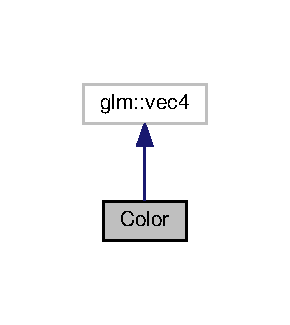
\includegraphics[width=139pt]{struct_color__inherit__graph}
\end{center}
\end{figure}


Collaboration diagram for Color\+:
\nopagebreak
\begin{figure}[H]
\begin{center}
\leavevmode
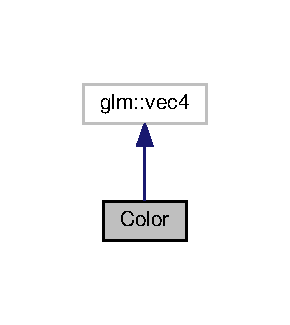
\includegraphics[width=139pt]{struct_color__coll__graph}
\end{center}
\end{figure}
\subsection*{Public Member Functions}
\begin{DoxyCompactItemize}
\item 
\hyperlink{struct_color_a9a742cbe9f9f4037f5d9f4e81a9b2428}{Color} ()
\item 
\hyperlink{struct_color_a373c542c99fb83ce9c7c08aae76b2718}{Color} (float r, float g, float b)
\item 
\hyperlink{struct_color_a6e4627389673c8b5cce81bf3eec79938}{Color} (float r, float g, float b, float a)
\item 
glm\+::vec4 \hyperlink{struct_color_aac52dbc4a7b5b5f500171fa74be323f6}{get\+G\+LM} ()
\end{DoxyCompactItemize}


\subsection{Detailed Description}


Definition at line 8 of file Color.\+h.



\subsection{Constructor \& Destructor Documentation}
\mbox{\Hypertarget{struct_color_a9a742cbe9f9f4037f5d9f4e81a9b2428}\label{struct_color_a9a742cbe9f9f4037f5d9f4e81a9b2428}} 
\index{Color@{Color}!Color@{Color}}
\index{Color@{Color}!Color@{Color}}
\subsubsection{\texorpdfstring{Color()}{Color()}\hspace{0.1cm}{\footnotesize\ttfamily [1/3]}}
{\footnotesize\ttfamily Color\+::\+Color (\begin{DoxyParamCaption}{ }\end{DoxyParamCaption})\hspace{0.3cm}{\ttfamily [inline]}}



Definition at line 10 of file Color.\+h.

\mbox{\Hypertarget{struct_color_a373c542c99fb83ce9c7c08aae76b2718}\label{struct_color_a373c542c99fb83ce9c7c08aae76b2718}} 
\index{Color@{Color}!Color@{Color}}
\index{Color@{Color}!Color@{Color}}
\subsubsection{\texorpdfstring{Color()}{Color()}\hspace{0.1cm}{\footnotesize\ttfamily [2/3]}}
{\footnotesize\ttfamily Color\+::\+Color (\begin{DoxyParamCaption}\item[{float}]{r,  }\item[{float}]{g,  }\item[{float}]{b }\end{DoxyParamCaption})\hspace{0.3cm}{\ttfamily [inline]}}



Definition at line 11 of file Color.\+h.

\mbox{\Hypertarget{struct_color_a6e4627389673c8b5cce81bf3eec79938}\label{struct_color_a6e4627389673c8b5cce81bf3eec79938}} 
\index{Color@{Color}!Color@{Color}}
\index{Color@{Color}!Color@{Color}}
\subsubsection{\texorpdfstring{Color()}{Color()}\hspace{0.1cm}{\footnotesize\ttfamily [3/3]}}
{\footnotesize\ttfamily Color\+::\+Color (\begin{DoxyParamCaption}\item[{float}]{r,  }\item[{float}]{g,  }\item[{float}]{b,  }\item[{float}]{a }\end{DoxyParamCaption})\hspace{0.3cm}{\ttfamily [inline]}}



Definition at line 12 of file Color.\+h.



\subsection{Member Function Documentation}
\mbox{\Hypertarget{struct_color_aac52dbc4a7b5b5f500171fa74be323f6}\label{struct_color_aac52dbc4a7b5b5f500171fa74be323f6}} 
\index{Color@{Color}!get\+G\+LM@{get\+G\+LM}}
\index{get\+G\+LM@{get\+G\+LM}!Color@{Color}}
\subsubsection{\texorpdfstring{get\+G\+L\+M()}{getGLM()}}
{\footnotesize\ttfamily glm\+::vec4 Color\+::get\+G\+LM (\begin{DoxyParamCaption}{ }\end{DoxyParamCaption})\hspace{0.3cm}{\ttfamily [inline]}}



Definition at line 14 of file Color.\+h.



The documentation for this struct was generated from the following file\+:\begin{DoxyCompactItemize}
\item 
/home/rory/\+Projects/ece-\/6122-\/final-\/project/src/objects/\hyperlink{_color_8h}{Color.\+h}\end{DoxyCompactItemize}

\hypertarget{struct_face}{}\section{Face Struct Reference}
\label{struct_face}\index{Face@{Face}}


{\ttfamily \#include $<$Face.\+h$>$}

\subsection*{Public Member Functions}
\begin{DoxyCompactItemize}
\item 
\hyperlink{struct_face_afdb634bc2d5287ba0d62e46b57e9dc2e}{Face} ()
\item 
\hyperlink{struct_face_acc432f36a78d2abdd6d7d7392299013c}{Face} (unsigned int px, unsigned int py, unsigned int pz, unsigned int tx, unsigned int ty, unsigned int tz, unsigned int nx, unsigned int ny, unsigned int nz)
\end{DoxyCompactItemize}
\subsection*{Public Attributes}
\begin{DoxyCompactItemize}
\item 
glm\+::uvec3 \hyperlink{struct_face_a5d796c13d0c71d4d5745ae0597380037}{position\+Indices}
\item 
glm\+::uvec3 \hyperlink{struct_face_abf7b5c4f1771b6ea979d1f38b107c0cf}{texcoord\+Indices}
\item 
glm\+::uvec3 \hyperlink{struct_face_a0d581c67d739a1372557e528b3dbb78a}{normal\+Indices}
\end{DoxyCompactItemize}


\subsection{Detailed Description}


Definition at line 7 of file Face.\+h.



\subsection{Constructor \& Destructor Documentation}
\mbox{\Hypertarget{struct_face_afdb634bc2d5287ba0d62e46b57e9dc2e}\label{struct_face_afdb634bc2d5287ba0d62e46b57e9dc2e}} 
\index{Face@{Face}!Face@{Face}}
\index{Face@{Face}!Face@{Face}}
\subsubsection{\texorpdfstring{Face()}{Face()}\hspace{0.1cm}{\footnotesize\ttfamily [1/2]}}
{\footnotesize\ttfamily Face\+::\+Face (\begin{DoxyParamCaption}{ }\end{DoxyParamCaption})\hspace{0.3cm}{\ttfamily [inline]}}



Definition at line 13 of file Face.\+h.

\mbox{\Hypertarget{struct_face_acc432f36a78d2abdd6d7d7392299013c}\label{struct_face_acc432f36a78d2abdd6d7d7392299013c}} 
\index{Face@{Face}!Face@{Face}}
\index{Face@{Face}!Face@{Face}}
\subsubsection{\texorpdfstring{Face()}{Face()}\hspace{0.1cm}{\footnotesize\ttfamily [2/2]}}
{\footnotesize\ttfamily Face\+::\+Face (\begin{DoxyParamCaption}\item[{unsigned int}]{px,  }\item[{unsigned int}]{py,  }\item[{unsigned int}]{pz,  }\item[{unsigned int}]{tx,  }\item[{unsigned int}]{ty,  }\item[{unsigned int}]{tz,  }\item[{unsigned int}]{nx,  }\item[{unsigned int}]{ny,  }\item[{unsigned int}]{nz }\end{DoxyParamCaption})\hspace{0.3cm}{\ttfamily [inline]}}



Definition at line 14 of file Face.\+h.



\subsection{Member Data Documentation}
\mbox{\Hypertarget{struct_face_a0d581c67d739a1372557e528b3dbb78a}\label{struct_face_a0d581c67d739a1372557e528b3dbb78a}} 
\index{Face@{Face}!normal\+Indices@{normal\+Indices}}
\index{normal\+Indices@{normal\+Indices}!Face@{Face}}
\subsubsection{\texorpdfstring{normal\+Indices}{normalIndices}}
{\footnotesize\ttfamily glm\+::uvec3 Face\+::normal\+Indices}



Definition at line 11 of file Face.\+h.

\mbox{\Hypertarget{struct_face_a5d796c13d0c71d4d5745ae0597380037}\label{struct_face_a5d796c13d0c71d4d5745ae0597380037}} 
\index{Face@{Face}!position\+Indices@{position\+Indices}}
\index{position\+Indices@{position\+Indices}!Face@{Face}}
\subsubsection{\texorpdfstring{position\+Indices}{positionIndices}}
{\footnotesize\ttfamily glm\+::uvec3 Face\+::position\+Indices}



Definition at line 9 of file Face.\+h.

\mbox{\Hypertarget{struct_face_abf7b5c4f1771b6ea979d1f38b107c0cf}\label{struct_face_abf7b5c4f1771b6ea979d1f38b107c0cf}} 
\index{Face@{Face}!texcoord\+Indices@{texcoord\+Indices}}
\index{texcoord\+Indices@{texcoord\+Indices}!Face@{Face}}
\subsubsection{\texorpdfstring{texcoord\+Indices}{texcoordIndices}}
{\footnotesize\ttfamily glm\+::uvec3 Face\+::texcoord\+Indices}



Definition at line 10 of file Face.\+h.



The documentation for this struct was generated from the following file\+:\begin{DoxyCompactItemize}
\item 
/home/rory/\+Projects/ece-\/6122-\/final-\/project/src/objects/\hyperlink{_face_8h}{Face.\+h}\end{DoxyCompactItemize}

\hypertarget{class_image_loader}{}\section{Image\+Loader Class Reference}
\label{class_image_loader}\index{Image\+Loader@{Image\+Loader}}


{\ttfamily \#include $<$Image\+Loader.\+h$>$}

\subsection*{Static Public Member Functions}
\begin{DoxyCompactItemize}
\item 
static unsigned char $\ast$ \hyperlink{class_image_loader_af2b82932ce07681d384ac827c48f76e7}{load} (const char $\ast$filepath, int $\ast$width, int $\ast$height)
\item 
static void \hyperlink{class_image_loader_a3b6851be17b336e8d5f7bf914d6aa971}{free} (unsigned char $\ast$bits)
\end{DoxyCompactItemize}


\subsection{Detailed Description}


Definition at line 5 of file Image\+Loader.\+h.



\subsection{Member Function Documentation}
\mbox{\Hypertarget{class_image_loader_a3b6851be17b336e8d5f7bf914d6aa971}\label{class_image_loader_a3b6851be17b336e8d5f7bf914d6aa971}} 
\index{Image\+Loader@{Image\+Loader}!free@{free}}
\index{free@{free}!Image\+Loader@{Image\+Loader}}
\subsubsection{\texorpdfstring{free()}{free()}}
{\footnotesize\ttfamily void Image\+Loader\+::free (\begin{DoxyParamCaption}\item[{unsigned char $\ast$}]{bits }\end{DoxyParamCaption})\hspace{0.3cm}{\ttfamily [static]}}



Definition at line 36 of file Image\+Loader.\+cpp.

\mbox{\Hypertarget{class_image_loader_af2b82932ce07681d384ac827c48f76e7}\label{class_image_loader_af2b82932ce07681d384ac827c48f76e7}} 
\index{Image\+Loader@{Image\+Loader}!load@{load}}
\index{load@{load}!Image\+Loader@{Image\+Loader}}
\subsubsection{\texorpdfstring{load()}{load()}}
{\footnotesize\ttfamily unsigned char $\ast$ Image\+Loader\+::load (\begin{DoxyParamCaption}\item[{const char $\ast$}]{filepath,  }\item[{int $\ast$}]{width,  }\item[{int $\ast$}]{height }\end{DoxyParamCaption})\hspace{0.3cm}{\ttfamily [static]}}



Definition at line 4 of file Image\+Loader.\+cpp.



The documentation for this class was generated from the following files\+:\begin{DoxyCompactItemize}
\item 
/home/rory/\+Projects/ece-\/6122-\/final-\/project/src/utils/\hyperlink{_image_loader_8h}{Image\+Loader.\+h}\item 
/home/rory/\+Projects/ece-\/6122-\/final-\/project/src/utils/\hyperlink{_image_loader_8cpp}{Image\+Loader.\+cpp}\end{DoxyCompactItemize}

\hypertarget{class_layer}{}\section{Layer Class Reference}
\label{class_layer}\index{Layer@{Layer}}


{\ttfamily \#include $<$Layer.\+h$>$}



Collaboration diagram for Layer\+:
\nopagebreak
\begin{figure}[H]
\begin{center}
\leavevmode
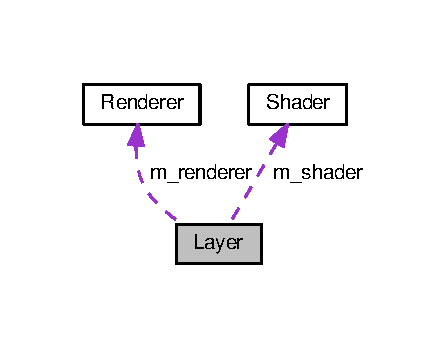
\includegraphics[width=214pt]{class_layer__coll__graph}
\end{center}
\end{figure}
\subsection*{Public Member Functions}
\begin{DoxyCompactItemize}
\item 
\hyperlink{class_layer_ad5cb744328eb91a6c0670efe57a9afbd}{Layer} (\hyperlink{class_shader}{Shader} $\ast$shader)
\item 
\hyperlink{class_layer_a1b1ba4804451dfe6cc357194e42762ae}{$\sim$\+Layer} ()
\item 
void \hyperlink{class_layer_aa1e828db7d673a1083aa2eb211663628}{add} (\hyperlink{class_object}{Object} $\ast$object)
\item 
void \hyperlink{class_layer_ad8f9382947a2b1093bf1c8846751bfa2}{render} (const glm\+::vec3 \&eye\+Position)
\item 
const std\+::vector$<$ \hyperlink{class_object}{Object} $\ast$ $>$ \& \hyperlink{class_layer_ac22c1bfa8ac715224adcf27409019e9f}{get\+Objects} ()
\item 
\hyperlink{class_object}{Object} $\ast$ \hyperlink{class_layer_ae51468bd68ee2ba01571efc430ac666f}{get\+Object} (int index)
\end{DoxyCompactItemize}
\subsection*{Protected Member Functions}
\begin{DoxyCompactItemize}
\item 
\hyperlink{class_layer_a4fe3c6314cb78fef7ffef3f6439fc195}{Layer} (\hyperlink{class_renderer}{Renderer} $\ast$renderer, \hyperlink{class_shader}{Shader} $\ast$shader)
\end{DoxyCompactItemize}
\subsection*{Protected Attributes}
\begin{DoxyCompactItemize}
\item 
\hyperlink{class_renderer}{Renderer} $\ast$ \hyperlink{class_layer_a37e53fc9b8764c7fa4b69de8f037a76f}{m\+\_\+renderer}
\item 
std\+::vector$<$ \hyperlink{class_object}{Object} $\ast$ $>$ \hyperlink{class_layer_a5dd19348285314342a7721c000c97179}{m\+\_\+objects}
\item 
\hyperlink{class_shader}{Shader} $\ast$ \hyperlink{class_layer_aa7cd5a12a7862c9127316d065278f5cc}{m\+\_\+shader}
\end{DoxyCompactItemize}


\subsection{Detailed Description}


Definition at line 10 of file Layer.\+h.



\subsection{Constructor \& Destructor Documentation}
\mbox{\Hypertarget{class_layer_ad5cb744328eb91a6c0670efe57a9afbd}\label{class_layer_ad5cb744328eb91a6c0670efe57a9afbd}} 
\index{Layer@{Layer}!Layer@{Layer}}
\index{Layer@{Layer}!Layer@{Layer}}
\subsubsection{\texorpdfstring{Layer()}{Layer()}\hspace{0.1cm}{\footnotesize\ttfamily [1/2]}}
{\footnotesize\ttfamily Layer\+::\+Layer (\begin{DoxyParamCaption}\item[{\hyperlink{class_shader}{Shader} $\ast$}]{shader }\end{DoxyParamCaption})}

Constructor 
\begin{DoxyParams}{Parameters}
{\em shader} & T\+O\+DO \\
\hline
\end{DoxyParams}


Definition at line 7 of file Layer.\+cpp.

\mbox{\Hypertarget{class_layer_a1b1ba4804451dfe6cc357194e42762ae}\label{class_layer_a1b1ba4804451dfe6cc357194e42762ae}} 
\index{Layer@{Layer}!````~Layer@{$\sim$\+Layer}}
\index{````~Layer@{$\sim$\+Layer}!Layer@{Layer}}
\subsubsection{\texorpdfstring{$\sim$\+Layer()}{~Layer()}}
{\footnotesize\ttfamily Layer\+::$\sim$\+Layer (\begin{DoxyParamCaption}{ }\end{DoxyParamCaption})}

Destructor 

Definition at line 26 of file Layer.\+cpp.

\mbox{\Hypertarget{class_layer_a4fe3c6314cb78fef7ffef3f6439fc195}\label{class_layer_a4fe3c6314cb78fef7ffef3f6439fc195}} 
\index{Layer@{Layer}!Layer@{Layer}}
\index{Layer@{Layer}!Layer@{Layer}}
\subsubsection{\texorpdfstring{Layer()}{Layer()}\hspace{0.1cm}{\footnotesize\ttfamily [2/2]}}
{\footnotesize\ttfamily Layer\+::\+Layer (\begin{DoxyParamCaption}\item[{\hyperlink{class_renderer}{Renderer} $\ast$}]{renderer,  }\item[{\hyperlink{class_shader}{Shader} $\ast$}]{shader }\end{DoxyParamCaption})\hspace{0.3cm}{\ttfamily [protected]}}

Constructor 
\begin{DoxyParams}{Parameters}
{\em renderer} & T\+O\+DO \\
\hline
{\em shader} & T\+O\+DO \\
\hline
{\em pmat} & T\+O\+DO \\
\hline
\end{DoxyParams}


Definition at line 18 of file Layer.\+cpp.



\subsection{Member Function Documentation}
\mbox{\Hypertarget{class_layer_aa1e828db7d673a1083aa2eb211663628}\label{class_layer_aa1e828db7d673a1083aa2eb211663628}} 
\index{Layer@{Layer}!add@{add}}
\index{add@{add}!Layer@{Layer}}
\subsubsection{\texorpdfstring{add()}{add()}}
{\footnotesize\ttfamily void Layer\+::add (\begin{DoxyParamCaption}\item[{\hyperlink{class_object}{Object} $\ast$}]{object }\end{DoxyParamCaption})}

Adds (pushes back) a shape to the layer 
\begin{DoxyParams}{Parameters}
{\em shape} & The object to add \\
\hline
\end{DoxyParams}


Definition at line 35 of file Layer.\+cpp.

\mbox{\Hypertarget{class_layer_ae51468bd68ee2ba01571efc430ac666f}\label{class_layer_ae51468bd68ee2ba01571efc430ac666f}} 
\index{Layer@{Layer}!get\+Object@{get\+Object}}
\index{get\+Object@{get\+Object}!Layer@{Layer}}
\subsubsection{\texorpdfstring{get\+Object()}{getObject()}}
{\footnotesize\ttfamily \hyperlink{class_object}{Object} $\ast$ Layer\+::get\+Object (\begin{DoxyParamCaption}\item[{int}]{index }\end{DoxyParamCaption})}

Returns the object by index 
\begin{DoxyParams}{Parameters}
{\em index} & The index into the object array \\
\hline
\end{DoxyParams}
\begin{DoxyReturn}{Returns}
Returns the pointer to the object on success, else N\+U\+LL 
\end{DoxyReturn}


Definition at line 62 of file Layer.\+cpp.

\mbox{\Hypertarget{class_layer_ac22c1bfa8ac715224adcf27409019e9f}\label{class_layer_ac22c1bfa8ac715224adcf27409019e9f}} 
\index{Layer@{Layer}!get\+Objects@{get\+Objects}}
\index{get\+Objects@{get\+Objects}!Layer@{Layer}}
\subsubsection{\texorpdfstring{get\+Objects()}{getObjects()}}
{\footnotesize\ttfamily const std\+::vector$<$ \hyperlink{class_object}{Object} $\ast$ $>$ \& Layer\+::get\+Objects (\begin{DoxyParamCaption}{ }\end{DoxyParamCaption})}

Get all the objects in this layer \begin{DoxyReturn}{Returns}
Returns all the objects in this layer 
\end{DoxyReturn}


Definition at line 73 of file Layer.\+cpp.

\mbox{\Hypertarget{class_layer_ad8f9382947a2b1093bf1c8846751bfa2}\label{class_layer_ad8f9382947a2b1093bf1c8846751bfa2}} 
\index{Layer@{Layer}!render@{render}}
\index{render@{render}!Layer@{Layer}}
\subsubsection{\texorpdfstring{render()}{render()}}
{\footnotesize\ttfamily void Layer\+::render (\begin{DoxyParamCaption}\item[{const glm\+::vec3 \&}]{eye\+Position }\end{DoxyParamCaption})}

Renders the layer by submitting the objects to the \hyperlink{class_renderer}{Renderer}, then flushing the \hyperlink{class_renderer}{Renderer} buffer (aka draw the triangles) 

Definition at line 44 of file Layer.\+cpp.



\subsection{Member Data Documentation}
\mbox{\Hypertarget{class_layer_a5dd19348285314342a7721c000c97179}\label{class_layer_a5dd19348285314342a7721c000c97179}} 
\index{Layer@{Layer}!m\+\_\+objects@{m\+\_\+objects}}
\index{m\+\_\+objects@{m\+\_\+objects}!Layer@{Layer}}
\subsubsection{\texorpdfstring{m\+\_\+objects}{m\_objects}}
{\footnotesize\ttfamily std\+::vector$<$\hyperlink{class_object}{Object} $\ast$$>$ Layer\+::m\+\_\+objects\hspace{0.3cm}{\ttfamily [protected]}}



Definition at line 26 of file Layer.\+h.

\mbox{\Hypertarget{class_layer_a37e53fc9b8764c7fa4b69de8f037a76f}\label{class_layer_a37e53fc9b8764c7fa4b69de8f037a76f}} 
\index{Layer@{Layer}!m\+\_\+renderer@{m\+\_\+renderer}}
\index{m\+\_\+renderer@{m\+\_\+renderer}!Layer@{Layer}}
\subsubsection{\texorpdfstring{m\+\_\+renderer}{m\_renderer}}
{\footnotesize\ttfamily \hyperlink{class_renderer}{Renderer}$\ast$ Layer\+::m\+\_\+renderer\hspace{0.3cm}{\ttfamily [protected]}}



Definition at line 25 of file Layer.\+h.

\mbox{\Hypertarget{class_layer_aa7cd5a12a7862c9127316d065278f5cc}\label{class_layer_aa7cd5a12a7862c9127316d065278f5cc}} 
\index{Layer@{Layer}!m\+\_\+shader@{m\+\_\+shader}}
\index{m\+\_\+shader@{m\+\_\+shader}!Layer@{Layer}}
\subsubsection{\texorpdfstring{m\+\_\+shader}{m\_shader}}
{\footnotesize\ttfamily \hyperlink{class_shader}{Shader}$\ast$ Layer\+::m\+\_\+shader\hspace{0.3cm}{\ttfamily [protected]}}



Definition at line 27 of file Layer.\+h.



The documentation for this class was generated from the following files\+:\begin{DoxyCompactItemize}
\item 
/home/rory/\+Projects/ece-\/6122-\/final-\/project/src/\hyperlink{_layer_8h}{Layer.\+h}\item 
/home/rory/\+Projects/ece-\/6122-\/final-\/project/src/\hyperlink{_layer_8cpp}{Layer.\+cpp}\end{DoxyCompactItemize}

\hypertarget{class_material}{}\section{Material Class Reference}
\label{class_material}\index{Material@{Material}}


{\ttfamily \#include $<$Material.\+h$>$}

\subsection*{Public Member Functions}
\begin{DoxyCompactItemize}
\item 
\hyperlink{class_material_a137e987401b63eb7c6c27c3e38bc74b5}{Material} ()
\item 
void \hyperlink{class_material_a8d3228e94c92ffffc1c5a9504ee5fd90}{set\+Name} (std\+::string name)
\item 
void \hyperlink{class_material_ad166d6c2ae9bc2ae460f5912ef913914}{set\+Ambient} (glm\+::vec3 Ka)
\item 
void \hyperlink{class_material_a4cb374db09a8167ebf36ab17fd373fe3}{set\+Diffuse} (glm\+::vec3 Kd)
\item 
void \hyperlink{class_material_af55a5fefcf54ddac103e254298381c42}{set\+Specular} (glm\+::vec3 Ks)
\item 
void \hyperlink{class_material_a82a92812bac1ee728bd11816cb3217f5}{set\+Emission} (glm\+::vec3 Ke)
\item 
void \hyperlink{class_material_a329d0ae8403956a71b1d45b3284f7dd7}{set\+Shininess} (float shininess)
\item 
void \hyperlink{class_material_aa7eeda191689ff20ec61750440c39427}{set\+Refraction} (float Ni)
\item 
void \hyperlink{class_material_a76c5ad9250191eed374fb6d896efd0bb}{set\+Specular\+Exponent} (float Ns)
\item 
void \hyperlink{class_material_a5974bc8810af827031f0697d21418c3a}{set\+Dissolve\+Factor} (float d)
\item 
void \hyperlink{class_material_ae5fc41aae479cbae2b85c9f581759767}{set\+Illumination} (unsigned int illum)
\item 
void \hyperlink{class_material_a6b219cb34ef48da8feb6c03459a5c30d}{set\+Shading\+Model} (int model)
\item 
void \hyperlink{class_material_a3e20f3c7602300c54b2e8b5ee1c73c42}{set\+Blend\+Func} (int blend\+Func)
\item 
void \hyperlink{class_material_ab7326632dff9200c9e4e2c9aa98fed60}{set\+Wireframe} (int enable)
\item 
const std\+::string \& \hyperlink{class_material_ab51bcfb064df3fa0ec1a5062e873fe49}{get\+Name} () const
\item 
const glm\+::vec3 \& \hyperlink{class_material_a61bafc60f2755cc546f3a6dc5736a6ae}{get\+Ambient} () const
\item 
const glm\+::vec3 \& \hyperlink{class_material_a6d7a33e9240d886dd6e62782e380f05e}{get\+Diffuse} () const
\item 
const glm\+::vec3 \& \hyperlink{class_material_a1781994da525d08bfb6d48187274d0a6}{get\+Specular} () const
\item 
const glm\+::vec3 \& \hyperlink{class_material_a3c58519af3fdbf5bc3f5a6e1712d8fc6}{get\+Emission} () const
\item 
const float \& \hyperlink{class_material_ae33424535bcfceb95632e09492d33972}{get\+Shininess} () const
\item 
const float \& \hyperlink{class_material_a3c90133f63f8ac1ba05359461234b6a7}{get\+Refraction} () const
\item 
const float \& \hyperlink{class_material_a4087dd55f6d034d3011dafeeeed1ad2d}{get\+Specular\+Exponent} () const
\item 
const float \& \hyperlink{class_material_ae615c797e56c8ad228888e8f21fd8223}{get\+Dissolve\+Factor} () const
\item 
const unsigned int \& \hyperlink{class_material_a30f8ed7054d7f09c42642b28e96a6635}{get\+Illumination} () const
\item 
const int \& \hyperlink{class_material_a50ad1d1911490e2458f841b4e8195823}{get\+Shading\+Model} () const
\item 
const int \& \hyperlink{class_material_ac8bb3627639e5454d58e9a9553ed1654}{get\+Blend\+Func} () const
\item 
const int \& \hyperlink{class_material_ad1be512566174cd3b091a6e3479a2440}{get\+Wireframe} () const
\end{DoxyCompactItemize}


\subsection{Detailed Description}
What do each of the material properties mean? Ka\+: Ambient T\+O\+DO briefly explain Kd\+: Diffuse T\+O\+DO briefly explain Ks\+: Specular T\+O\+DO briefly explain Ke\+: T\+O\+DO briefly explain shininess\+: T\+O\+DO briefly explain Ni\+: T\+O\+DO briefly explain Ns\+: T\+O\+DO briefly explain d\+: T\+O\+DO briefly explain illum\+: 0. \hyperlink{struct_color}{Color} on and Ambient off
\begin{DoxyEnumerate}
\item \hyperlink{struct_color}{Color} on and Ambient on
\item Highlight on
\item Reflection on and Ray trace on
\item Transparency\+: Glass on, Reflection\+: Ray trace on
\item Reflection\+: Fresnel on and Ray trace on
\item Transparency\+: Refraction on, Reflection\+: Fresnel off and Ray trace on
\item Transparency\+: Refraction on, Reflection\+: Fresnel on and Ray trace on
\item Reflection on and Ray trace off
\item Transparency\+: Glass on, Reflection\+: Ray trace off
\item Casts shadows onto invisible surfaces
\end{DoxyEnumerate}

The color includes an ambient constant term, and a diffuse and specular shading term for each light source. The formula is\+: color = Ka\+Ia + Kd \{ S\+UM j=1..ls, (N$\ast$\+Lj)Ij \} + Ks \{ S\+UM j=1..ls, ((H$\ast$\+Hj)$^\wedge$\+Ns)Ij \}

Term definitions are\+: Ia ambient light, Ij light j\textquotesingle{}s intensity, Ka ambient reflectance, Kd diffuse reflectance, Ks specular reflectance, H unit vector bisector between L and V, L unit light vector, N unit surface normal, V unit view vector 

Definition at line 45 of file Material.\+h.



\subsection{Constructor \& Destructor Documentation}
\mbox{\Hypertarget{class_material_a137e987401b63eb7c6c27c3e38bc74b5}\label{class_material_a137e987401b63eb7c6c27c3e38bc74b5}} 
\index{Material@{Material}!Material@{Material}}
\index{Material@{Material}!Material@{Material}}
\subsubsection{\texorpdfstring{Material()}{Material()}}
{\footnotesize\ttfamily Material\+::\+Material (\begin{DoxyParamCaption}{ }\end{DoxyParamCaption})}

Constructor 

Definition at line 6 of file Material.\+cpp.



\subsection{Member Function Documentation}
\mbox{\Hypertarget{class_material_a61bafc60f2755cc546f3a6dc5736a6ae}\label{class_material_a61bafc60f2755cc546f3a6dc5736a6ae}} 
\index{Material@{Material}!get\+Ambient@{get\+Ambient}}
\index{get\+Ambient@{get\+Ambient}!Material@{Material}}
\subsubsection{\texorpdfstring{get\+Ambient()}{getAmbient()}}
{\footnotesize\ttfamily const glm\+::vec3\& Material\+::get\+Ambient (\begin{DoxyParamCaption}{ }\end{DoxyParamCaption}) const\hspace{0.3cm}{\ttfamily [inline]}}



Definition at line 65 of file Material.\+h.

\mbox{\Hypertarget{class_material_ac8bb3627639e5454d58e9a9553ed1654}\label{class_material_ac8bb3627639e5454d58e9a9553ed1654}} 
\index{Material@{Material}!get\+Blend\+Func@{get\+Blend\+Func}}
\index{get\+Blend\+Func@{get\+Blend\+Func}!Material@{Material}}
\subsubsection{\texorpdfstring{get\+Blend\+Func()}{getBlendFunc()}}
{\footnotesize\ttfamily const int\& Material\+::get\+Blend\+Func (\begin{DoxyParamCaption}{ }\end{DoxyParamCaption}) const\hspace{0.3cm}{\ttfamily [inline]}}



Definition at line 75 of file Material.\+h.

\mbox{\Hypertarget{class_material_a6d7a33e9240d886dd6e62782e380f05e}\label{class_material_a6d7a33e9240d886dd6e62782e380f05e}} 
\index{Material@{Material}!get\+Diffuse@{get\+Diffuse}}
\index{get\+Diffuse@{get\+Diffuse}!Material@{Material}}
\subsubsection{\texorpdfstring{get\+Diffuse()}{getDiffuse()}}
{\footnotesize\ttfamily const glm\+::vec3\& Material\+::get\+Diffuse (\begin{DoxyParamCaption}{ }\end{DoxyParamCaption}) const\hspace{0.3cm}{\ttfamily [inline]}}



Definition at line 66 of file Material.\+h.

\mbox{\Hypertarget{class_material_ae615c797e56c8ad228888e8f21fd8223}\label{class_material_ae615c797e56c8ad228888e8f21fd8223}} 
\index{Material@{Material}!get\+Dissolve\+Factor@{get\+Dissolve\+Factor}}
\index{get\+Dissolve\+Factor@{get\+Dissolve\+Factor}!Material@{Material}}
\subsubsection{\texorpdfstring{get\+Dissolve\+Factor()}{getDissolveFactor()}}
{\footnotesize\ttfamily const float\& Material\+::get\+Dissolve\+Factor (\begin{DoxyParamCaption}{ }\end{DoxyParamCaption}) const\hspace{0.3cm}{\ttfamily [inline]}}



Definition at line 72 of file Material.\+h.

\mbox{\Hypertarget{class_material_a3c58519af3fdbf5bc3f5a6e1712d8fc6}\label{class_material_a3c58519af3fdbf5bc3f5a6e1712d8fc6}} 
\index{Material@{Material}!get\+Emission@{get\+Emission}}
\index{get\+Emission@{get\+Emission}!Material@{Material}}
\subsubsection{\texorpdfstring{get\+Emission()}{getEmission()}}
{\footnotesize\ttfamily const glm\+::vec3\& Material\+::get\+Emission (\begin{DoxyParamCaption}{ }\end{DoxyParamCaption}) const\hspace{0.3cm}{\ttfamily [inline]}}



Definition at line 68 of file Material.\+h.

\mbox{\Hypertarget{class_material_a30f8ed7054d7f09c42642b28e96a6635}\label{class_material_a30f8ed7054d7f09c42642b28e96a6635}} 
\index{Material@{Material}!get\+Illumination@{get\+Illumination}}
\index{get\+Illumination@{get\+Illumination}!Material@{Material}}
\subsubsection{\texorpdfstring{get\+Illumination()}{getIllumination()}}
{\footnotesize\ttfamily const unsigned int\& Material\+::get\+Illumination (\begin{DoxyParamCaption}{ }\end{DoxyParamCaption}) const\hspace{0.3cm}{\ttfamily [inline]}}



Definition at line 73 of file Material.\+h.

\mbox{\Hypertarget{class_material_ab51bcfb064df3fa0ec1a5062e873fe49}\label{class_material_ab51bcfb064df3fa0ec1a5062e873fe49}} 
\index{Material@{Material}!get\+Name@{get\+Name}}
\index{get\+Name@{get\+Name}!Material@{Material}}
\subsubsection{\texorpdfstring{get\+Name()}{getName()}}
{\footnotesize\ttfamily const std\+::string\& Material\+::get\+Name (\begin{DoxyParamCaption}{ }\end{DoxyParamCaption}) const\hspace{0.3cm}{\ttfamily [inline]}}



Definition at line 64 of file Material.\+h.

\mbox{\Hypertarget{class_material_a3c90133f63f8ac1ba05359461234b6a7}\label{class_material_a3c90133f63f8ac1ba05359461234b6a7}} 
\index{Material@{Material}!get\+Refraction@{get\+Refraction}}
\index{get\+Refraction@{get\+Refraction}!Material@{Material}}
\subsubsection{\texorpdfstring{get\+Refraction()}{getRefraction()}}
{\footnotesize\ttfamily const float\& Material\+::get\+Refraction (\begin{DoxyParamCaption}{ }\end{DoxyParamCaption}) const\hspace{0.3cm}{\ttfamily [inline]}}



Definition at line 70 of file Material.\+h.

\mbox{\Hypertarget{class_material_a50ad1d1911490e2458f841b4e8195823}\label{class_material_a50ad1d1911490e2458f841b4e8195823}} 
\index{Material@{Material}!get\+Shading\+Model@{get\+Shading\+Model}}
\index{get\+Shading\+Model@{get\+Shading\+Model}!Material@{Material}}
\subsubsection{\texorpdfstring{get\+Shading\+Model()}{getShadingModel()}}
{\footnotesize\ttfamily const int\& Material\+::get\+Shading\+Model (\begin{DoxyParamCaption}{ }\end{DoxyParamCaption}) const\hspace{0.3cm}{\ttfamily [inline]}}



Definition at line 74 of file Material.\+h.

\mbox{\Hypertarget{class_material_ae33424535bcfceb95632e09492d33972}\label{class_material_ae33424535bcfceb95632e09492d33972}} 
\index{Material@{Material}!get\+Shininess@{get\+Shininess}}
\index{get\+Shininess@{get\+Shininess}!Material@{Material}}
\subsubsection{\texorpdfstring{get\+Shininess()}{getShininess()}}
{\footnotesize\ttfamily const float\& Material\+::get\+Shininess (\begin{DoxyParamCaption}{ }\end{DoxyParamCaption}) const\hspace{0.3cm}{\ttfamily [inline]}}



Definition at line 69 of file Material.\+h.

\mbox{\Hypertarget{class_material_a1781994da525d08bfb6d48187274d0a6}\label{class_material_a1781994da525d08bfb6d48187274d0a6}} 
\index{Material@{Material}!get\+Specular@{get\+Specular}}
\index{get\+Specular@{get\+Specular}!Material@{Material}}
\subsubsection{\texorpdfstring{get\+Specular()}{getSpecular()}}
{\footnotesize\ttfamily const glm\+::vec3\& Material\+::get\+Specular (\begin{DoxyParamCaption}{ }\end{DoxyParamCaption}) const\hspace{0.3cm}{\ttfamily [inline]}}



Definition at line 67 of file Material.\+h.

\mbox{\Hypertarget{class_material_a4087dd55f6d034d3011dafeeeed1ad2d}\label{class_material_a4087dd55f6d034d3011dafeeeed1ad2d}} 
\index{Material@{Material}!get\+Specular\+Exponent@{get\+Specular\+Exponent}}
\index{get\+Specular\+Exponent@{get\+Specular\+Exponent}!Material@{Material}}
\subsubsection{\texorpdfstring{get\+Specular\+Exponent()}{getSpecularExponent()}}
{\footnotesize\ttfamily const float\& Material\+::get\+Specular\+Exponent (\begin{DoxyParamCaption}{ }\end{DoxyParamCaption}) const\hspace{0.3cm}{\ttfamily [inline]}}



Definition at line 71 of file Material.\+h.

\mbox{\Hypertarget{class_material_ad1be512566174cd3b091a6e3479a2440}\label{class_material_ad1be512566174cd3b091a6e3479a2440}} 
\index{Material@{Material}!get\+Wireframe@{get\+Wireframe}}
\index{get\+Wireframe@{get\+Wireframe}!Material@{Material}}
\subsubsection{\texorpdfstring{get\+Wireframe()}{getWireframe()}}
{\footnotesize\ttfamily const int\& Material\+::get\+Wireframe (\begin{DoxyParamCaption}{ }\end{DoxyParamCaption}) const\hspace{0.3cm}{\ttfamily [inline]}}



Definition at line 76 of file Material.\+h.

\mbox{\Hypertarget{class_material_ad166d6c2ae9bc2ae460f5912ef913914}\label{class_material_ad166d6c2ae9bc2ae460f5912ef913914}} 
\index{Material@{Material}!set\+Ambient@{set\+Ambient}}
\index{set\+Ambient@{set\+Ambient}!Material@{Material}}
\subsubsection{\texorpdfstring{set\+Ambient()}{setAmbient()}}
{\footnotesize\ttfamily void Material\+::set\+Ambient (\begin{DoxyParamCaption}\item[{glm\+::vec3}]{Ka }\end{DoxyParamCaption})\hspace{0.3cm}{\ttfamily [inline]}}



Definition at line 51 of file Material.\+h.

\mbox{\Hypertarget{class_material_a3e20f3c7602300c54b2e8b5ee1c73c42}\label{class_material_a3e20f3c7602300c54b2e8b5ee1c73c42}} 
\index{Material@{Material}!set\+Blend\+Func@{set\+Blend\+Func}}
\index{set\+Blend\+Func@{set\+Blend\+Func}!Material@{Material}}
\subsubsection{\texorpdfstring{set\+Blend\+Func()}{setBlendFunc()}}
{\footnotesize\ttfamily void Material\+::set\+Blend\+Func (\begin{DoxyParamCaption}\item[{int}]{blend\+Func }\end{DoxyParamCaption})\hspace{0.3cm}{\ttfamily [inline]}}



Definition at line 61 of file Material.\+h.

\mbox{\Hypertarget{class_material_a4cb374db09a8167ebf36ab17fd373fe3}\label{class_material_a4cb374db09a8167ebf36ab17fd373fe3}} 
\index{Material@{Material}!set\+Diffuse@{set\+Diffuse}}
\index{set\+Diffuse@{set\+Diffuse}!Material@{Material}}
\subsubsection{\texorpdfstring{set\+Diffuse()}{setDiffuse()}}
{\footnotesize\ttfamily void Material\+::set\+Diffuse (\begin{DoxyParamCaption}\item[{glm\+::vec3}]{Kd }\end{DoxyParamCaption})\hspace{0.3cm}{\ttfamily [inline]}}



Definition at line 52 of file Material.\+h.

\mbox{\Hypertarget{class_material_a5974bc8810af827031f0697d21418c3a}\label{class_material_a5974bc8810af827031f0697d21418c3a}} 
\index{Material@{Material}!set\+Dissolve\+Factor@{set\+Dissolve\+Factor}}
\index{set\+Dissolve\+Factor@{set\+Dissolve\+Factor}!Material@{Material}}
\subsubsection{\texorpdfstring{set\+Dissolve\+Factor()}{setDissolveFactor()}}
{\footnotesize\ttfamily void Material\+::set\+Dissolve\+Factor (\begin{DoxyParamCaption}\item[{float}]{d }\end{DoxyParamCaption})\hspace{0.3cm}{\ttfamily [inline]}}



Definition at line 58 of file Material.\+h.

\mbox{\Hypertarget{class_material_a82a92812bac1ee728bd11816cb3217f5}\label{class_material_a82a92812bac1ee728bd11816cb3217f5}} 
\index{Material@{Material}!set\+Emission@{set\+Emission}}
\index{set\+Emission@{set\+Emission}!Material@{Material}}
\subsubsection{\texorpdfstring{set\+Emission()}{setEmission()}}
{\footnotesize\ttfamily void Material\+::set\+Emission (\begin{DoxyParamCaption}\item[{glm\+::vec3}]{Ke }\end{DoxyParamCaption})\hspace{0.3cm}{\ttfamily [inline]}}



Definition at line 54 of file Material.\+h.

\mbox{\Hypertarget{class_material_ae5fc41aae479cbae2b85c9f581759767}\label{class_material_ae5fc41aae479cbae2b85c9f581759767}} 
\index{Material@{Material}!set\+Illumination@{set\+Illumination}}
\index{set\+Illumination@{set\+Illumination}!Material@{Material}}
\subsubsection{\texorpdfstring{set\+Illumination()}{setIllumination()}}
{\footnotesize\ttfamily void Material\+::set\+Illumination (\begin{DoxyParamCaption}\item[{unsigned int}]{illum }\end{DoxyParamCaption})\hspace{0.3cm}{\ttfamily [inline]}}



Definition at line 59 of file Material.\+h.

\mbox{\Hypertarget{class_material_a8d3228e94c92ffffc1c5a9504ee5fd90}\label{class_material_a8d3228e94c92ffffc1c5a9504ee5fd90}} 
\index{Material@{Material}!set\+Name@{set\+Name}}
\index{set\+Name@{set\+Name}!Material@{Material}}
\subsubsection{\texorpdfstring{set\+Name()}{setName()}}
{\footnotesize\ttfamily void Material\+::set\+Name (\begin{DoxyParamCaption}\item[{std\+::string}]{name }\end{DoxyParamCaption})\hspace{0.3cm}{\ttfamily [inline]}}



Definition at line 50 of file Material.\+h.

\mbox{\Hypertarget{class_material_aa7eeda191689ff20ec61750440c39427}\label{class_material_aa7eeda191689ff20ec61750440c39427}} 
\index{Material@{Material}!set\+Refraction@{set\+Refraction}}
\index{set\+Refraction@{set\+Refraction}!Material@{Material}}
\subsubsection{\texorpdfstring{set\+Refraction()}{setRefraction()}}
{\footnotesize\ttfamily void Material\+::set\+Refraction (\begin{DoxyParamCaption}\item[{float}]{Ni }\end{DoxyParamCaption})\hspace{0.3cm}{\ttfamily [inline]}}



Definition at line 56 of file Material.\+h.

\mbox{\Hypertarget{class_material_a6b219cb34ef48da8feb6c03459a5c30d}\label{class_material_a6b219cb34ef48da8feb6c03459a5c30d}} 
\index{Material@{Material}!set\+Shading\+Model@{set\+Shading\+Model}}
\index{set\+Shading\+Model@{set\+Shading\+Model}!Material@{Material}}
\subsubsection{\texorpdfstring{set\+Shading\+Model()}{setShadingModel()}}
{\footnotesize\ttfamily void Material\+::set\+Shading\+Model (\begin{DoxyParamCaption}\item[{int}]{model }\end{DoxyParamCaption})\hspace{0.3cm}{\ttfamily [inline]}}



Definition at line 60 of file Material.\+h.

\mbox{\Hypertarget{class_material_a329d0ae8403956a71b1d45b3284f7dd7}\label{class_material_a329d0ae8403956a71b1d45b3284f7dd7}} 
\index{Material@{Material}!set\+Shininess@{set\+Shininess}}
\index{set\+Shininess@{set\+Shininess}!Material@{Material}}
\subsubsection{\texorpdfstring{set\+Shininess()}{setShininess()}}
{\footnotesize\ttfamily void Material\+::set\+Shininess (\begin{DoxyParamCaption}\item[{float}]{shininess }\end{DoxyParamCaption})\hspace{0.3cm}{\ttfamily [inline]}}



Definition at line 55 of file Material.\+h.

\mbox{\Hypertarget{class_material_af55a5fefcf54ddac103e254298381c42}\label{class_material_af55a5fefcf54ddac103e254298381c42}} 
\index{Material@{Material}!set\+Specular@{set\+Specular}}
\index{set\+Specular@{set\+Specular}!Material@{Material}}
\subsubsection{\texorpdfstring{set\+Specular()}{setSpecular()}}
{\footnotesize\ttfamily void Material\+::set\+Specular (\begin{DoxyParamCaption}\item[{glm\+::vec3}]{Ks }\end{DoxyParamCaption})\hspace{0.3cm}{\ttfamily [inline]}}



Definition at line 53 of file Material.\+h.

\mbox{\Hypertarget{class_material_a76c5ad9250191eed374fb6d896efd0bb}\label{class_material_a76c5ad9250191eed374fb6d896efd0bb}} 
\index{Material@{Material}!set\+Specular\+Exponent@{set\+Specular\+Exponent}}
\index{set\+Specular\+Exponent@{set\+Specular\+Exponent}!Material@{Material}}
\subsubsection{\texorpdfstring{set\+Specular\+Exponent()}{setSpecularExponent()}}
{\footnotesize\ttfamily void Material\+::set\+Specular\+Exponent (\begin{DoxyParamCaption}\item[{float}]{Ns }\end{DoxyParamCaption})\hspace{0.3cm}{\ttfamily [inline]}}



Definition at line 57 of file Material.\+h.

\mbox{\Hypertarget{class_material_ab7326632dff9200c9e4e2c9aa98fed60}\label{class_material_ab7326632dff9200c9e4e2c9aa98fed60}} 
\index{Material@{Material}!set\+Wireframe@{set\+Wireframe}}
\index{set\+Wireframe@{set\+Wireframe}!Material@{Material}}
\subsubsection{\texorpdfstring{set\+Wireframe()}{setWireframe()}}
{\footnotesize\ttfamily void Material\+::set\+Wireframe (\begin{DoxyParamCaption}\item[{int}]{enable }\end{DoxyParamCaption})\hspace{0.3cm}{\ttfamily [inline]}}



Definition at line 62 of file Material.\+h.



The documentation for this class was generated from the following files\+:\begin{DoxyCompactItemize}
\item 
/home/rory/\+Projects/ece-\/6122-\/final-\/project/src/objects/\hyperlink{_material_8h}{Material.\+h}\item 
/home/rory/\+Projects/ece-\/6122-\/final-\/project/src/objects/\hyperlink{_material_8cpp}{Material.\+cpp}\end{DoxyCompactItemize}

\hypertarget{class_mesh}{}\section{Mesh Class Reference}
\label{class_mesh}\index{Mesh@{Mesh}}


{\ttfamily \#include $<$Mesh.\+h$>$}

\subsection*{Public Member Functions}
\begin{DoxyCompactItemize}
\item 
\hyperlink{class_mesh_a2af137f1571af89172b9c102302c416b}{Mesh} ()
\item 
\hyperlink{class_mesh_a5efe4da1a4c0971cfb037bd70304c303}{$\sim$\+Mesh} ()
\item 
void \hyperlink{class_mesh_a2ee41f5ae475f12dfaf34a265bff32f9}{add\+Face} (\hyperlink{struct_face}{Face} face)
\item 
void \hyperlink{class_mesh_ac4ec839622d374b31839b143464a2896}{add\+Face} (unsigned int px, unsigned int py, unsigned int pz, unsigned int tx, unsigned int ty, unsigned int tz, unsigned int nx, unsigned int ny, unsigned int nz)
\item 
void \hyperlink{class_mesh_a9b777ec35644e1e96a6c70531b3cd329}{set\+Material\+Index} (G\+Luint material\+Index)
\item 
void \hyperlink{class_mesh_a252f28d8a9fa95ff952ae400cfa44486}{set\+Model\+Transform} (glm\+::mat4 model\+Transform)
\item 
const std\+::vector$<$ \hyperlink{struct_face}{Face} $>$ \& \hyperlink{class_mesh_ad356c83c10098f1d92e7e0ed4c7a32e6}{get\+Faces} () const
\item 
const G\+Luint \& \hyperlink{class_mesh_a230c556491bb5d905147159b6a367b9d}{get\+Material\+Index} () const
\item 
const glm\+::mat4 \& \hyperlink{class_mesh_a77e5abe38ca6e9f4b7949d84cb5735a0}{get\+Model\+Transform} () const
\end{DoxyCompactItemize}


\subsection{Detailed Description}


Definition at line 13 of file Mesh.\+h.



\subsection{Constructor \& Destructor Documentation}
\mbox{\Hypertarget{class_mesh_a2af137f1571af89172b9c102302c416b}\label{class_mesh_a2af137f1571af89172b9c102302c416b}} 
\index{Mesh@{Mesh}!Mesh@{Mesh}}
\index{Mesh@{Mesh}!Mesh@{Mesh}}
\subsubsection{\texorpdfstring{Mesh()}{Mesh()}}
{\footnotesize\ttfamily Mesh\+::\+Mesh (\begin{DoxyParamCaption}{ }\end{DoxyParamCaption})}

Constructor 

Definition at line 6 of file Mesh.\+cpp.

\mbox{\Hypertarget{class_mesh_a5efe4da1a4c0971cfb037bd70304c303}\label{class_mesh_a5efe4da1a4c0971cfb037bd70304c303}} 
\index{Mesh@{Mesh}!````~Mesh@{$\sim$\+Mesh}}
\index{````~Mesh@{$\sim$\+Mesh}!Mesh@{Mesh}}
\subsubsection{\texorpdfstring{$\sim$\+Mesh()}{~Mesh()}}
{\footnotesize\ttfamily Mesh\+::$\sim$\+Mesh (\begin{DoxyParamCaption}{ }\end{DoxyParamCaption})}

Destructor 

Definition at line 13 of file Mesh.\+cpp.



\subsection{Member Function Documentation}
\mbox{\Hypertarget{class_mesh_a2ee41f5ae475f12dfaf34a265bff32f9}\label{class_mesh_a2ee41f5ae475f12dfaf34a265bff32f9}} 
\index{Mesh@{Mesh}!add\+Face@{add\+Face}}
\index{add\+Face@{add\+Face}!Mesh@{Mesh}}
\subsubsection{\texorpdfstring{add\+Face()}{addFace()}\hspace{0.1cm}{\footnotesize\ttfamily [1/2]}}
{\footnotesize\ttfamily void Mesh\+::add\+Face (\begin{DoxyParamCaption}\item[{\hyperlink{struct_face}{Face}}]{face }\end{DoxyParamCaption})}

T\+O\+DO 
\begin{DoxyParams}{Parameters}
{\em face} & T\+O\+DO \\
\hline
\end{DoxyParams}


Definition at line 21 of file Mesh.\+cpp.

\mbox{\Hypertarget{class_mesh_ac4ec839622d374b31839b143464a2896}\label{class_mesh_ac4ec839622d374b31839b143464a2896}} 
\index{Mesh@{Mesh}!add\+Face@{add\+Face}}
\index{add\+Face@{add\+Face}!Mesh@{Mesh}}
\subsubsection{\texorpdfstring{add\+Face()}{addFace()}\hspace{0.1cm}{\footnotesize\ttfamily [2/2]}}
{\footnotesize\ttfamily void Mesh\+::add\+Face (\begin{DoxyParamCaption}\item[{unsigned int}]{px,  }\item[{unsigned int}]{py,  }\item[{unsigned int}]{pz,  }\item[{unsigned int}]{tx,  }\item[{unsigned int}]{ty,  }\item[{unsigned int}]{tz,  }\item[{unsigned int}]{nx,  }\item[{unsigned int}]{ny,  }\item[{unsigned int}]{nz }\end{DoxyParamCaption})}

T\+O\+DO 
\begin{DoxyParams}{Parameters}
{\em face} & T\+O\+DO \\
\hline
\end{DoxyParams}


Definition at line 30 of file Mesh.\+cpp.

\mbox{\Hypertarget{class_mesh_ad356c83c10098f1d92e7e0ed4c7a32e6}\label{class_mesh_ad356c83c10098f1d92e7e0ed4c7a32e6}} 
\index{Mesh@{Mesh}!get\+Faces@{get\+Faces}}
\index{get\+Faces@{get\+Faces}!Mesh@{Mesh}}
\subsubsection{\texorpdfstring{get\+Faces()}{getFaces()}}
{\footnotesize\ttfamily const std\+::vector$<$ \hyperlink{struct_face}{Face} $>$ \& Mesh\+::get\+Faces (\begin{DoxyParamCaption}{ }\end{DoxyParamCaption}) const}

Get the indices vector \begin{DoxyReturn}{Returns}
A vector of indices for this shape 
\end{DoxyReturn}


Definition at line 60 of file Mesh.\+cpp.

\mbox{\Hypertarget{class_mesh_a230c556491bb5d905147159b6a367b9d}\label{class_mesh_a230c556491bb5d905147159b6a367b9d}} 
\index{Mesh@{Mesh}!get\+Material\+Index@{get\+Material\+Index}}
\index{get\+Material\+Index@{get\+Material\+Index}!Mesh@{Mesh}}
\subsubsection{\texorpdfstring{get\+Material\+Index()}{getMaterialIndex()}}
{\footnotesize\ttfamily const G\+Luint \& Mesh\+::get\+Material\+Index (\begin{DoxyParamCaption}{ }\end{DoxyParamCaption}) const}

T\+O\+DO \begin{DoxyReturn}{Returns}
T\+O\+DO 
\end{DoxyReturn}


Definition at line 69 of file Mesh.\+cpp.

\mbox{\Hypertarget{class_mesh_a77e5abe38ca6e9f4b7949d84cb5735a0}\label{class_mesh_a77e5abe38ca6e9f4b7949d84cb5735a0}} 
\index{Mesh@{Mesh}!get\+Model\+Transform@{get\+Model\+Transform}}
\index{get\+Model\+Transform@{get\+Model\+Transform}!Mesh@{Mesh}}
\subsubsection{\texorpdfstring{get\+Model\+Transform()}{getModelTransform()}}
{\footnotesize\ttfamily const glm\+::mat4 \& Mesh\+::get\+Model\+Transform (\begin{DoxyParamCaption}{ }\end{DoxyParamCaption}) const}

Get the model transform matrix for the shape \begin{DoxyReturn}{Returns}
The model transform matrix for this shape 
\end{DoxyReturn}


Definition at line 78 of file Mesh.\+cpp.

\mbox{\Hypertarget{class_mesh_a9b777ec35644e1e96a6c70531b3cd329}\label{class_mesh_a9b777ec35644e1e96a6c70531b3cd329}} 
\index{Mesh@{Mesh}!set\+Material\+Index@{set\+Material\+Index}}
\index{set\+Material\+Index@{set\+Material\+Index}!Mesh@{Mesh}}
\subsubsection{\texorpdfstring{set\+Material\+Index()}{setMaterialIndex()}}
{\footnotesize\ttfamily void Mesh\+::set\+Material\+Index (\begin{DoxyParamCaption}\item[{G\+Luint}]{material\+Index }\end{DoxyParamCaption})}

T\+O\+DO 
\begin{DoxyParams}{Parameters}
{\em material\+Index} & T\+O\+DO \\
\hline
\end{DoxyParams}


Definition at line 42 of file Mesh.\+cpp.

\mbox{\Hypertarget{class_mesh_a252f28d8a9fa95ff952ae400cfa44486}\label{class_mesh_a252f28d8a9fa95ff952ae400cfa44486}} 
\index{Mesh@{Mesh}!set\+Model\+Transform@{set\+Model\+Transform}}
\index{set\+Model\+Transform@{set\+Model\+Transform}!Mesh@{Mesh}}
\subsubsection{\texorpdfstring{set\+Model\+Transform()}{setModelTransform()}}
{\footnotesize\ttfamily void Mesh\+::set\+Model\+Transform (\begin{DoxyParamCaption}\item[{glm\+::mat4}]{model\+Transform }\end{DoxyParamCaption})}

T\+O\+DO 
\begin{DoxyParams}{Parameters}
{\em model\+Transform} & T\+O\+DO \\
\hline
\end{DoxyParams}


Definition at line 51 of file Mesh.\+cpp.



The documentation for this class was generated from the following files\+:\begin{DoxyCompactItemize}
\item 
/home/rory/\+Projects/ece-\/6122-\/final-\/project/src/objects/\hyperlink{_mesh_8h}{Mesh.\+h}\item 
/home/rory/\+Projects/ece-\/6122-\/final-\/project/src/objects/\hyperlink{_mesh_8cpp}{Mesh.\+cpp}\end{DoxyCompactItemize}

\hypertarget{struct_normal}{}\section{Normal Struct Reference}
\label{struct_normal}\index{Normal@{Normal}}


{\ttfamily \#include $<$Normal.\+h$>$}



Inheritance diagram for Normal\+:
\nopagebreak
\begin{figure}[H]
\begin{center}
\leavevmode
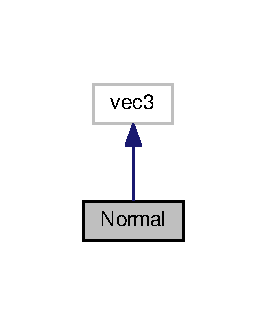
\includegraphics[width=128pt]{struct_normal__inherit__graph}
\end{center}
\end{figure}


Collaboration diagram for Normal\+:
\nopagebreak
\begin{figure}[H]
\begin{center}
\leavevmode
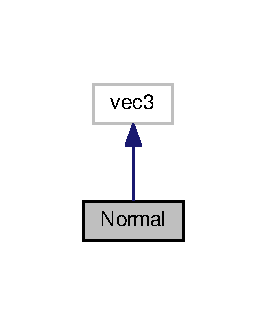
\includegraphics[width=128pt]{struct_normal__coll__graph}
\end{center}
\end{figure}
\subsection*{Public Member Functions}
\begin{DoxyCompactItemize}
\item 
\hyperlink{struct_normal_af62e51ec40dc2eedc3b9ca49ebdc7197}{Normal} ()
\item 
\hyperlink{struct_normal_acf08fa0dafb56ea445b20c882a503292}{Normal} (float x, float y, float z)
\end{DoxyCompactItemize}


\subsection{Detailed Description}


Definition at line 8 of file Normal.\+h.



\subsection{Constructor \& Destructor Documentation}
\mbox{\Hypertarget{struct_normal_af62e51ec40dc2eedc3b9ca49ebdc7197}\label{struct_normal_af62e51ec40dc2eedc3b9ca49ebdc7197}} 
\index{Normal@{Normal}!Normal@{Normal}}
\index{Normal@{Normal}!Normal@{Normal}}
\subsubsection{\texorpdfstring{Normal()}{Normal()}\hspace{0.1cm}{\footnotesize\ttfamily [1/2]}}
{\footnotesize\ttfamily Normal\+::\+Normal (\begin{DoxyParamCaption}{ }\end{DoxyParamCaption})\hspace{0.3cm}{\ttfamily [inline]}}



Definition at line 10 of file Normal.\+h.

\mbox{\Hypertarget{struct_normal_acf08fa0dafb56ea445b20c882a503292}\label{struct_normal_acf08fa0dafb56ea445b20c882a503292}} 
\index{Normal@{Normal}!Normal@{Normal}}
\index{Normal@{Normal}!Normal@{Normal}}
\subsubsection{\texorpdfstring{Normal()}{Normal()}\hspace{0.1cm}{\footnotesize\ttfamily [2/2]}}
{\footnotesize\ttfamily Normal\+::\+Normal (\begin{DoxyParamCaption}\item[{float}]{x,  }\item[{float}]{y,  }\item[{float}]{z }\end{DoxyParamCaption})\hspace{0.3cm}{\ttfamily [inline]}}



Definition at line 11 of file Normal.\+h.



The documentation for this struct was generated from the following file\+:\begin{DoxyCompactItemize}
\item 
/home/rory/\+Projects/ece-\/6122-\/final-\/project/src/objects/\hyperlink{_normal_8h}{Normal.\+h}\end{DoxyCompactItemize}

\hypertarget{class_object}{}\section{Object Class Reference}
\label{class_object}\index{Object@{Object}}


{\ttfamily \#include $<$Object.\+h$>$}

\subsection*{Public Member Functions}
\begin{DoxyCompactItemize}
\item 
\hyperlink{class_object_a8524d31fc25bf997ae127b85ffebe23e}{Object} (const char $\ast$filepath)
\item 
\hyperlink{class_object_ae8f5483f459e46687bd01e6f9977afd3}{$\sim$\+Object} ()
\item 
void \hyperlink{class_object_abcecd0a84919c1abeee1f95044fbf1c1}{submit} (\hyperlink{class_renderer}{Renderer} $\ast$renderer) const
\item 
const std\+::vector$<$ \hyperlink{class_mesh}{Mesh} $>$ \& \hyperlink{class_object_a0c73a3e0bcadac01866e022cbe327082}{get\+Meshes} () const
\item 
const std\+::vector$<$ \hyperlink{class_material}{Material} $>$ \& \hyperlink{class_object_a69844ac34730373cb824a608727fa6ff}{get\+Materials} () const
\item 
const std\+::vector$<$ \hyperlink{struct_position}{Position} $>$ \& \hyperlink{class_object_a7dde4f00d9004f52ddcd12077dbd71b8}{get\+Positions} () const
\item 
std\+::vector$<$ glm\+::vec3 $>$ \hyperlink{class_object_a1d0e144917e58aab0c97e15c796c08dd}{get\+Positions\+Glm\+Vec3} () const
\item 
const std\+::vector$<$ \hyperlink{struct_normal}{Normal} $>$ \& \hyperlink{class_object_afc89c45ef455b9e1fc95d49514d48373}{get\+Normals} () const
\item 
const std\+::vector$<$ \hyperlink{struct_tex_coord}{Tex\+Coord} $>$ \& \hyperlink{class_object_a215c16f0d10edb9d21d41eca96a782d7}{get\+Tex\+Coords} () const
\item 
const glm\+::vec3 \& \hyperlink{class_object_a1054369eab029c63e58de78b88bbd627}{get\+World\+Origin} () const
\item 
const float \& \hyperlink{class_object_a334afec6a91a5c6473d75858771597a2}{get\+Mass} () const
\item 
const glm\+::vec3 \& \hyperlink{class_object_a2d23e6dad9e8c355dda6b3f466d202f3}{get\+Inertia} () const
\item 
const glm\+::vec3 \& \hyperlink{class_object_ac4f74b9b50fb83829b6844a2591ba50f}{get\+Size} () const
\item 
const \hyperlink{struct_position}{Position} $\ast$ \hyperlink{class_object_a247968a9aa55c670e2d462876f5e2cb6}{get\+Position} (unsigned int index) const
\item 
const \hyperlink{struct_normal}{Normal} $\ast$ \hyperlink{class_object_a096f8e6bd78d8f6d31b8897fad9b8e78}{get\+Normal} (unsigned int index) const
\item 
const \hyperlink{struct_tex_coord}{Tex\+Coord} $\ast$ \hyperlink{class_object_a703e8fc9f5aa16d5b657ed8f03f4cf02}{get\+Tex\+Coord} (unsigned int index) const
\item 
int \hyperlink{class_object_acc363689a681f08be8492107ab6ab2f4}{get\+Position\+Index} (\hyperlink{struct_position}{Position} position) const
\item 
int \hyperlink{class_object_a877e446e1e1af8bbe11db702221bc194}{get\+Normal\+Index} (\hyperlink{struct_normal}{Normal} normal) const
\item 
int \hyperlink{class_object_af99105478aba428c8c252598707323b6}{get\+Tex\+Coord\+Index} (\hyperlink{struct_tex_coord}{Tex\+Coord} texcoord) const
\item 
void \hyperlink{class_object_a426314ec1a1e0ae48cbb2b3667c63bb6}{set\+Mass} (const float \&mass)
\item 
void \hyperlink{class_object_a1a82190deb7c8c2da2f3e82562aa7b17}{set\+Inertia} (const glm\+::vec3 \&inertia)
\item 
void \hyperlink{class_object_ac1d7782db71b581a3dd60f25c00bdfd7}{set\+Transform} (glm\+::mat4 transform)
\item 
void \hyperlink{class_object_a1ef8f20019002996c0c62f2b6a38b4f6}{add\+Mesh} (\hyperlink{class_mesh}{Mesh} mesh)
\item 
void \hyperlink{class_object_aa8246a72ca14daf6627b44eaa422c4fb}{add\+Material} (\hyperlink{class_material}{Material} material)
\item 
unsigned int \hyperlink{class_object_aed6fb1a005f657408604c2c2c41e7cd1}{add\+Position} (\hyperlink{struct_position}{Position} position)
\item 
unsigned int \hyperlink{class_object_aeac027a860fad228b5cd3fa4c1a477f8}{add\+Normal} (\hyperlink{struct_normal}{Normal} normal)
\item 
unsigned int \hyperlink{class_object_af978ee81ebe44916aadc434a84fdf1bf}{add\+Tex\+Coord} (\hyperlink{struct_tex_coord}{Tex\+Coord} texcoord)
\end{DoxyCompactItemize}


\subsection{Detailed Description}


Definition at line 13 of file Object.\+h.



\subsection{Constructor \& Destructor Documentation}
\mbox{\Hypertarget{class_object_a8524d31fc25bf997ae127b85ffebe23e}\label{class_object_a8524d31fc25bf997ae127b85ffebe23e}} 
\index{Object@{Object}!Object@{Object}}
\index{Object@{Object}!Object@{Object}}
\subsubsection{\texorpdfstring{Object()}{Object()}}
{\footnotesize\ttfamily Object\+::\+Object (\begin{DoxyParamCaption}\item[{const char $\ast$}]{filepath }\end{DoxyParamCaption})}

Constructor 
\begin{DoxyParams}{Parameters}
{\em filepath} & T\+O\+DO Document \\
\hline
\end{DoxyParams}


Definition at line 17 of file Object.\+cpp.

\mbox{\Hypertarget{class_object_ae8f5483f459e46687bd01e6f9977afd3}\label{class_object_ae8f5483f459e46687bd01e6f9977afd3}} 
\index{Object@{Object}!````~Object@{$\sim$\+Object}}
\index{````~Object@{$\sim$\+Object}!Object@{Object}}
\subsubsection{\texorpdfstring{$\sim$\+Object()}{~Object()}}
{\footnotesize\ttfamily Object\+::$\sim$\+Object (\begin{DoxyParamCaption}{ }\end{DoxyParamCaption})}

Destructor 

Definition at line 49 of file Object.\+cpp.



\subsection{Member Function Documentation}
\mbox{\Hypertarget{class_object_aa8246a72ca14daf6627b44eaa422c4fb}\label{class_object_aa8246a72ca14daf6627b44eaa422c4fb}} 
\index{Object@{Object}!add\+Material@{add\+Material}}
\index{add\+Material@{add\+Material}!Object@{Object}}
\subsubsection{\texorpdfstring{add\+Material()}{addMaterial()}}
{\footnotesize\ttfamily void Object\+::add\+Material (\begin{DoxyParamCaption}\item[{\hyperlink{class_material}{Material}}]{material }\end{DoxyParamCaption})}

T\+O\+DO Document 
\begin{DoxyParams}{Parameters}
{\em position} & T\+O\+DO Document \\
\hline
\end{DoxyParams}


Definition at line 283 of file Object.\+cpp.

\mbox{\Hypertarget{class_object_a1ef8f20019002996c0c62f2b6a38b4f6}\label{class_object_a1ef8f20019002996c0c62f2b6a38b4f6}} 
\index{Object@{Object}!add\+Mesh@{add\+Mesh}}
\index{add\+Mesh@{add\+Mesh}!Object@{Object}}
\subsubsection{\texorpdfstring{add\+Mesh()}{addMesh()}}
{\footnotesize\ttfamily void Object\+::add\+Mesh (\begin{DoxyParamCaption}\item[{\hyperlink{class_mesh}{Mesh}}]{mesh }\end{DoxyParamCaption})}

T\+O\+DO Document 
\begin{DoxyParams}{Parameters}
{\em position} & T\+O\+DO Document \\
\hline
\end{DoxyParams}


Definition at line 274 of file Object.\+cpp.

\mbox{\Hypertarget{class_object_aeac027a860fad228b5cd3fa4c1a477f8}\label{class_object_aeac027a860fad228b5cd3fa4c1a477f8}} 
\index{Object@{Object}!add\+Normal@{add\+Normal}}
\index{add\+Normal@{add\+Normal}!Object@{Object}}
\subsubsection{\texorpdfstring{add\+Normal()}{addNormal()}}
{\footnotesize\ttfamily unsigned int Object\+::add\+Normal (\begin{DoxyParamCaption}\item[{\hyperlink{struct_normal}{Normal}}]{normal }\end{DoxyParamCaption})}

T\+O\+DO Document 
\begin{DoxyParams}{Parameters}
{\em position} & T\+O\+DO Document \\
\hline
\end{DoxyParams}


Definition at line 306 of file Object.\+cpp.

\mbox{\Hypertarget{class_object_aed6fb1a005f657408604c2c2c41e7cd1}\label{class_object_aed6fb1a005f657408604c2c2c41e7cd1}} 
\index{Object@{Object}!add\+Position@{add\+Position}}
\index{add\+Position@{add\+Position}!Object@{Object}}
\subsubsection{\texorpdfstring{add\+Position()}{addPosition()}}
{\footnotesize\ttfamily unsigned int Object\+::add\+Position (\begin{DoxyParamCaption}\item[{\hyperlink{struct_position}{Position}}]{position }\end{DoxyParamCaption})}

T\+O\+DO Document 
\begin{DoxyParams}{Parameters}
{\em position} & T\+O\+DO Document \\
\hline
\end{DoxyParams}


Definition at line 291 of file Object.\+cpp.

\mbox{\Hypertarget{class_object_af978ee81ebe44916aadc434a84fdf1bf}\label{class_object_af978ee81ebe44916aadc434a84fdf1bf}} 
\index{Object@{Object}!add\+Tex\+Coord@{add\+Tex\+Coord}}
\index{add\+Tex\+Coord@{add\+Tex\+Coord}!Object@{Object}}
\subsubsection{\texorpdfstring{add\+Tex\+Coord()}{addTexCoord()}}
{\footnotesize\ttfamily unsigned int Object\+::add\+Tex\+Coord (\begin{DoxyParamCaption}\item[{\hyperlink{struct_tex_coord}{Tex\+Coord}}]{texcoord }\end{DoxyParamCaption})}

T\+O\+DO Document 
\begin{DoxyParams}{Parameters}
{\em position} & T\+O\+DO Document \\
\hline
\end{DoxyParams}


Definition at line 321 of file Object.\+cpp.

\mbox{\Hypertarget{class_object_a2d23e6dad9e8c355dda6b3f466d202f3}\label{class_object_a2d23e6dad9e8c355dda6b3f466d202f3}} 
\index{Object@{Object}!get\+Inertia@{get\+Inertia}}
\index{get\+Inertia@{get\+Inertia}!Object@{Object}}
\subsubsection{\texorpdfstring{get\+Inertia()}{getInertia()}}
{\footnotesize\ttfamily const glm\+::vec3 \& Object\+::get\+Inertia (\begin{DoxyParamCaption}{ }\end{DoxyParamCaption}) const}

T\+O\+DO Document \begin{DoxyReturn}{Returns}
T\+O\+DO Document 
\end{DoxyReturn}


Definition at line 143 of file Object.\+cpp.

\mbox{\Hypertarget{class_object_a334afec6a91a5c6473d75858771597a2}\label{class_object_a334afec6a91a5c6473d75858771597a2}} 
\index{Object@{Object}!get\+Mass@{get\+Mass}}
\index{get\+Mass@{get\+Mass}!Object@{Object}}
\subsubsection{\texorpdfstring{get\+Mass()}{getMass()}}
{\footnotesize\ttfamily const float \& Object\+::get\+Mass (\begin{DoxyParamCaption}{ }\end{DoxyParamCaption}) const}

T\+O\+DO Document \begin{DoxyReturn}{Returns}
T\+O\+DO Document 
\end{DoxyReturn}


Definition at line 134 of file Object.\+cpp.

\mbox{\Hypertarget{class_object_a69844ac34730373cb824a608727fa6ff}\label{class_object_a69844ac34730373cb824a608727fa6ff}} 
\index{Object@{Object}!get\+Materials@{get\+Materials}}
\index{get\+Materials@{get\+Materials}!Object@{Object}}
\subsubsection{\texorpdfstring{get\+Materials()}{getMaterials()}}
{\footnotesize\ttfamily const std\+::vector$<$ \hyperlink{class_material}{Material} $>$ \& Object\+::get\+Materials (\begin{DoxyParamCaption}{ }\end{DoxyParamCaption}) const}

T\+O\+DO Document \begin{DoxyReturn}{Returns}
T\+O\+DO Document 
\end{DoxyReturn}


Definition at line 77 of file Object.\+cpp.

\mbox{\Hypertarget{class_object_a0c73a3e0bcadac01866e022cbe327082}\label{class_object_a0c73a3e0bcadac01866e022cbe327082}} 
\index{Object@{Object}!get\+Meshes@{get\+Meshes}}
\index{get\+Meshes@{get\+Meshes}!Object@{Object}}
\subsubsection{\texorpdfstring{get\+Meshes()}{getMeshes()}}
{\footnotesize\ttfamily const std\+::vector$<$ \hyperlink{class_mesh}{Mesh} $>$ \& Object\+::get\+Meshes (\begin{DoxyParamCaption}{ }\end{DoxyParamCaption}) const}

Get the meshes that make up this object \begin{DoxyReturn}{Returns}
Returns this object\textquotesingle{}s meshes 
\end{DoxyReturn}


Definition at line 68 of file Object.\+cpp.

\mbox{\Hypertarget{class_object_a096f8e6bd78d8f6d31b8897fad9b8e78}\label{class_object_a096f8e6bd78d8f6d31b8897fad9b8e78}} 
\index{Object@{Object}!get\+Normal@{get\+Normal}}
\index{get\+Normal@{get\+Normal}!Object@{Object}}
\subsubsection{\texorpdfstring{get\+Normal()}{getNormal()}}
{\footnotesize\ttfamily const \hyperlink{struct_normal}{Normal} $\ast$ Object\+::get\+Normal (\begin{DoxyParamCaption}\item[{unsigned int}]{index }\end{DoxyParamCaption}) const}

T\+O\+DO Document 
\begin{DoxyParams}{Parameters}
{\em index} & T\+O\+DO Document \\
\hline
\end{DoxyParams}
\begin{DoxyReturn}{Returns}
T\+O\+DO Document 
\end{DoxyReturn}


Definition at line 174 of file Object.\+cpp.

\mbox{\Hypertarget{class_object_a877e446e1e1af8bbe11db702221bc194}\label{class_object_a877e446e1e1af8bbe11db702221bc194}} 
\index{Object@{Object}!get\+Normal\+Index@{get\+Normal\+Index}}
\index{get\+Normal\+Index@{get\+Normal\+Index}!Object@{Object}}
\subsubsection{\texorpdfstring{get\+Normal\+Index()}{getNormalIndex()}}
{\footnotesize\ttfamily int Object\+::get\+Normal\+Index (\begin{DoxyParamCaption}\item[{\hyperlink{struct_normal}{Normal}}]{normal }\end{DoxyParamCaption}) const}

T\+O\+DO Document \begin{DoxyReturn}{Returns}
T\+O\+DO Document 
\end{DoxyReturn}


Definition at line 213 of file Object.\+cpp.

\mbox{\Hypertarget{class_object_afc89c45ef455b9e1fc95d49514d48373}\label{class_object_afc89c45ef455b9e1fc95d49514d48373}} 
\index{Object@{Object}!get\+Normals@{get\+Normals}}
\index{get\+Normals@{get\+Normals}!Object@{Object}}
\subsubsection{\texorpdfstring{get\+Normals()}{getNormals()}}
{\footnotesize\ttfamily const std\+::vector$<$ \hyperlink{struct_normal}{Normal} $>$ \& Object\+::get\+Normals (\begin{DoxyParamCaption}{ }\end{DoxyParamCaption}) const}

T\+O\+DO Document \begin{DoxyReturn}{Returns}
T\+O\+DO Document 
\end{DoxyReturn}


Definition at line 107 of file Object.\+cpp.

\mbox{\Hypertarget{class_object_a247968a9aa55c670e2d462876f5e2cb6}\label{class_object_a247968a9aa55c670e2d462876f5e2cb6}} 
\index{Object@{Object}!get\+Position@{get\+Position}}
\index{get\+Position@{get\+Position}!Object@{Object}}
\subsubsection{\texorpdfstring{get\+Position()}{getPosition()}}
{\footnotesize\ttfamily const \hyperlink{struct_position}{Position} $\ast$ Object\+::get\+Position (\begin{DoxyParamCaption}\item[{unsigned int}]{index }\end{DoxyParamCaption}) const}

T\+O\+DO Document 
\begin{DoxyParams}{Parameters}
{\em index} & T\+O\+DO Document \\
\hline
\end{DoxyParams}
\begin{DoxyReturn}{Returns}
T\+O\+DO Document 
\end{DoxyReturn}


Definition at line 162 of file Object.\+cpp.

\mbox{\Hypertarget{class_object_acc363689a681f08be8492107ab6ab2f4}\label{class_object_acc363689a681f08be8492107ab6ab2f4}} 
\index{Object@{Object}!get\+Position\+Index@{get\+Position\+Index}}
\index{get\+Position\+Index@{get\+Position\+Index}!Object@{Object}}
\subsubsection{\texorpdfstring{get\+Position\+Index()}{getPositionIndex()}}
{\footnotesize\ttfamily int Object\+::get\+Position\+Index (\begin{DoxyParamCaption}\item[{\hyperlink{struct_position}{Position}}]{position }\end{DoxyParamCaption}) const}

T\+O\+DO Document \begin{DoxyReturn}{Returns}
T\+O\+DO Document 
\end{DoxyReturn}


Definition at line 197 of file Object.\+cpp.

\mbox{\Hypertarget{class_object_a7dde4f00d9004f52ddcd12077dbd71b8}\label{class_object_a7dde4f00d9004f52ddcd12077dbd71b8}} 
\index{Object@{Object}!get\+Positions@{get\+Positions}}
\index{get\+Positions@{get\+Positions}!Object@{Object}}
\subsubsection{\texorpdfstring{get\+Positions()}{getPositions()}}
{\footnotesize\ttfamily const std\+::vector$<$ \hyperlink{struct_position}{Position} $>$ \& Object\+::get\+Positions (\begin{DoxyParamCaption}{ }\end{DoxyParamCaption}) const}

T\+O\+DO Document \begin{DoxyReturn}{Returns}
T\+O\+DO Document 
\end{DoxyReturn}


Definition at line 86 of file Object.\+cpp.

\mbox{\Hypertarget{class_object_a1d0e144917e58aab0c97e15c796c08dd}\label{class_object_a1d0e144917e58aab0c97e15c796c08dd}} 
\index{Object@{Object}!get\+Positions\+Glm\+Vec3@{get\+Positions\+Glm\+Vec3}}
\index{get\+Positions\+Glm\+Vec3@{get\+Positions\+Glm\+Vec3}!Object@{Object}}
\subsubsection{\texorpdfstring{get\+Positions\+Glm\+Vec3()}{getPositionsGlmVec3()}}
{\footnotesize\ttfamily std\+::vector$<$ glm\+::vec3 $>$ Object\+::get\+Positions\+Glm\+Vec3 (\begin{DoxyParamCaption}{ }\end{DoxyParamCaption}) const}

T\+O\+DO Document \begin{DoxyReturn}{Returns}
T\+O\+DO Document 
\end{DoxyReturn}


Definition at line 95 of file Object.\+cpp.

\mbox{\Hypertarget{class_object_ac4f74b9b50fb83829b6844a2591ba50f}\label{class_object_ac4f74b9b50fb83829b6844a2591ba50f}} 
\index{Object@{Object}!get\+Size@{get\+Size}}
\index{get\+Size@{get\+Size}!Object@{Object}}
\subsubsection{\texorpdfstring{get\+Size()}{getSize()}}
{\footnotesize\ttfamily const glm\+::vec3 \& Object\+::get\+Size (\begin{DoxyParamCaption}{ }\end{DoxyParamCaption}) const}

T\+O\+DO Document \begin{DoxyReturn}{Returns}
T\+O\+DO Document 
\end{DoxyReturn}


Definition at line 152 of file Object.\+cpp.

\mbox{\Hypertarget{class_object_a703e8fc9f5aa16d5b657ed8f03f4cf02}\label{class_object_a703e8fc9f5aa16d5b657ed8f03f4cf02}} 
\index{Object@{Object}!get\+Tex\+Coord@{get\+Tex\+Coord}}
\index{get\+Tex\+Coord@{get\+Tex\+Coord}!Object@{Object}}
\subsubsection{\texorpdfstring{get\+Tex\+Coord()}{getTexCoord()}}
{\footnotesize\ttfamily const \hyperlink{struct_tex_coord}{Tex\+Coord} $\ast$ Object\+::get\+Tex\+Coord (\begin{DoxyParamCaption}\item[{unsigned int}]{index }\end{DoxyParamCaption}) const}

T\+O\+DO Document 
\begin{DoxyParams}{Parameters}
{\em index} & T\+O\+DO Document \\
\hline
\end{DoxyParams}
\begin{DoxyReturn}{Returns}
T\+O\+DO Document 
\end{DoxyReturn}


Definition at line 186 of file Object.\+cpp.

\mbox{\Hypertarget{class_object_af99105478aba428c8c252598707323b6}\label{class_object_af99105478aba428c8c252598707323b6}} 
\index{Object@{Object}!get\+Tex\+Coord\+Index@{get\+Tex\+Coord\+Index}}
\index{get\+Tex\+Coord\+Index@{get\+Tex\+Coord\+Index}!Object@{Object}}
\subsubsection{\texorpdfstring{get\+Tex\+Coord\+Index()}{getTexCoordIndex()}}
{\footnotesize\ttfamily int Object\+::get\+Tex\+Coord\+Index (\begin{DoxyParamCaption}\item[{\hyperlink{struct_tex_coord}{Tex\+Coord}}]{texcoord }\end{DoxyParamCaption}) const}

T\+O\+DO Document \begin{DoxyReturn}{Returns}
T\+O\+DO Document 
\end{DoxyReturn}


Definition at line 229 of file Object.\+cpp.

\mbox{\Hypertarget{class_object_a215c16f0d10edb9d21d41eca96a782d7}\label{class_object_a215c16f0d10edb9d21d41eca96a782d7}} 
\index{Object@{Object}!get\+Tex\+Coords@{get\+Tex\+Coords}}
\index{get\+Tex\+Coords@{get\+Tex\+Coords}!Object@{Object}}
\subsubsection{\texorpdfstring{get\+Tex\+Coords()}{getTexCoords()}}
{\footnotesize\ttfamily const std\+::vector$<$ \hyperlink{struct_tex_coord}{Tex\+Coord} $>$ \& Object\+::get\+Tex\+Coords (\begin{DoxyParamCaption}{ }\end{DoxyParamCaption}) const}

T\+O\+DO Document \begin{DoxyReturn}{Returns}
T\+O\+DO Document 
\end{DoxyReturn}


Definition at line 116 of file Object.\+cpp.

\mbox{\Hypertarget{class_object_a1054369eab029c63e58de78b88bbd627}\label{class_object_a1054369eab029c63e58de78b88bbd627}} 
\index{Object@{Object}!get\+World\+Origin@{get\+World\+Origin}}
\index{get\+World\+Origin@{get\+World\+Origin}!Object@{Object}}
\subsubsection{\texorpdfstring{get\+World\+Origin()}{getWorldOrigin()}}
{\footnotesize\ttfamily const glm\+::vec3 \& Object\+::get\+World\+Origin (\begin{DoxyParamCaption}{ }\end{DoxyParamCaption}) const}

T\+O\+DO Document \begin{DoxyReturn}{Returns}
T\+O\+DO Document 
\end{DoxyReturn}


Definition at line 125 of file Object.\+cpp.

\mbox{\Hypertarget{class_object_a1a82190deb7c8c2da2f3e82562aa7b17}\label{class_object_a1a82190deb7c8c2da2f3e82562aa7b17}} 
\index{Object@{Object}!set\+Inertia@{set\+Inertia}}
\index{set\+Inertia@{set\+Inertia}!Object@{Object}}
\subsubsection{\texorpdfstring{set\+Inertia()}{setInertia()}}
{\footnotesize\ttfamily void Object\+::set\+Inertia (\begin{DoxyParamCaption}\item[{const glm\+::vec3 \&}]{inertia }\end{DoxyParamCaption})}

T\+O\+DO Document \begin{DoxyReturn}{Returns}
T\+O\+DO Document 
\end{DoxyReturn}


Definition at line 253 of file Object.\+cpp.

\mbox{\Hypertarget{class_object_a426314ec1a1e0ae48cbb2b3667c63bb6}\label{class_object_a426314ec1a1e0ae48cbb2b3667c63bb6}} 
\index{Object@{Object}!set\+Mass@{set\+Mass}}
\index{set\+Mass@{set\+Mass}!Object@{Object}}
\subsubsection{\texorpdfstring{set\+Mass()}{setMass()}}
{\footnotesize\ttfamily void Object\+::set\+Mass (\begin{DoxyParamCaption}\item[{const float \&}]{mass }\end{DoxyParamCaption})}

T\+O\+DO Document \begin{DoxyReturn}{Returns}
T\+O\+DO Document 
\end{DoxyReturn}


Definition at line 244 of file Object.\+cpp.

\mbox{\Hypertarget{class_object_ac1d7782db71b581a3dd60f25c00bdfd7}\label{class_object_ac1d7782db71b581a3dd60f25c00bdfd7}} 
\index{Object@{Object}!set\+Transform@{set\+Transform}}
\index{set\+Transform@{set\+Transform}!Object@{Object}}
\subsubsection{\texorpdfstring{set\+Transform()}{setTransform()}}
{\footnotesize\ttfamily void Object\+::set\+Transform (\begin{DoxyParamCaption}\item[{glm\+::mat4}]{transform }\end{DoxyParamCaption})}

T\+O\+DO Document 
\begin{DoxyParams}{Parameters}
{\em transform} & T\+O\+DO Document \\
\hline
\end{DoxyParams}


Definition at line 262 of file Object.\+cpp.

\mbox{\Hypertarget{class_object_abcecd0a84919c1abeee1f95044fbf1c1}\label{class_object_abcecd0a84919c1abeee1f95044fbf1c1}} 
\index{Object@{Object}!submit@{submit}}
\index{submit@{submit}!Object@{Object}}
\subsubsection{\texorpdfstring{submit()}{submit()}}
{\footnotesize\ttfamily void Object\+::submit (\begin{DoxyParamCaption}\item[{\hyperlink{class_renderer}{Renderer} $\ast$}]{renderer }\end{DoxyParamCaption}) const}

This function simply submits this shape to its renderer. It is up to the renderer to actually draw it 
\begin{DoxyParams}{Parameters}
{\em renderer} & The renderer to use for drawing \\
\hline
\end{DoxyParams}


Definition at line 59 of file Object.\+cpp.



The documentation for this class was generated from the following files\+:\begin{DoxyCompactItemize}
\item 
/home/rory/\+Projects/ece-\/6122-\/final-\/project/src/objects/\hyperlink{_object_8h}{Object.\+h}\item 
/home/rory/\+Projects/ece-\/6122-\/final-\/project/src/objects/\hyperlink{_object_8cpp}{Object.\+cpp}\end{DoxyCompactItemize}

\hypertarget{class_object_loader}{}\section{Object\+Loader Class Reference}
\label{class_object_loader}\index{Object\+Loader@{Object\+Loader}}


{\ttfamily \#include $<$Object\+Loader.\+h$>$}

\subsection*{Static Public Member Functions}
\begin{DoxyCompactItemize}
\item 
static void \hyperlink{class_object_loader_a1d0581ac5b2ee9e239b68ea6d4875153}{load\+From\+File} (const char $\ast$filepath, \hyperlink{class_object}{Object} $\ast$object)
\end{DoxyCompactItemize}


\subsection{Detailed Description}


Definition at line 9 of file Object\+Loader.\+h.



\subsection{Member Function Documentation}
\mbox{\Hypertarget{class_object_loader_a1d0581ac5b2ee9e239b68ea6d4875153}\label{class_object_loader_a1d0581ac5b2ee9e239b68ea6d4875153}} 
\index{Object\+Loader@{Object\+Loader}!load\+From\+File@{load\+From\+File}}
\index{load\+From\+File@{load\+From\+File}!Object\+Loader@{Object\+Loader}}
\subsubsection{\texorpdfstring{load\+From\+File()}{loadFromFile()}}
{\footnotesize\ttfamily void Object\+Loader\+::load\+From\+File (\begin{DoxyParamCaption}\item[{const char $\ast$}]{filepath,  }\item[{\hyperlink{class_object}{Object} $\ast$}]{object }\end{DoxyParamCaption})\hspace{0.3cm}{\ttfamily [static]}}

T\+O\+DO 
\begin{DoxyParams}{Parameters}
{\em filepath} & T\+O\+DO \\
\hline
\end{DoxyParams}
\begin{DoxyReturn}{Returns}
T\+O\+DO 
\end{DoxyReturn}


Definition at line 25 of file Object\+Loader.\+cpp.



The documentation for this class was generated from the following files\+:\begin{DoxyCompactItemize}
\item 
/home/rory/\+Projects/ece-\/6122-\/final-\/project/src/objects/\hyperlink{_object_loader_8h}{Object\+Loader.\+h}\item 
/home/rory/\+Projects/ece-\/6122-\/final-\/project/src/objects/\hyperlink{_object_loader_8cpp}{Object\+Loader.\+cpp}\end{DoxyCompactItemize}

\hypertarget{structobj_metadata}{}\section{obj\+Metadata Struct Reference}
\label{structobj_metadata}\index{obj\+Metadata@{obj\+Metadata}}
\subsection*{Public Attributes}
\begin{DoxyCompactItemize}
\item 
\hyperlink{main_8cpp_a5a4538eeab397888d88a4eefcc5a1345}{Shape\+Type} \hyperlink{structobj_metadata_af6153058d69f26848a28eeae724d8f05}{type}
\item 
glm\+::vec3 \hyperlink{structobj_metadata_aa08b002e6a99770d0c68e03ab25088ff}{position}
\item 
float \hyperlink{structobj_metadata_ac2df1bad1e332a30af67e57a55a93930}{mass}
\item 
float \hyperlink{structobj_metadata_ad38eef7c4699d2a74423f2e0d8ef8559}{bounciness}
\item 
float \hyperlink{structobj_metadata_a672e831325e522dd8fe5eecbab6a6f94}{friction}
\item 
const char $\ast$ \hyperlink{structobj_metadata_a7e922e759ce7c08f2f70c47034b1880a}{filepath}
\end{DoxyCompactItemize}


\subsection{Detailed Description}


Definition at line 33 of file main.\+cpp.



\subsection{Member Data Documentation}
\mbox{\Hypertarget{structobj_metadata_ad38eef7c4699d2a74423f2e0d8ef8559}\label{structobj_metadata_ad38eef7c4699d2a74423f2e0d8ef8559}} 
\index{obj\+Metadata@{obj\+Metadata}!bounciness@{bounciness}}
\index{bounciness@{bounciness}!obj\+Metadata@{obj\+Metadata}}
\subsubsection{\texorpdfstring{bounciness}{bounciness}}
{\footnotesize\ttfamily float obj\+Metadata\+::bounciness}



Definition at line 38 of file main.\+cpp.

\mbox{\Hypertarget{structobj_metadata_a7e922e759ce7c08f2f70c47034b1880a}\label{structobj_metadata_a7e922e759ce7c08f2f70c47034b1880a}} 
\index{obj\+Metadata@{obj\+Metadata}!filepath@{filepath}}
\index{filepath@{filepath}!obj\+Metadata@{obj\+Metadata}}
\subsubsection{\texorpdfstring{filepath}{filepath}}
{\footnotesize\ttfamily const char$\ast$ obj\+Metadata\+::filepath}



Definition at line 40 of file main.\+cpp.

\mbox{\Hypertarget{structobj_metadata_a672e831325e522dd8fe5eecbab6a6f94}\label{structobj_metadata_a672e831325e522dd8fe5eecbab6a6f94}} 
\index{obj\+Metadata@{obj\+Metadata}!friction@{friction}}
\index{friction@{friction}!obj\+Metadata@{obj\+Metadata}}
\subsubsection{\texorpdfstring{friction}{friction}}
{\footnotesize\ttfamily float obj\+Metadata\+::friction}



Definition at line 39 of file main.\+cpp.

\mbox{\Hypertarget{structobj_metadata_ac2df1bad1e332a30af67e57a55a93930}\label{structobj_metadata_ac2df1bad1e332a30af67e57a55a93930}} 
\index{obj\+Metadata@{obj\+Metadata}!mass@{mass}}
\index{mass@{mass}!obj\+Metadata@{obj\+Metadata}}
\subsubsection{\texorpdfstring{mass}{mass}}
{\footnotesize\ttfamily float obj\+Metadata\+::mass}



Definition at line 37 of file main.\+cpp.

\mbox{\Hypertarget{structobj_metadata_aa08b002e6a99770d0c68e03ab25088ff}\label{structobj_metadata_aa08b002e6a99770d0c68e03ab25088ff}} 
\index{obj\+Metadata@{obj\+Metadata}!position@{position}}
\index{position@{position}!obj\+Metadata@{obj\+Metadata}}
\subsubsection{\texorpdfstring{position}{position}}
{\footnotesize\ttfamily glm\+::vec3 obj\+Metadata\+::position}



Definition at line 36 of file main.\+cpp.

\mbox{\Hypertarget{structobj_metadata_af6153058d69f26848a28eeae724d8f05}\label{structobj_metadata_af6153058d69f26848a28eeae724d8f05}} 
\index{obj\+Metadata@{obj\+Metadata}!type@{type}}
\index{type@{type}!obj\+Metadata@{obj\+Metadata}}
\subsubsection{\texorpdfstring{type}{type}}
{\footnotesize\ttfamily \hyperlink{main_8cpp_a5a4538eeab397888d88a4eefcc5a1345}{Shape\+Type} obj\+Metadata\+::type}



Definition at line 35 of file main.\+cpp.



The documentation for this struct was generated from the following file\+:\begin{DoxyCompactItemize}
\item 
/home/rory/\+Projects/ece-\/6122-\/final-\/project/src/\hyperlink{main_8cpp}{main.\+cpp}\end{DoxyCompactItemize}

\hypertarget{class_performance_data}{}\section{Performance\+Data Class Reference}
\label{class_performance_data}\index{Performance\+Data@{Performance\+Data}}


{\ttfamily \#include $<$Performance\+Data.\+h$>$}

\subsection*{Public Member Functions}
\begin{DoxyCompactItemize}
\item 
\hyperlink{class_performance_data_a7766088fec48f94afcf784c027e0ee5d}{Performance\+Data} ()
\item 
void \hyperlink{class_performance_data_ac852244b141ba327f30da7a5fd586d49}{increment\+Frames} ()
\item 
const unsigned int \& \hyperlink{class_performance_data_a9ffcce90095cc9614f88b6ac25ff129d}{get\+Frames} () const
\item 
void \hyperlink{class_performance_data_a622d01a9d885596c79a799f03676c990}{update\+Stats} ()
\item 
void \hyperlink{class_performance_data_a5a19e35de26351c6983f069d25ec5a95}{reset} ()
\item 
double \hyperlink{class_performance_data_a54bcba973a7989024433e6d905140362}{get\+Elapsed\+Time} ()
\item 
double \hyperlink{class_performance_data_a803d0b8ed600dff6100c8c486c599527}{get\+Elapsed\+Time\+Since\+Creation} ()
\item 
const char $\ast$ \hyperlink{class_performance_data_a9f96571086d202296dd4bc3d799b4ac0}{get\+Frames\+Str} () const
\item 
const char $\ast$ \hyperlink{class_performance_data_a083aeabd3aa06b3420b2afdbc6e0e3d1}{get\+Elapsed\+Str} () const
\item 
const char $\ast$ \hyperlink{class_performance_data_aa30d1d2ea4889a3cacc726e4487c7b78}{get\+Fps\+Str} () const
\end{DoxyCompactItemize}


\subsection{Detailed Description}


Definition at line 8 of file Performance\+Data.\+h.



\subsection{Constructor \& Destructor Documentation}
\mbox{\Hypertarget{class_performance_data_a7766088fec48f94afcf784c027e0ee5d}\label{class_performance_data_a7766088fec48f94afcf784c027e0ee5d}} 
\index{Performance\+Data@{Performance\+Data}!Performance\+Data@{Performance\+Data}}
\index{Performance\+Data@{Performance\+Data}!Performance\+Data@{Performance\+Data}}
\subsubsection{\texorpdfstring{Performance\+Data()}{PerformanceData()}}
{\footnotesize\ttfamily Performance\+Data\+::\+Performance\+Data (\begin{DoxyParamCaption}{ }\end{DoxyParamCaption})}

Constructor 

Definition at line 9 of file Performance\+Data.\+cpp.



\subsection{Member Function Documentation}
\mbox{\Hypertarget{class_performance_data_a083aeabd3aa06b3420b2afdbc6e0e3d1}\label{class_performance_data_a083aeabd3aa06b3420b2afdbc6e0e3d1}} 
\index{Performance\+Data@{Performance\+Data}!get\+Elapsed\+Str@{get\+Elapsed\+Str}}
\index{get\+Elapsed\+Str@{get\+Elapsed\+Str}!Performance\+Data@{Performance\+Data}}
\subsubsection{\texorpdfstring{get\+Elapsed\+Str()}{getElapsedStr()}}
{\footnotesize\ttfamily const char $\ast$ Performance\+Data\+::get\+Elapsed\+Str (\begin{DoxyParamCaption}{ }\end{DoxyParamCaption}) const}

Returns the string of the elapsed time since creation \begin{DoxyReturn}{Returns}
Returns the elapsed time since creation string 
\end{DoxyReturn}


Definition at line 130 of file Performance\+Data.\+cpp.

\mbox{\Hypertarget{class_performance_data_a54bcba973a7989024433e6d905140362}\label{class_performance_data_a54bcba973a7989024433e6d905140362}} 
\index{Performance\+Data@{Performance\+Data}!get\+Elapsed\+Time@{get\+Elapsed\+Time}}
\index{get\+Elapsed\+Time@{get\+Elapsed\+Time}!Performance\+Data@{Performance\+Data}}
\subsubsection{\texorpdfstring{get\+Elapsed\+Time()}{getElapsedTime()}}
{\footnotesize\ttfamily double Performance\+Data\+::get\+Elapsed\+Time (\begin{DoxyParamCaption}{ }\end{DoxyParamCaption})}

Updates the current timestamp and returns the elapsed time since \hyperlink{class_performance_data_a5a19e35de26351c6983f069d25ec5a95}{reset()} was called \begin{DoxyReturn}{Returns}
Returns the elapsed time in seconds since \hyperlink{class_performance_data_a5a19e35de26351c6983f069d25ec5a95}{reset()} 
\end{DoxyReturn}


Definition at line 83 of file Performance\+Data.\+cpp.

\mbox{\Hypertarget{class_performance_data_a803d0b8ed600dff6100c8c486c599527}\label{class_performance_data_a803d0b8ed600dff6100c8c486c599527}} 
\index{Performance\+Data@{Performance\+Data}!get\+Elapsed\+Time\+Since\+Creation@{get\+Elapsed\+Time\+Since\+Creation}}
\index{get\+Elapsed\+Time\+Since\+Creation@{get\+Elapsed\+Time\+Since\+Creation}!Performance\+Data@{Performance\+Data}}
\subsubsection{\texorpdfstring{get\+Elapsed\+Time\+Since\+Creation()}{getElapsedTimeSinceCreation()}}
{\footnotesize\ttfamily double Performance\+Data\+::get\+Elapsed\+Time\+Since\+Creation (\begin{DoxyParamCaption}{ }\end{DoxyParamCaption})}

Updates the current timestamp and returns the elapsed time since class creation was called \begin{DoxyReturn}{Returns}
Returns the elapsed time in seconds since class creation 
\end{DoxyReturn}


Definition at line 94 of file Performance\+Data.\+cpp.

\mbox{\Hypertarget{class_performance_data_aa30d1d2ea4889a3cacc726e4487c7b78}\label{class_performance_data_aa30d1d2ea4889a3cacc726e4487c7b78}} 
\index{Performance\+Data@{Performance\+Data}!get\+Fps\+Str@{get\+Fps\+Str}}
\index{get\+Fps\+Str@{get\+Fps\+Str}!Performance\+Data@{Performance\+Data}}
\subsubsection{\texorpdfstring{get\+Fps\+Str()}{getFpsStr()}}
{\footnotesize\ttfamily const char $\ast$ Performance\+Data\+::get\+Fps\+Str (\begin{DoxyParamCaption}{ }\end{DoxyParamCaption}) const}

Returns the string of the frames per second since the last time \hyperlink{class_performance_data_a622d01a9d885596c79a799f03676c990}{update\+Stats()} was called \begin{DoxyReturn}{Returns}
Returns the frames per second string 
\end{DoxyReturn}


Definition at line 140 of file Performance\+Data.\+cpp.

\mbox{\Hypertarget{class_performance_data_a9ffcce90095cc9614f88b6ac25ff129d}\label{class_performance_data_a9ffcce90095cc9614f88b6ac25ff129d}} 
\index{Performance\+Data@{Performance\+Data}!get\+Frames@{get\+Frames}}
\index{get\+Frames@{get\+Frames}!Performance\+Data@{Performance\+Data}}
\subsubsection{\texorpdfstring{get\+Frames()}{getFrames()}}
{\footnotesize\ttfamily const unsigned int \& Performance\+Data\+::get\+Frames (\begin{DoxyParamCaption}{ }\end{DoxyParamCaption}) const}

Return the number of frames \begin{DoxyReturn}{Returns}
Return the number of frames 
\end{DoxyReturn}


Definition at line 63 of file Performance\+Data.\+cpp.

\mbox{\Hypertarget{class_performance_data_a9f96571086d202296dd4bc3d799b4ac0}\label{class_performance_data_a9f96571086d202296dd4bc3d799b4ac0}} 
\index{Performance\+Data@{Performance\+Data}!get\+Frames\+Str@{get\+Frames\+Str}}
\index{get\+Frames\+Str@{get\+Frames\+Str}!Performance\+Data@{Performance\+Data}}
\subsubsection{\texorpdfstring{get\+Frames\+Str()}{getFramesStr()}}
{\footnotesize\ttfamily const char $\ast$ Performance\+Data\+::get\+Frames\+Str (\begin{DoxyParamCaption}{ }\end{DoxyParamCaption}) const}

Returns the string of the frame counter since the last time \hyperlink{class_performance_data_a622d01a9d885596c79a799f03676c990}{update\+Stats()} was called \begin{DoxyReturn}{Returns}

\end{DoxyReturn}


Definition at line 121 of file Performance\+Data.\+cpp.

\mbox{\Hypertarget{class_performance_data_ac852244b141ba327f30da7a5fd586d49}\label{class_performance_data_ac852244b141ba327f30da7a5fd586d49}} 
\index{Performance\+Data@{Performance\+Data}!increment\+Frames@{increment\+Frames}}
\index{increment\+Frames@{increment\+Frames}!Performance\+Data@{Performance\+Data}}
\subsubsection{\texorpdfstring{increment\+Frames()}{incrementFrames()}}
{\footnotesize\ttfamily void Performance\+Data\+::increment\+Frames (\begin{DoxyParamCaption}{ }\end{DoxyParamCaption})}

Increment the frames counter 

Definition at line 54 of file Performance\+Data.\+cpp.

\mbox{\Hypertarget{class_performance_data_a5a19e35de26351c6983f069d25ec5a95}\label{class_performance_data_a5a19e35de26351c6983f069d25ec5a95}} 
\index{Performance\+Data@{Performance\+Data}!reset@{reset}}
\index{reset@{reset}!Performance\+Data@{Performance\+Data}}
\subsubsection{\texorpdfstring{reset()}{reset()}}
{\footnotesize\ttfamily void Performance\+Data\+::reset (\begin{DoxyParamCaption}{ }\end{DoxyParamCaption})}

Resets the performance counters 

Definition at line 71 of file Performance\+Data.\+cpp.

\mbox{\Hypertarget{class_performance_data_a622d01a9d885596c79a799f03676c990}\label{class_performance_data_a622d01a9d885596c79a799f03676c990}} 
\index{Performance\+Data@{Performance\+Data}!update\+Stats@{update\+Stats}}
\index{update\+Stats@{update\+Stats}!Performance\+Data@{Performance\+Data}}
\subsubsection{\texorpdfstring{update\+Stats()}{updateStats()}}
{\footnotesize\ttfamily void Performance\+Data\+::update\+Stats (\begin{DoxyParamCaption}{ }\end{DoxyParamCaption})}

Set all the performance statistics 

Definition at line 103 of file Performance\+Data.\+cpp.



The documentation for this class was generated from the following files\+:\begin{DoxyCompactItemize}
\item 
/home/rory/\+Projects/ece-\/6122-\/final-\/project/src/\hyperlink{_performance_data_8h}{Performance\+Data.\+h}\item 
/home/rory/\+Projects/ece-\/6122-\/final-\/project/src/\hyperlink{_performance_data_8cpp}{Performance\+Data.\+cpp}\end{DoxyCompactItemize}

\hypertarget{class_physics_engine}{}\section{Physics\+Engine Class Reference}
\label{class_physics_engine}\index{Physics\+Engine@{Physics\+Engine}}


{\ttfamily \#include $<$Physics\+Engine.\+h$>$}

\subsection*{Public Member Functions}
\begin{DoxyCompactItemize}
\item 
\hyperlink{class_physics_engine_a7fc9180ea453680df0b863fa157c5b92}{Physics\+Engine} ()
\item 
\hyperlink{class_physics_engine_ae5f076ee99bbfdbc79ab2d27366d8476}{$\sim$\+Physics\+Engine} ()
\item 
void \hyperlink{class_physics_engine_ac9895c911f76466da7a7980d72cf9b08}{step\+Simulation} (const double \&delta\+Time)
\item 
void \hyperlink{class_physics_engine_a1ffbe330ee66c22fde2a8516dc9fc84e}{add\+Sphere} (float radius, float mass, float bounciness, float friction, glm\+::vec3 position)
\item 
void \hyperlink{class_physics_engine_a31a8857189ef80c1dc65a09298dcb9bf}{add\+Box} (glm\+::vec3 size, float mass, float bounciness, float friction, glm\+::vec3 position)
\item 
void \hyperlink{class_physics_engine_ad5e3e5508a2bf990241ad8d12e65e8b6}{add\+Hull} (std\+::vector$<$ glm\+::vec3 $>$ points, float mass, float bounciness, float friction, glm\+::vec3 position)
\item 
void \hyperlink{class_physics_engine_ae51b6b3b006443af2dfd8a2c3ee503bb}{add\+Wall} ()
\item 
void \hyperlink{class_physics_engine_a89715c2d36c8ab11960c5c1effe3ff57}{get\+Motion\+States} (std\+::vector$<$ glm\+::vec3 $>$ \&states)
\item 
void \hyperlink{class_physics_engine_af272bdb214ae594852c8457e45e2b7e3}{get\+Open\+G\+L\+Matrix} (int index, glm\+::mat4 \&matrix)
\end{DoxyCompactItemize}
\subsection*{Static Public Member Functions}
\begin{DoxyCompactItemize}
\item 
static void \hyperlink{class_physics_engine_a78f7f38916d7781c79b7818658c4619a}{simple\+\_\+ball\+\_\+drop} ()
\end{DoxyCompactItemize}


\subsection{Detailed Description}


Definition at line 14 of file Physics\+Engine.\+h.



\subsection{Constructor \& Destructor Documentation}
\mbox{\Hypertarget{class_physics_engine_a7fc9180ea453680df0b863fa157c5b92}\label{class_physics_engine_a7fc9180ea453680df0b863fa157c5b92}} 
\index{Physics\+Engine@{Physics\+Engine}!Physics\+Engine@{Physics\+Engine}}
\index{Physics\+Engine@{Physics\+Engine}!Physics\+Engine@{Physics\+Engine}}
\subsubsection{\texorpdfstring{Physics\+Engine()}{PhysicsEngine()}}
{\footnotesize\ttfamily Physics\+Engine\+::\+Physics\+Engine (\begin{DoxyParamCaption}{ }\end{DoxyParamCaption})}

Constructor 

Definition at line 20 of file Physics\+Engine.\+cpp.

\mbox{\Hypertarget{class_physics_engine_ae5f076ee99bbfdbc79ab2d27366d8476}\label{class_physics_engine_ae5f076ee99bbfdbc79ab2d27366d8476}} 
\index{Physics\+Engine@{Physics\+Engine}!````~Physics\+Engine@{$\sim$\+Physics\+Engine}}
\index{````~Physics\+Engine@{$\sim$\+Physics\+Engine}!Physics\+Engine@{Physics\+Engine}}
\subsubsection{\texorpdfstring{$\sim$\+Physics\+Engine()}{~PhysicsEngine()}}
{\footnotesize\ttfamily Physics\+Engine\+::$\sim$\+Physics\+Engine (\begin{DoxyParamCaption}{ }\end{DoxyParamCaption})}

Destructor 

Definition at line 65 of file Physics\+Engine.\+cpp.



\subsection{Member Function Documentation}
\mbox{\Hypertarget{class_physics_engine_a31a8857189ef80c1dc65a09298dcb9bf}\label{class_physics_engine_a31a8857189ef80c1dc65a09298dcb9bf}} 
\index{Physics\+Engine@{Physics\+Engine}!add\+Box@{add\+Box}}
\index{add\+Box@{add\+Box}!Physics\+Engine@{Physics\+Engine}}
\subsubsection{\texorpdfstring{add\+Box()}{addBox()}}
{\footnotesize\ttfamily void Physics\+Engine\+::add\+Box (\begin{DoxyParamCaption}\item[{glm\+::vec3}]{size,  }\item[{float}]{mass,  }\item[{float}]{bounciness,  }\item[{float}]{friction,  }\item[{glm\+::vec3}]{position }\end{DoxyParamCaption})}

Adds a box to the physics engine 
\begin{DoxyParams}{Parameters}
{\em size} & The size of the box as measured from the origin \\
\hline
{\em mass} & The box\textquotesingle{}s mass \\
\hline
{\em bounciness} & The sphere\textquotesingle{}s bounciness from 0=none to 1=bouncy \\
\hline
{\em friction} & The sphere\textquotesingle{}s friction coefficient from 0=low to 1=high \href{https://www.thoughtspike.com/friction-coefficients-for-bullet-physics/}{\tt https\+://www.\+thoughtspike.\+com/friction-\/coefficients-\/for-\/bullet-\/physics/} \\
\hline
{\em position} & The box\textquotesingle{}s initial position as measured by the origin \\
\hline
\end{DoxyParams}


Definition at line 143 of file Physics\+Engine.\+cpp.

\mbox{\Hypertarget{class_physics_engine_ad5e3e5508a2bf990241ad8d12e65e8b6}\label{class_physics_engine_ad5e3e5508a2bf990241ad8d12e65e8b6}} 
\index{Physics\+Engine@{Physics\+Engine}!add\+Hull@{add\+Hull}}
\index{add\+Hull@{add\+Hull}!Physics\+Engine@{Physics\+Engine}}
\subsubsection{\texorpdfstring{add\+Hull()}{addHull()}}
{\footnotesize\ttfamily void Physics\+Engine\+::add\+Hull (\begin{DoxyParamCaption}\item[{std\+::vector$<$ glm\+::vec3 $>$}]{points,  }\item[{float}]{mass,  }\item[{float}]{bounciness,  }\item[{float}]{friction,  }\item[{glm\+::vec3}]{position }\end{DoxyParamCaption})}

Add a convex hull shape to the physics engine 
\begin{DoxyParams}{Parameters}
{\em points} & T\+O\+DO Document \\
\hline
{\em mass} & T\+O\+DO Document \\
\hline
{\em bounciness} & T\+O\+DO Document \\
\hline
{\em friction} & T\+O\+DO Document \\
\hline
{\em position} & T\+O\+DO Document \\
\hline
\end{DoxyParams}


Definition at line 172 of file Physics\+Engine.\+cpp.

\mbox{\Hypertarget{class_physics_engine_a1ffbe330ee66c22fde2a8516dc9fc84e}\label{class_physics_engine_a1ffbe330ee66c22fde2a8516dc9fc84e}} 
\index{Physics\+Engine@{Physics\+Engine}!add\+Sphere@{add\+Sphere}}
\index{add\+Sphere@{add\+Sphere}!Physics\+Engine@{Physics\+Engine}}
\subsubsection{\texorpdfstring{add\+Sphere()}{addSphere()}}
{\footnotesize\ttfamily void Physics\+Engine\+::add\+Sphere (\begin{DoxyParamCaption}\item[{float}]{radius,  }\item[{float}]{mass,  }\item[{float}]{bounciness,  }\item[{float}]{friction,  }\item[{glm\+::vec3}]{position }\end{DoxyParamCaption})}

Adds a sphere to the physics engine 
\begin{DoxyParams}{Parameters}
{\em radius} & The radius of the sphere \\
\hline
{\em mass} & The sphere\textquotesingle{}s mass \\
\hline
{\em bounciness} & The sphere\textquotesingle{}s bounciness from 0=none to 1=bouncy \\
\hline
{\em friction} & The sphere\textquotesingle{}s friction coefficient from 0=low to 1=high \href{https://www.thoughtspike.com/friction-coefficients-for-bullet-physics/}{\tt https\+://www.\+thoughtspike.\+com/friction-\/coefficients-\/for-\/bullet-\/physics/} \\
\hline
{\em position} & The sphere\textquotesingle{}s initial position as measured from the origin \\
\hline
\end{DoxyParams}


Definition at line 113 of file Physics\+Engine.\+cpp.

\mbox{\Hypertarget{class_physics_engine_ae51b6b3b006443af2dfd8a2c3ee503bb}\label{class_physics_engine_ae51b6b3b006443af2dfd8a2c3ee503bb}} 
\index{Physics\+Engine@{Physics\+Engine}!add\+Wall@{add\+Wall}}
\index{add\+Wall@{add\+Wall}!Physics\+Engine@{Physics\+Engine}}
\subsubsection{\texorpdfstring{add\+Wall()}{addWall()}}
{\footnotesize\ttfamily void Physics\+Engine\+::add\+Wall (\begin{DoxyParamCaption}{ }\end{DoxyParamCaption})}

Add a wall (plane) to the physics engine 

Definition at line 197 of file Physics\+Engine.\+cpp.

\mbox{\Hypertarget{class_physics_engine_a89715c2d36c8ab11960c5c1effe3ff57}\label{class_physics_engine_a89715c2d36c8ab11960c5c1effe3ff57}} 
\index{Physics\+Engine@{Physics\+Engine}!get\+Motion\+States@{get\+Motion\+States}}
\index{get\+Motion\+States@{get\+Motion\+States}!Physics\+Engine@{Physics\+Engine}}
\subsubsection{\texorpdfstring{get\+Motion\+States()}{getMotionStates()}}
{\footnotesize\ttfamily void Physics\+Engine\+::get\+Motion\+States (\begin{DoxyParamCaption}\item[{std\+::vector$<$ glm\+::vec3 $>$ \&}]{states }\end{DoxyParamCaption})}

T\+O\+DO Document 
\begin{DoxyParams}{Parameters}
{\em states} & T\+O\+DO Document \\
\hline
\end{DoxyParams}


Definition at line 225 of file Physics\+Engine.\+cpp.

\mbox{\Hypertarget{class_physics_engine_af272bdb214ae594852c8457e45e2b7e3}\label{class_physics_engine_af272bdb214ae594852c8457e45e2b7e3}} 
\index{Physics\+Engine@{Physics\+Engine}!get\+Open\+G\+L\+Matrix@{get\+Open\+G\+L\+Matrix}}
\index{get\+Open\+G\+L\+Matrix@{get\+Open\+G\+L\+Matrix}!Physics\+Engine@{Physics\+Engine}}
\subsubsection{\texorpdfstring{get\+Open\+G\+L\+Matrix()}{getOpenGLMatrix()}}
{\footnotesize\ttfamily void Physics\+Engine\+::get\+Open\+G\+L\+Matrix (\begin{DoxyParamCaption}\item[{int}]{index,  }\item[{glm\+::mat4 \&}]{matrix }\end{DoxyParamCaption})}

T\+O\+DO Document 
\begin{DoxyParams}{Parameters}
{\em index} & T\+O\+DO Document \\
\hline
{\em matrix} & T\+O\+DO Document \\
\hline
\end{DoxyParams}


Definition at line 248 of file Physics\+Engine.\+cpp.

\mbox{\Hypertarget{class_physics_engine_a78f7f38916d7781c79b7818658c4619a}\label{class_physics_engine_a78f7f38916d7781c79b7818658c4619a}} 
\index{Physics\+Engine@{Physics\+Engine}!simple\+\_\+ball\+\_\+drop@{simple\+\_\+ball\+\_\+drop}}
\index{simple\+\_\+ball\+\_\+drop@{simple\+\_\+ball\+\_\+drop}!Physics\+Engine@{Physics\+Engine}}
\subsubsection{\texorpdfstring{simple\+\_\+ball\+\_\+drop()}{simple\_ball\_drop()}}
{\footnotesize\ttfamily static void Physics\+Engine\+::simple\+\_\+ball\+\_\+drop (\begin{DoxyParamCaption}{ }\end{DoxyParamCaption})\hspace{0.3cm}{\ttfamily [static]}}

\mbox{\Hypertarget{class_physics_engine_ac9895c911f76466da7a7980d72cf9b08}\label{class_physics_engine_ac9895c911f76466da7a7980d72cf9b08}} 
\index{Physics\+Engine@{Physics\+Engine}!step\+Simulation@{step\+Simulation}}
\index{step\+Simulation@{step\+Simulation}!Physics\+Engine@{Physics\+Engine}}
\subsubsection{\texorpdfstring{step\+Simulation()}{stepSimulation()}}
{\footnotesize\ttfamily void Physics\+Engine\+::step\+Simulation (\begin{DoxyParamCaption}\item[{const double \&}]{delta\+Time }\end{DoxyParamCaption})}

Advance the simulation 
\begin{DoxyParams}{Parameters}
{\em delta\+Time} & Change in time from the last time step (usually something like 1/60.\+0f to 1/20.\+0f) \\
\hline
\end{DoxyParams}


Definition at line 99 of file Physics\+Engine.\+cpp.



The documentation for this class was generated from the following files\+:\begin{DoxyCompactItemize}
\item 
/home/rory/\+Projects/ece-\/6122-\/final-\/project/src/\hyperlink{_physics_engine_8h}{Physics\+Engine.\+h}\item 
/home/rory/\+Projects/ece-\/6122-\/final-\/project/src/\hyperlink{_physics_engine_8cpp}{Physics\+Engine.\+cpp}\end{DoxyCompactItemize}

\hypertarget{structpoint}{}\section{point Struct Reference}
\label{structpoint}\index{point@{point}}
\subsection*{Public Attributes}
\begin{DoxyCompactItemize}
\item 
G\+Lfloat \hyperlink{structpoint_a1b897e15553a9e09f9c1f23c08772e7d}{x}
\item 
G\+Lfloat \hyperlink{structpoint_a69a95a7bade398cc34ba8e4bfd579132}{y}
\item 
G\+Lfloat \hyperlink{structpoint_a6ad5eb285e764443e9b9d84911d3ed8c}{s}
\item 
G\+Lfloat \hyperlink{structpoint_a77d3307ea9c59b3df6001703ea2f1582}{t}
\end{DoxyCompactItemize}


\subsection{Detailed Description}


Definition at line 10 of file Text\+Writer.\+cpp.



\subsection{Member Data Documentation}
\mbox{\Hypertarget{structpoint_a6ad5eb285e764443e9b9d84911d3ed8c}\label{structpoint_a6ad5eb285e764443e9b9d84911d3ed8c}} 
\index{point@{point}!s@{s}}
\index{s@{s}!point@{point}}
\subsubsection{\texorpdfstring{s}{s}}
{\footnotesize\ttfamily G\+Lfloat point\+::s}



Definition at line 14 of file Text\+Writer.\+cpp.

\mbox{\Hypertarget{structpoint_a77d3307ea9c59b3df6001703ea2f1582}\label{structpoint_a77d3307ea9c59b3df6001703ea2f1582}} 
\index{point@{point}!t@{t}}
\index{t@{t}!point@{point}}
\subsubsection{\texorpdfstring{t}{t}}
{\footnotesize\ttfamily G\+Lfloat point\+::t}



Definition at line 15 of file Text\+Writer.\+cpp.

\mbox{\Hypertarget{structpoint_a1b897e15553a9e09f9c1f23c08772e7d}\label{structpoint_a1b897e15553a9e09f9c1f23c08772e7d}} 
\index{point@{point}!x@{x}}
\index{x@{x}!point@{point}}
\subsubsection{\texorpdfstring{x}{x}}
{\footnotesize\ttfamily G\+Lfloat point\+::x}



Definition at line 12 of file Text\+Writer.\+cpp.

\mbox{\Hypertarget{structpoint_a69a95a7bade398cc34ba8e4bfd579132}\label{structpoint_a69a95a7bade398cc34ba8e4bfd579132}} 
\index{point@{point}!y@{y}}
\index{y@{y}!point@{point}}
\subsubsection{\texorpdfstring{y}{y}}
{\footnotesize\ttfamily G\+Lfloat point\+::y}



Definition at line 13 of file Text\+Writer.\+cpp.



The documentation for this struct was generated from the following file\+:\begin{DoxyCompactItemize}
\item 
/home/rory/\+Projects/ece-\/6122-\/final-\/project/src/\hyperlink{_text_writer_8cpp}{Text\+Writer.\+cpp}\end{DoxyCompactItemize}

\hypertarget{struct_position}{}\section{Position Struct Reference}
\label{struct_position}\index{Position@{Position}}


{\ttfamily \#include $<$Position.\+h$>$}



Inheritance diagram for Position\+:
\nopagebreak
\begin{figure}[H]
\begin{center}
\leavevmode
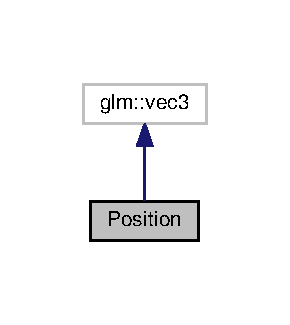
\includegraphics[width=139pt]{struct_position__inherit__graph}
\end{center}
\end{figure}


Collaboration diagram for Position\+:
\nopagebreak
\begin{figure}[H]
\begin{center}
\leavevmode
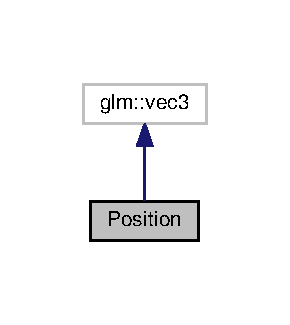
\includegraphics[width=139pt]{struct_position__coll__graph}
\end{center}
\end{figure}
\subsection*{Public Member Functions}
\begin{DoxyCompactItemize}
\item 
\hyperlink{struct_position_a369a577425f8ba02e8750d04b6a088db}{Position} ()
\item 
\hyperlink{struct_position_a75943ebda3e14f1b03a833745ccf9861}{Position} (float x, float y, float z)
\item 
glm\+::vec3 \hyperlink{struct_position_aaccc6084d199c1f5fd4a325df73caff8}{get\+Glm\+Vec3} ()
\item 
glm\+::vec4 \hyperlink{struct_position_a25a2270a1b1e0a97f0aa3a0ed37c5007}{get\+Glm\+Vec4} ()
\end{DoxyCompactItemize}


\subsection{Detailed Description}


Definition at line 8 of file Position.\+h.



\subsection{Constructor \& Destructor Documentation}
\mbox{\Hypertarget{struct_position_a369a577425f8ba02e8750d04b6a088db}\label{struct_position_a369a577425f8ba02e8750d04b6a088db}} 
\index{Position@{Position}!Position@{Position}}
\index{Position@{Position}!Position@{Position}}
\subsubsection{\texorpdfstring{Position()}{Position()}\hspace{0.1cm}{\footnotesize\ttfamily [1/2]}}
{\footnotesize\ttfamily Position\+::\+Position (\begin{DoxyParamCaption}{ }\end{DoxyParamCaption})\hspace{0.3cm}{\ttfamily [inline]}}



Definition at line 10 of file Position.\+h.

\mbox{\Hypertarget{struct_position_a75943ebda3e14f1b03a833745ccf9861}\label{struct_position_a75943ebda3e14f1b03a833745ccf9861}} 
\index{Position@{Position}!Position@{Position}}
\index{Position@{Position}!Position@{Position}}
\subsubsection{\texorpdfstring{Position()}{Position()}\hspace{0.1cm}{\footnotesize\ttfamily [2/2]}}
{\footnotesize\ttfamily Position\+::\+Position (\begin{DoxyParamCaption}\item[{float}]{x,  }\item[{float}]{y,  }\item[{float}]{z }\end{DoxyParamCaption})\hspace{0.3cm}{\ttfamily [inline]}}



Definition at line 11 of file Position.\+h.



\subsection{Member Function Documentation}
\mbox{\Hypertarget{struct_position_aaccc6084d199c1f5fd4a325df73caff8}\label{struct_position_aaccc6084d199c1f5fd4a325df73caff8}} 
\index{Position@{Position}!get\+Glm\+Vec3@{get\+Glm\+Vec3}}
\index{get\+Glm\+Vec3@{get\+Glm\+Vec3}!Position@{Position}}
\subsubsection{\texorpdfstring{get\+Glm\+Vec3()}{getGlmVec3()}}
{\footnotesize\ttfamily glm\+::vec3 Position\+::get\+Glm\+Vec3 (\begin{DoxyParamCaption}{ }\end{DoxyParamCaption})\hspace{0.3cm}{\ttfamily [inline]}}



Definition at line 13 of file Position.\+h.

\mbox{\Hypertarget{struct_position_a25a2270a1b1e0a97f0aa3a0ed37c5007}\label{struct_position_a25a2270a1b1e0a97f0aa3a0ed37c5007}} 
\index{Position@{Position}!get\+Glm\+Vec4@{get\+Glm\+Vec4}}
\index{get\+Glm\+Vec4@{get\+Glm\+Vec4}!Position@{Position}}
\subsubsection{\texorpdfstring{get\+Glm\+Vec4()}{getGlmVec4()}}
{\footnotesize\ttfamily glm\+::vec4 Position\+::get\+Glm\+Vec4 (\begin{DoxyParamCaption}{ }\end{DoxyParamCaption})\hspace{0.3cm}{\ttfamily [inline]}}



Definition at line 18 of file Position.\+h.



The documentation for this struct was generated from the following file\+:\begin{DoxyCompactItemize}
\item 
/home/rory/\+Projects/ece-\/6122-\/final-\/project/src/objects/\hyperlink{_position_8h}{Position.\+h}\end{DoxyCompactItemize}

\hypertarget{struct_program_config}{}\section{Program\+Config Struct Reference}
\label{struct_program_config}\index{Program\+Config@{Program\+Config}}


{\ttfamily \#include $<$Program\+Config.\+h$>$}

\subsection*{Public Member Functions}
\begin{DoxyCompactItemize}
\item 
\hyperlink{struct_program_config_ac2d47c453cf5f99370097f9aa8c75ded}{Program\+Config} ()
\end{DoxyCompactItemize}
\subsection*{Public Attributes}
\begin{DoxyCompactItemize}
\item 
char \hyperlink{struct_program_config_a6673c608d617371fda38de237c9cab1e}{output\+\_\+filename} \mbox{[}128\mbox{]}
\item 
int \hyperlink{struct_program_config_a2e5a432549c56826d91022c2acd4ad71}{raytrace}
\item 
int \hyperlink{struct_program_config_ad3a77eb9d22a5ab56326a798cc8428d2}{num\+Threads}
\item 
int \hyperlink{struct_program_config_a19e30fc75258bd6a0d571432cb8c28ed}{stop\+Time\+\_\+s}
\item 
int \hyperlink{struct_program_config_ad059c9912c59ac0e8271114a4bb87c98}{verbose}
\end{DoxyCompactItemize}


\subsection{Detailed Description}
This is a structure to holds all the various program configuration options. This is passed around to the various modules of the code 

Definition at line 13 of file Program\+Config.\+h.



\subsection{Constructor \& Destructor Documentation}
\mbox{\Hypertarget{struct_program_config_ac2d47c453cf5f99370097f9aa8c75ded}\label{struct_program_config_ac2d47c453cf5f99370097f9aa8c75ded}} 
\index{Program\+Config@{Program\+Config}!Program\+Config@{Program\+Config}}
\index{Program\+Config@{Program\+Config}!Program\+Config@{Program\+Config}}
\subsubsection{\texorpdfstring{Program\+Config()}{ProgramConfig()}}
{\footnotesize\ttfamily Program\+Config\+::\+Program\+Config (\begin{DoxyParamCaption}{ }\end{DoxyParamCaption})\hspace{0.3cm}{\ttfamily [inline]}}



Definition at line 15 of file Program\+Config.\+h.



\subsection{Member Data Documentation}
\mbox{\Hypertarget{struct_program_config_ad3a77eb9d22a5ab56326a798cc8428d2}\label{struct_program_config_ad3a77eb9d22a5ab56326a798cc8428d2}} 
\index{Program\+Config@{Program\+Config}!num\+Threads@{num\+Threads}}
\index{num\+Threads@{num\+Threads}!Program\+Config@{Program\+Config}}
\subsubsection{\texorpdfstring{num\+Threads}{numThreads}}
{\footnotesize\ttfamily int Program\+Config\+::num\+Threads}



Definition at line 27 of file Program\+Config.\+h.

\mbox{\Hypertarget{struct_program_config_a6673c608d617371fda38de237c9cab1e}\label{struct_program_config_a6673c608d617371fda38de237c9cab1e}} 
\index{Program\+Config@{Program\+Config}!output\+\_\+filename@{output\+\_\+filename}}
\index{output\+\_\+filename@{output\+\_\+filename}!Program\+Config@{Program\+Config}}
\subsubsection{\texorpdfstring{output\+\_\+filename}{output\_filename}}
{\footnotesize\ttfamily char Program\+Config\+::output\+\_\+filename\mbox{[}128\mbox{]}}



Definition at line 25 of file Program\+Config.\+h.

\mbox{\Hypertarget{struct_program_config_a2e5a432549c56826d91022c2acd4ad71}\label{struct_program_config_a2e5a432549c56826d91022c2acd4ad71}} 
\index{Program\+Config@{Program\+Config}!raytrace@{raytrace}}
\index{raytrace@{raytrace}!Program\+Config@{Program\+Config}}
\subsubsection{\texorpdfstring{raytrace}{raytrace}}
{\footnotesize\ttfamily int Program\+Config\+::raytrace}



Definition at line 26 of file Program\+Config.\+h.

\mbox{\Hypertarget{struct_program_config_a19e30fc75258bd6a0d571432cb8c28ed}\label{struct_program_config_a19e30fc75258bd6a0d571432cb8c28ed}} 
\index{Program\+Config@{Program\+Config}!stop\+Time\+\_\+s@{stop\+Time\+\_\+s}}
\index{stop\+Time\+\_\+s@{stop\+Time\+\_\+s}!Program\+Config@{Program\+Config}}
\subsubsection{\texorpdfstring{stop\+Time\+\_\+s}{stopTime\_s}}
{\footnotesize\ttfamily int Program\+Config\+::stop\+Time\+\_\+s}



Definition at line 28 of file Program\+Config.\+h.

\mbox{\Hypertarget{struct_program_config_ad059c9912c59ac0e8271114a4bb87c98}\label{struct_program_config_ad059c9912c59ac0e8271114a4bb87c98}} 
\index{Program\+Config@{Program\+Config}!verbose@{verbose}}
\index{verbose@{verbose}!Program\+Config@{Program\+Config}}
\subsubsection{\texorpdfstring{verbose}{verbose}}
{\footnotesize\ttfamily int Program\+Config\+::verbose}



Definition at line 29 of file Program\+Config.\+h.



The documentation for this struct was generated from the following file\+:\begin{DoxyCompactItemize}
\item 
/home/rory/\+Projects/ece-\/6122-\/final-\/project/src/\hyperlink{_program_config_8h}{Program\+Config.\+h}\end{DoxyCompactItemize}

\hypertarget{class_raytracer}{}\section{Raytracer Class Reference}
\label{class_raytracer}\index{Raytracer@{Raytracer}}


{\ttfamily \#include $<$Raytracer.\+h$>$}

\subsection*{Public Member Functions}
\begin{DoxyCompactItemize}
\item 
\hyperlink{class_raytracer_a6be8b2ac76c00c1a59f507ebb51a94f9}{Raytracer} (unsigned int width, unsigned int height, float fov)
\item 
\hyperlink{class_raytracer_a610ba0d74edf864c8ed78c5d85c4480a}{$\sim$\+Raytracer} ()
\item 
void \hyperlink{class_raytracer_a881ef245d223dd1c9654b6f41c3e0a10}{render} (const std\+::vector$<$ \hyperlink{class_object}{Object} $\ast$$>$ \&objects)
\end{DoxyCompactItemize}


\subsection{Detailed Description}


Definition at line 10 of file Raytracer.\+h.



\subsection{Constructor \& Destructor Documentation}
\mbox{\Hypertarget{class_raytracer_a6be8b2ac76c00c1a59f507ebb51a94f9}\label{class_raytracer_a6be8b2ac76c00c1a59f507ebb51a94f9}} 
\index{Raytracer@{Raytracer}!Raytracer@{Raytracer}}
\index{Raytracer@{Raytracer}!Raytracer@{Raytracer}}
\subsubsection{\texorpdfstring{Raytracer()}{Raytracer()}}
{\footnotesize\ttfamily Raytracer\+::\+Raytracer (\begin{DoxyParamCaption}\item[{unsigned int}]{width,  }\item[{unsigned int}]{height,  }\item[{float}]{fov }\end{DoxyParamCaption})}

Constructor 
\begin{DoxyParams}{Parameters}
{\em width} & T\+O\+DO Document \\
\hline
{\em height} & T\+O\+DO Document \\
\hline
{\em fov} & T\+O\+DO Document \\
\hline
\end{DoxyParams}


Definition at line 157 of file Raytracer.\+cpp.

\mbox{\Hypertarget{class_raytracer_a610ba0d74edf864c8ed78c5d85c4480a}\label{class_raytracer_a610ba0d74edf864c8ed78c5d85c4480a}} 
\index{Raytracer@{Raytracer}!````~Raytracer@{$\sim$\+Raytracer}}
\index{````~Raytracer@{$\sim$\+Raytracer}!Raytracer@{Raytracer}}
\subsubsection{\texorpdfstring{$\sim$\+Raytracer()}{~Raytracer()}}
{\footnotesize\ttfamily Raytracer\+::$\sim$\+Raytracer (\begin{DoxyParamCaption}{ }\end{DoxyParamCaption})}

Destructor 

Definition at line 173 of file Raytracer.\+cpp.



\subsection{Member Function Documentation}
\mbox{\Hypertarget{class_raytracer_a881ef245d223dd1c9654b6f41c3e0a10}\label{class_raytracer_a881ef245d223dd1c9654b6f41c3e0a10}} 
\index{Raytracer@{Raytracer}!render@{render}}
\index{render@{render}!Raytracer@{Raytracer}}
\subsubsection{\texorpdfstring{render()}{render()}}
{\footnotesize\ttfamily void Raytracer\+::render (\begin{DoxyParamCaption}\item[{const std\+::vector$<$ \hyperlink{class_object}{Object} $\ast$$>$ \&}]{objects }\end{DoxyParamCaption})}

This is the rendering function. A camera ray for each pixel of the image is computed and then traced and finally returned with a color. If the ray hits a sphere, the color of the sphere at the intersection point is returned, else we return the background color. 
\begin{DoxyParams}{Parameters}
{\em spheres} & T\+O\+DO Document \\
\hline
\end{DoxyParams}


Definition at line 185 of file Raytracer.\+cpp.



The documentation for this class was generated from the following files\+:\begin{DoxyCompactItemize}
\item 
/home/rory/\+Projects/ece-\/6122-\/final-\/project/src/raytracer/\hyperlink{_raytracer_8h}{Raytracer.\+h}\item 
/home/rory/\+Projects/ece-\/6122-\/final-\/project/src/raytracer/\hyperlink{_raytracer_8cpp}{Raytracer.\+cpp}\end{DoxyCompactItemize}

\hypertarget{class_renderer}{}\section{Renderer Class Reference}
\label{class_renderer}\index{Renderer@{Renderer}}


{\ttfamily \#include $<$Renderer.\+h$>$}

\subsection*{Public Member Functions}
\begin{DoxyCompactItemize}
\item 
\hyperlink{class_renderer_ab00d964ee94277771d706281d58dc5d6}{Renderer} (\hyperlink{class_shader}{Shader} $\ast$shader)
\item 
\hyperlink{class_renderer_afeee408862d5bd6255a6882d47e6d5cd}{$\sim$\+Renderer} ()
\item 
void \hyperlink{class_renderer_a51ce7e0195b0f751ad65a5f1fe0ad0c4}{submit} (const \hyperlink{class_object}{Object} $\ast$object)
\item 
void \hyperlink{class_renderer_a18316a088e902f0f737c345c860e997d}{flush} (const glm\+::vec3 \&eye\+Position)
\end{DoxyCompactItemize}


\subsection{Detailed Description}


Definition at line 24 of file Renderer.\+h.



\subsection{Constructor \& Destructor Documentation}
\mbox{\Hypertarget{class_renderer_ab00d964ee94277771d706281d58dc5d6}\label{class_renderer_ab00d964ee94277771d706281d58dc5d6}} 
\index{Renderer@{Renderer}!Renderer@{Renderer}}
\index{Renderer@{Renderer}!Renderer@{Renderer}}
\subsubsection{\texorpdfstring{Renderer()}{Renderer()}}
{\footnotesize\ttfamily Renderer\+::\+Renderer (\begin{DoxyParamCaption}\item[{\hyperlink{class_shader}{Shader} $\ast$}]{shader }\end{DoxyParamCaption})}

Constructor 

Definition at line 8 of file Renderer.\+cpp.

\mbox{\Hypertarget{class_renderer_afeee408862d5bd6255a6882d47e6d5cd}\label{class_renderer_afeee408862d5bd6255a6882d47e6d5cd}} 
\index{Renderer@{Renderer}!````~Renderer@{$\sim$\+Renderer}}
\index{````~Renderer@{$\sim$\+Renderer}!Renderer@{Renderer}}
\subsubsection{\texorpdfstring{$\sim$\+Renderer()}{~Renderer()}}
{\footnotesize\ttfamily Renderer\+::$\sim$\+Renderer (\begin{DoxyParamCaption}{ }\end{DoxyParamCaption})}

Destructor 

Definition at line 77 of file Renderer.\+cpp.



\subsection{Member Function Documentation}
\mbox{\Hypertarget{class_renderer_a18316a088e902f0f737c345c860e997d}\label{class_renderer_a18316a088e902f0f737c345c860e997d}} 
\index{Renderer@{Renderer}!flush@{flush}}
\index{flush@{flush}!Renderer@{Renderer}}
\subsubsection{\texorpdfstring{flush()}{flush()}}
{\footnotesize\ttfamily void Renderer\+::flush (\begin{DoxyParamCaption}\item[{const glm\+::vec3 \&}]{eye\+Position }\end{DoxyParamCaption})}

Draws the triangles in this batch to the back buffer 

Definition at line 223 of file Renderer.\+cpp.

\mbox{\Hypertarget{class_renderer_a51ce7e0195b0f751ad65a5f1fe0ad0c4}\label{class_renderer_a51ce7e0195b0f751ad65a5f1fe0ad0c4}} 
\index{Renderer@{Renderer}!submit@{submit}}
\index{submit@{submit}!Renderer@{Renderer}}
\subsubsection{\texorpdfstring{submit()}{submit()}}
{\footnotesize\ttfamily void Renderer\+::submit (\begin{DoxyParamCaption}\item[{const \hyperlink{class_object}{Object} $\ast$}]{object }\end{DoxyParamCaption})}

T\+O\+DO 
\begin{DoxyParams}{Parameters}
{\em object} & T\+O\+DO \\
\hline
\end{DoxyParams}


Definition at line 88 of file Renderer.\+cpp.



The documentation for this class was generated from the following files\+:\begin{DoxyCompactItemize}
\item 
/home/rory/\+Projects/ece-\/6122-\/final-\/project/src/\hyperlink{_renderer_8h}{Renderer.\+h}\item 
/home/rory/\+Projects/ece-\/6122-\/final-\/project/src/\hyperlink{_renderer_8cpp}{Renderer.\+cpp}\end{DoxyCompactItemize}

\hypertarget{class_shader}{}\section{Shader Class Reference}
\label{class_shader}\index{Shader@{Shader}}


{\ttfamily \#include $<$Shader.\+h$>$}

\subsection*{Public Member Functions}
\begin{DoxyCompactItemize}
\item 
\hyperlink{class_shader_ae2a0af7abf90c72ab25a394a24ea92f1}{Shader} (const char $\ast$vert\+\_\+path, const char $\ast$frag\+\_\+path)
\item 
\hyperlink{class_shader_aff01df87e8a102f270b5b135a295e59d}{$\sim$\+Shader} ()
\item 
void \hyperlink{class_shader_a048e3e3d86daff7b8f61432a866c529f}{enable} () const
\item 
void \hyperlink{class_shader_af962c95adc950bd28afbc81631ad3957}{disable} () const
\item 
G\+Luint \hyperlink{class_shader_a3e18d47a57e86322c1e76bf78f13ca17}{get\+\_\+id} () const
\item 
G\+Lint \hyperlink{class_shader_a6dda73168720b8d4871f9a2340c914d0}{get\+Attrib\+Location} (const char $\ast$name)
\item 
void \hyperlink{class_shader_aee904a5bc799d32e28a9007f82f7c8f3}{enable\+Vertex\+Attrib\+Array} (const G\+Lchar $\ast$name)
\item 
void \hyperlink{class_shader_a7f5da760f0edbd72487f8d7905cf4216}{disable\+Vertex\+Attrib\+Array} (const G\+Lchar $\ast$name)
\item 
void \hyperlink{class_shader_af496d61361a0bde57ccb34e2d5933c43}{set\+Uniform1f} (const G\+Lchar $\ast$name, const float val)
\item 
void \hyperlink{class_shader_a9e34828e84023305a0a9454b20ebae8e}{set\+Uniform1i} (const G\+Lchar $\ast$name, const int val)
\item 
void \hyperlink{class_shader_a80c178459f4ac07e83c53a95dc1c5ec8}{set\+Uniform2f} (const G\+Lchar $\ast$name, const glm\+::vec2 \&val)
\item 
void \hyperlink{class_shader_a3ea68dd9c68a88fcc2d7abe873c9ecf2}{set\+Uniform3f} (const G\+Lchar $\ast$name, const glm\+::vec3 \&val)
\item 
void \hyperlink{class_shader_a3ae217faa57e267bfd54fe91cd72b6ba}{set\+Uniform4f} (const G\+Lchar $\ast$name, const glm\+::vec4 \&val)
\item 
void \hyperlink{class_shader_a15647c94eb01764b51527eb00f85c9c3}{set\+Uniform4fv} (const G\+Lchar $\ast$name, G\+Lsizei count, const G\+Lfloat $\ast$val)
\item 
void \hyperlink{class_shader_a15a1246f61f63dd1d202bb59447dc191}{set\+Uniform\+Mat4} (const G\+Lchar $\ast$name, const glm\+::mat4 \&val)
\end{DoxyCompactItemize}


\subsection{Detailed Description}


Definition at line 8 of file Shader.\+h.



\subsection{Constructor \& Destructor Documentation}
\mbox{\Hypertarget{class_shader_ae2a0af7abf90c72ab25a394a24ea92f1}\label{class_shader_ae2a0af7abf90c72ab25a394a24ea92f1}} 
\index{Shader@{Shader}!Shader@{Shader}}
\index{Shader@{Shader}!Shader@{Shader}}
\subsubsection{\texorpdfstring{Shader()}{Shader()}}
{\footnotesize\ttfamily Shader\+::\+Shader (\begin{DoxyParamCaption}\item[{const char $\ast$}]{vert\+\_\+path,  }\item[{const char $\ast$}]{frag\+\_\+path }\end{DoxyParamCaption})}

Constructor 
\begin{DoxyParams}{Parameters}
{\em vert\+\_\+path} & File path to the vertex shader \\
\hline
{\em frag\+\_\+path} & File path to the fragment shader \\
\hline
\end{DoxyParams}


Definition at line 13 of file Shader.\+cpp.

\mbox{\Hypertarget{class_shader_aff01df87e8a102f270b5b135a295e59d}\label{class_shader_aff01df87e8a102f270b5b135a295e59d}} 
\index{Shader@{Shader}!````~Shader@{$\sim$\+Shader}}
\index{````~Shader@{$\sim$\+Shader}!Shader@{Shader}}
\subsubsection{\texorpdfstring{$\sim$\+Shader()}{~Shader()}}
{\footnotesize\ttfamily Shader\+::$\sim$\+Shader (\begin{DoxyParamCaption}{ }\end{DoxyParamCaption})}

Destructor 

Definition at line 22 of file Shader.\+cpp.



\subsection{Member Function Documentation}
\mbox{\Hypertarget{class_shader_af962c95adc950bd28afbc81631ad3957}\label{class_shader_af962c95adc950bd28afbc81631ad3957}} 
\index{Shader@{Shader}!disable@{disable}}
\index{disable@{disable}!Shader@{Shader}}
\subsubsection{\texorpdfstring{disable()}{disable()}}
{\footnotesize\ttfamily void Shader\+::disable (\begin{DoxyParamCaption}{ }\end{DoxyParamCaption}) const}

Disables use of the shader program 

Definition at line 38 of file Shader.\+cpp.

\mbox{\Hypertarget{class_shader_a7f5da760f0edbd72487f8d7905cf4216}\label{class_shader_a7f5da760f0edbd72487f8d7905cf4216}} 
\index{Shader@{Shader}!disable\+Vertex\+Attrib\+Array@{disable\+Vertex\+Attrib\+Array}}
\index{disable\+Vertex\+Attrib\+Array@{disable\+Vertex\+Attrib\+Array}!Shader@{Shader}}
\subsubsection{\texorpdfstring{disable\+Vertex\+Attrib\+Array()}{disableVertexAttribArray()}}
{\footnotesize\ttfamily void Shader\+::disable\+Vertex\+Attrib\+Array (\begin{DoxyParamCaption}\item[{const G\+Lchar $\ast$}]{name }\end{DoxyParamCaption})}

Enables a vertex attrib array 
\begin{DoxyParams}{Parameters}
{\em name} & Points to a null terminated string containing the name of the attribute variable to enable \\
\hline
\end{DoxyParams}


Definition at line 223 of file Shader.\+cpp.

\mbox{\Hypertarget{class_shader_a048e3e3d86daff7b8f61432a866c529f}\label{class_shader_a048e3e3d86daff7b8f61432a866c529f}} 
\index{Shader@{Shader}!enable@{enable}}
\index{enable@{enable}!Shader@{Shader}}
\subsubsection{\texorpdfstring{enable()}{enable()}}
{\footnotesize\ttfamily void Shader\+::enable (\begin{DoxyParamCaption}{ }\end{DoxyParamCaption}) const}

Enables use of the shader program 

Definition at line 30 of file Shader.\+cpp.

\mbox{\Hypertarget{class_shader_aee904a5bc799d32e28a9007f82f7c8f3}\label{class_shader_aee904a5bc799d32e28a9007f82f7c8f3}} 
\index{Shader@{Shader}!enable\+Vertex\+Attrib\+Array@{enable\+Vertex\+Attrib\+Array}}
\index{enable\+Vertex\+Attrib\+Array@{enable\+Vertex\+Attrib\+Array}!Shader@{Shader}}
\subsubsection{\texorpdfstring{enable\+Vertex\+Attrib\+Array()}{enableVertexAttribArray()}}
{\footnotesize\ttfamily void Shader\+::enable\+Vertex\+Attrib\+Array (\begin{DoxyParamCaption}\item[{const G\+Lchar $\ast$}]{name }\end{DoxyParamCaption})}

Enables a vertex attrib array 
\begin{DoxyParams}{Parameters}
{\em name} & Points to a null terminated string containing the name of the attribute variable to enable \\
\hline
\end{DoxyParams}


Definition at line 211 of file Shader.\+cpp.

\mbox{\Hypertarget{class_shader_a3e18d47a57e86322c1e76bf78f13ca17}\label{class_shader_a3e18d47a57e86322c1e76bf78f13ca17}} 
\index{Shader@{Shader}!get\+\_\+id@{get\+\_\+id}}
\index{get\+\_\+id@{get\+\_\+id}!Shader@{Shader}}
\subsubsection{\texorpdfstring{get\+\_\+id()}{get\_id()}}
{\footnotesize\ttfamily G\+Luint Shader\+::get\+\_\+id (\begin{DoxyParamCaption}{ }\end{DoxyParamCaption}) const\hspace{0.3cm}{\ttfamily [inline]}}



Definition at line 17 of file Shader.\+h.

\mbox{\Hypertarget{class_shader_a6dda73168720b8d4871f9a2340c914d0}\label{class_shader_a6dda73168720b8d4871f9a2340c914d0}} 
\index{Shader@{Shader}!get\+Attrib\+Location@{get\+Attrib\+Location}}
\index{get\+Attrib\+Location@{get\+Attrib\+Location}!Shader@{Shader}}
\subsubsection{\texorpdfstring{get\+Attrib\+Location()}{getAttribLocation()}}
{\footnotesize\ttfamily G\+Lint Shader\+::get\+Attrib\+Location (\begin{DoxyParamCaption}\item[{const char $\ast$}]{name }\end{DoxyParamCaption})}

Returns the location of an attribute variable 
\begin{DoxyParams}{Parameters}
{\em name} & Points to a null terminated string containing the name of the attribute variable whose location is to be queried \\
\hline
\end{DoxyParams}
\begin{DoxyReturn}{Returns}
Returns the location of the attribute variable on success, else -\/1 or error 
\end{DoxyReturn}


Definition at line 201 of file Shader.\+cpp.

\mbox{\Hypertarget{class_shader_af496d61361a0bde57ccb34e2d5933c43}\label{class_shader_af496d61361a0bde57ccb34e2d5933c43}} 
\index{Shader@{Shader}!set\+Uniform1f@{set\+Uniform1f}}
\index{set\+Uniform1f@{set\+Uniform1f}!Shader@{Shader}}
\subsubsection{\texorpdfstring{set\+Uniform1f()}{setUniform1f()}}
{\footnotesize\ttfamily void Shader\+::set\+Uniform1f (\begin{DoxyParamCaption}\item[{const G\+Lchar $\ast$}]{name,  }\item[{const float}]{val }\end{DoxyParamCaption})}

Specify the value of a uniform variable for the current program object 
\begin{DoxyParams}{Parameters}
{\em name} & T\+O\+DO \\
\hline
{\em val} & T\+O\+DO \\
\hline
\end{DoxyParams}


Definition at line 48 of file Shader.\+cpp.

\mbox{\Hypertarget{class_shader_a9e34828e84023305a0a9454b20ebae8e}\label{class_shader_a9e34828e84023305a0a9454b20ebae8e}} 
\index{Shader@{Shader}!set\+Uniform1i@{set\+Uniform1i}}
\index{set\+Uniform1i@{set\+Uniform1i}!Shader@{Shader}}
\subsubsection{\texorpdfstring{set\+Uniform1i()}{setUniform1i()}}
{\footnotesize\ttfamily void Shader\+::set\+Uniform1i (\begin{DoxyParamCaption}\item[{const G\+Lchar $\ast$}]{name,  }\item[{const int}]{val }\end{DoxyParamCaption})}

Specify the value of a uniform variable for the current program object 
\begin{DoxyParams}{Parameters}
{\em name} & T\+O\+DO \\
\hline
{\em val} & T\+O\+DO \\
\hline
\end{DoxyParams}


Definition at line 58 of file Shader.\+cpp.

\mbox{\Hypertarget{class_shader_a80c178459f4ac07e83c53a95dc1c5ec8}\label{class_shader_a80c178459f4ac07e83c53a95dc1c5ec8}} 
\index{Shader@{Shader}!set\+Uniform2f@{set\+Uniform2f}}
\index{set\+Uniform2f@{set\+Uniform2f}!Shader@{Shader}}
\subsubsection{\texorpdfstring{set\+Uniform2f()}{setUniform2f()}}
{\footnotesize\ttfamily void Shader\+::set\+Uniform2f (\begin{DoxyParamCaption}\item[{const G\+Lchar $\ast$}]{name,  }\item[{const glm\+::vec2 \&}]{val }\end{DoxyParamCaption})}

Specify the value of a uniform variable for the current program object 
\begin{DoxyParams}{Parameters}
{\em name} & T\+O\+DO \\
\hline
{\em val} & T\+O\+DO \\
\hline
\end{DoxyParams}


Definition at line 68 of file Shader.\+cpp.

\mbox{\Hypertarget{class_shader_a3ea68dd9c68a88fcc2d7abe873c9ecf2}\label{class_shader_a3ea68dd9c68a88fcc2d7abe873c9ecf2}} 
\index{Shader@{Shader}!set\+Uniform3f@{set\+Uniform3f}}
\index{set\+Uniform3f@{set\+Uniform3f}!Shader@{Shader}}
\subsubsection{\texorpdfstring{set\+Uniform3f()}{setUniform3f()}}
{\footnotesize\ttfamily void Shader\+::set\+Uniform3f (\begin{DoxyParamCaption}\item[{const G\+Lchar $\ast$}]{name,  }\item[{const glm\+::vec3 \&}]{val }\end{DoxyParamCaption})}

Specify the value of a uniform variable for the current program object 
\begin{DoxyParams}{Parameters}
{\em name} & T\+O\+DO \\
\hline
{\em val} & T\+O\+DO \\
\hline
\end{DoxyParams}


Definition at line 78 of file Shader.\+cpp.

\mbox{\Hypertarget{class_shader_a3ae217faa57e267bfd54fe91cd72b6ba}\label{class_shader_a3ae217faa57e267bfd54fe91cd72b6ba}} 
\index{Shader@{Shader}!set\+Uniform4f@{set\+Uniform4f}}
\index{set\+Uniform4f@{set\+Uniform4f}!Shader@{Shader}}
\subsubsection{\texorpdfstring{set\+Uniform4f()}{setUniform4f()}}
{\footnotesize\ttfamily void Shader\+::set\+Uniform4f (\begin{DoxyParamCaption}\item[{const G\+Lchar $\ast$}]{name,  }\item[{const glm\+::vec4 \&}]{val }\end{DoxyParamCaption})}

Specify the value of a uniform variable for the current program object 
\begin{DoxyParams}{Parameters}
{\em name} & T\+O\+DO \\
\hline
{\em val} & T\+O\+DO \\
\hline
\end{DoxyParams}


Definition at line 88 of file Shader.\+cpp.

\mbox{\Hypertarget{class_shader_a15647c94eb01764b51527eb00f85c9c3}\label{class_shader_a15647c94eb01764b51527eb00f85c9c3}} 
\index{Shader@{Shader}!set\+Uniform4fv@{set\+Uniform4fv}}
\index{set\+Uniform4fv@{set\+Uniform4fv}!Shader@{Shader}}
\subsubsection{\texorpdfstring{set\+Uniform4fv()}{setUniform4fv()}}
{\footnotesize\ttfamily void Shader\+::set\+Uniform4fv (\begin{DoxyParamCaption}\item[{const G\+Lchar $\ast$}]{name,  }\item[{G\+Lsizei}]{count,  }\item[{const G\+Lfloat $\ast$}]{val }\end{DoxyParamCaption})}

Specify the value of a uniform variable for the current program object 
\begin{DoxyParams}{Parameters}
{\em name} & T\+O\+DO \\
\hline
{\em val} & T\+O\+DO \\
\hline
\end{DoxyParams}


Definition at line 102 of file Shader.\+cpp.

\mbox{\Hypertarget{class_shader_a15a1246f61f63dd1d202bb59447dc191}\label{class_shader_a15a1246f61f63dd1d202bb59447dc191}} 
\index{Shader@{Shader}!set\+Uniform\+Mat4@{set\+Uniform\+Mat4}}
\index{set\+Uniform\+Mat4@{set\+Uniform\+Mat4}!Shader@{Shader}}
\subsubsection{\texorpdfstring{set\+Uniform\+Mat4()}{setUniformMat4()}}
{\footnotesize\ttfamily void Shader\+::set\+Uniform\+Mat4 (\begin{DoxyParamCaption}\item[{const G\+Lchar $\ast$}]{name,  }\item[{const glm\+::mat4 \&}]{val }\end{DoxyParamCaption})}

Specify the value of a uniform variable for the current program object 
\begin{DoxyParams}{Parameters}
{\em name} & T\+O\+DO \\
\hline
{\em val} & T\+O\+DO \\
\hline
\end{DoxyParams}


Definition at line 112 of file Shader.\+cpp.



The documentation for this class was generated from the following files\+:\begin{DoxyCompactItemize}
\item 
/home/rory/\+Projects/ece-\/6122-\/final-\/project/src/\hyperlink{_shader_8h}{Shader.\+h}\item 
/home/rory/\+Projects/ece-\/6122-\/final-\/project/src/\hyperlink{_shader_8cpp}{Shader.\+cpp}\end{DoxyCompactItemize}

\hypertarget{class_sphere}{}\section{Sphere Class Reference}
\label{class_sphere}\index{Sphere@{Sphere}}


{\ttfamily \#include $<$Sphere.\+h$>$}



Collaboration diagram for Sphere\+:
\nopagebreak
\begin{figure}[H]
\begin{center}
\leavevmode
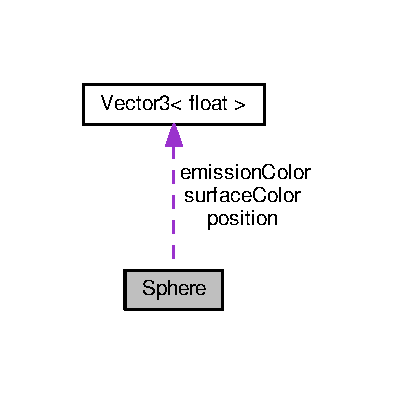
\includegraphics[width=190pt]{class_sphere__coll__graph}
\end{center}
\end{figure}
\subsection*{Public Member Functions}
\begin{DoxyCompactItemize}
\item 
\hyperlink{class_sphere_a46b4e530fe3204b5dfc0547cec96dbaa}{Sphere} (const \hyperlink{_vector3_8h_af345ad77ba5e240c7ab72b4b2077e754}{Vector3f} \&c, const float \&r, const \hyperlink{_vector3_8h_af345ad77ba5e240c7ab72b4b2077e754}{Vector3f} \&sc, const float \&refl=0, const float \&transp=0, const \hyperlink{_vector3_8h_af345ad77ba5e240c7ab72b4b2077e754}{Vector3f} \&ec=0)
\item 
bool \hyperlink{class_sphere_a35ba0414bedd68d86349273db13cca7d}{intersect} (const \hyperlink{_vector3_8h_af345ad77ba5e240c7ab72b4b2077e754}{Vector3f} \&ray\+Origin, const \hyperlink{_vector3_8h_af345ad77ba5e240c7ab72b4b2077e754}{Vector3f} \&ray\+Direction, float \&t0, float \&t1) const
\end{DoxyCompactItemize}
\subsection*{Public Attributes}
\begin{DoxyCompactItemize}
\item 
\hyperlink{_vector3_8h_af345ad77ba5e240c7ab72b4b2077e754}{Vector3f} \hyperlink{class_sphere_a0458c2e8cd2b6472e6b32b4304b353d6}{position}
\item 
float \hyperlink{class_sphere_ae6f42f0da6679a2f0b4a22681ccccf38}{radius}
\item 
float \hyperlink{class_sphere_a676be49a940d037ac298e7010f03d416}{radius2}
\item 
\hyperlink{_vector3_8h_af345ad77ba5e240c7ab72b4b2077e754}{Vector3f} \hyperlink{class_sphere_accdb6ecbf2c62a19c495debfe7c3685a}{surface\+Color}
\item 
\hyperlink{_vector3_8h_af345ad77ba5e240c7ab72b4b2077e754}{Vector3f} \hyperlink{class_sphere_ab3bc31c7c6cd80578e755c85eb6e5894}{emission\+Color}
\item 
float \hyperlink{class_sphere_a93f7757b497ba9f0f93b9927e5d96e5d}{transparency}
\item 
float \hyperlink{class_sphere_a7b8835ace79e36f2cacf9ff0cb962fae}{reflection}
\end{DoxyCompactItemize}


\subsection{Detailed Description}


Definition at line 12 of file Sphere.\+h.



\subsection{Constructor \& Destructor Documentation}
\mbox{\Hypertarget{class_sphere_a46b4e530fe3204b5dfc0547cec96dbaa}\label{class_sphere_a46b4e530fe3204b5dfc0547cec96dbaa}} 
\index{Sphere@{Sphere}!Sphere@{Sphere}}
\index{Sphere@{Sphere}!Sphere@{Sphere}}
\subsubsection{\texorpdfstring{Sphere()}{Sphere()}}
{\footnotesize\ttfamily Sphere\+::\+Sphere (\begin{DoxyParamCaption}\item[{const \hyperlink{_vector3_8h_af345ad77ba5e240c7ab72b4b2077e754}{Vector3f} \&}]{c,  }\item[{const float \&}]{r,  }\item[{const \hyperlink{_vector3_8h_af345ad77ba5e240c7ab72b4b2077e754}{Vector3f} \&}]{sc,  }\item[{const float \&}]{refl = {\ttfamily 0},  }\item[{const float \&}]{transp = {\ttfamily 0},  }\item[{const \hyperlink{_vector3_8h_af345ad77ba5e240c7ab72b4b2077e754}{Vector3f} \&}]{ec = {\ttfamily 0} }\end{DoxyParamCaption})\hspace{0.3cm}{\ttfamily [inline]}}



Definition at line 22 of file Sphere.\+h.



\subsection{Member Function Documentation}
\mbox{\Hypertarget{class_sphere_a35ba0414bedd68d86349273db13cca7d}\label{class_sphere_a35ba0414bedd68d86349273db13cca7d}} 
\index{Sphere@{Sphere}!intersect@{intersect}}
\index{intersect@{intersect}!Sphere@{Sphere}}
\subsubsection{\texorpdfstring{intersect()}{intersect()}}
{\footnotesize\ttfamily bool Sphere\+::intersect (\begin{DoxyParamCaption}\item[{const \hyperlink{_vector3_8h_af345ad77ba5e240c7ab72b4b2077e754}{Vector3f} \&}]{ray\+Origin,  }\item[{const \hyperlink{_vector3_8h_af345ad77ba5e240c7ab72b4b2077e754}{Vector3f} \&}]{ray\+Direction,  }\item[{float \&}]{t0,  }\item[{float \&}]{t1 }\end{DoxyParamCaption}) const\hspace{0.3cm}{\ttfamily [inline]}}



Definition at line 33 of file Sphere.\+h.



\subsection{Member Data Documentation}
\mbox{\Hypertarget{class_sphere_ab3bc31c7c6cd80578e755c85eb6e5894}\label{class_sphere_ab3bc31c7c6cd80578e755c85eb6e5894}} 
\index{Sphere@{Sphere}!emission\+Color@{emission\+Color}}
\index{emission\+Color@{emission\+Color}!Sphere@{Sphere}}
\subsubsection{\texorpdfstring{emission\+Color}{emissionColor}}
{\footnotesize\ttfamily \hyperlink{_vector3_8h_af345ad77ba5e240c7ab72b4b2077e754}{Vector3f} Sphere\+::emission\+Color}



Definition at line 18 of file Sphere.\+h.

\mbox{\Hypertarget{class_sphere_a0458c2e8cd2b6472e6b32b4304b353d6}\label{class_sphere_a0458c2e8cd2b6472e6b32b4304b353d6}} 
\index{Sphere@{Sphere}!position@{position}}
\index{position@{position}!Sphere@{Sphere}}
\subsubsection{\texorpdfstring{position}{position}}
{\footnotesize\ttfamily \hyperlink{_vector3_8h_af345ad77ba5e240c7ab72b4b2077e754}{Vector3f} Sphere\+::position}



Definition at line 16 of file Sphere.\+h.

\mbox{\Hypertarget{class_sphere_ae6f42f0da6679a2f0b4a22681ccccf38}\label{class_sphere_ae6f42f0da6679a2f0b4a22681ccccf38}} 
\index{Sphere@{Sphere}!radius@{radius}}
\index{radius@{radius}!Sphere@{Sphere}}
\subsubsection{\texorpdfstring{radius}{radius}}
{\footnotesize\ttfamily float Sphere\+::radius}



Definition at line 17 of file Sphere.\+h.

\mbox{\Hypertarget{class_sphere_a676be49a940d037ac298e7010f03d416}\label{class_sphere_a676be49a940d037ac298e7010f03d416}} 
\index{Sphere@{Sphere}!radius2@{radius2}}
\index{radius2@{radius2}!Sphere@{Sphere}}
\subsubsection{\texorpdfstring{radius2}{radius2}}
{\footnotesize\ttfamily float Sphere\+::radius2}



Definition at line 17 of file Sphere.\+h.

\mbox{\Hypertarget{class_sphere_a7b8835ace79e36f2cacf9ff0cb962fae}\label{class_sphere_a7b8835ace79e36f2cacf9ff0cb962fae}} 
\index{Sphere@{Sphere}!reflection@{reflection}}
\index{reflection@{reflection}!Sphere@{Sphere}}
\subsubsection{\texorpdfstring{reflection}{reflection}}
{\footnotesize\ttfamily float Sphere\+::reflection}



Definition at line 19 of file Sphere.\+h.

\mbox{\Hypertarget{class_sphere_accdb6ecbf2c62a19c495debfe7c3685a}\label{class_sphere_accdb6ecbf2c62a19c495debfe7c3685a}} 
\index{Sphere@{Sphere}!surface\+Color@{surface\+Color}}
\index{surface\+Color@{surface\+Color}!Sphere@{Sphere}}
\subsubsection{\texorpdfstring{surface\+Color}{surfaceColor}}
{\footnotesize\ttfamily \hyperlink{_vector3_8h_af345ad77ba5e240c7ab72b4b2077e754}{Vector3f} Sphere\+::surface\+Color}



Definition at line 18 of file Sphere.\+h.

\mbox{\Hypertarget{class_sphere_a93f7757b497ba9f0f93b9927e5d96e5d}\label{class_sphere_a93f7757b497ba9f0f93b9927e5d96e5d}} 
\index{Sphere@{Sphere}!transparency@{transparency}}
\index{transparency@{transparency}!Sphere@{Sphere}}
\subsubsection{\texorpdfstring{transparency}{transparency}}
{\footnotesize\ttfamily float Sphere\+::transparency}



Definition at line 19 of file Sphere.\+h.



The documentation for this class was generated from the following file\+:\begin{DoxyCompactItemize}
\item 
/home/rory/\+Projects/ece-\/6122-\/final-\/project/src/raytracer/\hyperlink{_sphere_8h}{Sphere.\+h}\end{DoxyCompactItemize}

\hypertarget{struct_tex_coord}{}\section{Tex\+Coord Struct Reference}
\label{struct_tex_coord}\index{Tex\+Coord@{Tex\+Coord}}


{\ttfamily \#include $<$Tex\+Coord.\+h$>$}



Inheritance diagram for Tex\+Coord\+:
\nopagebreak
\begin{figure}[H]
\begin{center}
\leavevmode
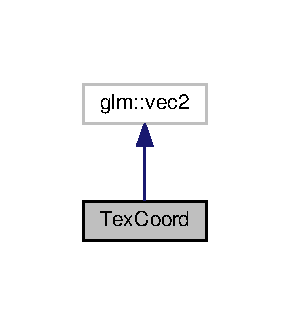
\includegraphics[width=139pt]{struct_tex_coord__inherit__graph}
\end{center}
\end{figure}


Collaboration diagram for Tex\+Coord\+:
\nopagebreak
\begin{figure}[H]
\begin{center}
\leavevmode
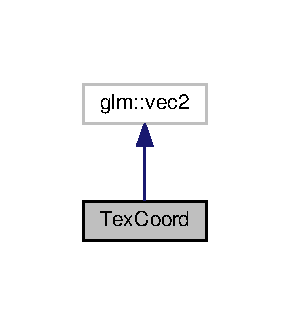
\includegraphics[width=139pt]{struct_tex_coord__coll__graph}
\end{center}
\end{figure}
\subsection*{Public Member Functions}
\begin{DoxyCompactItemize}
\item 
\hyperlink{struct_tex_coord_ae1167f68dab931cc523e1f74fa5ad206}{Tex\+Coord} ()
\item 
\hyperlink{struct_tex_coord_a02018ed90402d77cb313b581c0ea0561}{Tex\+Coord} (float x, float y)
\end{DoxyCompactItemize}


\subsection{Detailed Description}


Definition at line 8 of file Tex\+Coord.\+h.



\subsection{Constructor \& Destructor Documentation}
\mbox{\Hypertarget{struct_tex_coord_ae1167f68dab931cc523e1f74fa5ad206}\label{struct_tex_coord_ae1167f68dab931cc523e1f74fa5ad206}} 
\index{Tex\+Coord@{Tex\+Coord}!Tex\+Coord@{Tex\+Coord}}
\index{Tex\+Coord@{Tex\+Coord}!Tex\+Coord@{Tex\+Coord}}
\subsubsection{\texorpdfstring{Tex\+Coord()}{TexCoord()}\hspace{0.1cm}{\footnotesize\ttfamily [1/2]}}
{\footnotesize\ttfamily Tex\+Coord\+::\+Tex\+Coord (\begin{DoxyParamCaption}{ }\end{DoxyParamCaption})\hspace{0.3cm}{\ttfamily [inline]}}



Definition at line 10 of file Tex\+Coord.\+h.

\mbox{\Hypertarget{struct_tex_coord_a02018ed90402d77cb313b581c0ea0561}\label{struct_tex_coord_a02018ed90402d77cb313b581c0ea0561}} 
\index{Tex\+Coord@{Tex\+Coord}!Tex\+Coord@{Tex\+Coord}}
\index{Tex\+Coord@{Tex\+Coord}!Tex\+Coord@{Tex\+Coord}}
\subsubsection{\texorpdfstring{Tex\+Coord()}{TexCoord()}\hspace{0.1cm}{\footnotesize\ttfamily [2/2]}}
{\footnotesize\ttfamily Tex\+Coord\+::\+Tex\+Coord (\begin{DoxyParamCaption}\item[{float}]{x,  }\item[{float}]{y }\end{DoxyParamCaption})\hspace{0.3cm}{\ttfamily [inline]}}



Definition at line 11 of file Tex\+Coord.\+h.



The documentation for this struct was generated from the following file\+:\begin{DoxyCompactItemize}
\item 
/home/rory/\+Projects/ece-\/6122-\/final-\/project/src/objects/\hyperlink{_tex_coord_8h}{Tex\+Coord.\+h}\end{DoxyCompactItemize}

\hypertarget{class_texture}{}\section{Texture Class Reference}
\label{class_texture}\index{Texture@{Texture}}


{\ttfamily \#include $<$Texture.\+h$>$}

\subsection*{Public Member Functions}
\begin{DoxyCompactItemize}
\item 
\hyperlink{class_texture_ad5406229668e6ee741beddc3f37a38d1}{Texture} (const char $\ast$filepath)
\item 
\hyperlink{class_texture_a09c4bcb7462f64c1d20fa69dba3cee8a}{$\sim$\+Texture} ()
\item 
void \hyperlink{class_texture_a4b85391c6e54686ec566ba38c62dde98}{bind} () const
\item 
void \hyperlink{class_texture_a451d7afac3848417bb1007d39ee7d545}{unbind} () const
\item 
G\+Lsizei \hyperlink{class_texture_a29224e09dad7892ec84ea379703b512c}{get\+\_\+width} () const
\item 
G\+Lsizei \hyperlink{class_texture_afdc100805e42879c03439962c48f9dda}{get\+\_\+height} () const
\item 
G\+Luint \hyperlink{class_texture_a53aa350bde0fc93271c74e2bd2b391fa}{get\+\_\+id} () const
\end{DoxyCompactItemize}


\subsection{Detailed Description}


Definition at line 8 of file Texture.\+h.



\subsection{Constructor \& Destructor Documentation}
\mbox{\Hypertarget{class_texture_ad5406229668e6ee741beddc3f37a38d1}\label{class_texture_ad5406229668e6ee741beddc3f37a38d1}} 
\index{Texture@{Texture}!Texture@{Texture}}
\index{Texture@{Texture}!Texture@{Texture}}
\subsubsection{\texorpdfstring{Texture()}{Texture()}}
{\footnotesize\ttfamily Texture\+::\+Texture (\begin{DoxyParamCaption}\item[{const char $\ast$}]{filepath }\end{DoxyParamCaption})}



Definition at line 3 of file Texture.\+cpp.

\mbox{\Hypertarget{class_texture_a09c4bcb7462f64c1d20fa69dba3cee8a}\label{class_texture_a09c4bcb7462f64c1d20fa69dba3cee8a}} 
\index{Texture@{Texture}!````~Texture@{$\sim$\+Texture}}
\index{````~Texture@{$\sim$\+Texture}!Texture@{Texture}}
\subsubsection{\texorpdfstring{$\sim$\+Texture()}{~Texture()}}
{\footnotesize\ttfamily Texture\+::$\sim$\+Texture (\begin{DoxyParamCaption}{ }\end{DoxyParamCaption})}



Definition at line 30 of file Texture.\+cpp.



\subsection{Member Function Documentation}
\mbox{\Hypertarget{class_texture_a4b85391c6e54686ec566ba38c62dde98}\label{class_texture_a4b85391c6e54686ec566ba38c62dde98}} 
\index{Texture@{Texture}!bind@{bind}}
\index{bind@{bind}!Texture@{Texture}}
\subsubsection{\texorpdfstring{bind()}{bind()}}
{\footnotesize\ttfamily void Texture\+::bind (\begin{DoxyParamCaption}{ }\end{DoxyParamCaption}) const}



Definition at line 35 of file Texture.\+cpp.

\mbox{\Hypertarget{class_texture_afdc100805e42879c03439962c48f9dda}\label{class_texture_afdc100805e42879c03439962c48f9dda}} 
\index{Texture@{Texture}!get\+\_\+height@{get\+\_\+height}}
\index{get\+\_\+height@{get\+\_\+height}!Texture@{Texture}}
\subsubsection{\texorpdfstring{get\+\_\+height()}{get\_height()}}
{\footnotesize\ttfamily G\+Lsizei Texture\+::get\+\_\+height (\begin{DoxyParamCaption}{ }\end{DoxyParamCaption}) const\hspace{0.3cm}{\ttfamily [inline]}}



Definition at line 18 of file Texture.\+h.

\mbox{\Hypertarget{class_texture_a53aa350bde0fc93271c74e2bd2b391fa}\label{class_texture_a53aa350bde0fc93271c74e2bd2b391fa}} 
\index{Texture@{Texture}!get\+\_\+id@{get\+\_\+id}}
\index{get\+\_\+id@{get\+\_\+id}!Texture@{Texture}}
\subsubsection{\texorpdfstring{get\+\_\+id()}{get\_id()}}
{\footnotesize\ttfamily G\+Luint Texture\+::get\+\_\+id (\begin{DoxyParamCaption}{ }\end{DoxyParamCaption}) const\hspace{0.3cm}{\ttfamily [inline]}}



Definition at line 19 of file Texture.\+h.

\mbox{\Hypertarget{class_texture_a29224e09dad7892ec84ea379703b512c}\label{class_texture_a29224e09dad7892ec84ea379703b512c}} 
\index{Texture@{Texture}!get\+\_\+width@{get\+\_\+width}}
\index{get\+\_\+width@{get\+\_\+width}!Texture@{Texture}}
\subsubsection{\texorpdfstring{get\+\_\+width()}{get\_width()}}
{\footnotesize\ttfamily G\+Lsizei Texture\+::get\+\_\+width (\begin{DoxyParamCaption}{ }\end{DoxyParamCaption}) const\hspace{0.3cm}{\ttfamily [inline]}}



Definition at line 17 of file Texture.\+h.

\mbox{\Hypertarget{class_texture_a451d7afac3848417bb1007d39ee7d545}\label{class_texture_a451d7afac3848417bb1007d39ee7d545}} 
\index{Texture@{Texture}!unbind@{unbind}}
\index{unbind@{unbind}!Texture@{Texture}}
\subsubsection{\texorpdfstring{unbind()}{unbind()}}
{\footnotesize\ttfamily void Texture\+::unbind (\begin{DoxyParamCaption}{ }\end{DoxyParamCaption}) const}



Definition at line 40 of file Texture.\+cpp.



The documentation for this class was generated from the following files\+:\begin{DoxyCompactItemize}
\item 
/home/rory/\+Projects/ece-\/6122-\/final-\/project/src/objects/\hyperlink{_texture_8h}{Texture.\+h}\item 
/home/rory/\+Projects/ece-\/6122-\/final-\/project/src/objects/\hyperlink{_texture_8cpp}{Texture.\+cpp}\end{DoxyCompactItemize}

\hypertarget{class_text_writer}{}\section{Text\+Writer Class Reference}
\label{class_text_writer}\index{Text\+Writer@{Text\+Writer}}


{\ttfamily \#include $<$Text\+Writer.\+h$>$}

\subsection*{Public Member Functions}
\begin{DoxyCompactItemize}
\item 
\hyperlink{class_text_writer_aa1b80a78641197e5ec41a5a8b29f9101}{Text\+Writer} (const char $\ast$vertex\+\_\+path, const char $\ast$fragment\+\_\+path, const char $\ast$ttf\+\_\+path, int font\+\_\+size)
\item 
\hyperlink{class_text_writer_aab0c50e9ffcd9fe2797753b222ad1641}{$\sim$\+Text\+Writer} ()
\item 
void \hyperlink{class_text_writer_aa120043668d4eba84d41222c0dbd3b86}{begin} ()
\item 
void \hyperlink{class_text_writer_a725e9275d2826c823947e790611ad9ca}{end} ()
\item 
void \hyperlink{class_text_writer_a26b8bbd68df18171d18eafd7ebaab8e3}{write} (const char $\ast$text, float x, float y, float sx, float sy, const glm\+::vec4 \&color)
\end{DoxyCompactItemize}


\subsection{Detailed Description}


Definition at line 17 of file Text\+Writer.\+h.



\subsection{Constructor \& Destructor Documentation}
\mbox{\Hypertarget{class_text_writer_aa1b80a78641197e5ec41a5a8b29f9101}\label{class_text_writer_aa1b80a78641197e5ec41a5a8b29f9101}} 
\index{Text\+Writer@{Text\+Writer}!Text\+Writer@{Text\+Writer}}
\index{Text\+Writer@{Text\+Writer}!Text\+Writer@{Text\+Writer}}
\subsubsection{\texorpdfstring{Text\+Writer()}{TextWriter()}}
{\footnotesize\ttfamily Text\+Writer\+::\+Text\+Writer (\begin{DoxyParamCaption}\item[{const char $\ast$}]{vertex\+\_\+path,  }\item[{const char $\ast$}]{fragment\+\_\+path,  }\item[{const char $\ast$}]{ttf\+\_\+path,  }\item[{int}]{font\+\_\+size }\end{DoxyParamCaption})}



Definition at line 148 of file Text\+Writer.\+cpp.

\mbox{\Hypertarget{class_text_writer_aab0c50e9ffcd9fe2797753b222ad1641}\label{class_text_writer_aab0c50e9ffcd9fe2797753b222ad1641}} 
\index{Text\+Writer@{Text\+Writer}!````~Text\+Writer@{$\sim$\+Text\+Writer}}
\index{````~Text\+Writer@{$\sim$\+Text\+Writer}!Text\+Writer@{Text\+Writer}}
\subsubsection{\texorpdfstring{$\sim$\+Text\+Writer()}{~TextWriter()}}
{\footnotesize\ttfamily Text\+Writer\+::$\sim$\+Text\+Writer (\begin{DoxyParamCaption}{ }\end{DoxyParamCaption})}



Definition at line 167 of file Text\+Writer.\+cpp.



\subsection{Member Function Documentation}
\mbox{\Hypertarget{class_text_writer_aa120043668d4eba84d41222c0dbd3b86}\label{class_text_writer_aa120043668d4eba84d41222c0dbd3b86}} 
\index{Text\+Writer@{Text\+Writer}!begin@{begin}}
\index{begin@{begin}!Text\+Writer@{Text\+Writer}}
\subsubsection{\texorpdfstring{begin()}{begin()}}
{\footnotesize\ttfamily void Text\+Writer\+::begin (\begin{DoxyParamCaption}{ }\end{DoxyParamCaption})}



Definition at line 177 of file Text\+Writer.\+cpp.

\mbox{\Hypertarget{class_text_writer_a725e9275d2826c823947e790611ad9ca}\label{class_text_writer_a725e9275d2826c823947e790611ad9ca}} 
\index{Text\+Writer@{Text\+Writer}!end@{end}}
\index{end@{end}!Text\+Writer@{Text\+Writer}}
\subsubsection{\texorpdfstring{end()}{end()}}
{\footnotesize\ttfamily void Text\+Writer\+::end (\begin{DoxyParamCaption}{ }\end{DoxyParamCaption})}



Definition at line 194 of file Text\+Writer.\+cpp.

\mbox{\Hypertarget{class_text_writer_a26b8bbd68df18171d18eafd7ebaab8e3}\label{class_text_writer_a26b8bbd68df18171d18eafd7ebaab8e3}} 
\index{Text\+Writer@{Text\+Writer}!write@{write}}
\index{write@{write}!Text\+Writer@{Text\+Writer}}
\subsubsection{\texorpdfstring{write()}{write()}}
{\footnotesize\ttfamily void Text\+Writer\+::write (\begin{DoxyParamCaption}\item[{const char $\ast$}]{text,  }\item[{float}]{x,  }\item[{float}]{y,  }\item[{float}]{sx,  }\item[{float}]{sy,  }\item[{const glm\+::vec4 \&}]{color }\end{DoxyParamCaption})}



Definition at line 203 of file Text\+Writer.\+cpp.



The documentation for this class was generated from the following files\+:\begin{DoxyCompactItemize}
\item 
/home/rory/\+Projects/ece-\/6122-\/final-\/project/src/\hyperlink{_text_writer_8h}{Text\+Writer.\+h}\item 
/home/rory/\+Projects/ece-\/6122-\/final-\/project/src/\hyperlink{_text_writer_8cpp}{Text\+Writer.\+cpp}\end{DoxyCompactItemize}

\hypertarget{class_vector3}{}\section{Vector3$<$ Tvalue $>$ Class Template Reference}
\label{class_vector3}\index{Vector3$<$ Tvalue $>$@{Vector3$<$ Tvalue $>$}}


{\ttfamily \#include $<$Vector3.\+h$>$}



Collaboration diagram for Vector3$<$ Tvalue $>$\+:
\nopagebreak
\begin{figure}[H]
\begin{center}
\leavevmode
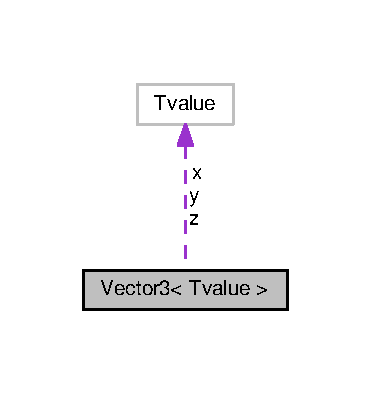
\includegraphics[width=178pt]{class_vector3__coll__graph}
\end{center}
\end{figure}
\subsection*{Public Member Functions}
\begin{DoxyCompactItemize}
\item 
\hyperlink{class_vector3_a1ab223d942be7732183ee116accb4801}{Vector3} ()
\item 
\hyperlink{class_vector3_a3edecc7c83a95dba71584e169ed0af86}{Vector3} (Tvalue xx)
\item 
\hyperlink{class_vector3_a562c9473219f42500d74662244e5c54a}{Vector3} (Tvalue xx, Tvalue yy, Tvalue zz)
\item 
\hyperlink{class_vector3}{Vector3} \& \hyperlink{class_vector3_a88f8d29ec51d966db7c36e2626040cf5}{normalize} ()
\item 
\hyperlink{class_vector3}{Vector3}$<$ Tvalue $>$ \hyperlink{class_vector3_a6f27f180b7dfa13df47fb0d5b53abc94}{operator$\ast$} (const Tvalue \&mul) const
\item 
\hyperlink{class_vector3}{Vector3}$<$ Tvalue $>$ \hyperlink{class_vector3_abf9dfd8150ddce3d68de3a05f359f8c7}{operator$\ast$} (const \hyperlink{class_vector3}{Vector3}$<$ Tvalue $>$ \&mulv) const
\item 
Tvalue \hyperlink{class_vector3_a800b81a6260784ccc20ab127833c969c}{dot} (const \hyperlink{class_vector3}{Vector3}$<$ Tvalue $>$ \&d) const
\item 
\hyperlink{class_vector3}{Vector3}$<$ Tvalue $>$ \hyperlink{class_vector3_a1ffdb538fbdeb746c34d10ccb0481691}{operator-\/} (const \hyperlink{class_vector3}{Vector3}$<$ Tvalue $>$ \&sub) const
\item 
\hyperlink{class_vector3}{Vector3}$<$ Tvalue $>$ \hyperlink{class_vector3_a69f0cdbed5fc093183e07fcc89a23136}{operator+} (const \hyperlink{class_vector3}{Vector3}$<$ Tvalue $>$ \&p) const
\item 
\hyperlink{class_vector3}{Vector3}$<$ Tvalue $>$ \& \hyperlink{class_vector3_a3e7c9473344707d60601964a20d73089}{operator+=} (const \hyperlink{class_vector3}{Vector3}$<$ Tvalue $>$ \&pe)
\item 
\hyperlink{class_vector3}{Vector3}$<$ Tvalue $>$ \& \hyperlink{class_vector3_a9e935ee74a6f8b917767b867cfa74a5d}{operator$\ast$=} (const \hyperlink{class_vector3}{Vector3}$<$ Tvalue $>$ \&mule)
\item 
\hyperlink{class_vector3}{Vector3}$<$ Tvalue $>$ \hyperlink{class_vector3_a40dd7f0f2060b7ace809dd64fe768a35}{operator-\/} () const
\item 
Tvalue \hyperlink{class_vector3_a8d6f6aa9d499d65f7e32bb88f1442aef}{length2} () const
\item 
Tvalue \hyperlink{class_vector3_a193a8d533eec9444459626e6c4faee2d}{length} () const
\end{DoxyCompactItemize}
\subsection*{Public Attributes}
\begin{DoxyCompactItemize}
\item 
Tvalue \hyperlink{class_vector3_ab6ece7df9cac25e4bf84335c4c5e2a57}{x}
\item 
Tvalue \hyperlink{class_vector3_a5742639cebe5b4750358cd08ee8835b6}{y}
\item 
Tvalue \hyperlink{class_vector3_a6d9eb4a6396bd9bbb246657b624717ae}{z}
\end{DoxyCompactItemize}
\subsection*{Friends}
\begin{DoxyCompactItemize}
\item 
std\+::ostream \& \hyperlink{class_vector3_a6faebe784277908a475d6a10cb1f45b3}{operator$<$$<$} (std\+::ostream \&os, const \hyperlink{class_vector3}{Vector3}$<$ Tvalue $>$ \&tv)
\end{DoxyCompactItemize}


\subsection{Detailed Description}
\subsubsection*{template$<$typename Tvalue$>$\newline
class Vector3$<$ Tvalue $>$}



Definition at line 14 of file Vector3.\+h.



\subsection{Constructor \& Destructor Documentation}
\mbox{\Hypertarget{class_vector3_a1ab223d942be7732183ee116accb4801}\label{class_vector3_a1ab223d942be7732183ee116accb4801}} 
\index{Vector3@{Vector3}!Vector3@{Vector3}}
\index{Vector3@{Vector3}!Vector3@{Vector3}}
\subsubsection{\texorpdfstring{Vector3()}{Vector3()}\hspace{0.1cm}{\footnotesize\ttfamily [1/3]}}
{\footnotesize\ttfamily template$<$typename Tvalue$>$ \\
\hyperlink{class_vector3}{Vector3}$<$ Tvalue $>$\+::\hyperlink{class_vector3}{Vector3} (\begin{DoxyParamCaption}{ }\end{DoxyParamCaption})\hspace{0.3cm}{\ttfamily [inline]}}



Definition at line 19 of file Vector3.\+h.

\mbox{\Hypertarget{class_vector3_a3edecc7c83a95dba71584e169ed0af86}\label{class_vector3_a3edecc7c83a95dba71584e169ed0af86}} 
\index{Vector3@{Vector3}!Vector3@{Vector3}}
\index{Vector3@{Vector3}!Vector3@{Vector3}}
\subsubsection{\texorpdfstring{Vector3()}{Vector3()}\hspace{0.1cm}{\footnotesize\ttfamily [2/3]}}
{\footnotesize\ttfamily template$<$typename Tvalue$>$ \\
\hyperlink{class_vector3}{Vector3}$<$ Tvalue $>$\+::\hyperlink{class_vector3}{Vector3} (\begin{DoxyParamCaption}\item[{Tvalue}]{xx }\end{DoxyParamCaption})\hspace{0.3cm}{\ttfamily [inline]}}



Definition at line 20 of file Vector3.\+h.

\mbox{\Hypertarget{class_vector3_a562c9473219f42500d74662244e5c54a}\label{class_vector3_a562c9473219f42500d74662244e5c54a}} 
\index{Vector3@{Vector3}!Vector3@{Vector3}}
\index{Vector3@{Vector3}!Vector3@{Vector3}}
\subsubsection{\texorpdfstring{Vector3()}{Vector3()}\hspace{0.1cm}{\footnotesize\ttfamily [3/3]}}
{\footnotesize\ttfamily template$<$typename Tvalue$>$ \\
\hyperlink{class_vector3}{Vector3}$<$ Tvalue $>$\+::\hyperlink{class_vector3}{Vector3} (\begin{DoxyParamCaption}\item[{Tvalue}]{xx,  }\item[{Tvalue}]{yy,  }\item[{Tvalue}]{zz }\end{DoxyParamCaption})\hspace{0.3cm}{\ttfamily [inline]}}



Definition at line 21 of file Vector3.\+h.



\subsection{Member Function Documentation}
\mbox{\Hypertarget{class_vector3_a800b81a6260784ccc20ab127833c969c}\label{class_vector3_a800b81a6260784ccc20ab127833c969c}} 
\index{Vector3@{Vector3}!dot@{dot}}
\index{dot@{dot}!Vector3@{Vector3}}
\subsubsection{\texorpdfstring{dot()}{dot()}}
{\footnotesize\ttfamily template$<$typename Tvalue$>$ \\
Tvalue \hyperlink{class_vector3}{Vector3}$<$ Tvalue $>$\+::dot (\begin{DoxyParamCaption}\item[{const \hyperlink{class_vector3}{Vector3}$<$ Tvalue $>$ \&}]{d }\end{DoxyParamCaption}) const\hspace{0.3cm}{\ttfamily [inline]}}



Definition at line 40 of file Vector3.\+h.

\mbox{\Hypertarget{class_vector3_a193a8d533eec9444459626e6c4faee2d}\label{class_vector3_a193a8d533eec9444459626e6c4faee2d}} 
\index{Vector3@{Vector3}!length@{length}}
\index{length@{length}!Vector3@{Vector3}}
\subsubsection{\texorpdfstring{length()}{length()}}
{\footnotesize\ttfamily template$<$typename Tvalue$>$ \\
Tvalue \hyperlink{class_vector3}{Vector3}$<$ Tvalue $>$\+::length (\begin{DoxyParamCaption}{ }\end{DoxyParamCaption}) const\hspace{0.3cm}{\ttfamily [inline]}}



Definition at line 54 of file Vector3.\+h.

\mbox{\Hypertarget{class_vector3_a8d6f6aa9d499d65f7e32bb88f1442aef}\label{class_vector3_a8d6f6aa9d499d65f7e32bb88f1442aef}} 
\index{Vector3@{Vector3}!length2@{length2}}
\index{length2@{length2}!Vector3@{Vector3}}
\subsubsection{\texorpdfstring{length2()}{length2()}}
{\footnotesize\ttfamily template$<$typename Tvalue$>$ \\
Tvalue \hyperlink{class_vector3}{Vector3}$<$ Tvalue $>$\+::length2 (\begin{DoxyParamCaption}{ }\end{DoxyParamCaption}) const\hspace{0.3cm}{\ttfamily [inline]}}



Definition at line 52 of file Vector3.\+h.

\mbox{\Hypertarget{class_vector3_a88f8d29ec51d966db7c36e2626040cf5}\label{class_vector3_a88f8d29ec51d966db7c36e2626040cf5}} 
\index{Vector3@{Vector3}!normalize@{normalize}}
\index{normalize@{normalize}!Vector3@{Vector3}}
\subsubsection{\texorpdfstring{normalize()}{normalize()}}
{\footnotesize\ttfamily template$<$typename Tvalue$>$ \\
\hyperlink{class_vector3}{Vector3}\& \hyperlink{class_vector3}{Vector3}$<$ Tvalue $>$\+::normalize (\begin{DoxyParamCaption}{ }\end{DoxyParamCaption})\hspace{0.3cm}{\ttfamily [inline]}}



Definition at line 24 of file Vector3.\+h.

\mbox{\Hypertarget{class_vector3_a6f27f180b7dfa13df47fb0d5b53abc94}\label{class_vector3_a6f27f180b7dfa13df47fb0d5b53abc94}} 
\index{Vector3@{Vector3}!operator$\ast$@{operator$\ast$}}
\index{operator$\ast$@{operator$\ast$}!Vector3@{Vector3}}
\subsubsection{\texorpdfstring{operator$\ast$()}{operator*()}\hspace{0.1cm}{\footnotesize\ttfamily [1/2]}}
{\footnotesize\ttfamily template$<$typename Tvalue$>$ \\
\hyperlink{class_vector3}{Vector3}$<$Tvalue$>$ \hyperlink{class_vector3}{Vector3}$<$ Tvalue $>$\+::operator$\ast$ (\begin{DoxyParamCaption}\item[{const Tvalue \&}]{mul }\end{DoxyParamCaption}) const\hspace{0.3cm}{\ttfamily [inline]}}



Definition at line 36 of file Vector3.\+h.

\mbox{\Hypertarget{class_vector3_abf9dfd8150ddce3d68de3a05f359f8c7}\label{class_vector3_abf9dfd8150ddce3d68de3a05f359f8c7}} 
\index{Vector3@{Vector3}!operator$\ast$@{operator$\ast$}}
\index{operator$\ast$@{operator$\ast$}!Vector3@{Vector3}}
\subsubsection{\texorpdfstring{operator$\ast$()}{operator*()}\hspace{0.1cm}{\footnotesize\ttfamily [2/2]}}
{\footnotesize\ttfamily template$<$typename Tvalue$>$ \\
\hyperlink{class_vector3}{Vector3}$<$Tvalue$>$ \hyperlink{class_vector3}{Vector3}$<$ Tvalue $>$\+::operator$\ast$ (\begin{DoxyParamCaption}\item[{const \hyperlink{class_vector3}{Vector3}$<$ Tvalue $>$ \&}]{mulv }\end{DoxyParamCaption}) const\hspace{0.3cm}{\ttfamily [inline]}}



Definition at line 38 of file Vector3.\+h.

\mbox{\Hypertarget{class_vector3_a9e935ee74a6f8b917767b867cfa74a5d}\label{class_vector3_a9e935ee74a6f8b917767b867cfa74a5d}} 
\index{Vector3@{Vector3}!operator$\ast$=@{operator$\ast$=}}
\index{operator$\ast$=@{operator$\ast$=}!Vector3@{Vector3}}
\subsubsection{\texorpdfstring{operator$\ast$=()}{operator*=()}}
{\footnotesize\ttfamily template$<$typename Tvalue$>$ \\
\hyperlink{class_vector3}{Vector3}$<$Tvalue$>$\& \hyperlink{class_vector3}{Vector3}$<$ Tvalue $>$\+::operator$\ast$= (\begin{DoxyParamCaption}\item[{const \hyperlink{class_vector3}{Vector3}$<$ Tvalue $>$ \&}]{mule }\end{DoxyParamCaption})\hspace{0.3cm}{\ttfamily [inline]}}



Definition at line 48 of file Vector3.\+h.

\mbox{\Hypertarget{class_vector3_a69f0cdbed5fc093183e07fcc89a23136}\label{class_vector3_a69f0cdbed5fc093183e07fcc89a23136}} 
\index{Vector3@{Vector3}!operator+@{operator+}}
\index{operator+@{operator+}!Vector3@{Vector3}}
\subsubsection{\texorpdfstring{operator+()}{operator+()}}
{\footnotesize\ttfamily template$<$typename Tvalue$>$ \\
\hyperlink{class_vector3}{Vector3}$<$Tvalue$>$ \hyperlink{class_vector3}{Vector3}$<$ Tvalue $>$\+::operator+ (\begin{DoxyParamCaption}\item[{const \hyperlink{class_vector3}{Vector3}$<$ Tvalue $>$ \&}]{p }\end{DoxyParamCaption}) const\hspace{0.3cm}{\ttfamily [inline]}}



Definition at line 44 of file Vector3.\+h.

\mbox{\Hypertarget{class_vector3_a3e7c9473344707d60601964a20d73089}\label{class_vector3_a3e7c9473344707d60601964a20d73089}} 
\index{Vector3@{Vector3}!operator+=@{operator+=}}
\index{operator+=@{operator+=}!Vector3@{Vector3}}
\subsubsection{\texorpdfstring{operator+=()}{operator+=()}}
{\footnotesize\ttfamily template$<$typename Tvalue$>$ \\
\hyperlink{class_vector3}{Vector3}$<$Tvalue$>$\& \hyperlink{class_vector3}{Vector3}$<$ Tvalue $>$\+::operator+= (\begin{DoxyParamCaption}\item[{const \hyperlink{class_vector3}{Vector3}$<$ Tvalue $>$ \&}]{pe }\end{DoxyParamCaption})\hspace{0.3cm}{\ttfamily [inline]}}



Definition at line 46 of file Vector3.\+h.

\mbox{\Hypertarget{class_vector3_a1ffdb538fbdeb746c34d10ccb0481691}\label{class_vector3_a1ffdb538fbdeb746c34d10ccb0481691}} 
\index{Vector3@{Vector3}!operator-\/@{operator-\/}}
\index{operator-\/@{operator-\/}!Vector3@{Vector3}}
\subsubsection{\texorpdfstring{operator-\/()}{operator-()}\hspace{0.1cm}{\footnotesize\ttfamily [1/2]}}
{\footnotesize\ttfamily template$<$typename Tvalue$>$ \\
\hyperlink{class_vector3}{Vector3}$<$Tvalue$>$ \hyperlink{class_vector3}{Vector3}$<$ Tvalue $>$\+::operator-\/ (\begin{DoxyParamCaption}\item[{const \hyperlink{class_vector3}{Vector3}$<$ Tvalue $>$ \&}]{sub }\end{DoxyParamCaption}) const\hspace{0.3cm}{\ttfamily [inline]}}



Definition at line 42 of file Vector3.\+h.

\mbox{\Hypertarget{class_vector3_a40dd7f0f2060b7ace809dd64fe768a35}\label{class_vector3_a40dd7f0f2060b7ace809dd64fe768a35}} 
\index{Vector3@{Vector3}!operator-\/@{operator-\/}}
\index{operator-\/@{operator-\/}!Vector3@{Vector3}}
\subsubsection{\texorpdfstring{operator-\/()}{operator-()}\hspace{0.1cm}{\footnotesize\ttfamily [2/2]}}
{\footnotesize\ttfamily template$<$typename Tvalue$>$ \\
\hyperlink{class_vector3}{Vector3}$<$Tvalue$>$ \hyperlink{class_vector3}{Vector3}$<$ Tvalue $>$\+::operator-\/ (\begin{DoxyParamCaption}{ }\end{DoxyParamCaption}) const\hspace{0.3cm}{\ttfamily [inline]}}



Definition at line 50 of file Vector3.\+h.



\subsection{Friends And Related Function Documentation}
\mbox{\Hypertarget{class_vector3_a6faebe784277908a475d6a10cb1f45b3}\label{class_vector3_a6faebe784277908a475d6a10cb1f45b3}} 
\index{Vector3@{Vector3}!operator$<$$<$@{operator$<$$<$}}
\index{operator$<$$<$@{operator$<$$<$}!Vector3@{Vector3}}
\subsubsection{\texorpdfstring{operator$<$$<$}{operator<<}}
{\footnotesize\ttfamily template$<$typename Tvalue$>$ \\
std\+::ostream\& operator$<$$<$ (\begin{DoxyParamCaption}\item[{std\+::ostream \&}]{os,  }\item[{const \hyperlink{class_vector3}{Vector3}$<$ Tvalue $>$ \&}]{tv }\end{DoxyParamCaption})\hspace{0.3cm}{\ttfamily [friend]}}



Definition at line 56 of file Vector3.\+h.



\subsection{Member Data Documentation}
\mbox{\Hypertarget{class_vector3_ab6ece7df9cac25e4bf84335c4c5e2a57}\label{class_vector3_ab6ece7df9cac25e4bf84335c4c5e2a57}} 
\index{Vector3@{Vector3}!x@{x}}
\index{x@{x}!Vector3@{Vector3}}
\subsubsection{\texorpdfstring{x}{x}}
{\footnotesize\ttfamily template$<$typename Tvalue$>$ \\
Tvalue \hyperlink{class_vector3}{Vector3}$<$ Tvalue $>$\+::x}



Definition at line 18 of file Vector3.\+h.

\mbox{\Hypertarget{class_vector3_a5742639cebe5b4750358cd08ee8835b6}\label{class_vector3_a5742639cebe5b4750358cd08ee8835b6}} 
\index{Vector3@{Vector3}!y@{y}}
\index{y@{y}!Vector3@{Vector3}}
\subsubsection{\texorpdfstring{y}{y}}
{\footnotesize\ttfamily template$<$typename Tvalue$>$ \\
Tvalue \hyperlink{class_vector3}{Vector3}$<$ Tvalue $>$\+::y}



Definition at line 18 of file Vector3.\+h.

\mbox{\Hypertarget{class_vector3_a6d9eb4a6396bd9bbb246657b624717ae}\label{class_vector3_a6d9eb4a6396bd9bbb246657b624717ae}} 
\index{Vector3@{Vector3}!z@{z}}
\index{z@{z}!Vector3@{Vector3}}
\subsubsection{\texorpdfstring{z}{z}}
{\footnotesize\ttfamily template$<$typename Tvalue$>$ \\
Tvalue \hyperlink{class_vector3}{Vector3}$<$ Tvalue $>$\+::z}



Definition at line 18 of file Vector3.\+h.



The documentation for this class was generated from the following file\+:\begin{DoxyCompactItemize}
\item 
/home/rory/\+Projects/ece-\/6122-\/final-\/project/src/raytracer/\hyperlink{_vector3_8h}{Vector3.\+h}\end{DoxyCompactItemize}

\hypertarget{struct_vertex}{}\section{Vertex Struct Reference}
\label{struct_vertex}\index{Vertex@{Vertex}}


{\ttfamily \#include $<$Vertex.\+h$>$}

\subsection*{Public Member Functions}
\begin{DoxyCompactItemize}
\item 
\hyperlink{struct_vertex_a97488994a2482d70da74e1b91d40e169}{Vertex} ()
\item 
\hyperlink{struct_vertex_a30e022efb3a5d01ab1e1451ca871264e}{Vertex} (glm\+::vec4 \hyperlink{struct_vertex_a6814af2586248942604e8edd28d950a9}{position}, glm\+::vec2 \hyperlink{struct_vertex_a8d5cc8548016889746f251d98377ec8a}{uv}, glm\+::vec4 \hyperlink{struct_vertex_aa7ecd21578677765699b8831e0011696}{color}, glm\+::vec3 \hyperlink{struct_vertex_a3aa35fe84025ecf1acccb5f65f5577fd}{normal})
\item 
\hyperlink{struct_vertex_a2947e9185be83a2142f5676ed101d727}{Vertex} (float x, float y, float z, float w, float u, float v, float r, float g, float b, float a, float m, float n, float o)
\end{DoxyCompactItemize}
\subsection*{Public Attributes}
\begin{DoxyCompactItemize}
\item 
glm\+::vec4 \hyperlink{struct_vertex_a6814af2586248942604e8edd28d950a9}{position}
\item 
glm\+::vec2 \hyperlink{struct_vertex_a8d5cc8548016889746f251d98377ec8a}{uv}
\item 
glm\+::vec4 \hyperlink{struct_vertex_aa7ecd21578677765699b8831e0011696}{color}
\item 
glm\+::vec3 \hyperlink{struct_vertex_a3aa35fe84025ecf1acccb5f65f5577fd}{normal}
\end{DoxyCompactItemize}


\subsection{Detailed Description}


Definition at line 8 of file Vertex.\+h.



\subsection{Constructor \& Destructor Documentation}
\mbox{\Hypertarget{struct_vertex_a97488994a2482d70da74e1b91d40e169}\label{struct_vertex_a97488994a2482d70da74e1b91d40e169}} 
\index{Vertex@{Vertex}!Vertex@{Vertex}}
\index{Vertex@{Vertex}!Vertex@{Vertex}}
\subsubsection{\texorpdfstring{Vertex()}{Vertex()}\hspace{0.1cm}{\footnotesize\ttfamily [1/3]}}
{\footnotesize\ttfamily Vertex\+::\+Vertex (\begin{DoxyParamCaption}{ }\end{DoxyParamCaption})}

Constructor 

Definition at line 6 of file Vertex.\+cpp.

\mbox{\Hypertarget{struct_vertex_a30e022efb3a5d01ab1e1451ca871264e}\label{struct_vertex_a30e022efb3a5d01ab1e1451ca871264e}} 
\index{Vertex@{Vertex}!Vertex@{Vertex}}
\index{Vertex@{Vertex}!Vertex@{Vertex}}
\subsubsection{\texorpdfstring{Vertex()}{Vertex()}\hspace{0.1cm}{\footnotesize\ttfamily [2/3]}}
{\footnotesize\ttfamily Vertex\+::\+Vertex (\begin{DoxyParamCaption}\item[{glm\+::vec4}]{position,  }\item[{glm\+::vec2}]{uv,  }\item[{glm\+::vec4}]{color,  }\item[{glm\+::vec3}]{normal }\end{DoxyParamCaption})}

Constructor 
\begin{DoxyParams}{Parameters}
{\em position} & The vertex position in model space \\
\hline
{\em uv} & The texture coordinate mapping for this vertex \\
\hline
{\em color} & The color of this vertex \\
\hline
{\em normal} & The normal for this vertex \\
\hline
\end{DoxyParams}


Definition at line 21 of file Vertex.\+cpp.

\mbox{\Hypertarget{struct_vertex_a2947e9185be83a2142f5676ed101d727}\label{struct_vertex_a2947e9185be83a2142f5676ed101d727}} 
\index{Vertex@{Vertex}!Vertex@{Vertex}}
\index{Vertex@{Vertex}!Vertex@{Vertex}}
\subsubsection{\texorpdfstring{Vertex()}{Vertex()}\hspace{0.1cm}{\footnotesize\ttfamily [3/3]}}
{\footnotesize\ttfamily Vertex\+::\+Vertex (\begin{DoxyParamCaption}\item[{float}]{x,  }\item[{float}]{y,  }\item[{float}]{z,  }\item[{float}]{w,  }\item[{float}]{u,  }\item[{float}]{v,  }\item[{float}]{r,  }\item[{float}]{g,  }\item[{float}]{b,  }\item[{float}]{a,  }\item[{float}]{m,  }\item[{float}]{n,  }\item[{float}]{o }\end{DoxyParamCaption})}

Constructor 
\begin{DoxyParams}{Parameters}
{\em x} & \hyperlink{struct_position}{Position} in x-\/direction \\
\hline
{\em y} & \hyperlink{struct_position}{Position} in y-\/direction \\
\hline
{\em z} & \hyperlink{struct_position}{Position} in z-\/direction \\
\hline
{\em w} & 1 means a point, 0 means a vector (usually=1) \\
\hline
{\em u} & \hyperlink{class_texture}{Texture} coordinate in x-\/direction \\
\hline
{\em v} & \hyperlink{class_texture}{Texture} coordinate in y-\/direction \\
\hline
{\em r} & Red color value \\
\hline
{\em g} & Green color value \\
\hline
{\em b} & Blue color value \\
\hline
{\em a} & Alpha value \\
\hline
{\em m} & \hyperlink{struct_normal}{Normal} coordinate in x-\/direction \\
\hline
{\em n} & \hyperlink{struct_normal}{Normal} coordinate in y-\/direction \\
\hline
{\em o} & \hyperlink{struct_normal}{Normal} coordinate in z-\/direction \\
\hline
\end{DoxyParams}


Definition at line 45 of file Vertex.\+cpp.



\subsection{Member Data Documentation}
\mbox{\Hypertarget{struct_vertex_aa7ecd21578677765699b8831e0011696}\label{struct_vertex_aa7ecd21578677765699b8831e0011696}} 
\index{Vertex@{Vertex}!color@{color}}
\index{color@{color}!Vertex@{Vertex}}
\subsubsection{\texorpdfstring{color}{color}}
{\footnotesize\ttfamily glm\+::vec4 Vertex\+::color}



Definition at line 13 of file Vertex.\+h.

\mbox{\Hypertarget{struct_vertex_a3aa35fe84025ecf1acccb5f65f5577fd}\label{struct_vertex_a3aa35fe84025ecf1acccb5f65f5577fd}} 
\index{Vertex@{Vertex}!normal@{normal}}
\index{normal@{normal}!Vertex@{Vertex}}
\subsubsection{\texorpdfstring{normal}{normal}}
{\footnotesize\ttfamily glm\+::vec3 Vertex\+::normal}



Definition at line 14 of file Vertex.\+h.

\mbox{\Hypertarget{struct_vertex_a6814af2586248942604e8edd28d950a9}\label{struct_vertex_a6814af2586248942604e8edd28d950a9}} 
\index{Vertex@{Vertex}!position@{position}}
\index{position@{position}!Vertex@{Vertex}}
\subsubsection{\texorpdfstring{position}{position}}
{\footnotesize\ttfamily glm\+::vec4 Vertex\+::position}



Definition at line 10 of file Vertex.\+h.

\mbox{\Hypertarget{struct_vertex_a8d5cc8548016889746f251d98377ec8a}\label{struct_vertex_a8d5cc8548016889746f251d98377ec8a}} 
\index{Vertex@{Vertex}!uv@{uv}}
\index{uv@{uv}!Vertex@{Vertex}}
\subsubsection{\texorpdfstring{uv}{uv}}
{\footnotesize\ttfamily glm\+::vec2 Vertex\+::uv}



Definition at line 11 of file Vertex.\+h.



The documentation for this struct was generated from the following files\+:\begin{DoxyCompactItemize}
\item 
/home/rory/\+Projects/ece-\/6122-\/final-\/project/src/\hyperlink{_vertex_8h}{Vertex.\+h}\item 
/home/rory/\+Projects/ece-\/6122-\/final-\/project/src/\hyperlink{_vertex_8cpp}{Vertex.\+cpp}\end{DoxyCompactItemize}

\hypertarget{class_window}{}\section{Window Class Reference}
\label{class_window}\index{Window@{Window}}


{\ttfamily \#include $<$Window.\+h$>$}

\subsection*{Public Member Functions}
\begin{DoxyCompactItemize}
\item 
\hyperlink{class_window_a315084d17424d10fe4a77c581084b65a}{Window} (const char $\ast$title, int width, int height)
\item 
\hyperlink{class_window_a245d821e6016fa1f6970ccbbedd635f6}{$\sim$\+Window} ()
\item 
void \hyperlink{class_window_a38bc43bdd1a97e5de7f346ba4c3957ef}{clear} ()
\item 
void \hyperlink{class_window_a59515fc5a56e86d5a46d771595daac55}{update} ()
\item 
double \hyperlink{class_window_a8a828ebd82becbc53c7754916be02b79}{get\+Time} ()
\item 
bool \hyperlink{class_window_a1caaf150558c0c35a8811f19ccac817d}{should\+Close} () const
\item 
void \hyperlink{class_window_a35055c04498121d39741bfcd5082705b}{close} ()
\item 
int \hyperlink{class_window_aee31a875d654a8c8f7d796d072657791}{get\+Width} () const
\item 
int \hyperlink{class_window_a60757b2b0dbcec9889e3a09f5655adbe}{get\+Height} () const
\item 
glm\+::vec2 \hyperlink{class_window_ab276bf3630d294d6eee8c5992b93e721}{get\+Cursor\+Pos} () const
\end{DoxyCompactItemize}


\subsection{Detailed Description}


Definition at line 8 of file Window.\+h.



\subsection{Constructor \& Destructor Documentation}
\mbox{\Hypertarget{class_window_a315084d17424d10fe4a77c581084b65a}\label{class_window_a315084d17424d10fe4a77c581084b65a}} 
\index{Window@{Window}!Window@{Window}}
\index{Window@{Window}!Window@{Window}}
\subsubsection{\texorpdfstring{Window()}{Window()}}
{\footnotesize\ttfamily Window\+::\+Window (\begin{DoxyParamCaption}\item[{const char $\ast$}]{title,  }\item[{int}]{width,  }\item[{int}]{height }\end{DoxyParamCaption})}

Constructor 
\begin{DoxyParams}{Parameters}
{\em title} & The window title \\
\hline
{\em width} & The width of the window in pixels \\
\hline
{\em height} & T\+He height of the window in pixels \\
\hline
\end{DoxyParams}


Definition at line 11 of file Window.\+cpp.

\mbox{\Hypertarget{class_window_a245d821e6016fa1f6970ccbbedd635f6}\label{class_window_a245d821e6016fa1f6970ccbbedd635f6}} 
\index{Window@{Window}!````~Window@{$\sim$\+Window}}
\index{````~Window@{$\sim$\+Window}!Window@{Window}}
\subsubsection{\texorpdfstring{$\sim$\+Window()}{~Window()}}
{\footnotesize\ttfamily Window\+::$\sim$\+Window (\begin{DoxyParamCaption}{ }\end{DoxyParamCaption})}

Destructor 

Definition at line 71 of file Window.\+cpp.



\subsection{Member Function Documentation}
\mbox{\Hypertarget{class_window_a38bc43bdd1a97e5de7f346ba4c3957ef}\label{class_window_a38bc43bdd1a97e5de7f346ba4c3957ef}} 
\index{Window@{Window}!clear@{clear}}
\index{clear@{clear}!Window@{Window}}
\subsubsection{\texorpdfstring{clear()}{clear()}}
{\footnotesize\ttfamily void Window\+::clear (\begin{DoxyParamCaption}{ }\end{DoxyParamCaption})}



Definition at line 77 of file Window.\+cpp.

\mbox{\Hypertarget{class_window_a35055c04498121d39741bfcd5082705b}\label{class_window_a35055c04498121d39741bfcd5082705b}} 
\index{Window@{Window}!close@{close}}
\index{close@{close}!Window@{Window}}
\subsubsection{\texorpdfstring{close()}{close()}}
{\footnotesize\ttfamily void Window\+::close (\begin{DoxyParamCaption}{ }\end{DoxyParamCaption})}

Sets the flag to close the window 

Definition at line 135 of file Window.\+cpp.

\mbox{\Hypertarget{class_window_ab276bf3630d294d6eee8c5992b93e721}\label{class_window_ab276bf3630d294d6eee8c5992b93e721}} 
\index{Window@{Window}!get\+Cursor\+Pos@{get\+Cursor\+Pos}}
\index{get\+Cursor\+Pos@{get\+Cursor\+Pos}!Window@{Window}}
\subsubsection{\texorpdfstring{get\+Cursor\+Pos()}{getCursorPos()}}
{\footnotesize\ttfamily glm\+::vec2 Window\+::get\+Cursor\+Pos (\begin{DoxyParamCaption}{ }\end{DoxyParamCaption}) const\hspace{0.3cm}{\ttfamily [inline]}}



Definition at line 23 of file Window.\+h.

\mbox{\Hypertarget{class_window_a60757b2b0dbcec9889e3a09f5655adbe}\label{class_window_a60757b2b0dbcec9889e3a09f5655adbe}} 
\index{Window@{Window}!get\+Height@{get\+Height}}
\index{get\+Height@{get\+Height}!Window@{Window}}
\subsubsection{\texorpdfstring{get\+Height()}{getHeight()}}
{\footnotesize\ttfamily int Window\+::get\+Height (\begin{DoxyParamCaption}{ }\end{DoxyParamCaption}) const\hspace{0.3cm}{\ttfamily [inline]}}



Definition at line 22 of file Window.\+h.

\mbox{\Hypertarget{class_window_a8a828ebd82becbc53c7754916be02b79}\label{class_window_a8a828ebd82becbc53c7754916be02b79}} 
\index{Window@{Window}!get\+Time@{get\+Time}}
\index{get\+Time@{get\+Time}!Window@{Window}}
\subsubsection{\texorpdfstring{get\+Time()}{getTime()}}
{\footnotesize\ttfamily double Window\+::get\+Time (\begin{DoxyParamCaption}{ }\end{DoxyParamCaption})}

Returns a double representing the current timestamp \begin{DoxyReturn}{Returns}

\end{DoxyReturn}


Definition at line 221 of file Window.\+cpp.

\mbox{\Hypertarget{class_window_aee31a875d654a8c8f7d796d072657791}\label{class_window_aee31a875d654a8c8f7d796d072657791}} 
\index{Window@{Window}!get\+Width@{get\+Width}}
\index{get\+Width@{get\+Width}!Window@{Window}}
\subsubsection{\texorpdfstring{get\+Width()}{getWidth()}}
{\footnotesize\ttfamily int Window\+::get\+Width (\begin{DoxyParamCaption}{ }\end{DoxyParamCaption}) const\hspace{0.3cm}{\ttfamily [inline]}}



Definition at line 21 of file Window.\+h.

\mbox{\Hypertarget{class_window_a1caaf150558c0c35a8811f19ccac817d}\label{class_window_a1caaf150558c0c35a8811f19ccac817d}} 
\index{Window@{Window}!should\+Close@{should\+Close}}
\index{should\+Close@{should\+Close}!Window@{Window}}
\subsubsection{\texorpdfstring{should\+Close()}{shouldClose()}}
{\footnotesize\ttfamily bool Window\+::should\+Close (\begin{DoxyParamCaption}{ }\end{DoxyParamCaption}) const}

Returns whether the window is set to close or not \begin{DoxyReturn}{Returns}
Returns T\+R\+UE if the window is set to close, else F\+A\+L\+SE 
\end{DoxyReturn}


Definition at line 127 of file Window.\+cpp.

\mbox{\Hypertarget{class_window_a59515fc5a56e86d5a46d771595daac55}\label{class_window_a59515fc5a56e86d5a46d771595daac55}} 
\index{Window@{Window}!update@{update}}
\index{update@{update}!Window@{Window}}
\subsubsection{\texorpdfstring{update()}{update()}}
{\footnotesize\ttfamily void Window\+::update (\begin{DoxyParamCaption}{ }\end{DoxyParamCaption})}

Checks for Open\+GL errors, updates input events, and draws the window buffer 

Definition at line 85 of file Window.\+cpp.



The documentation for this class was generated from the following files\+:\begin{DoxyCompactItemize}
\item 
/home/rory/\+Projects/ece-\/6122-\/final-\/project/src/\hyperlink{_window_8h}{Window.\+h}\item 
/home/rory/\+Projects/ece-\/6122-\/final-\/project/src/\hyperlink{_window_8cpp}{Window.\+cpp}\end{DoxyCompactItemize}

\chapter{File Documentation}
\hypertarget{_arg_parser_8h}{}\section{/home/rory/\+Projects/ece-\/6122-\/final-\/project/src/\+Arg\+Parser.h File Reference}
\label{_arg_parser_8h}\index{/home/rory/\+Projects/ece-\/6122-\/final-\/project/src/\+Arg\+Parser.\+h@{/home/rory/\+Projects/ece-\/6122-\/final-\/project/src/\+Arg\+Parser.\+h}}
{\ttfamily \#include \char`\"{}Program\+Config.\+h\char`\"{}}\newline
{\ttfamily \#include $<$getopt.\+h$>$}\newline
{\ttfamily \#include $<$cstdio$>$}\newline
{\ttfamily \#include $<$cstdlib$>$}\newline
Include dependency graph for Arg\+Parser.\+h\+:
\nopagebreak
\begin{figure}[H]
\begin{center}
\leavevmode
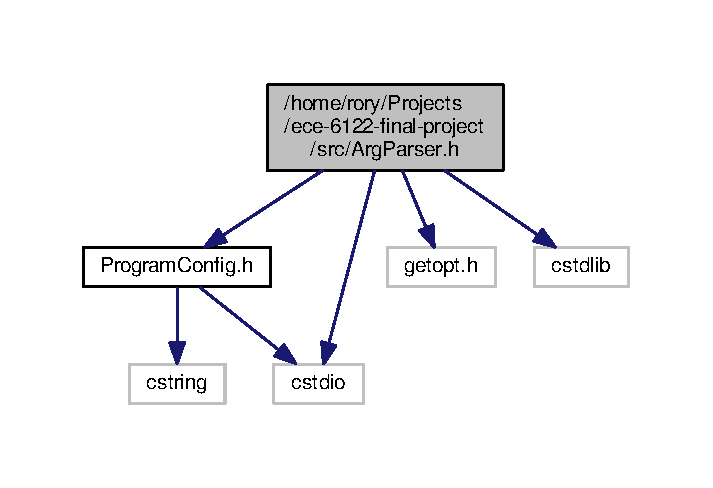
\includegraphics[width=342pt]{_arg_parser_8h__incl}
\end{center}
\end{figure}
This graph shows which files directly or indirectly include this file\+:
\nopagebreak
\begin{figure}[H]
\begin{center}
\leavevmode
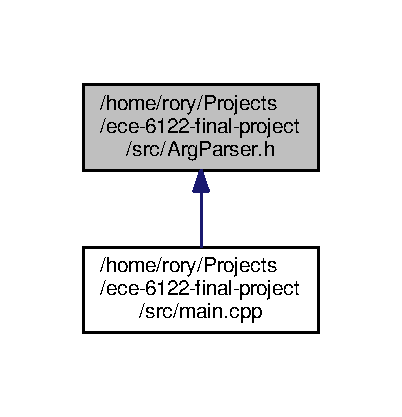
\includegraphics[width=193pt]{_arg_parser_8h__dep__incl}
\end{center}
\end{figure}
\subsection*{Classes}
\begin{DoxyCompactItemize}
\item 
class \hyperlink{class_arg_parser}{Arg\+Parser}
\end{DoxyCompactItemize}
\subsection*{Macros}
\begin{DoxyCompactItemize}
\item 
\#define \hyperlink{_arg_parser_8h_a2a60136d5d0829a8be576e2779f885d6}{H\+E\+L\+P\+\_\+\+A\+RG}~1000
\end{DoxyCompactItemize}


\subsection{Macro Definition Documentation}
\mbox{\Hypertarget{_arg_parser_8h_a2a60136d5d0829a8be576e2779f885d6}\label{_arg_parser_8h_a2a60136d5d0829a8be576e2779f885d6}} 
\index{Arg\+Parser.\+h@{Arg\+Parser.\+h}!H\+E\+L\+P\+\_\+\+A\+RG@{H\+E\+L\+P\+\_\+\+A\+RG}}
\index{H\+E\+L\+P\+\_\+\+A\+RG@{H\+E\+L\+P\+\_\+\+A\+RG}!Arg\+Parser.\+h@{Arg\+Parser.\+h}}
\subsubsection{\texorpdfstring{H\+E\+L\+P\+\_\+\+A\+RG}{HELP\_ARG}}
{\footnotesize\ttfamily \#define H\+E\+L\+P\+\_\+\+A\+RG~1000}



Definition at line 9 of file Arg\+Parser.\+h.


\hypertarget{_layer_8cpp}{}\section{/home/rory/\+Projects/ece-\/6122-\/final-\/project/src/\+Layer.cpp File Reference}
\label{_layer_8cpp}\index{/home/rory/\+Projects/ece-\/6122-\/final-\/project/src/\+Layer.\+cpp@{/home/rory/\+Projects/ece-\/6122-\/final-\/project/src/\+Layer.\+cpp}}
{\ttfamily \#include \char`\"{}Layer.\+h\char`\"{}}\newline
Include dependency graph for Layer.\+cpp\+:
\nopagebreak
\begin{figure}[H]
\begin{center}
\leavevmode
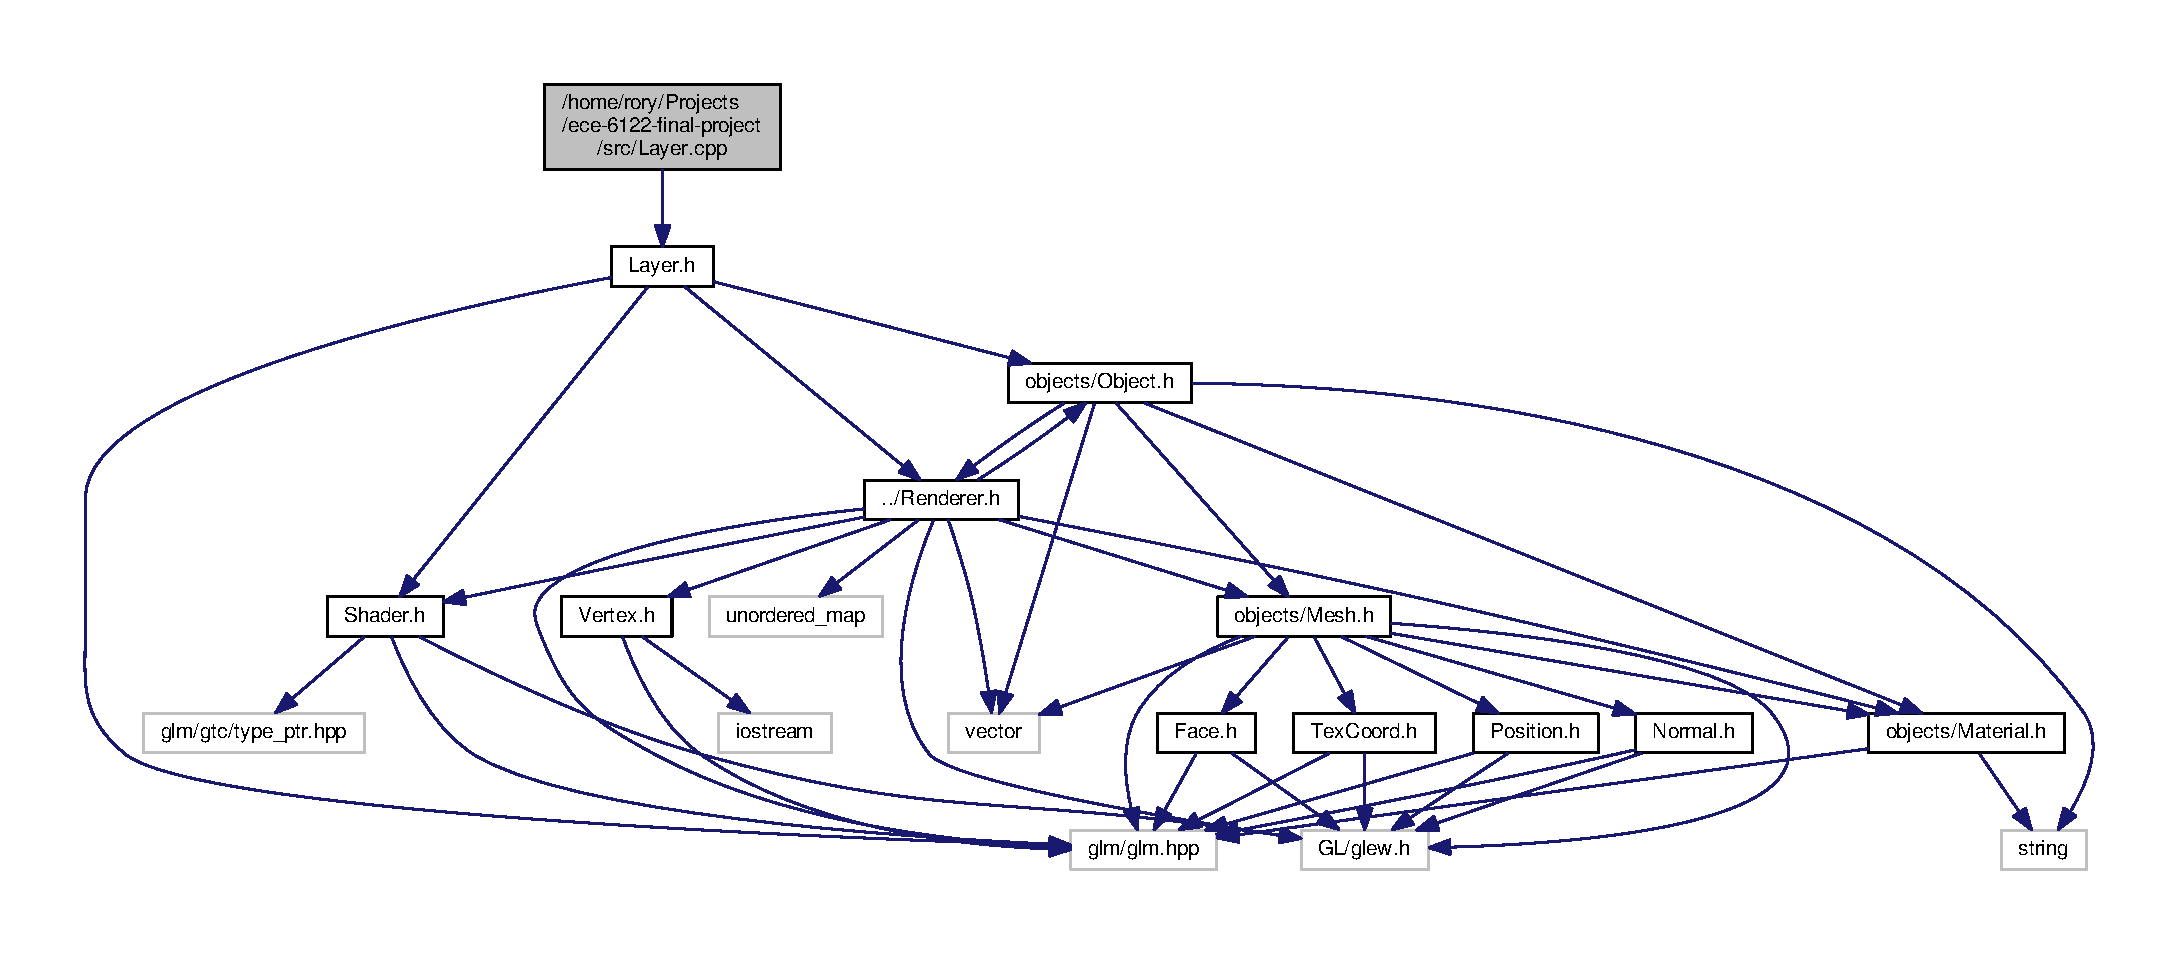
\includegraphics[width=350pt]{_layer_8cpp__incl}
\end{center}
\end{figure}

\hypertarget{_layer_8h}{}\section{/home/rory/\+Projects/ece-\/6122-\/final-\/project/src/\+Layer.h File Reference}
\label{_layer_8h}\index{/home/rory/\+Projects/ece-\/6122-\/final-\/project/src/\+Layer.\+h@{/home/rory/\+Projects/ece-\/6122-\/final-\/project/src/\+Layer.\+h}}
{\ttfamily \#include \char`\"{}objects/\+Object.\+h\char`\"{}}\newline
{\ttfamily \#include \char`\"{}Renderer.\+h\char`\"{}}\newline
{\ttfamily \#include \char`\"{}Shader.\+h\char`\"{}}\newline
{\ttfamily \#include $<$glm/glm.\+hpp$>$}\newline
Include dependency graph for Layer.\+h\+:
\nopagebreak
\begin{figure}[H]
\begin{center}
\leavevmode
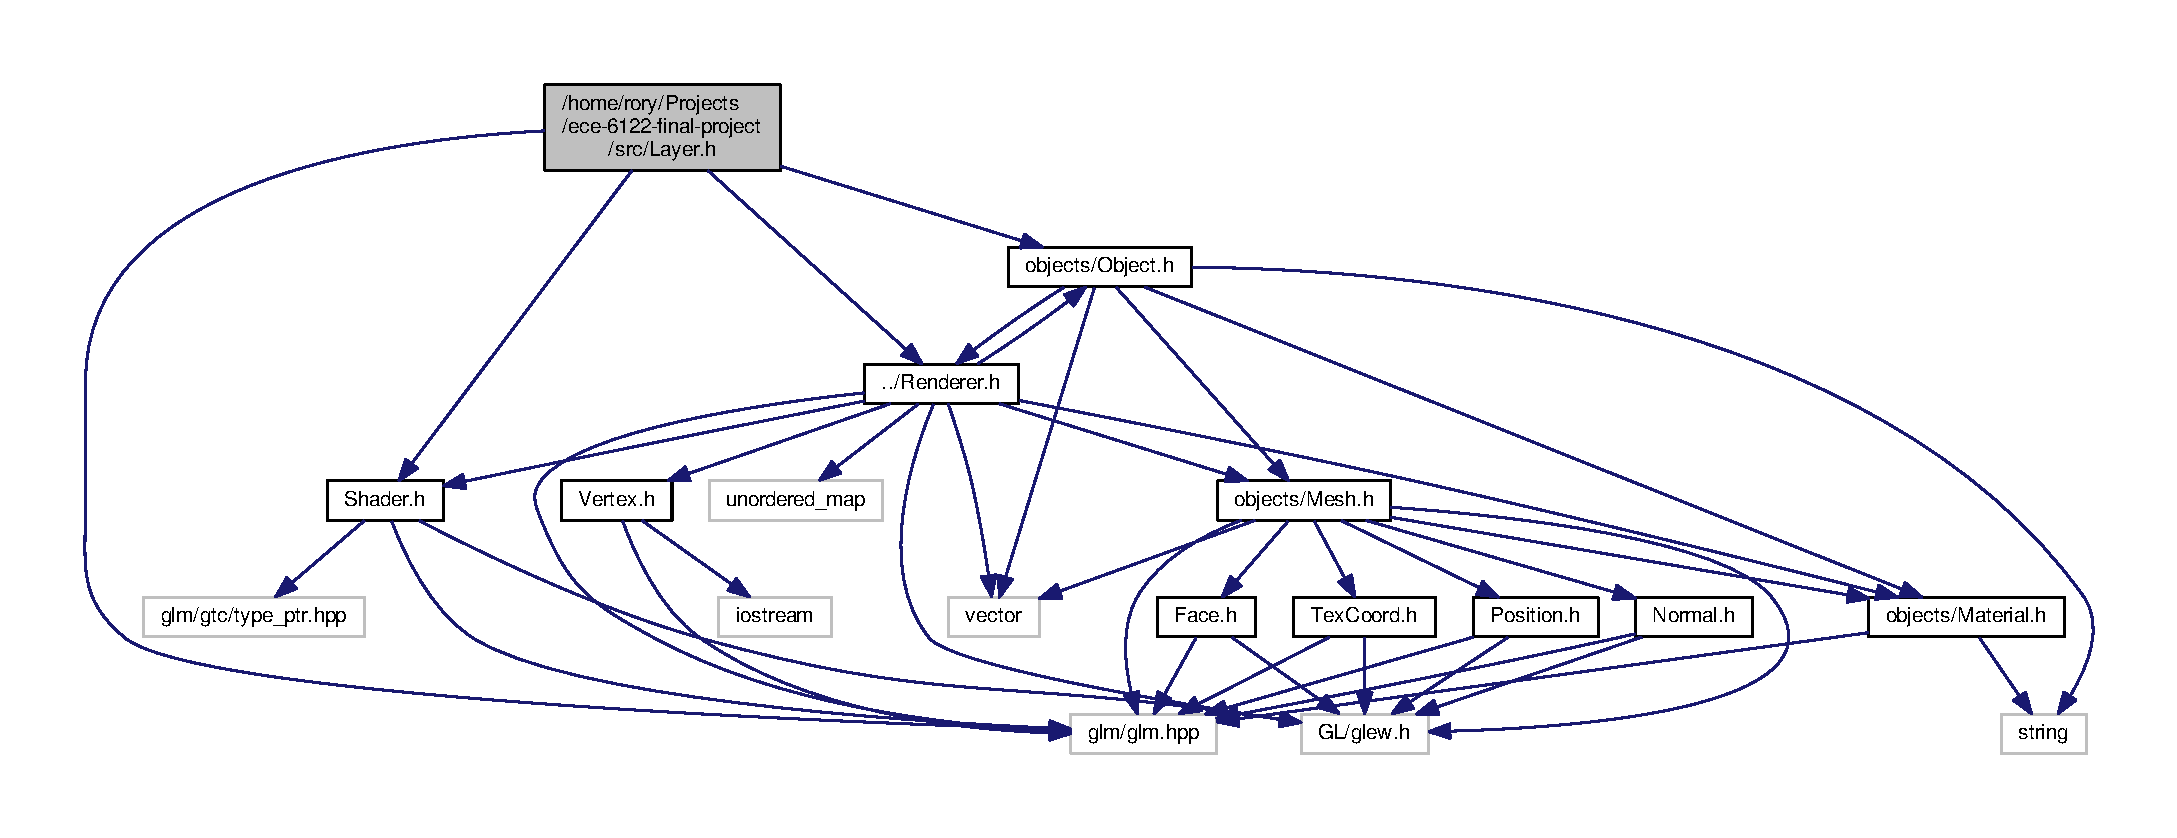
\includegraphics[width=350pt]{_layer_8h__incl}
\end{center}
\end{figure}
This graph shows which files directly or indirectly include this file\+:
\nopagebreak
\begin{figure}[H]
\begin{center}
\leavevmode
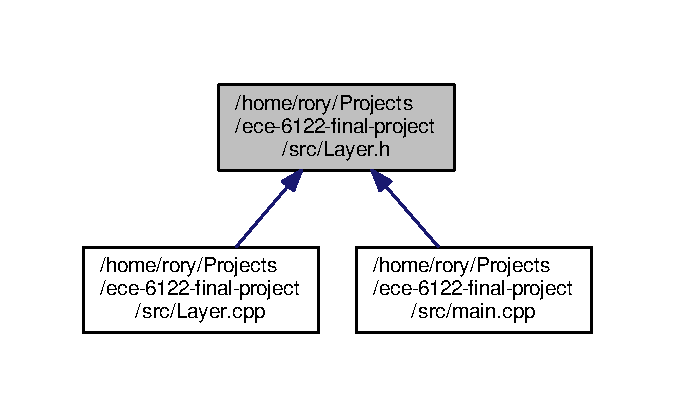
\includegraphics[width=324pt]{_layer_8h__dep__incl}
\end{center}
\end{figure}
\subsection*{Classes}
\begin{DoxyCompactItemize}
\item 
class \hyperlink{class_layer}{Layer}
\end{DoxyCompactItemize}

\hypertarget{main_8cpp}{}\section{/home/rory/\+Projects/ece-\/6122-\/final-\/project/src/main.cpp File Reference}
\label{main_8cpp}\index{/home/rory/\+Projects/ece-\/6122-\/final-\/project/src/main.\+cpp@{/home/rory/\+Projects/ece-\/6122-\/final-\/project/src/main.\+cpp}}
{\ttfamily \#include \char`\"{}Arg\+Parser.\+h\char`\"{}}\newline
{\ttfamily \#include \char`\"{}Window.\+h\char`\"{}}\newline
{\ttfamily \#include \char`\"{}Physics\+Engine.\+h\char`\"{}}\newline
{\ttfamily \#include \char`\"{}Shader.\+h\char`\"{}}\newline
{\ttfamily \#include \char`\"{}Text\+Writer.\+h\char`\"{}}\newline
{\ttfamily \#include \char`\"{}Layer.\+h\char`\"{}}\newline
{\ttfamily \#include \char`\"{}utils/\+Glm\+Utils.\+h\char`\"{}}\newline
{\ttfamily \#include \char`\"{}raytracer/\+Raytracer.\+h\char`\"{}}\newline
{\ttfamily \#include \char`\"{}Performance\+Data.\+h\char`\"{}}\newline
{\ttfamily \#include $<$glm/glm.\+hpp$>$}\newline
{\ttfamily \#include $<$glm/gtc/matrix\+\_\+transform.\+hpp$>$}\newline
{\ttfamily \#include $<$glm/gtx/transform.\+hpp$>$}\newline
{\ttfamily \#include $<$iostream$>$}\newline
Include dependency graph for main.\+cpp\+:
\nopagebreak
\begin{figure}[H]
\begin{center}
\leavevmode
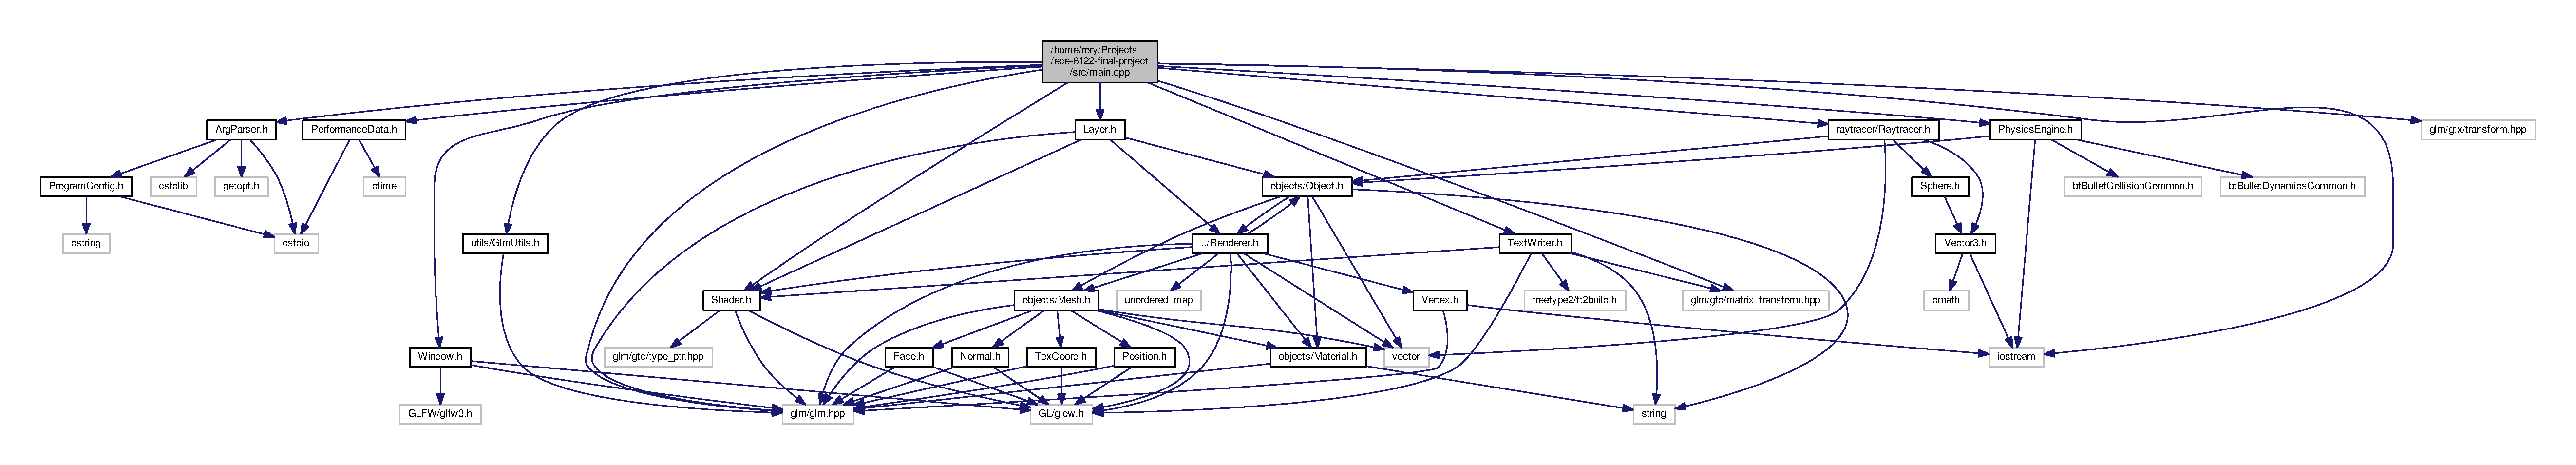
\includegraphics[width=350pt]{main_8cpp__incl}
\end{center}
\end{figure}
\subsection*{Classes}
\begin{DoxyCompactItemize}
\item 
struct \hyperlink{structobj_metadata}{obj\+Metadata}
\end{DoxyCompactItemize}
\subsection*{Macros}
\begin{DoxyCompactItemize}
\item 
\#define \hyperlink{main_8cpp_a3ca3e9eda52e6a7fc5790d61f9427647}{V\+E\+R\+T\+E\+X\+\_\+\+S\+H\+A\+D\+E\+R\+\_\+\+P\+A\+TH}~\char`\"{}../shaders/vertex.\+glsl\char`\"{}
\item 
\#define \hyperlink{main_8cpp_a21b357a3c758d8a1825fe0b84aca77b7}{F\+R\+A\+G\+M\+E\+N\+T\+\_\+\+S\+H\+A\+D\+E\+R\+\_\+\+P\+A\+TH}~\char`\"{}../shaders/fragment.\+glsl\char`\"{}
\item 
\#define \hyperlink{main_8cpp_a498d9f026138406895e9a34b504ac6a6}{W\+I\+N\+D\+O\+W\+\_\+\+W\+I\+D\+TH}~800
\item 
\#define \hyperlink{main_8cpp_a5473cf64fa979b48335079c99532e243}{W\+I\+N\+D\+O\+W\+\_\+\+H\+E\+I\+G\+HT}~600
\item 
\#define \hyperlink{main_8cpp_a3adf7b7b13572f2baf3379a8f2f4220a}{W\+I\+N\+D\+O\+W\+\_\+\+T\+I\+T\+LE}~\char`\"{}E\+C\+E6122 Final Project\char`\"{}
\end{DoxyCompactItemize}
\subsection*{Enumerations}
\begin{DoxyCompactItemize}
\item 
enum \hyperlink{main_8cpp_a5a4538eeab397888d88a4eefcc5a1345}{Shape\+Type} \{ \newline
\hyperlink{main_8cpp_a5a4538eeab397888d88a4eefcc5a1345a3cfce651e667ab85486dd42a8185f98a}{Shape\+Type\+::\+Box}, 
\hyperlink{main_8cpp_a5a4538eeab397888d88a4eefcc5a1345ab7095f057db3fefa7325ad93a04e14fd}{Shape\+Type\+::\+Sphere}, 
\hyperlink{main_8cpp_a5a4538eeab397888d88a4eefcc5a1345a2ec2c2961c7ce5a114d969c1f562a563}{Shape\+Type\+::\+Cylinder}, 
\hyperlink{main_8cpp_a5a4538eeab397888d88a4eefcc5a1345acd2c8bc6e5f1ea17c918ccaf89660104}{Shape\+Type\+::\+Cone}, 
\newline
\hyperlink{main_8cpp_a5a4538eeab397888d88a4eefcc5a1345a90589c47f06eb971d548591f23c285af}{Shape\+Type\+::\+Custom}
 \}
\end{DoxyCompactItemize}
\subsection*{Functions}
\begin{DoxyCompactItemize}
\item 
int \hyperlink{main_8cpp_a3c04138a5bfe5d72780bb7e82a18e627}{main} (int argc, char $\ast$$\ast$argv)
\end{DoxyCompactItemize}


\subsection{Macro Definition Documentation}
\mbox{\Hypertarget{main_8cpp_a21b357a3c758d8a1825fe0b84aca77b7}\label{main_8cpp_a21b357a3c758d8a1825fe0b84aca77b7}} 
\index{main.\+cpp@{main.\+cpp}!F\+R\+A\+G\+M\+E\+N\+T\+\_\+\+S\+H\+A\+D\+E\+R\+\_\+\+P\+A\+TH@{F\+R\+A\+G\+M\+E\+N\+T\+\_\+\+S\+H\+A\+D\+E\+R\+\_\+\+P\+A\+TH}}
\index{F\+R\+A\+G\+M\+E\+N\+T\+\_\+\+S\+H\+A\+D\+E\+R\+\_\+\+P\+A\+TH@{F\+R\+A\+G\+M\+E\+N\+T\+\_\+\+S\+H\+A\+D\+E\+R\+\_\+\+P\+A\+TH}!main.\+cpp@{main.\+cpp}}
\subsubsection{\texorpdfstring{F\+R\+A\+G\+M\+E\+N\+T\+\_\+\+S\+H\+A\+D\+E\+R\+\_\+\+P\+A\+TH}{FRAGMENT\_SHADER\_PATH}}
{\footnotesize\ttfamily \#define F\+R\+A\+G\+M\+E\+N\+T\+\_\+\+S\+H\+A\+D\+E\+R\+\_\+\+P\+A\+TH~\char`\"{}../shaders/fragment.\+glsl\char`\"{}}



Definition at line 20 of file main.\+cpp.

\mbox{\Hypertarget{main_8cpp_a3ca3e9eda52e6a7fc5790d61f9427647}\label{main_8cpp_a3ca3e9eda52e6a7fc5790d61f9427647}} 
\index{main.\+cpp@{main.\+cpp}!V\+E\+R\+T\+E\+X\+\_\+\+S\+H\+A\+D\+E\+R\+\_\+\+P\+A\+TH@{V\+E\+R\+T\+E\+X\+\_\+\+S\+H\+A\+D\+E\+R\+\_\+\+P\+A\+TH}}
\index{V\+E\+R\+T\+E\+X\+\_\+\+S\+H\+A\+D\+E\+R\+\_\+\+P\+A\+TH@{V\+E\+R\+T\+E\+X\+\_\+\+S\+H\+A\+D\+E\+R\+\_\+\+P\+A\+TH}!main.\+cpp@{main.\+cpp}}
\subsubsection{\texorpdfstring{V\+E\+R\+T\+E\+X\+\_\+\+S\+H\+A\+D\+E\+R\+\_\+\+P\+A\+TH}{VERTEX\_SHADER\_PATH}}
{\footnotesize\ttfamily \#define V\+E\+R\+T\+E\+X\+\_\+\+S\+H\+A\+D\+E\+R\+\_\+\+P\+A\+TH~\char`\"{}../shaders/vertex.\+glsl\char`\"{}}



Definition at line 19 of file main.\+cpp.

\mbox{\Hypertarget{main_8cpp_a5473cf64fa979b48335079c99532e243}\label{main_8cpp_a5473cf64fa979b48335079c99532e243}} 
\index{main.\+cpp@{main.\+cpp}!W\+I\+N\+D\+O\+W\+\_\+\+H\+E\+I\+G\+HT@{W\+I\+N\+D\+O\+W\+\_\+\+H\+E\+I\+G\+HT}}
\index{W\+I\+N\+D\+O\+W\+\_\+\+H\+E\+I\+G\+HT@{W\+I\+N\+D\+O\+W\+\_\+\+H\+E\+I\+G\+HT}!main.\+cpp@{main.\+cpp}}
\subsubsection{\texorpdfstring{W\+I\+N\+D\+O\+W\+\_\+\+H\+E\+I\+G\+HT}{WINDOW\_HEIGHT}}
{\footnotesize\ttfamily \#define W\+I\+N\+D\+O\+W\+\_\+\+H\+E\+I\+G\+HT~600}



Definition at line 23 of file main.\+cpp.

\mbox{\Hypertarget{main_8cpp_a3adf7b7b13572f2baf3379a8f2f4220a}\label{main_8cpp_a3adf7b7b13572f2baf3379a8f2f4220a}} 
\index{main.\+cpp@{main.\+cpp}!W\+I\+N\+D\+O\+W\+\_\+\+T\+I\+T\+LE@{W\+I\+N\+D\+O\+W\+\_\+\+T\+I\+T\+LE}}
\index{W\+I\+N\+D\+O\+W\+\_\+\+T\+I\+T\+LE@{W\+I\+N\+D\+O\+W\+\_\+\+T\+I\+T\+LE}!main.\+cpp@{main.\+cpp}}
\subsubsection{\texorpdfstring{W\+I\+N\+D\+O\+W\+\_\+\+T\+I\+T\+LE}{WINDOW\_TITLE}}
{\footnotesize\ttfamily \#define W\+I\+N\+D\+O\+W\+\_\+\+T\+I\+T\+LE~\char`\"{}E\+C\+E6122 Final Project\char`\"{}}



Definition at line 24 of file main.\+cpp.

\mbox{\Hypertarget{main_8cpp_a498d9f026138406895e9a34b504ac6a6}\label{main_8cpp_a498d9f026138406895e9a34b504ac6a6}} 
\index{main.\+cpp@{main.\+cpp}!W\+I\+N\+D\+O\+W\+\_\+\+W\+I\+D\+TH@{W\+I\+N\+D\+O\+W\+\_\+\+W\+I\+D\+TH}}
\index{W\+I\+N\+D\+O\+W\+\_\+\+W\+I\+D\+TH@{W\+I\+N\+D\+O\+W\+\_\+\+W\+I\+D\+TH}!main.\+cpp@{main.\+cpp}}
\subsubsection{\texorpdfstring{W\+I\+N\+D\+O\+W\+\_\+\+W\+I\+D\+TH}{WINDOW\_WIDTH}}
{\footnotesize\ttfamily \#define W\+I\+N\+D\+O\+W\+\_\+\+W\+I\+D\+TH~800}



Definition at line 22 of file main.\+cpp.



\subsection{Enumeration Type Documentation}
\mbox{\Hypertarget{main_8cpp_a5a4538eeab397888d88a4eefcc5a1345}\label{main_8cpp_a5a4538eeab397888d88a4eefcc5a1345}} 
\index{main.\+cpp@{main.\+cpp}!Shape\+Type@{Shape\+Type}}
\index{Shape\+Type@{Shape\+Type}!main.\+cpp@{main.\+cpp}}
\subsubsection{\texorpdfstring{Shape\+Type}{ShapeType}}
{\footnotesize\ttfamily enum \hyperlink{main_8cpp_a5a4538eeab397888d88a4eefcc5a1345}{Shape\+Type}\hspace{0.3cm}{\ttfamily [strong]}}

\begin{DoxyEnumFields}{Enumerator}
\raisebox{\heightof{T}}[0pt][0pt]{\index{Box@{Box}!main.\+cpp@{main.\+cpp}}\index{main.\+cpp@{main.\+cpp}!Box@{Box}}}\mbox{\Hypertarget{main_8cpp_a5a4538eeab397888d88a4eefcc5a1345a3cfce651e667ab85486dd42a8185f98a}\label{main_8cpp_a5a4538eeab397888d88a4eefcc5a1345a3cfce651e667ab85486dd42a8185f98a}} 
Box&\\
\hline

\raisebox{\heightof{T}}[0pt][0pt]{\index{Sphere@{Sphere}!main.\+cpp@{main.\+cpp}}\index{main.\+cpp@{main.\+cpp}!Sphere@{Sphere}}}\mbox{\Hypertarget{main_8cpp_a5a4538eeab397888d88a4eefcc5a1345ab7095f057db3fefa7325ad93a04e14fd}\label{main_8cpp_a5a4538eeab397888d88a4eefcc5a1345ab7095f057db3fefa7325ad93a04e14fd}} 
Sphere&\\
\hline

\raisebox{\heightof{T}}[0pt][0pt]{\index{Cylinder@{Cylinder}!main.\+cpp@{main.\+cpp}}\index{main.\+cpp@{main.\+cpp}!Cylinder@{Cylinder}}}\mbox{\Hypertarget{main_8cpp_a5a4538eeab397888d88a4eefcc5a1345a2ec2c2961c7ce5a114d969c1f562a563}\label{main_8cpp_a5a4538eeab397888d88a4eefcc5a1345a2ec2c2961c7ce5a114d969c1f562a563}} 
Cylinder&\\
\hline

\raisebox{\heightof{T}}[0pt][0pt]{\index{Cone@{Cone}!main.\+cpp@{main.\+cpp}}\index{main.\+cpp@{main.\+cpp}!Cone@{Cone}}}\mbox{\Hypertarget{main_8cpp_a5a4538eeab397888d88a4eefcc5a1345acd2c8bc6e5f1ea17c918ccaf89660104}\label{main_8cpp_a5a4538eeab397888d88a4eefcc5a1345acd2c8bc6e5f1ea17c918ccaf89660104}} 
Cone&\\
\hline

\raisebox{\heightof{T}}[0pt][0pt]{\index{Custom@{Custom}!main.\+cpp@{main.\+cpp}}\index{main.\+cpp@{main.\+cpp}!Custom@{Custom}}}\mbox{\Hypertarget{main_8cpp_a5a4538eeab397888d88a4eefcc5a1345a90589c47f06eb971d548591f23c285af}\label{main_8cpp_a5a4538eeab397888d88a4eefcc5a1345a90589c47f06eb971d548591f23c285af}} 
Custom&\\
\hline

\end{DoxyEnumFields}


Definition at line 31 of file main.\+cpp.



\subsection{Function Documentation}
\mbox{\Hypertarget{main_8cpp_a3c04138a5bfe5d72780bb7e82a18e627}\label{main_8cpp_a3c04138a5bfe5d72780bb7e82a18e627}} 
\index{main.\+cpp@{main.\+cpp}!main@{main}}
\index{main@{main}!main.\+cpp@{main.\+cpp}}
\subsubsection{\texorpdfstring{main()}{main()}}
{\footnotesize\ttfamily int main (\begin{DoxyParamCaption}\item[{int}]{argc,  }\item[{char $\ast$$\ast$}]{argv }\end{DoxyParamCaption})}

Main program entry point 
\begin{DoxyParams}{Parameters}
{\em argc} & Number of command-\/line arguments \\
\hline
{\em argv} & Command line arguments array \\
\hline
\end{DoxyParams}
\begin{DoxyReturn}{Returns}
Returns 0 on success, else error 
\end{DoxyReturn}


Definition at line 76 of file main.\+cpp.


\hypertarget{_color_8h}{}\section{/home/rory/\+Projects/ece-\/6122-\/final-\/project/src/objects/\+Color.h File Reference}
\label{_color_8h}\index{/home/rory/\+Projects/ece-\/6122-\/final-\/project/src/objects/\+Color.\+h@{/home/rory/\+Projects/ece-\/6122-\/final-\/project/src/objects/\+Color.\+h}}
{\ttfamily \#include $<$G\+L/glew.\+h$>$}\newline
{\ttfamily \#include $<$glm/glm.\+hpp$>$}\newline
Include dependency graph for Color.\+h\+:
\nopagebreak
\begin{figure}[H]
\begin{center}
\leavevmode
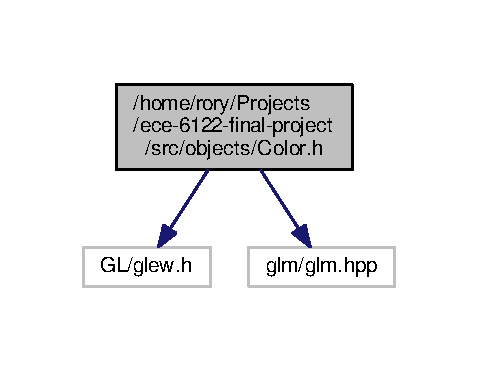
\includegraphics[width=230pt]{_color_8h__incl}
\end{center}
\end{figure}
This graph shows which files directly or indirectly include this file\+:
\nopagebreak
\begin{figure}[H]
\begin{center}
\leavevmode
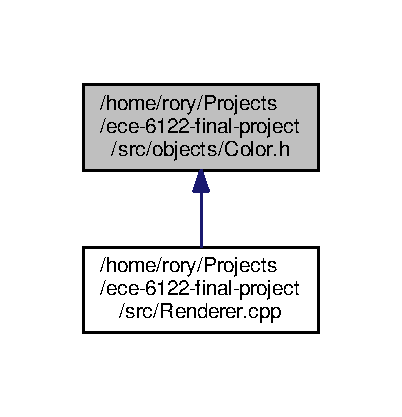
\includegraphics[width=193pt]{_color_8h__dep__incl}
\end{center}
\end{figure}
\subsection*{Classes}
\begin{DoxyCompactItemize}
\item 
struct \hyperlink{struct_color}{Color}
\end{DoxyCompactItemize}

\hypertarget{_face_8h}{}\section{/home/rory/\+Projects/ece-\/6122-\/final-\/project/src/objects/\+Face.h File Reference}
\label{_face_8h}\index{/home/rory/\+Projects/ece-\/6122-\/final-\/project/src/objects/\+Face.\+h@{/home/rory/\+Projects/ece-\/6122-\/final-\/project/src/objects/\+Face.\+h}}
{\ttfamily \#include $<$G\+L/glew.\+h$>$}\newline
{\ttfamily \#include $<$glm/glm.\+hpp$>$}\newline
Include dependency graph for Face.\+h\+:
\nopagebreak
\begin{figure}[H]
\begin{center}
\leavevmode
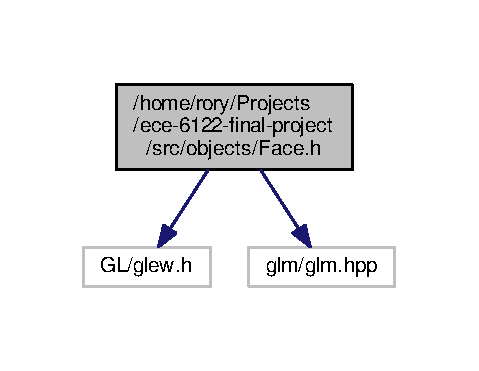
\includegraphics[width=230pt]{_face_8h__incl}
\end{center}
\end{figure}
This graph shows which files directly or indirectly include this file\+:
\nopagebreak
\begin{figure}[H]
\begin{center}
\leavevmode
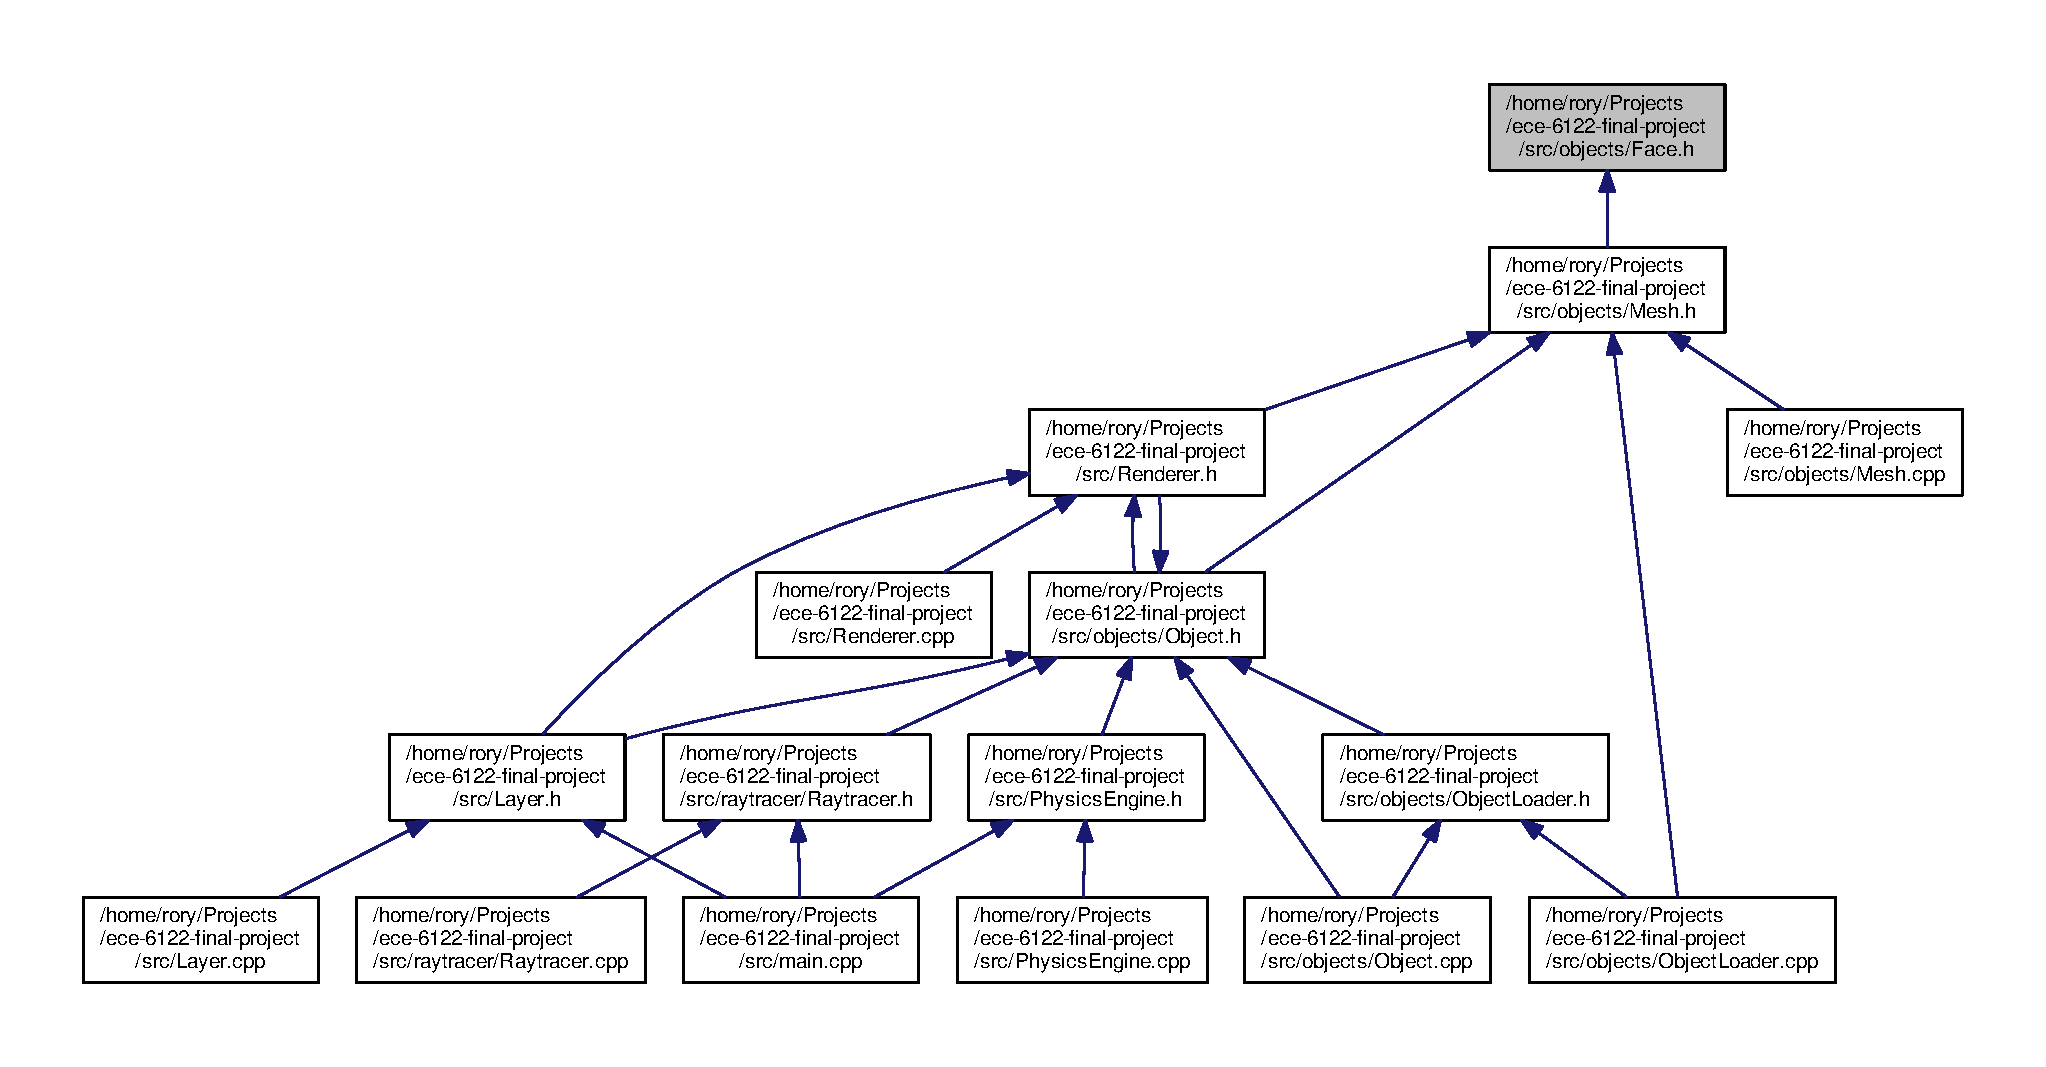
\includegraphics[width=350pt]{_face_8h__dep__incl}
\end{center}
\end{figure}
\subsection*{Classes}
\begin{DoxyCompactItemize}
\item 
struct \hyperlink{struct_face}{Face}
\end{DoxyCompactItemize}

\hypertarget{_material_8cpp}{}\section{/home/rory/\+Projects/ece-\/6122-\/final-\/project/src/objects/\+Material.cpp File Reference}
\label{_material_8cpp}\index{/home/rory/\+Projects/ece-\/6122-\/final-\/project/src/objects/\+Material.\+cpp@{/home/rory/\+Projects/ece-\/6122-\/final-\/project/src/objects/\+Material.\+cpp}}
{\ttfamily \#include \char`\"{}Material.\+h\char`\"{}}\newline
Include dependency graph for Material.\+cpp\+:
\nopagebreak
\begin{figure}[H]
\begin{center}
\leavevmode
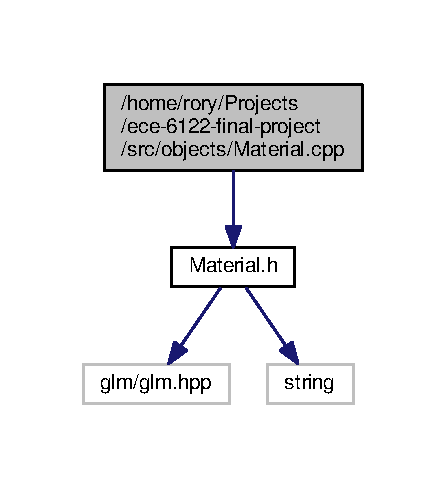
\includegraphics[width=214pt]{_material_8cpp__incl}
\end{center}
\end{figure}
\subsection*{Functions}
\begin{DoxyCompactItemize}
\item 
bool \hyperlink{_material_8cpp_af6a445a8f6268c6b888a45cf4465f642}{operator==} (const \hyperlink{class_material}{Material} \&lhs, const \hyperlink{class_material}{Material} \&rhs)
\end{DoxyCompactItemize}


\subsection{Function Documentation}
\mbox{\Hypertarget{_material_8cpp_af6a445a8f6268c6b888a45cf4465f642}\label{_material_8cpp_af6a445a8f6268c6b888a45cf4465f642}} 
\index{Material.\+cpp@{Material.\+cpp}!operator==@{operator==}}
\index{operator==@{operator==}!Material.\+cpp@{Material.\+cpp}}
\subsubsection{\texorpdfstring{operator==()}{operator==()}}
{\footnotesize\ttfamily bool operator== (\begin{DoxyParamCaption}\item[{const \hyperlink{class_material}{Material} \&}]{lhs,  }\item[{const \hyperlink{class_material}{Material} \&}]{rhs }\end{DoxyParamCaption})}

T\+O\+DO Document 
\begin{DoxyParams}{Parameters}
{\em lhs} & T\+O\+DO Document \\
\hline
{\em rhs} & T\+O\+DO Document \\
\hline
\end{DoxyParams}
\begin{DoxyReturn}{Returns}
T\+O\+DO Document 
\end{DoxyReturn}


Definition at line 17 of file Material.\+cpp.


\hypertarget{_material_8h}{}\section{/home/rory/\+Projects/ece-\/6122-\/final-\/project/src/objects/\+Material.h File Reference}
\label{_material_8h}\index{/home/rory/\+Projects/ece-\/6122-\/final-\/project/src/objects/\+Material.\+h@{/home/rory/\+Projects/ece-\/6122-\/final-\/project/src/objects/\+Material.\+h}}
{\ttfamily \#include $<$glm/glm.\+hpp$>$}\newline
{\ttfamily \#include $<$string$>$}\newline
Include dependency graph for Material.\+h\+:
\nopagebreak
\begin{figure}[H]
\begin{center}
\leavevmode
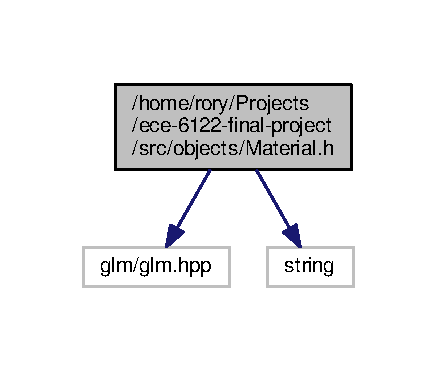
\includegraphics[width=210pt]{_material_8h__incl}
\end{center}
\end{figure}
This graph shows which files directly or indirectly include this file\+:
\nopagebreak
\begin{figure}[H]
\begin{center}
\leavevmode
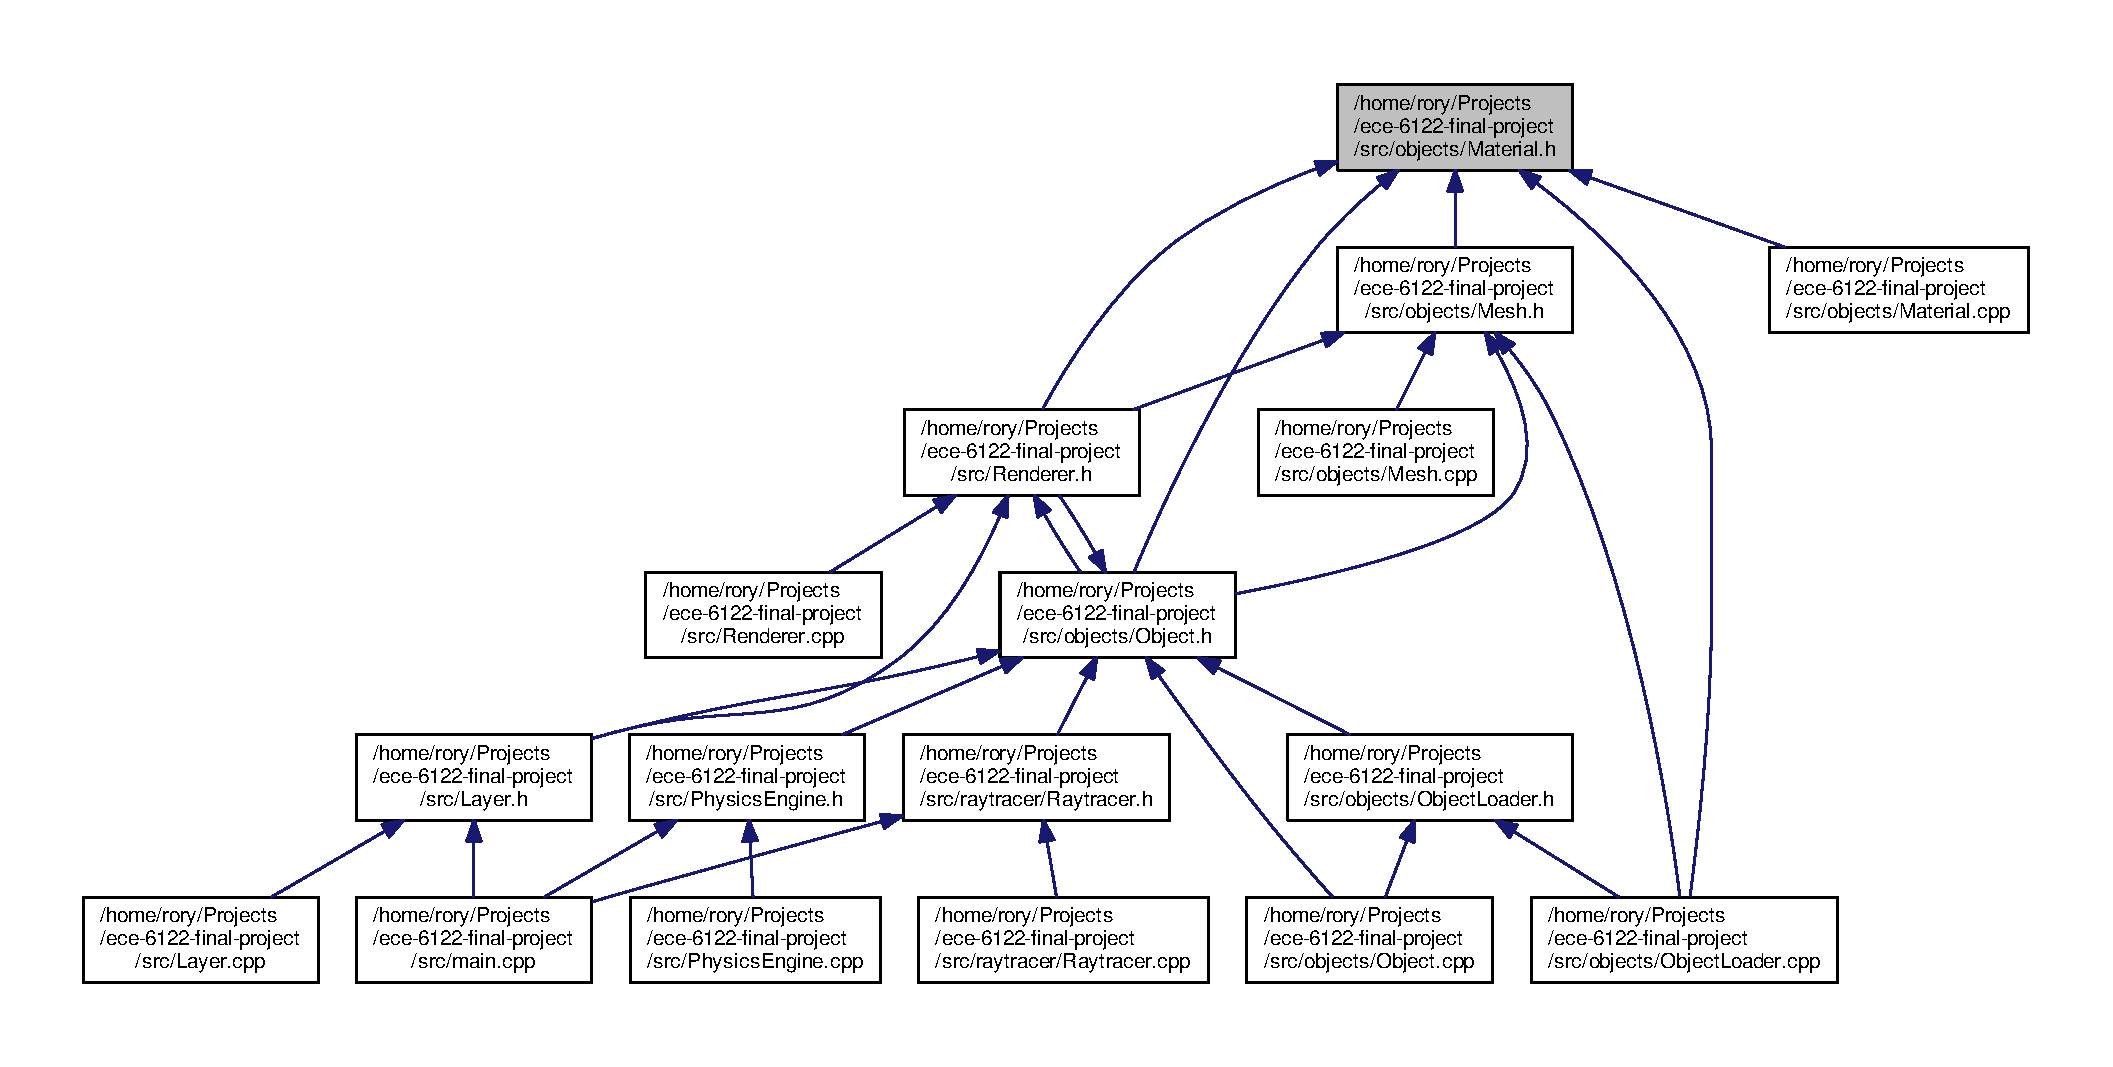
\includegraphics[width=350pt]{_material_8h__dep__incl}
\end{center}
\end{figure}
\subsection*{Classes}
\begin{DoxyCompactItemize}
\item 
class \hyperlink{class_material}{Material}
\end{DoxyCompactItemize}
\subsection*{Functions}
\begin{DoxyCompactItemize}
\item 
bool \hyperlink{_material_8h_af6a445a8f6268c6b888a45cf4465f642}{operator==} (const \hyperlink{class_material}{Material} \&lhs, const \hyperlink{class_material}{Material} \&rhs)
\end{DoxyCompactItemize}


\subsection{Function Documentation}
\mbox{\Hypertarget{_material_8h_af6a445a8f6268c6b888a45cf4465f642}\label{_material_8h_af6a445a8f6268c6b888a45cf4465f642}} 
\index{Material.\+h@{Material.\+h}!operator==@{operator==}}
\index{operator==@{operator==}!Material.\+h@{Material.\+h}}
\subsubsection{\texorpdfstring{operator==()}{operator==()}}
{\footnotesize\ttfamily bool operator== (\begin{DoxyParamCaption}\item[{const \hyperlink{class_material}{Material} \&}]{lhs,  }\item[{const \hyperlink{class_material}{Material} \&}]{rhs }\end{DoxyParamCaption})}

T\+O\+DO Document 
\begin{DoxyParams}{Parameters}
{\em lhs} & T\+O\+DO Document \\
\hline
{\em rhs} & T\+O\+DO Document \\
\hline
\end{DoxyParams}
\begin{DoxyReturn}{Returns}
T\+O\+DO Document 
\end{DoxyReturn}


Definition at line 17 of file Material.\+cpp.


\hypertarget{_mesh_8cpp}{}\section{/home/rory/\+Projects/ece-\/6122-\/final-\/project/src/objects/\+Mesh.cpp File Reference}
\label{_mesh_8cpp}\index{/home/rory/\+Projects/ece-\/6122-\/final-\/project/src/objects/\+Mesh.\+cpp@{/home/rory/\+Projects/ece-\/6122-\/final-\/project/src/objects/\+Mesh.\+cpp}}
{\ttfamily \#include \char`\"{}Mesh.\+h\char`\"{}}\newline
Include dependency graph for Mesh.\+cpp\+:
\nopagebreak
\begin{figure}[H]
\begin{center}
\leavevmode
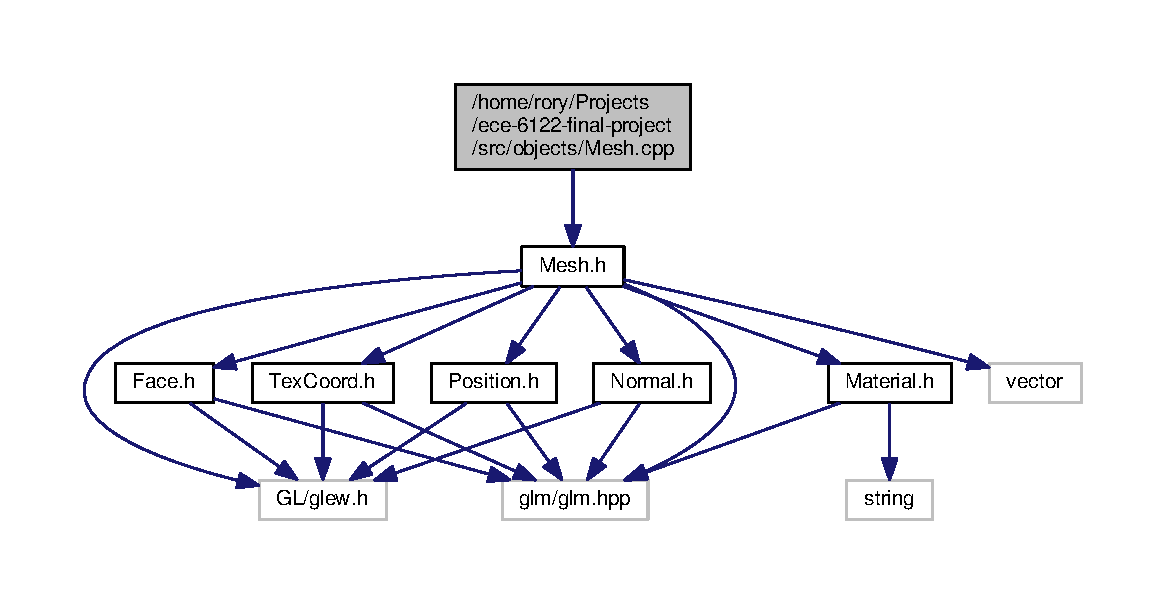
\includegraphics[width=350pt]{_mesh_8cpp__incl}
\end{center}
\end{figure}

\hypertarget{_mesh_8h}{}\section{/home/rory/\+Projects/ece-\/6122-\/final-\/project/src/objects/\+Mesh.h File Reference}
\label{_mesh_8h}\index{/home/rory/\+Projects/ece-\/6122-\/final-\/project/src/objects/\+Mesh.\+h@{/home/rory/\+Projects/ece-\/6122-\/final-\/project/src/objects/\+Mesh.\+h}}
{\ttfamily \#include \char`\"{}Position.\+h\char`\"{}}\newline
{\ttfamily \#include \char`\"{}Normal.\+h\char`\"{}}\newline
{\ttfamily \#include \char`\"{}Face.\+h\char`\"{}}\newline
{\ttfamily \#include \char`\"{}Tex\+Coord.\+h\char`\"{}}\newline
{\ttfamily \#include \char`\"{}Material.\+h\char`\"{}}\newline
{\ttfamily \#include $<$G\+L/glew.\+h$>$}\newline
{\ttfamily \#include $<$glm/glm.\+hpp$>$}\newline
{\ttfamily \#include $<$vector$>$}\newline
Include dependency graph for Mesh.\+h\+:
\nopagebreak
\begin{figure}[H]
\begin{center}
\leavevmode
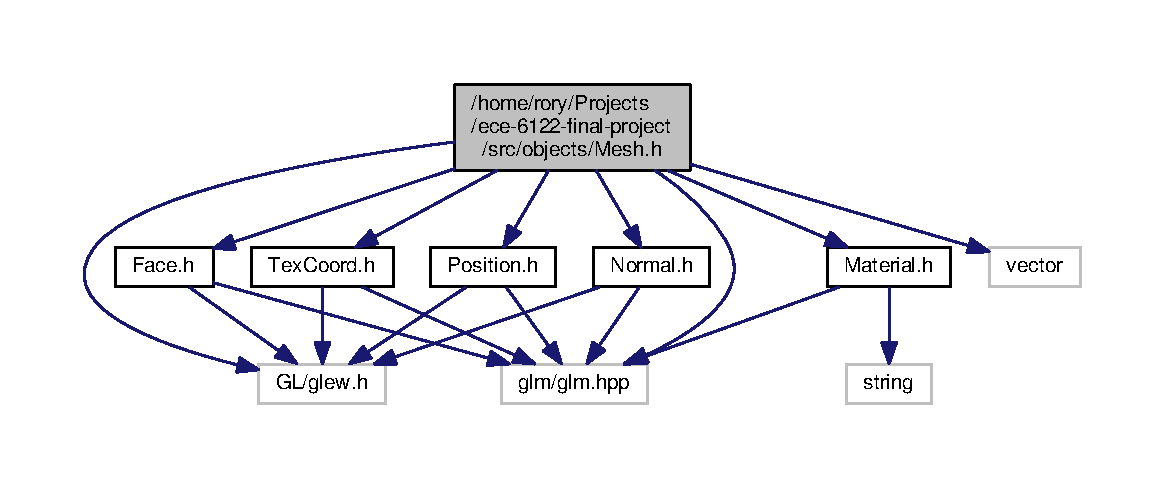
\includegraphics[width=350pt]{_mesh_8h__incl}
\end{center}
\end{figure}
This graph shows which files directly or indirectly include this file\+:
\nopagebreak
\begin{figure}[H]
\begin{center}
\leavevmode
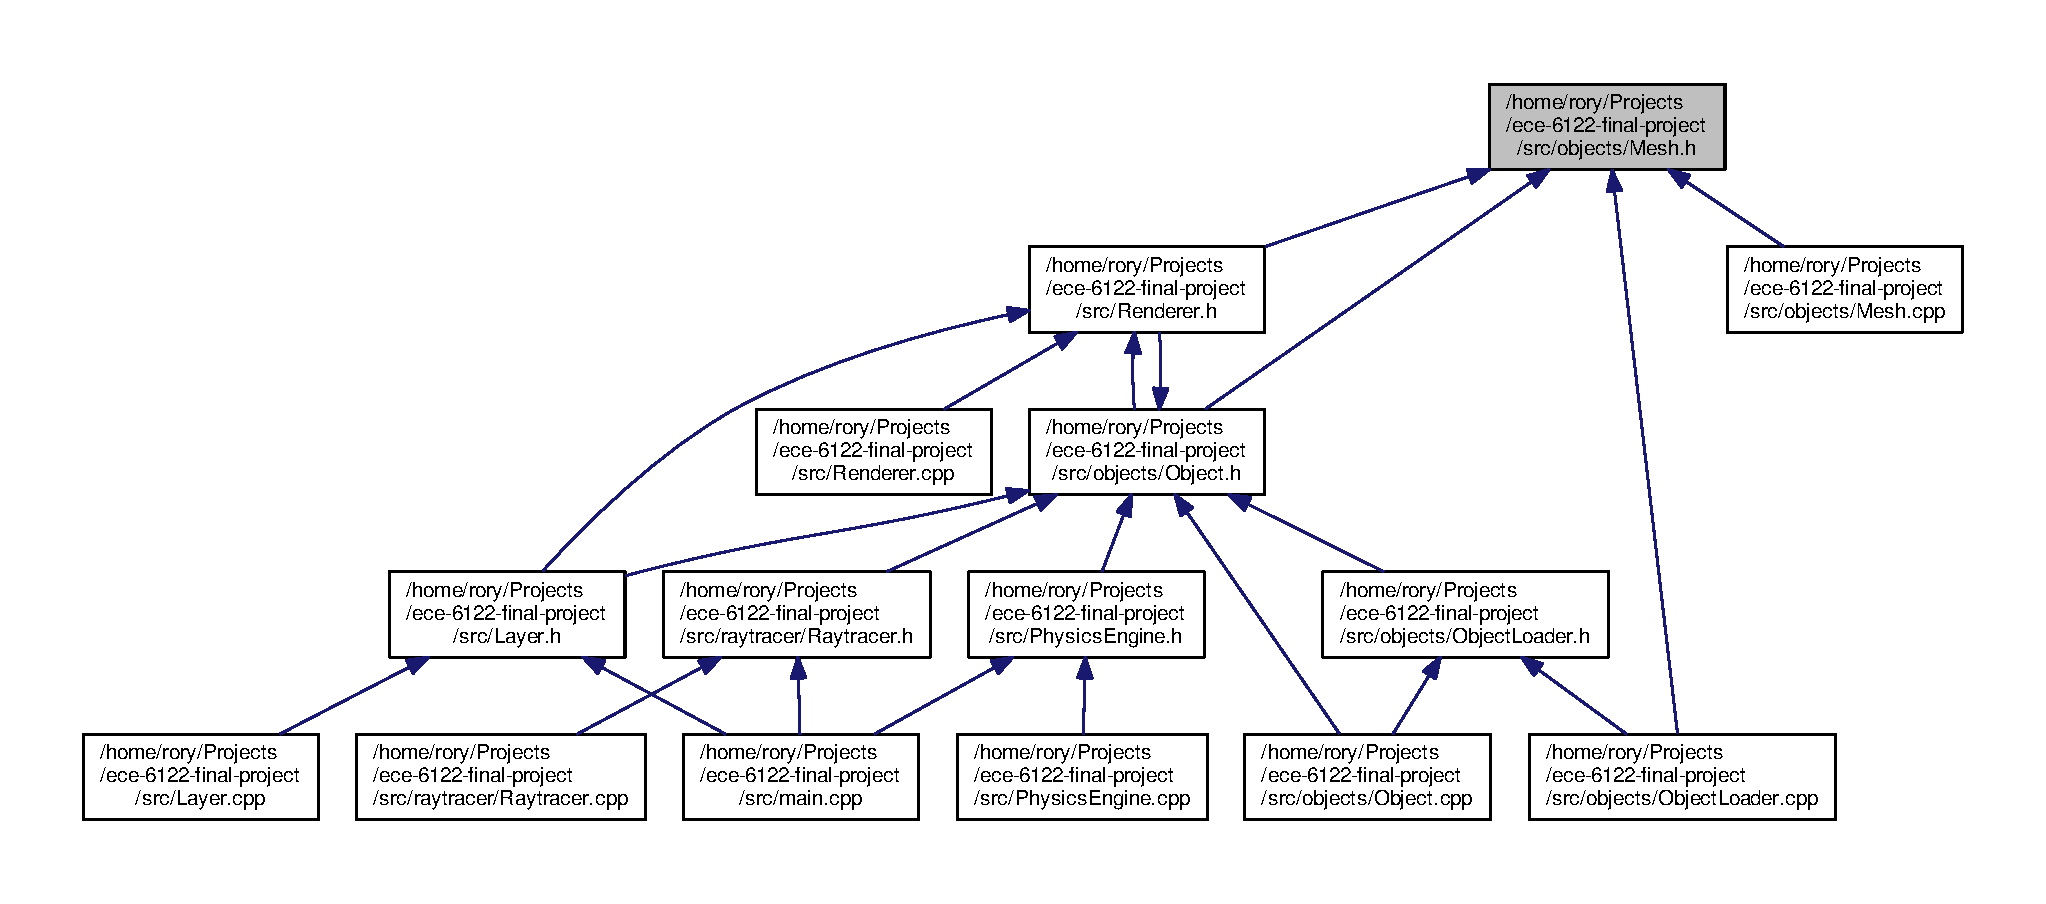
\includegraphics[width=350pt]{_mesh_8h__dep__incl}
\end{center}
\end{figure}
\subsection*{Classes}
\begin{DoxyCompactItemize}
\item 
class \hyperlink{class_mesh}{Mesh}
\end{DoxyCompactItemize}

\hypertarget{_normal_8h}{}\section{/home/rory/\+Projects/ece-\/6122-\/final-\/project/src/objects/\+Normal.h File Reference}
\label{_normal_8h}\index{/home/rory/\+Projects/ece-\/6122-\/final-\/project/src/objects/\+Normal.\+h@{/home/rory/\+Projects/ece-\/6122-\/final-\/project/src/objects/\+Normal.\+h}}
{\ttfamily \#include $<$G\+L/glew.\+h$>$}\newline
{\ttfamily \#include $<$glm/glm.\+hpp$>$}\newline
Include dependency graph for Normal.\+h\+:
\nopagebreak
\begin{figure}[H]
\begin{center}
\leavevmode
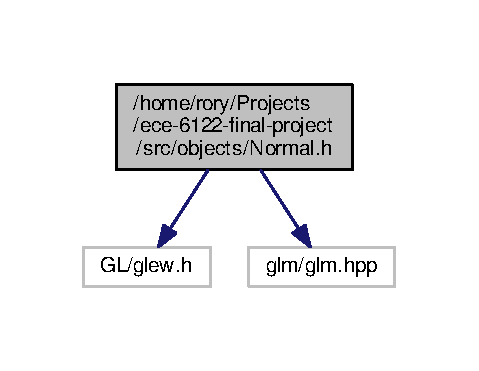
\includegraphics[width=230pt]{_normal_8h__incl}
\end{center}
\end{figure}
This graph shows which files directly or indirectly include this file\+:
\nopagebreak
\begin{figure}[H]
\begin{center}
\leavevmode
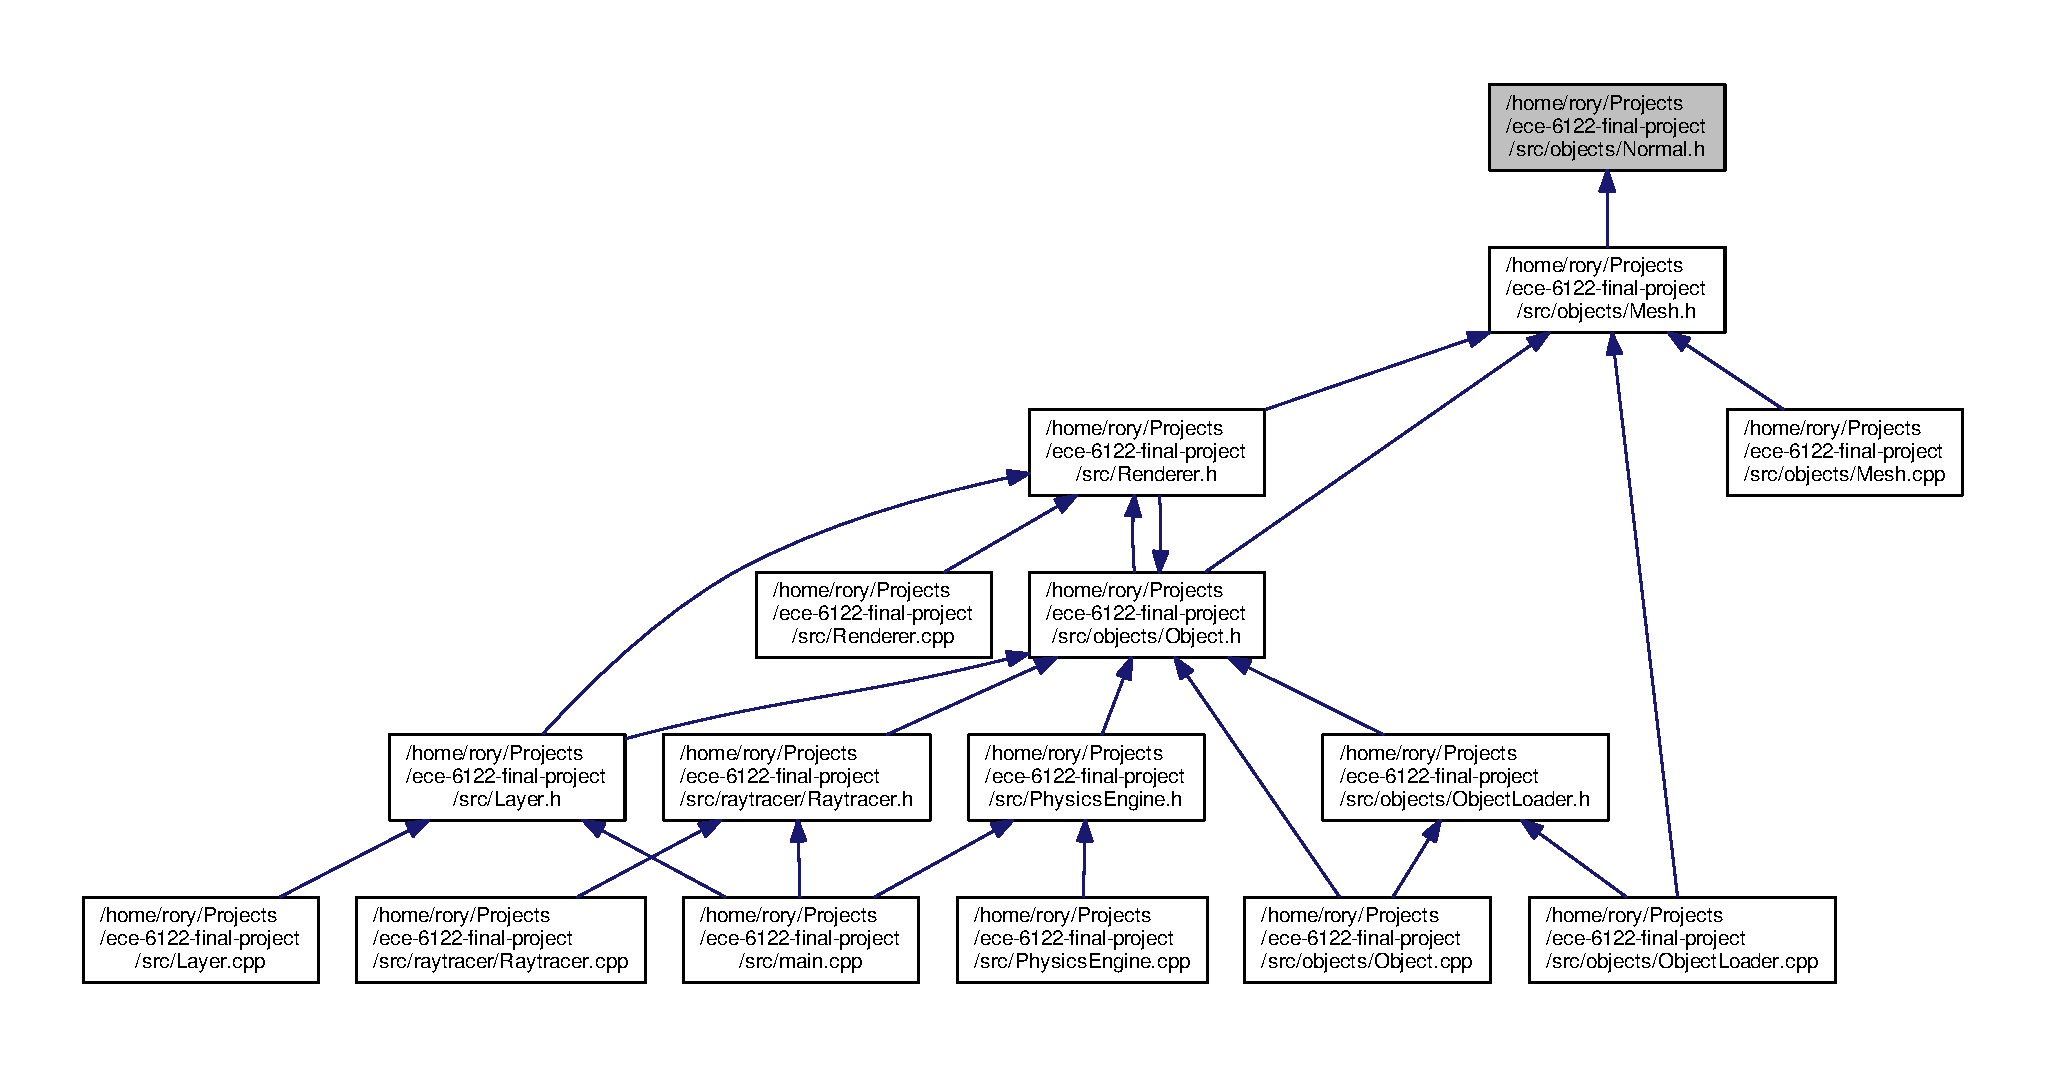
\includegraphics[width=350pt]{_normal_8h__dep__incl}
\end{center}
\end{figure}
\subsection*{Classes}
\begin{DoxyCompactItemize}
\item 
struct \hyperlink{struct_normal}{Normal}
\end{DoxyCompactItemize}

\hypertarget{_object_8cpp}{}\section{/home/rory/\+Projects/ece-\/6122-\/final-\/project/src/objects/\+Object.cpp File Reference}
\label{_object_8cpp}\index{/home/rory/\+Projects/ece-\/6122-\/final-\/project/src/objects/\+Object.\+cpp@{/home/rory/\+Projects/ece-\/6122-\/final-\/project/src/objects/\+Object.\+cpp}}
{\ttfamily \#include \char`\"{}Object.\+h\char`\"{}}\newline
{\ttfamily \#include \char`\"{}Object\+Loader.\+h\char`\"{}}\newline
Include dependency graph for Object.\+cpp\+:
\nopagebreak
\begin{figure}[H]
\begin{center}
\leavevmode
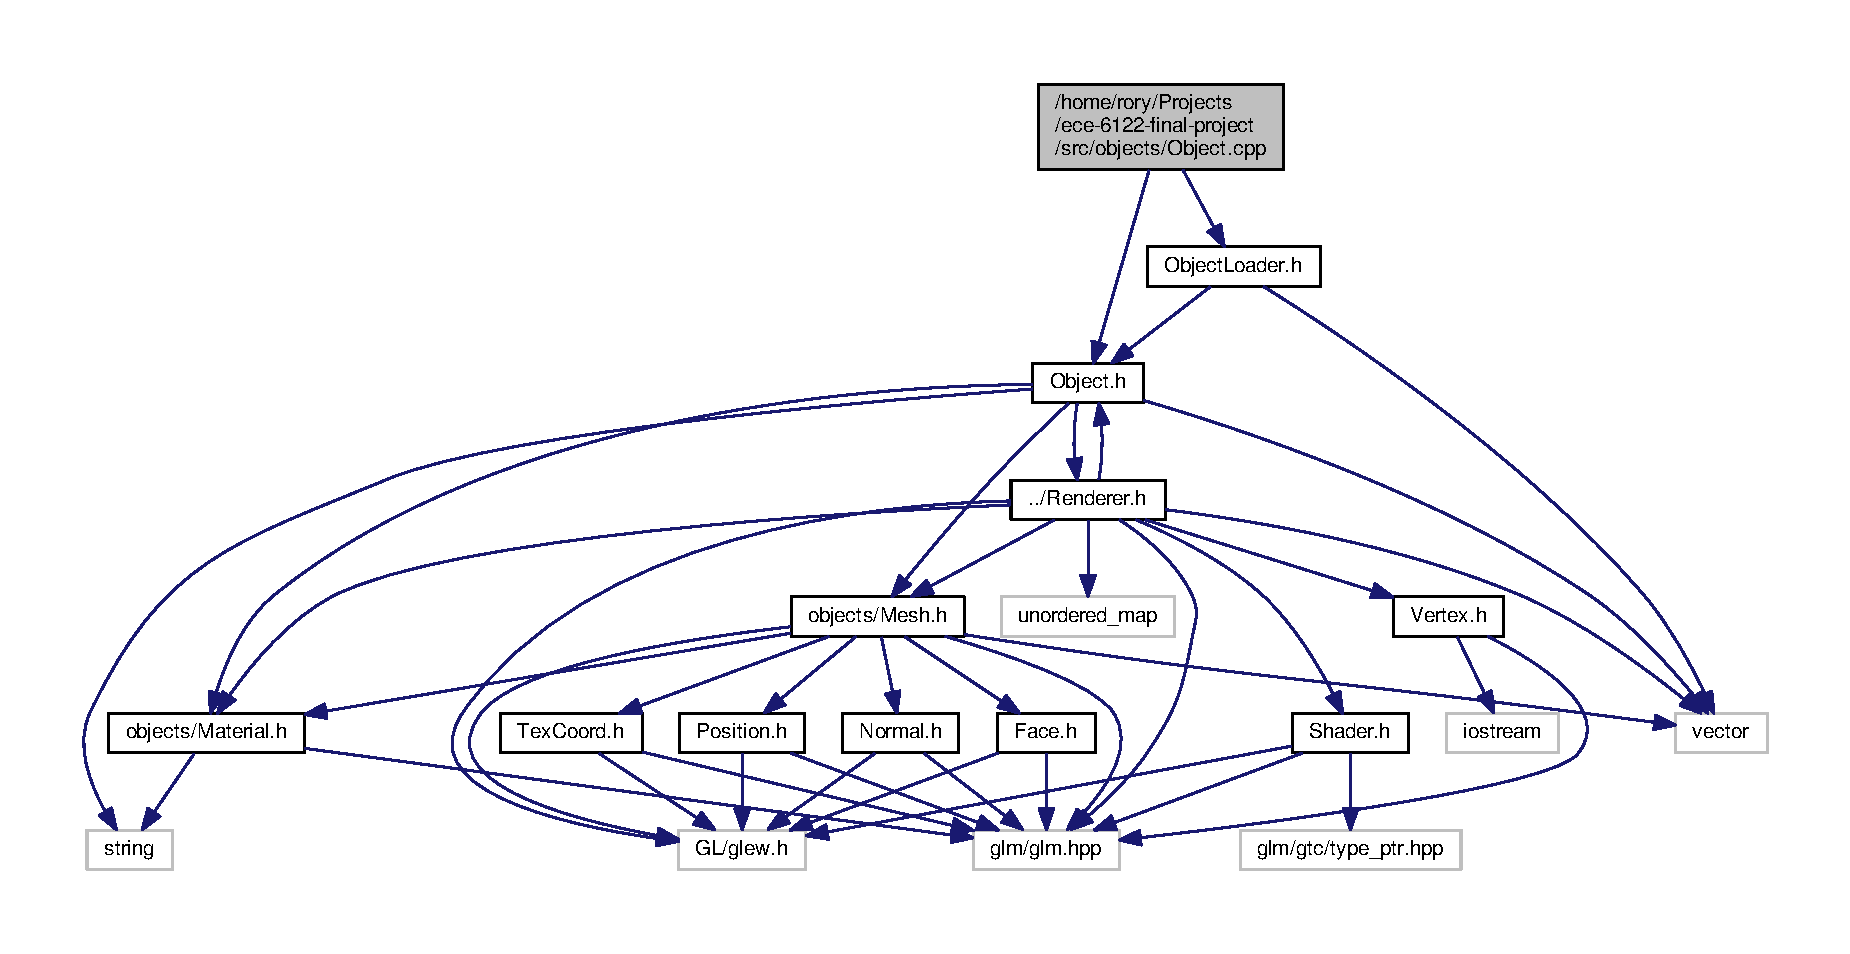
\includegraphics[width=350pt]{_object_8cpp__incl}
\end{center}
\end{figure}

\hypertarget{_object_8h}{}\section{/home/rory/\+Projects/ece-\/6122-\/final-\/project/src/objects/\+Object.h File Reference}
\label{_object_8h}\index{/home/rory/\+Projects/ece-\/6122-\/final-\/project/src/objects/\+Object.\+h@{/home/rory/\+Projects/ece-\/6122-\/final-\/project/src/objects/\+Object.\+h}}
{\ttfamily \#include \char`\"{}../\+Renderer.\+h\char`\"{}}\newline
{\ttfamily \#include \char`\"{}Mesh.\+h\char`\"{}}\newline
{\ttfamily \#include \char`\"{}Material.\+h\char`\"{}}\newline
{\ttfamily \#include $<$vector$>$}\newline
{\ttfamily \#include $<$string$>$}\newline
Include dependency graph for Object.\+h\+:
\nopagebreak
\begin{figure}[H]
\begin{center}
\leavevmode
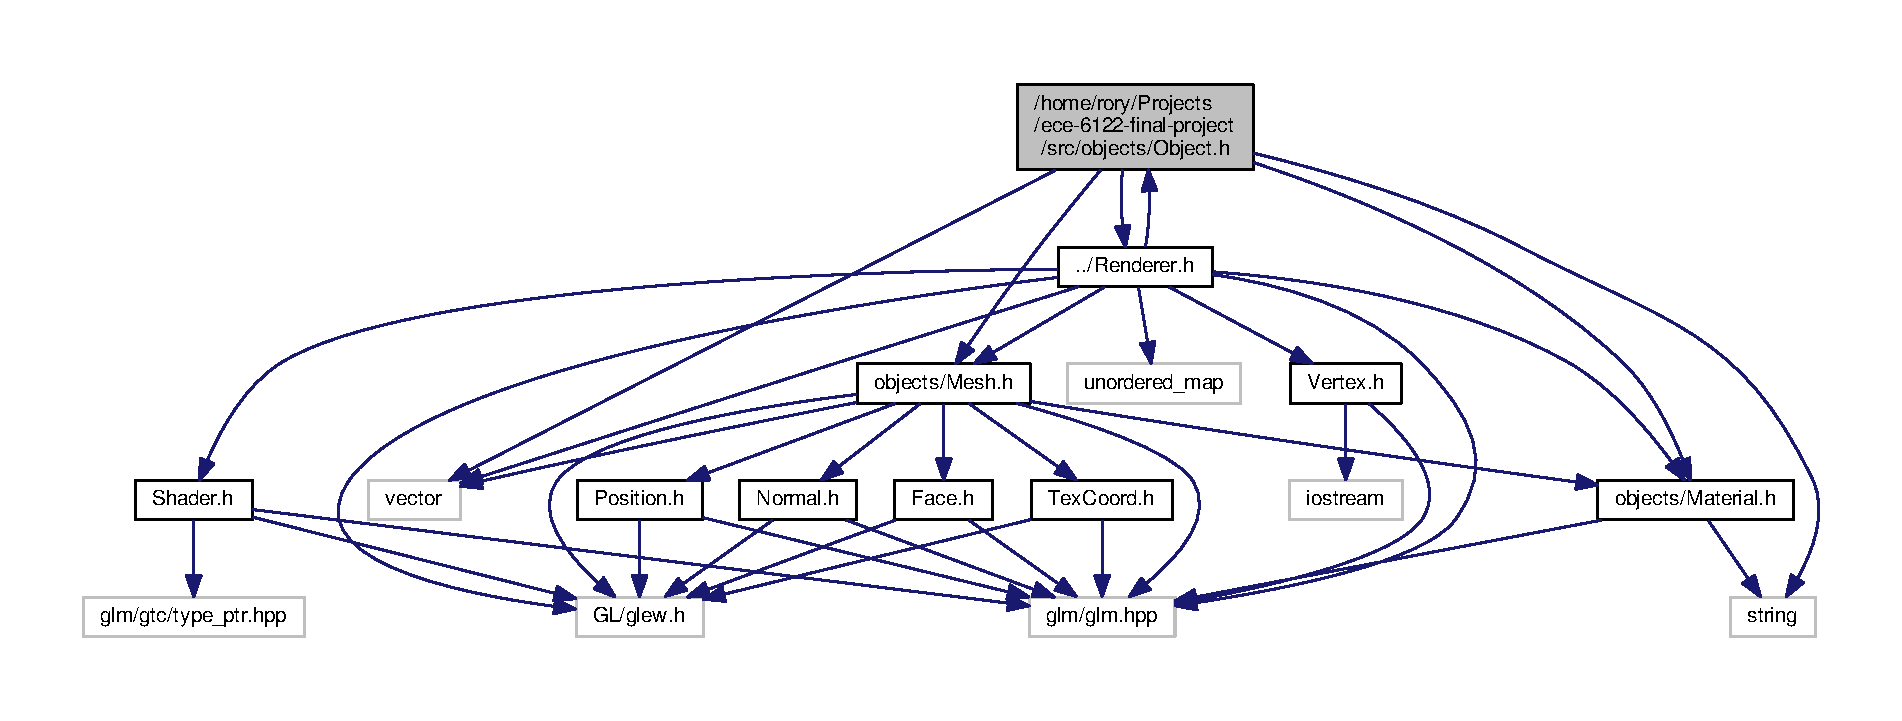
\includegraphics[width=350pt]{_object_8h__incl}
\end{center}
\end{figure}
This graph shows which files directly or indirectly include this file\+:
\nopagebreak
\begin{figure}[H]
\begin{center}
\leavevmode
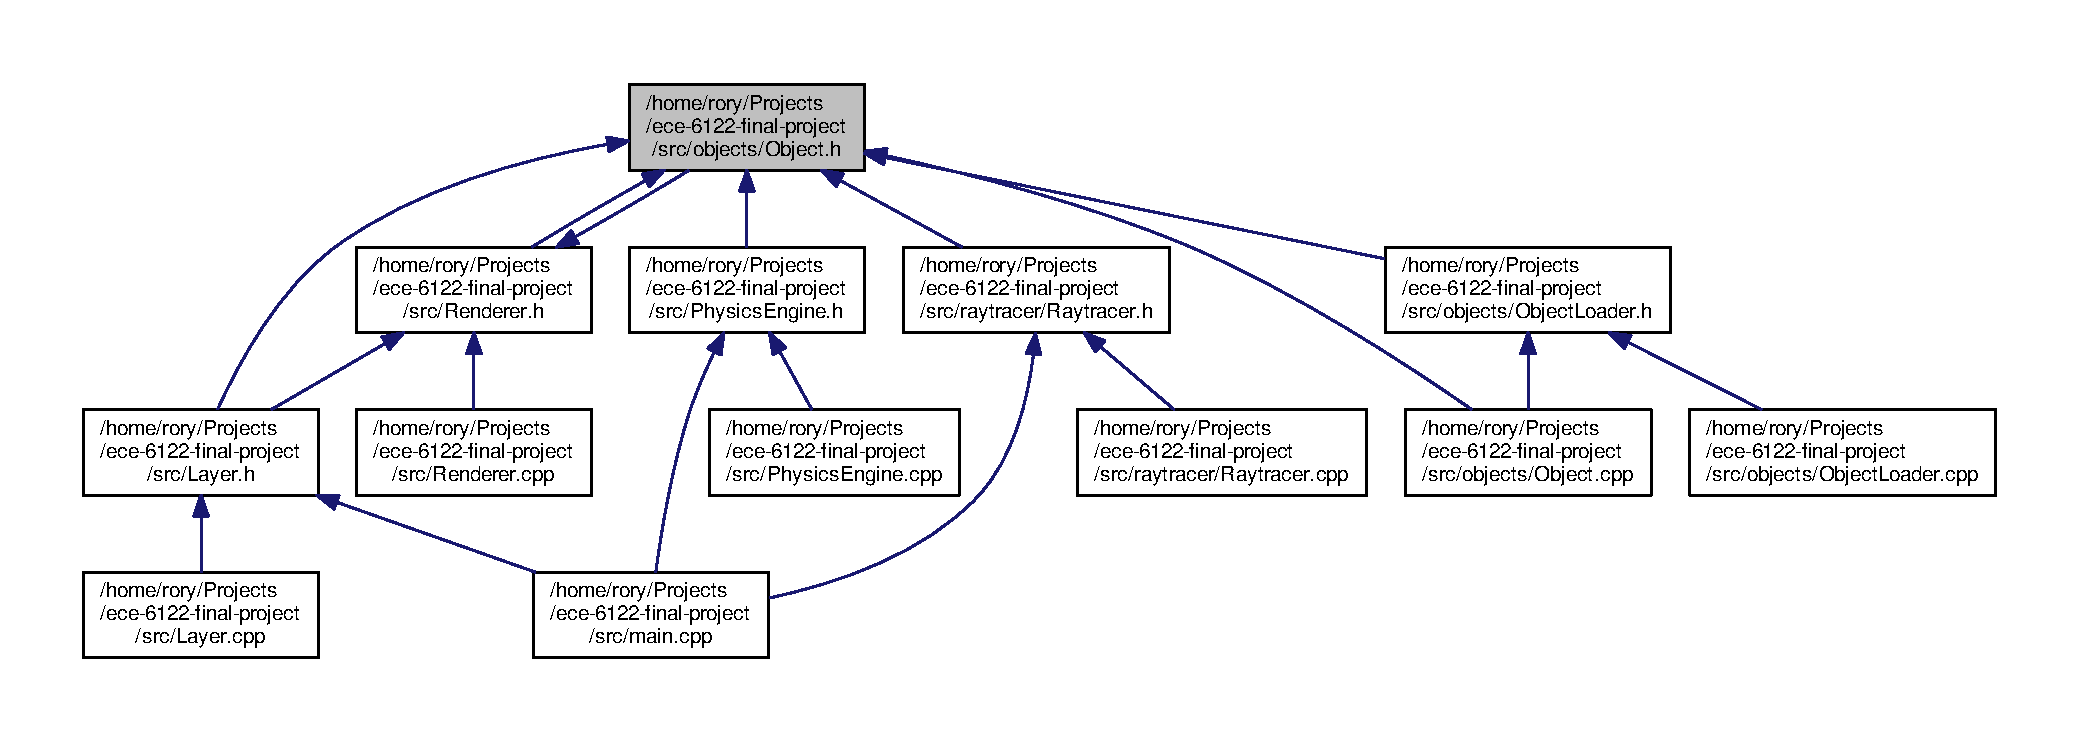
\includegraphics[width=350pt]{_object_8h__dep__incl}
\end{center}
\end{figure}
\subsection*{Classes}
\begin{DoxyCompactItemize}
\item 
class \hyperlink{class_object}{Object}
\end{DoxyCompactItemize}

\hypertarget{_object_loader_8cpp}{}\section{/home/rory/\+Projects/ece-\/6122-\/final-\/project/src/objects/\+Object\+Loader.cpp File Reference}
\label{_object_loader_8cpp}\index{/home/rory/\+Projects/ece-\/6122-\/final-\/project/src/objects/\+Object\+Loader.\+cpp@{/home/rory/\+Projects/ece-\/6122-\/final-\/project/src/objects/\+Object\+Loader.\+cpp}}
{\ttfamily \#include \char`\"{}Object\+Loader.\+h\char`\"{}}\newline
{\ttfamily \#include \char`\"{}Mesh.\+h\char`\"{}}\newline
{\ttfamily \#include \char`\"{}Material.\+h\char`\"{}}\newline
{\ttfamily \#include $<$assimp/\+Importer.\+hpp$>$}\newline
{\ttfamily \#include $<$assimp/postprocess.\+h$>$}\newline
{\ttfamily \#include $<$assimp/scene.\+h$>$}\newline
{\ttfamily \#include $<$iostream$>$}\newline
{\ttfamily \#include $<$fstream$>$}\newline
{\ttfamily \#include $<$unordered\+\_\+map$>$}\newline
Include dependency graph for Object\+Loader.\+cpp\+:
\nopagebreak
\begin{figure}[H]
\begin{center}
\leavevmode
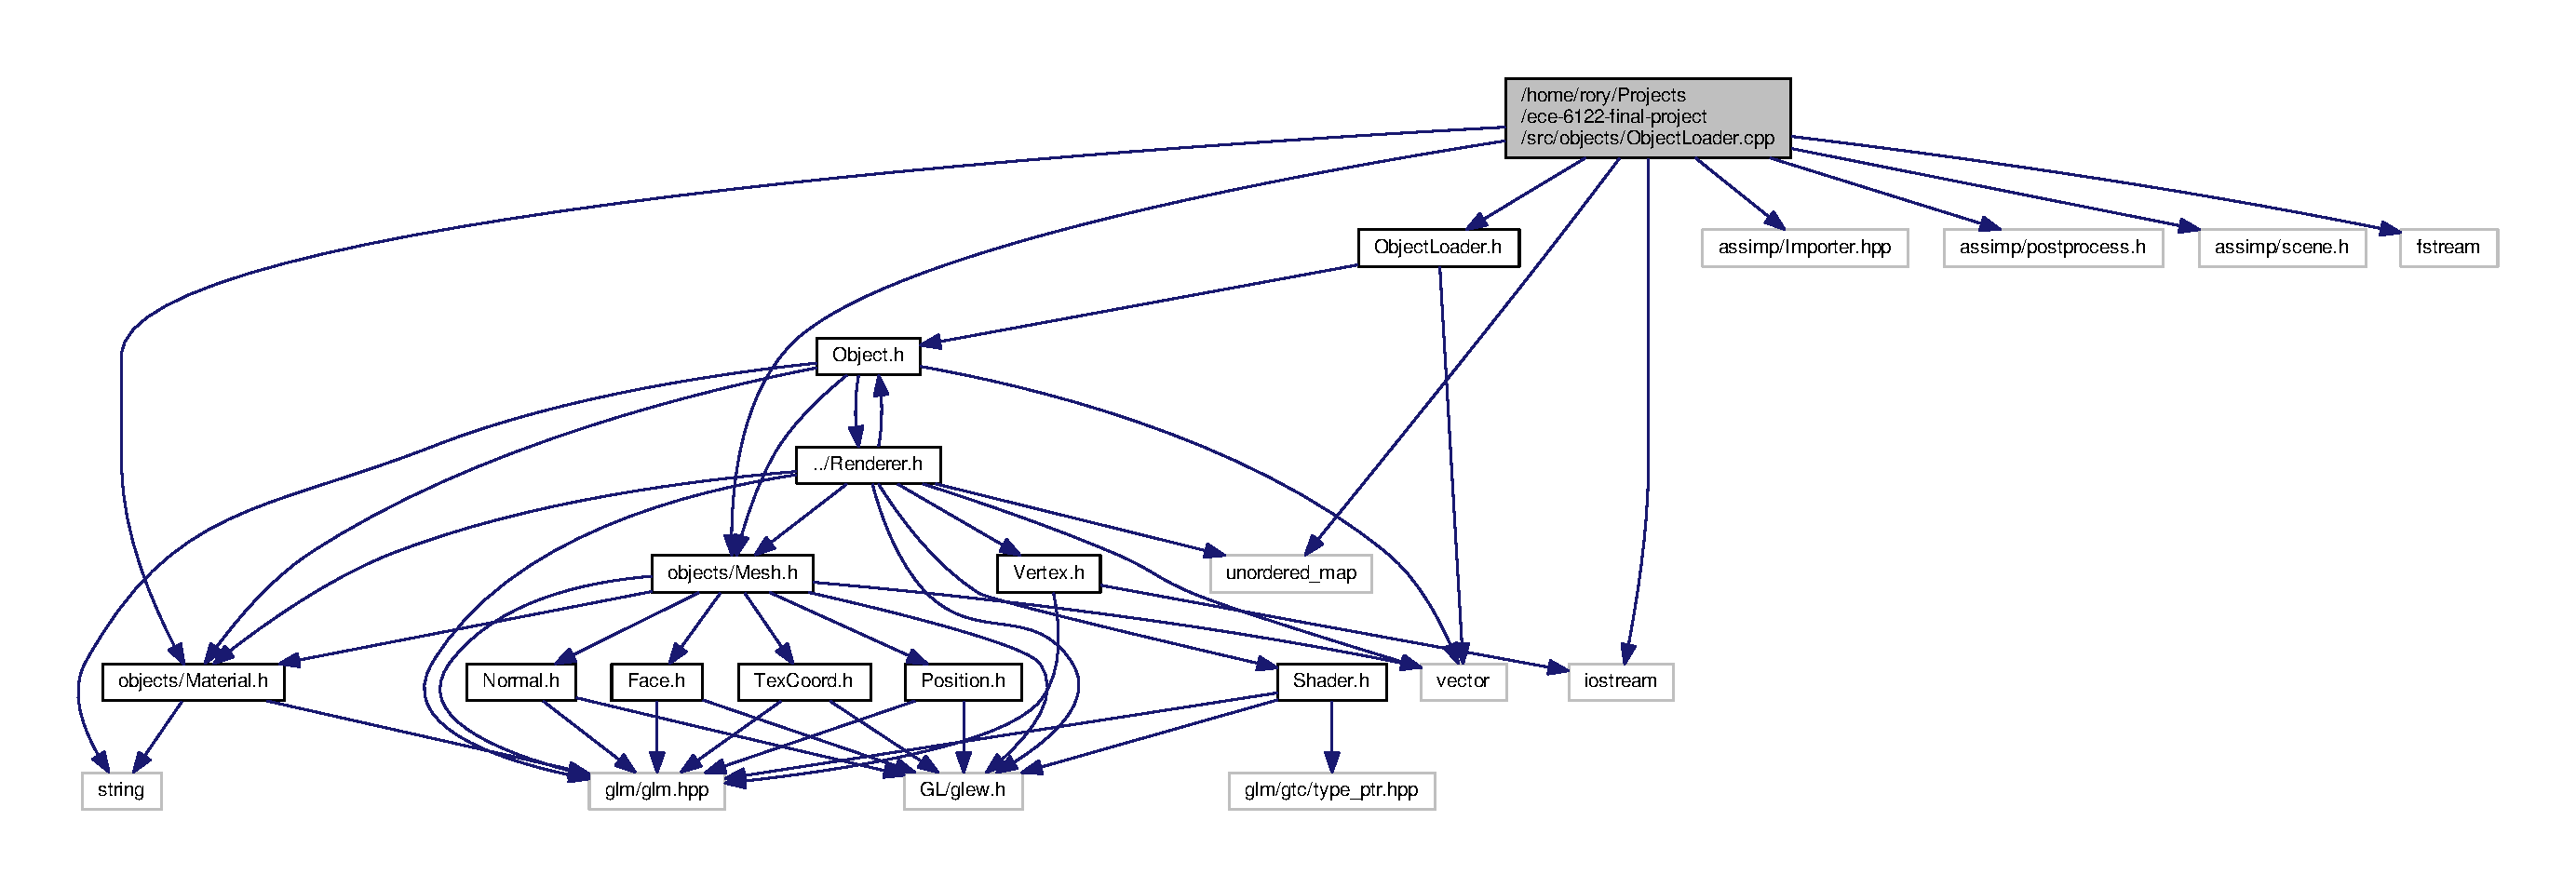
\includegraphics[width=350pt]{_object_loader_8cpp__incl}
\end{center}
\end{figure}
\subsection*{Functions}
\begin{DoxyCompactItemize}
\item 
void \hyperlink{_object_loader_8cpp_a2d2da26d9aa37424cc2837ce3eb3ee96}{create\+Meshes\+From\+Ai\+Scene} (const ai\+Scene $\ast$scene, \hyperlink{class_object}{Object} $\ast$object)
\item 
void \hyperlink{_object_loader_8cpp_a26dbd3b0aee54e7eec20e7d9695c169a}{create\+Materials\+From\+Ai\+Scene} (const ai\+Scene $\ast$scene, \hyperlink{class_object}{Object} $\ast$object)
\item 
void \hyperlink{_object_loader_8cpp_ab750877f926b1943508db516d72eba47}{print\+Ai\+Scene\+Info} (const ai\+Scene $\ast$scene)
\item 
void \hyperlink{_object_loader_8cpp_a1d57b7e7c673c74a54574ab2237eaf0e}{print\+Vector3D} (string name, ai\+Vector3D vector)
\item 
void \hyperlink{_object_loader_8cpp_a284eaf64f035f96f14d923256f0dca79}{print\+Color3D} (string name, ai\+Color3D color)
\item 
void \hyperlink{_object_loader_8cpp_a2f1e5dd30e5903db9ee29e2d4efdd933}{indent} (unsigned int layer)
\item 
void \hyperlink{_object_loader_8cpp_ac886656c40740bc679804ee79b73a609}{print\+Matrix4x4} (ai\+Matrix4x4 matrix, unsigned int layer=0)
\item 
void \hyperlink{_object_loader_8cpp_a2d827d20b346b6b38aa4623f4fd3f633}{print\+Node\+Tree} (const ai\+Node $\ast$node, unsigned int layer)
\end{DoxyCompactItemize}


\subsection{Function Documentation}
\mbox{\Hypertarget{_object_loader_8cpp_a26dbd3b0aee54e7eec20e7d9695c169a}\label{_object_loader_8cpp_a26dbd3b0aee54e7eec20e7d9695c169a}} 
\index{Object\+Loader.\+cpp@{Object\+Loader.\+cpp}!create\+Materials\+From\+Ai\+Scene@{create\+Materials\+From\+Ai\+Scene}}
\index{create\+Materials\+From\+Ai\+Scene@{create\+Materials\+From\+Ai\+Scene}!Object\+Loader.\+cpp@{Object\+Loader.\+cpp}}
\subsubsection{\texorpdfstring{create\+Materials\+From\+Ai\+Scene()}{createMaterialsFromAiScene()}}
{\footnotesize\ttfamily void create\+Materials\+From\+Ai\+Scene (\begin{DoxyParamCaption}\item[{const ai\+Scene $\ast$}]{scene,  }\item[{\hyperlink{class_object}{Object} $\ast$}]{object }\end{DoxyParamCaption})}

Create material objects from an ai\+Scene 
\begin{DoxyParams}{Parameters}
{\em scene} & The ai\+Scene containing the materials \\
\hline
\end{DoxyParams}


Definition at line 170 of file Object\+Loader.\+cpp.

\mbox{\Hypertarget{_object_loader_8cpp_a2d2da26d9aa37424cc2837ce3eb3ee96}\label{_object_loader_8cpp_a2d2da26d9aa37424cc2837ce3eb3ee96}} 
\index{Object\+Loader.\+cpp@{Object\+Loader.\+cpp}!create\+Meshes\+From\+Ai\+Scene@{create\+Meshes\+From\+Ai\+Scene}}
\index{create\+Meshes\+From\+Ai\+Scene@{create\+Meshes\+From\+Ai\+Scene}!Object\+Loader.\+cpp@{Object\+Loader.\+cpp}}
\subsubsection{\texorpdfstring{create\+Meshes\+From\+Ai\+Scene()}{createMeshesFromAiScene()}}
{\footnotesize\ttfamily void create\+Meshes\+From\+Ai\+Scene (\begin{DoxyParamCaption}\item[{const ai\+Scene $\ast$}]{scene,  }\item[{\hyperlink{class_object}{Object} $\ast$}]{object }\end{DoxyParamCaption})}

T\+O\+DO 
\begin{DoxyParams}{Parameters}
{\em scene} & T\+O\+DO \\
\hline
\end{DoxyParams}
\begin{DoxyReturn}{Returns}
T\+O\+DO 
\end{DoxyReturn}


Definition at line 71 of file Object\+Loader.\+cpp.

\mbox{\Hypertarget{_object_loader_8cpp_a2f1e5dd30e5903db9ee29e2d4efdd933}\label{_object_loader_8cpp_a2f1e5dd30e5903db9ee29e2d4efdd933}} 
\index{Object\+Loader.\+cpp@{Object\+Loader.\+cpp}!indent@{indent}}
\index{indent@{indent}!Object\+Loader.\+cpp@{Object\+Loader.\+cpp}}
\subsubsection{\texorpdfstring{indent()}{indent()}}
{\footnotesize\ttfamily void indent (\begin{DoxyParamCaption}\item[{unsigned int}]{layer }\end{DoxyParamCaption})}

T\+O\+DO 
\begin{DoxyParams}{Parameters}
{\em layer} & T\+O\+DO \\
\hline
\end{DoxyParams}


Definition at line 312 of file Object\+Loader.\+cpp.

\mbox{\Hypertarget{_object_loader_8cpp_ab750877f926b1943508db516d72eba47}\label{_object_loader_8cpp_ab750877f926b1943508db516d72eba47}} 
\index{Object\+Loader.\+cpp@{Object\+Loader.\+cpp}!print\+Ai\+Scene\+Info@{print\+Ai\+Scene\+Info}}
\index{print\+Ai\+Scene\+Info@{print\+Ai\+Scene\+Info}!Object\+Loader.\+cpp@{Object\+Loader.\+cpp}}
\subsubsection{\texorpdfstring{print\+Ai\+Scene\+Info()}{printAiSceneInfo()}}
{\footnotesize\ttfamily void print\+Ai\+Scene\+Info (\begin{DoxyParamCaption}\item[{const ai\+Scene $\ast$}]{scene }\end{DoxyParamCaption})}

T\+O\+DO 
\begin{DoxyParams}{Parameters}
{\em scene} & T\+O\+DO \\
\hline
\end{DoxyParams}


Definition at line 386 of file Object\+Loader.\+cpp.

\mbox{\Hypertarget{_object_loader_8cpp_a284eaf64f035f96f14d923256f0dca79}\label{_object_loader_8cpp_a284eaf64f035f96f14d923256f0dca79}} 
\index{Object\+Loader.\+cpp@{Object\+Loader.\+cpp}!print\+Color3D@{print\+Color3D}}
\index{print\+Color3D@{print\+Color3D}!Object\+Loader.\+cpp@{Object\+Loader.\+cpp}}
\subsubsection{\texorpdfstring{print\+Color3\+D()}{printColor3D()}}
{\footnotesize\ttfamily void print\+Color3D (\begin{DoxyParamCaption}\item[{string}]{name,  }\item[{ai\+Color3D}]{color }\end{DoxyParamCaption})}

T\+O\+DO 
\begin{DoxyParams}{Parameters}
{\em name} & T\+O\+DO \\
\hline
{\em color} & T\+O\+DO \\
\hline
\end{DoxyParams}


Definition at line 301 of file Object\+Loader.\+cpp.

\mbox{\Hypertarget{_object_loader_8cpp_ac886656c40740bc679804ee79b73a609}\label{_object_loader_8cpp_ac886656c40740bc679804ee79b73a609}} 
\index{Object\+Loader.\+cpp@{Object\+Loader.\+cpp}!print\+Matrix4x4@{print\+Matrix4x4}}
\index{print\+Matrix4x4@{print\+Matrix4x4}!Object\+Loader.\+cpp@{Object\+Loader.\+cpp}}
\subsubsection{\texorpdfstring{print\+Matrix4x4()}{printMatrix4x4()}}
{\footnotesize\ttfamily void print\+Matrix4x4 (\begin{DoxyParamCaption}\item[{ai\+Matrix4x4}]{matrix,  }\item[{unsigned int}]{layer = {\ttfamily 0} }\end{DoxyParamCaption})}

T\+O\+DO 
\begin{DoxyParams}{Parameters}
{\em matrix} & T\+O\+DO \\
\hline
{\em layer} & T\+O\+DO \\
\hline
\end{DoxyParams}


Definition at line 325 of file Object\+Loader.\+cpp.

\mbox{\Hypertarget{_object_loader_8cpp_a2d827d20b346b6b38aa4623f4fd3f633}\label{_object_loader_8cpp_a2d827d20b346b6b38aa4623f4fd3f633}} 
\index{Object\+Loader.\+cpp@{Object\+Loader.\+cpp}!print\+Node\+Tree@{print\+Node\+Tree}}
\index{print\+Node\+Tree@{print\+Node\+Tree}!Object\+Loader.\+cpp@{Object\+Loader.\+cpp}}
\subsubsection{\texorpdfstring{print\+Node\+Tree()}{printNodeTree()}}
{\footnotesize\ttfamily void print\+Node\+Tree (\begin{DoxyParamCaption}\item[{const ai\+Node $\ast$}]{node,  }\item[{unsigned int}]{layer }\end{DoxyParamCaption})}

T\+O\+DO 
\begin{DoxyParams}{Parameters}
{\em node} & T\+O\+DO \\
\hline
{\em layer} & T\+O\+DO \\
\hline
\end{DoxyParams}


Definition at line 342 of file Object\+Loader.\+cpp.

\mbox{\Hypertarget{_object_loader_8cpp_a1d57b7e7c673c74a54574ab2237eaf0e}\label{_object_loader_8cpp_a1d57b7e7c673c74a54574ab2237eaf0e}} 
\index{Object\+Loader.\+cpp@{Object\+Loader.\+cpp}!print\+Vector3D@{print\+Vector3D}}
\index{print\+Vector3D@{print\+Vector3D}!Object\+Loader.\+cpp@{Object\+Loader.\+cpp}}
\subsubsection{\texorpdfstring{print\+Vector3\+D()}{printVector3D()}}
{\footnotesize\ttfamily void print\+Vector3D (\begin{DoxyParamCaption}\item[{string}]{name,  }\item[{ai\+Vector3D}]{vector }\end{DoxyParamCaption})}

T\+O\+DO 
\begin{DoxyParams}{Parameters}
{\em name} & T\+O\+DO \\
\hline
{\em vector} & T\+O\+DO \\
\hline
\end{DoxyParams}


Definition at line 289 of file Object\+Loader.\+cpp.


\hypertarget{_object_loader_8h}{}\section{/home/rory/\+Projects/ece-\/6122-\/final-\/project/src/objects/\+Object\+Loader.h File Reference}
\label{_object_loader_8h}\index{/home/rory/\+Projects/ece-\/6122-\/final-\/project/src/objects/\+Object\+Loader.\+h@{/home/rory/\+Projects/ece-\/6122-\/final-\/project/src/objects/\+Object\+Loader.\+h}}
{\ttfamily \#include \char`\"{}Object.\+h\char`\"{}}\newline
{\ttfamily \#include $<$vector$>$}\newline
Include dependency graph for Object\+Loader.\+h\+:
\nopagebreak
\begin{figure}[H]
\begin{center}
\leavevmode
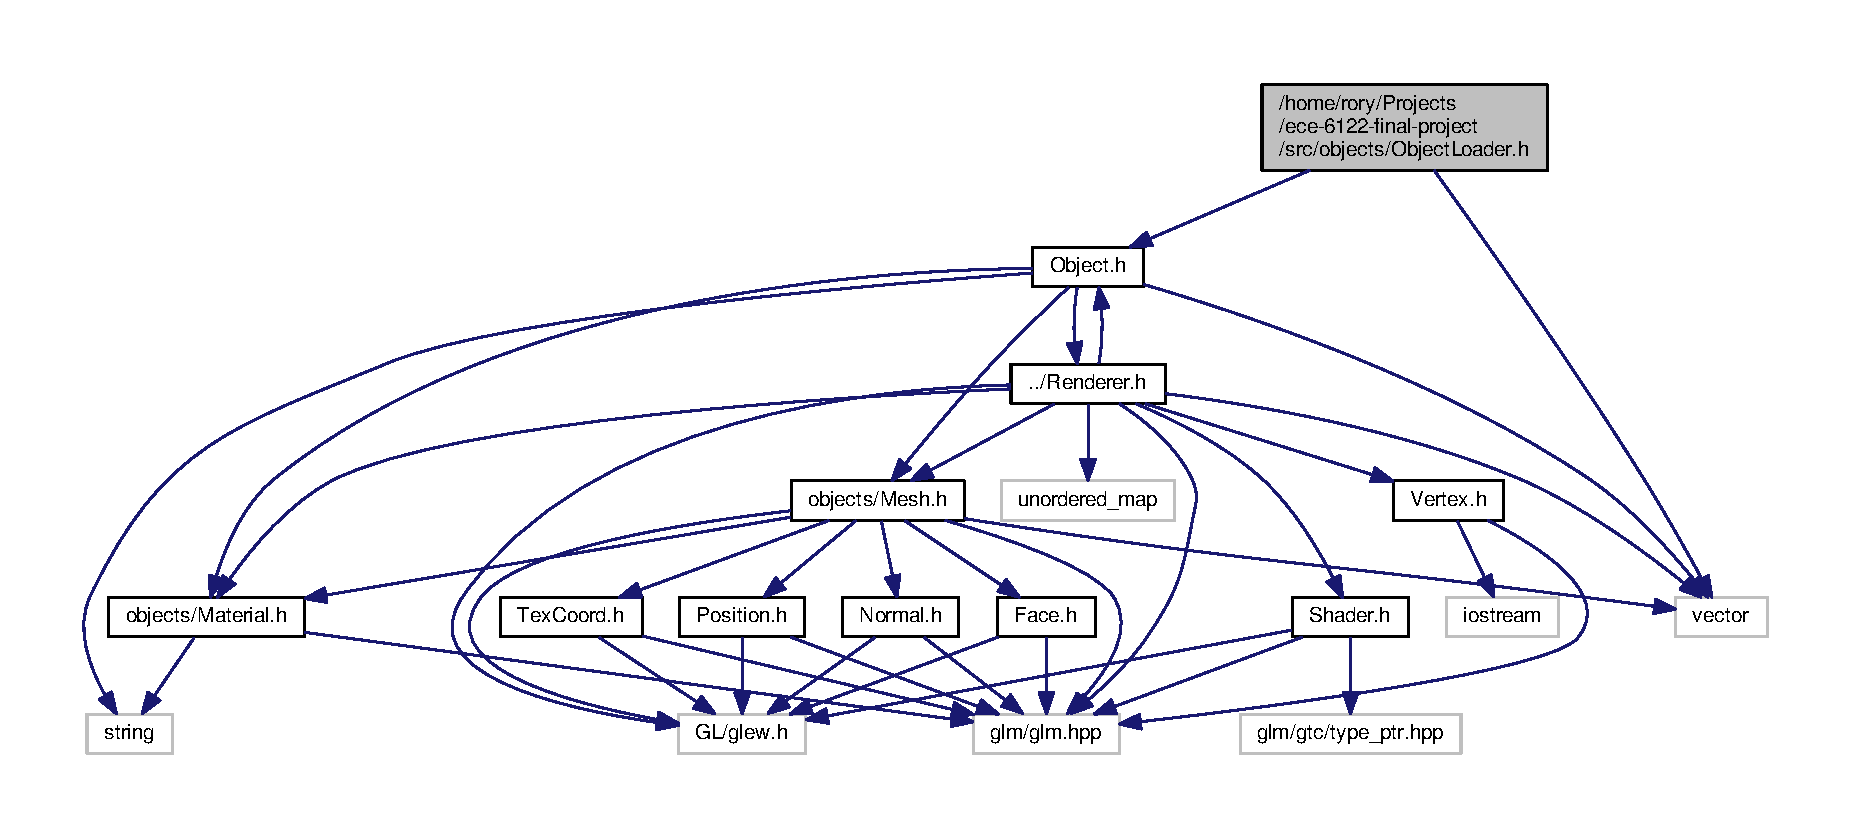
\includegraphics[width=350pt]{_object_loader_8h__incl}
\end{center}
\end{figure}
This graph shows which files directly or indirectly include this file\+:
\nopagebreak
\begin{figure}[H]
\begin{center}
\leavevmode
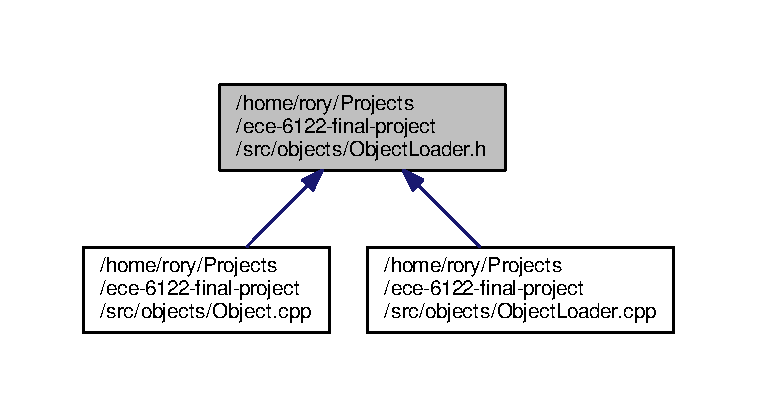
\includegraphics[width=350pt]{_object_loader_8h__dep__incl}
\end{center}
\end{figure}
\subsection*{Classes}
\begin{DoxyCompactItemize}
\item 
class \hyperlink{class_object_loader}{Object\+Loader}
\end{DoxyCompactItemize}

\hypertarget{_position_8h}{}\section{/home/rory/\+Projects/ece-\/6122-\/final-\/project/src/objects/\+Position.h File Reference}
\label{_position_8h}\index{/home/rory/\+Projects/ece-\/6122-\/final-\/project/src/objects/\+Position.\+h@{/home/rory/\+Projects/ece-\/6122-\/final-\/project/src/objects/\+Position.\+h}}
{\ttfamily \#include $<$G\+L/glew.\+h$>$}\newline
{\ttfamily \#include $<$glm/glm.\+hpp$>$}\newline
Include dependency graph for Position.\+h\+:
\nopagebreak
\begin{figure}[H]
\begin{center}
\leavevmode
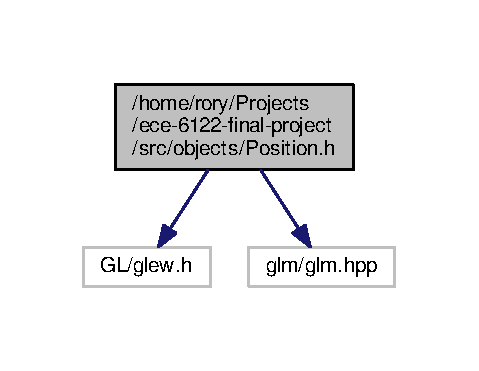
\includegraphics[width=230pt]{_position_8h__incl}
\end{center}
\end{figure}
This graph shows which files directly or indirectly include this file\+:
\nopagebreak
\begin{figure}[H]
\begin{center}
\leavevmode
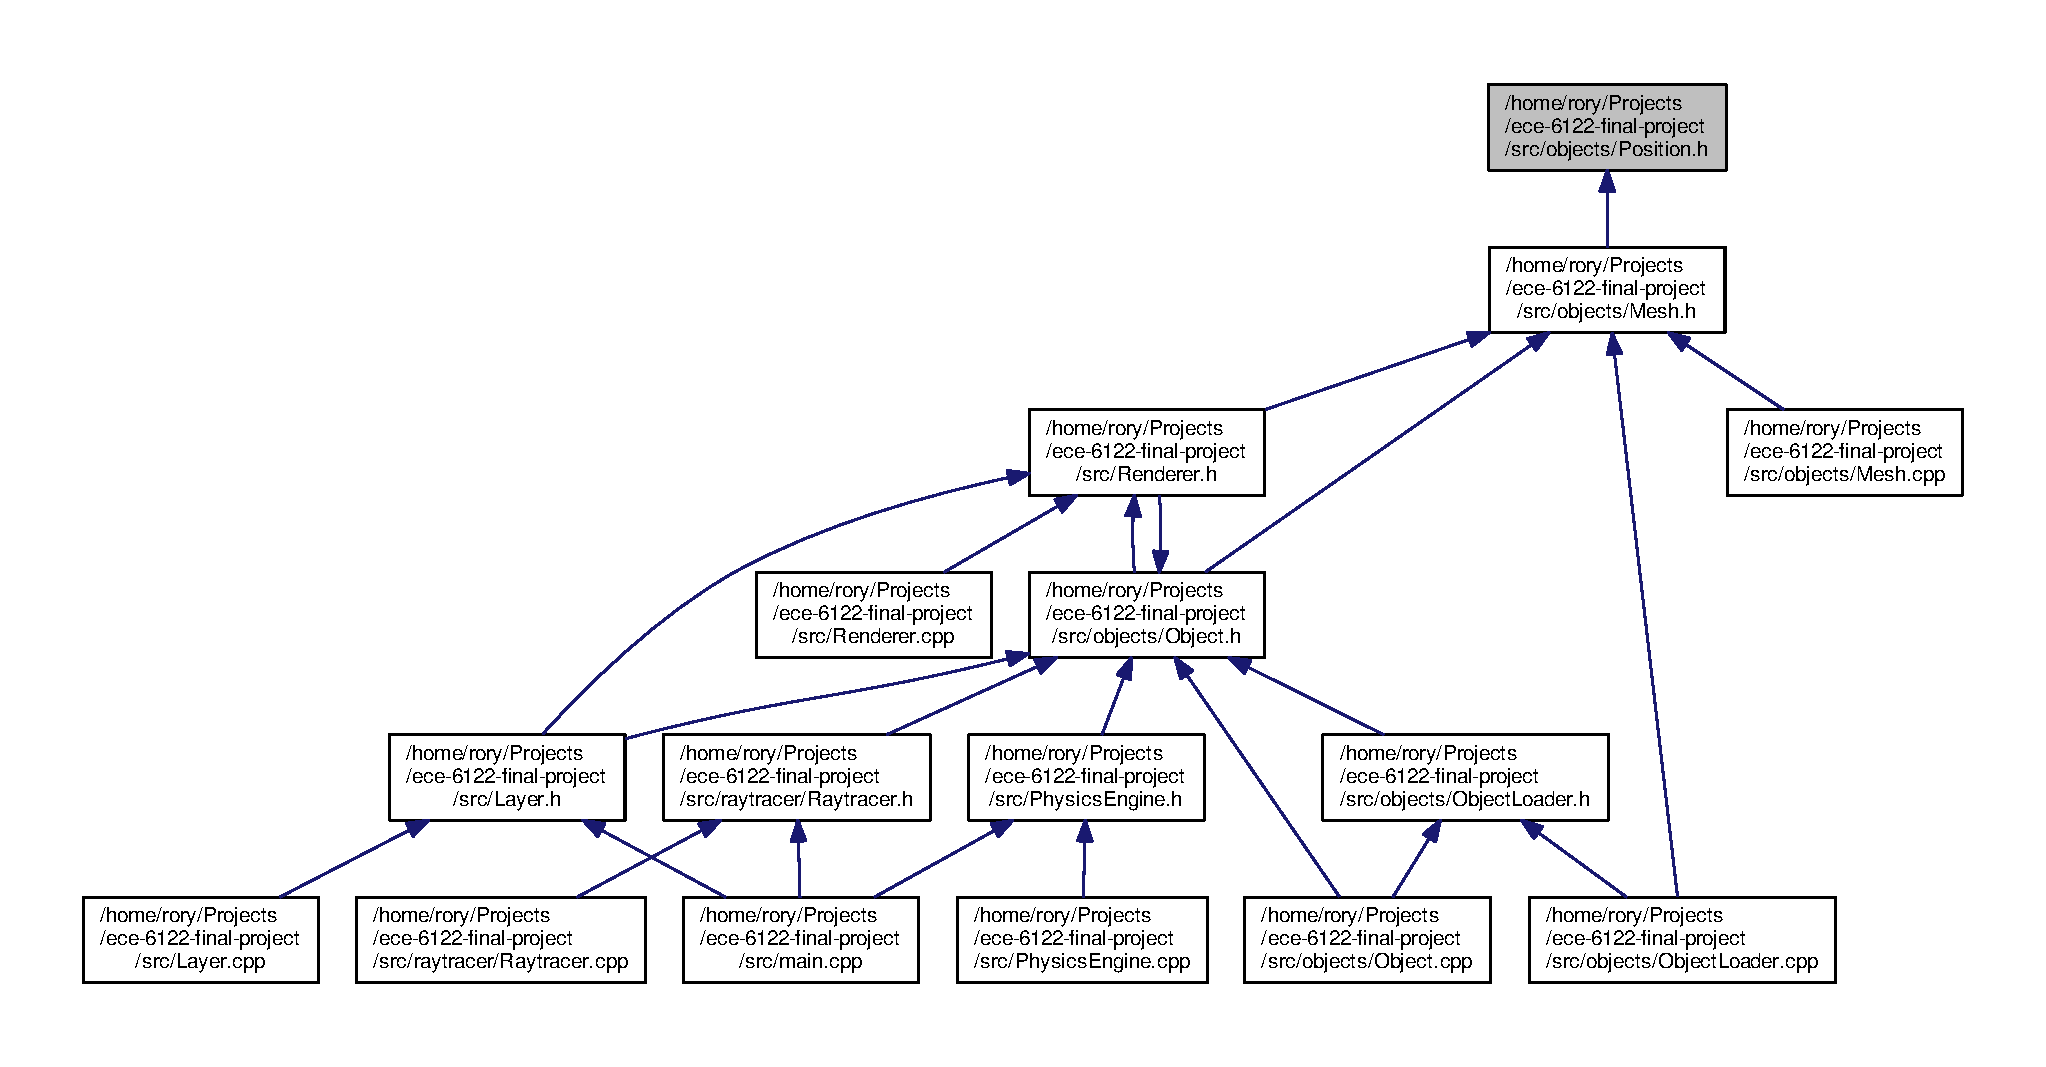
\includegraphics[width=350pt]{_position_8h__dep__incl}
\end{center}
\end{figure}
\subsection*{Classes}
\begin{DoxyCompactItemize}
\item 
struct \hyperlink{struct_position}{Position}
\end{DoxyCompactItemize}

\hypertarget{_tex_coord_8h}{}\section{/home/rory/\+Projects/ece-\/6122-\/final-\/project/src/objects/\+Tex\+Coord.h File Reference}
\label{_tex_coord_8h}\index{/home/rory/\+Projects/ece-\/6122-\/final-\/project/src/objects/\+Tex\+Coord.\+h@{/home/rory/\+Projects/ece-\/6122-\/final-\/project/src/objects/\+Tex\+Coord.\+h}}
{\ttfamily \#include $<$G\+L/glew.\+h$>$}\newline
{\ttfamily \#include $<$glm/glm.\+hpp$>$}\newline
Include dependency graph for Tex\+Coord.\+h\+:
\nopagebreak
\begin{figure}[H]
\begin{center}
\leavevmode
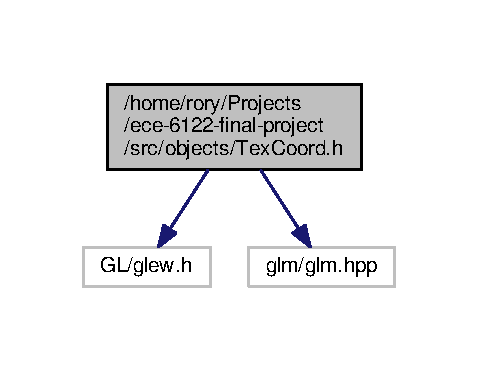
\includegraphics[width=230pt]{_tex_coord_8h__incl}
\end{center}
\end{figure}
This graph shows which files directly or indirectly include this file\+:
\nopagebreak
\begin{figure}[H]
\begin{center}
\leavevmode
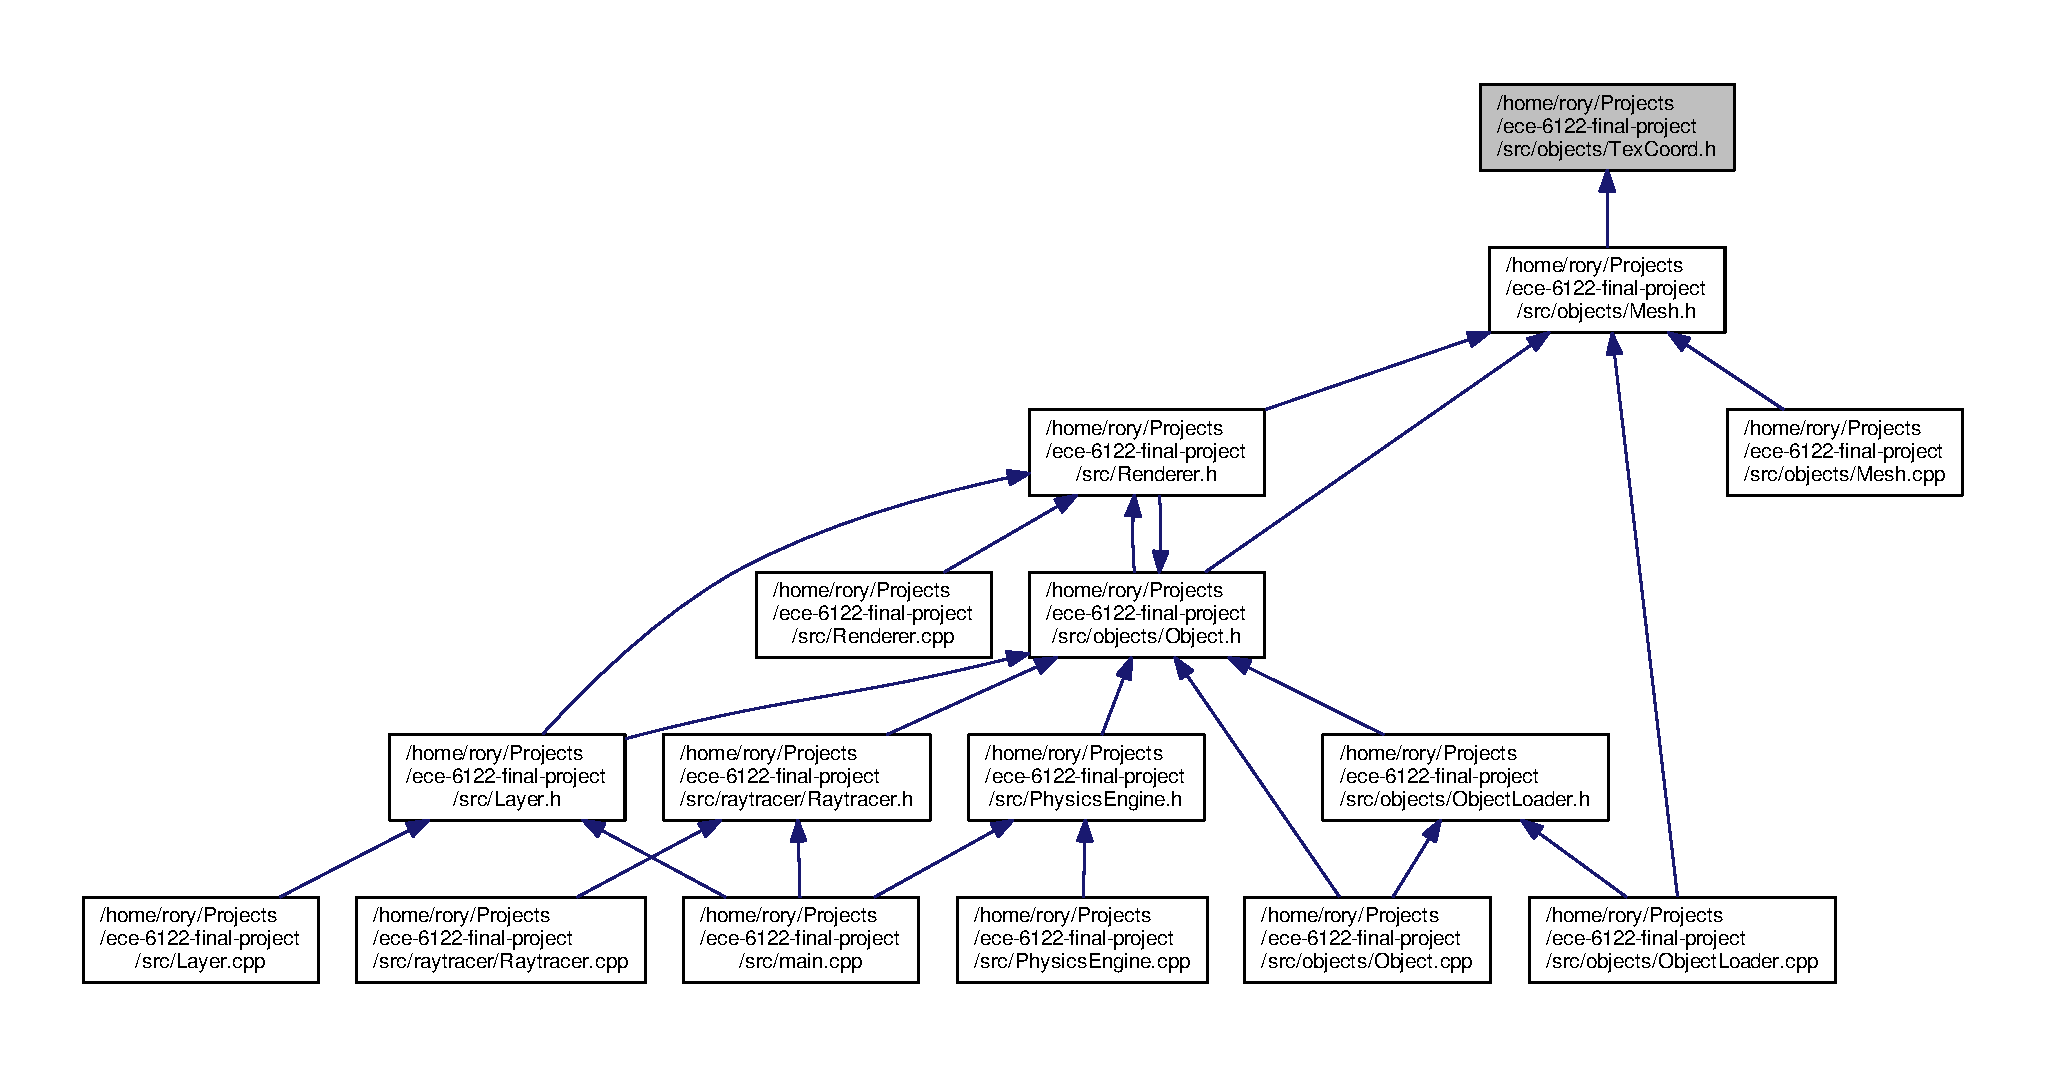
\includegraphics[width=350pt]{_tex_coord_8h__dep__incl}
\end{center}
\end{figure}
\subsection*{Classes}
\begin{DoxyCompactItemize}
\item 
struct \hyperlink{struct_tex_coord}{Tex\+Coord}
\end{DoxyCompactItemize}

\hypertarget{_texture_8cpp}{}\section{/home/rory/\+Projects/ece-\/6122-\/final-\/project/src/objects/\+Texture.cpp File Reference}
\label{_texture_8cpp}\index{/home/rory/\+Projects/ece-\/6122-\/final-\/project/src/objects/\+Texture.\+cpp@{/home/rory/\+Projects/ece-\/6122-\/final-\/project/src/objects/\+Texture.\+cpp}}
{\ttfamily \#include \char`\"{}Texture.\+h\char`\"{}}\newline
Include dependency graph for Texture.\+cpp\+:
\nopagebreak
\begin{figure}[H]
\begin{center}
\leavevmode
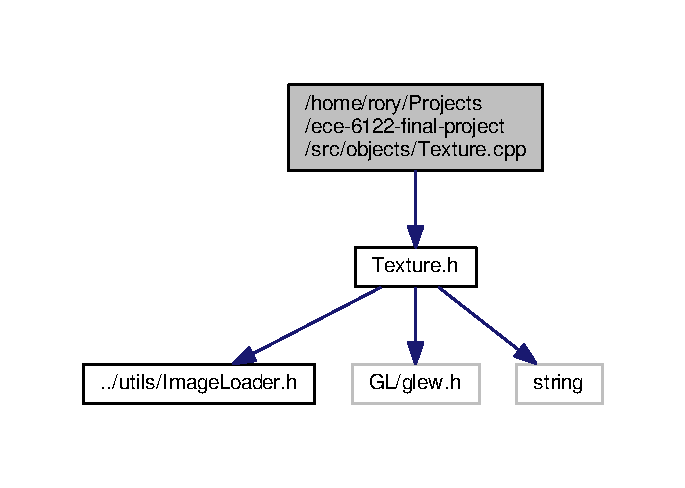
\includegraphics[width=329pt]{_texture_8cpp__incl}
\end{center}
\end{figure}

\hypertarget{_texture_8h}{}\section{/home/rory/\+Projects/ece-\/6122-\/final-\/project/src/objects/\+Texture.h File Reference}
\label{_texture_8h}\index{/home/rory/\+Projects/ece-\/6122-\/final-\/project/src/objects/\+Texture.\+h@{/home/rory/\+Projects/ece-\/6122-\/final-\/project/src/objects/\+Texture.\+h}}
{\ttfamily \#include \char`\"{}../utils/\+Image\+Loader.\+h\char`\"{}}\newline
{\ttfamily \#include $<$G\+L/glew.\+h$>$}\newline
{\ttfamily \#include $<$string$>$}\newline
Include dependency graph for Texture.\+h\+:
\nopagebreak
\begin{figure}[H]
\begin{center}
\leavevmode
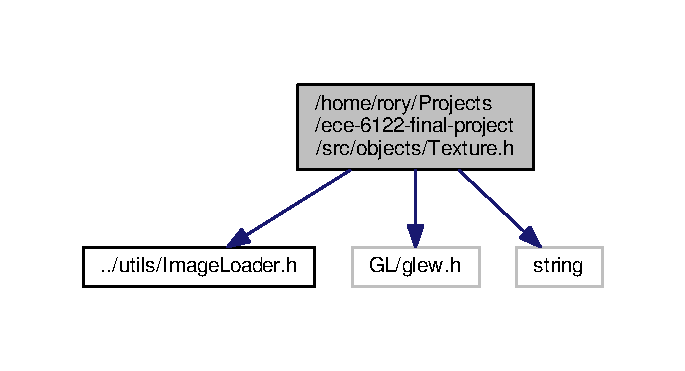
\includegraphics[width=329pt]{_texture_8h__incl}
\end{center}
\end{figure}
This graph shows which files directly or indirectly include this file\+:
\nopagebreak
\begin{figure}[H]
\begin{center}
\leavevmode
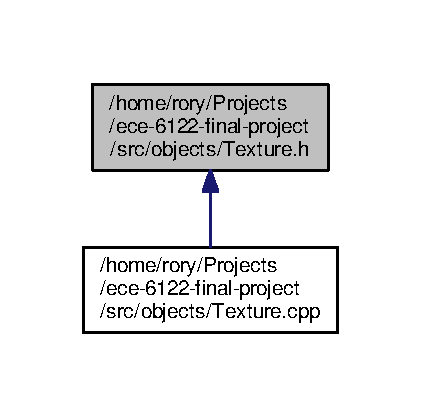
\includegraphics[width=202pt]{_texture_8h__dep__incl}
\end{center}
\end{figure}
\subsection*{Classes}
\begin{DoxyCompactItemize}
\item 
class \hyperlink{class_texture}{Texture}
\end{DoxyCompactItemize}

\hypertarget{_performance_data_8cpp}{}\section{/home/rory/\+Projects/ece-\/6122-\/final-\/project/src/\+Performance\+Data.cpp File Reference}
\label{_performance_data_8cpp}\index{/home/rory/\+Projects/ece-\/6122-\/final-\/project/src/\+Performance\+Data.\+cpp@{/home/rory/\+Projects/ece-\/6122-\/final-\/project/src/\+Performance\+Data.\+cpp}}
{\ttfamily \#include $<$cstring$>$}\newline
{\ttfamily \#include \char`\"{}Performance\+Data.\+h\char`\"{}}\newline
Include dependency graph for Performance\+Data.\+cpp\+:
\nopagebreak
\begin{figure}[H]
\begin{center}
\leavevmode
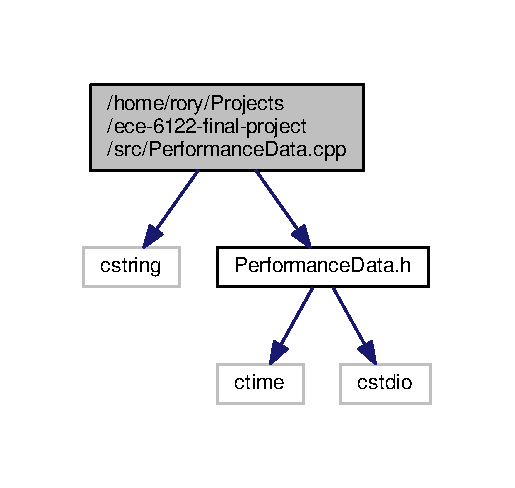
\includegraphics[width=247pt]{_performance_data_8cpp__incl}
\end{center}
\end{figure}

\hypertarget{_performance_data_8h}{}\section{/home/rory/\+Projects/ece-\/6122-\/final-\/project/src/\+Performance\+Data.h File Reference}
\label{_performance_data_8h}\index{/home/rory/\+Projects/ece-\/6122-\/final-\/project/src/\+Performance\+Data.\+h@{/home/rory/\+Projects/ece-\/6122-\/final-\/project/src/\+Performance\+Data.\+h}}
{\ttfamily \#include $<$ctime$>$}\newline
{\ttfamily \#include $<$cstdio$>$}\newline
Include dependency graph for Performance\+Data.\+h\+:
\nopagebreak
\begin{figure}[H]
\begin{center}
\leavevmode
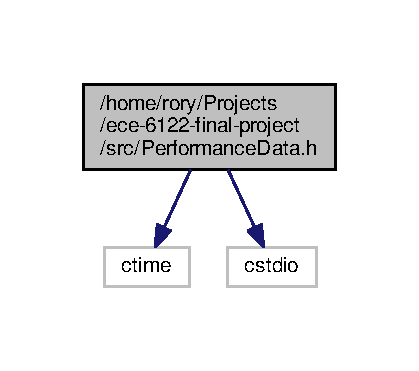
\includegraphics[width=201pt]{_performance_data_8h__incl}
\end{center}
\end{figure}
This graph shows which files directly or indirectly include this file\+:
\nopagebreak
\begin{figure}[H]
\begin{center}
\leavevmode
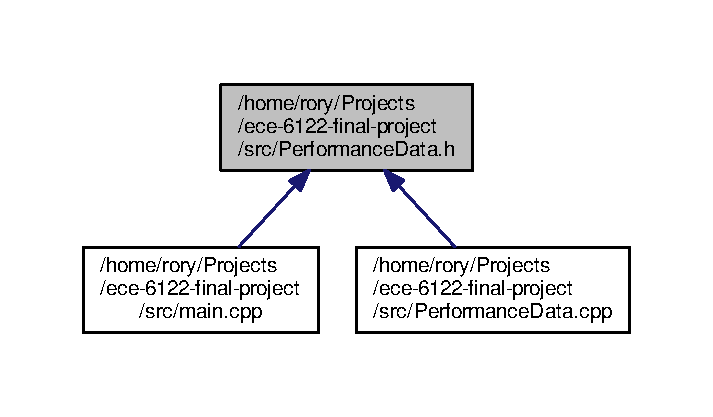
\includegraphics[width=342pt]{_performance_data_8h__dep__incl}
\end{center}
\end{figure}
\subsection*{Classes}
\begin{DoxyCompactItemize}
\item 
class \hyperlink{class_performance_data}{Performance\+Data}
\end{DoxyCompactItemize}

\hypertarget{_physics_engine_8cpp}{}\section{/home/rory/\+Projects/ece-\/6122-\/final-\/project/src/\+Physics\+Engine.cpp File Reference}
\label{_physics_engine_8cpp}\index{/home/rory/\+Projects/ece-\/6122-\/final-\/project/src/\+Physics\+Engine.\+cpp@{/home/rory/\+Projects/ece-\/6122-\/final-\/project/src/\+Physics\+Engine.\+cpp}}
{\ttfamily \#include \char`\"{}Physics\+Engine.\+h\char`\"{}}\newline
Include dependency graph for Physics\+Engine.\+cpp\+:
\nopagebreak
\begin{figure}[H]
\begin{center}
\leavevmode
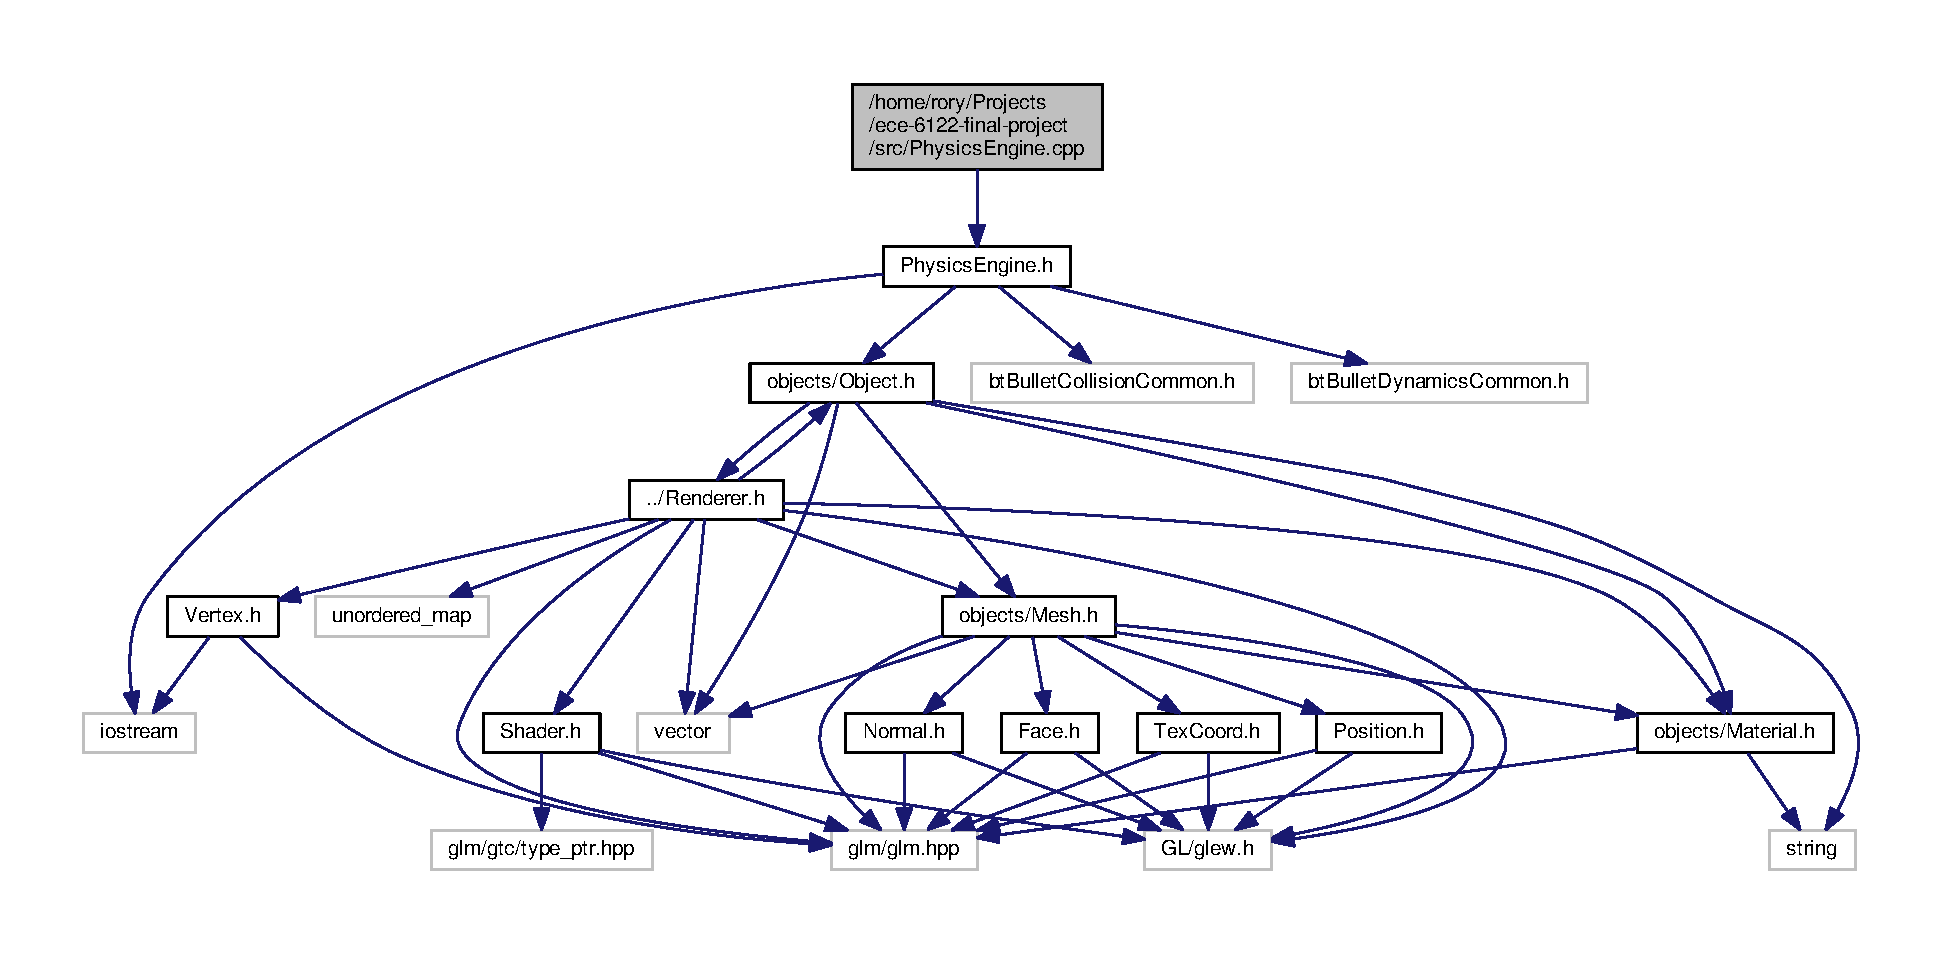
\includegraphics[width=350pt]{_physics_engine_8cpp__incl}
\end{center}
\end{figure}
\subsection*{Functions}
\begin{DoxyCompactItemize}
\item 
glm\+::mat4 \hyperlink{_physics_engine_8cpp_a0e5033658be58772df8bbca6b47f6eaf}{bt\+Scalar2glm\+Mat4} (bt\+Scalar $\ast$matrix)
\end{DoxyCompactItemize}


\subsection{Function Documentation}
\mbox{\Hypertarget{_physics_engine_8cpp_a0e5033658be58772df8bbca6b47f6eaf}\label{_physics_engine_8cpp_a0e5033658be58772df8bbca6b47f6eaf}} 
\index{Physics\+Engine.\+cpp@{Physics\+Engine.\+cpp}!bt\+Scalar2glm\+Mat4@{bt\+Scalar2glm\+Mat4}}
\index{bt\+Scalar2glm\+Mat4@{bt\+Scalar2glm\+Mat4}!Physics\+Engine.\+cpp@{Physics\+Engine.\+cpp}}
\subsubsection{\texorpdfstring{bt\+Scalar2glm\+Mat4()}{btScalar2glmMat4()}}
{\footnotesize\ttfamily glm\+::mat4 bt\+Scalar2glm\+Mat4 (\begin{DoxyParamCaption}\item[{bt\+Scalar $\ast$}]{matrix }\end{DoxyParamCaption})}

T\+O\+DO Document 
\begin{DoxyParams}{Parameters}
{\em matrix} & T\+O\+DO Document \\
\hline
\end{DoxyParams}
\begin{DoxyReturn}{Returns}
T\+O\+DO Document 
\end{DoxyReturn}


Definition at line 8 of file Physics\+Engine.\+cpp.


\hypertarget{_physics_engine_8h}{}\section{/home/rory/\+Projects/ece-\/6122-\/final-\/project/src/\+Physics\+Engine.h File Reference}
\label{_physics_engine_8h}\index{/home/rory/\+Projects/ece-\/6122-\/final-\/project/src/\+Physics\+Engine.\+h@{/home/rory/\+Projects/ece-\/6122-\/final-\/project/src/\+Physics\+Engine.\+h}}
{\ttfamily \#include \char`\"{}objects/\+Object.\+h\char`\"{}}\newline
{\ttfamily \#include $<$iostream$>$}\newline
{\ttfamily \#include $<$bt\+Bullet\+Collision\+Common.\+h$>$}\newline
{\ttfamily \#include $<$bt\+Bullet\+Dynamics\+Common.\+h$>$}\newline
Include dependency graph for Physics\+Engine.\+h\+:
\nopagebreak
\begin{figure}[H]
\begin{center}
\leavevmode
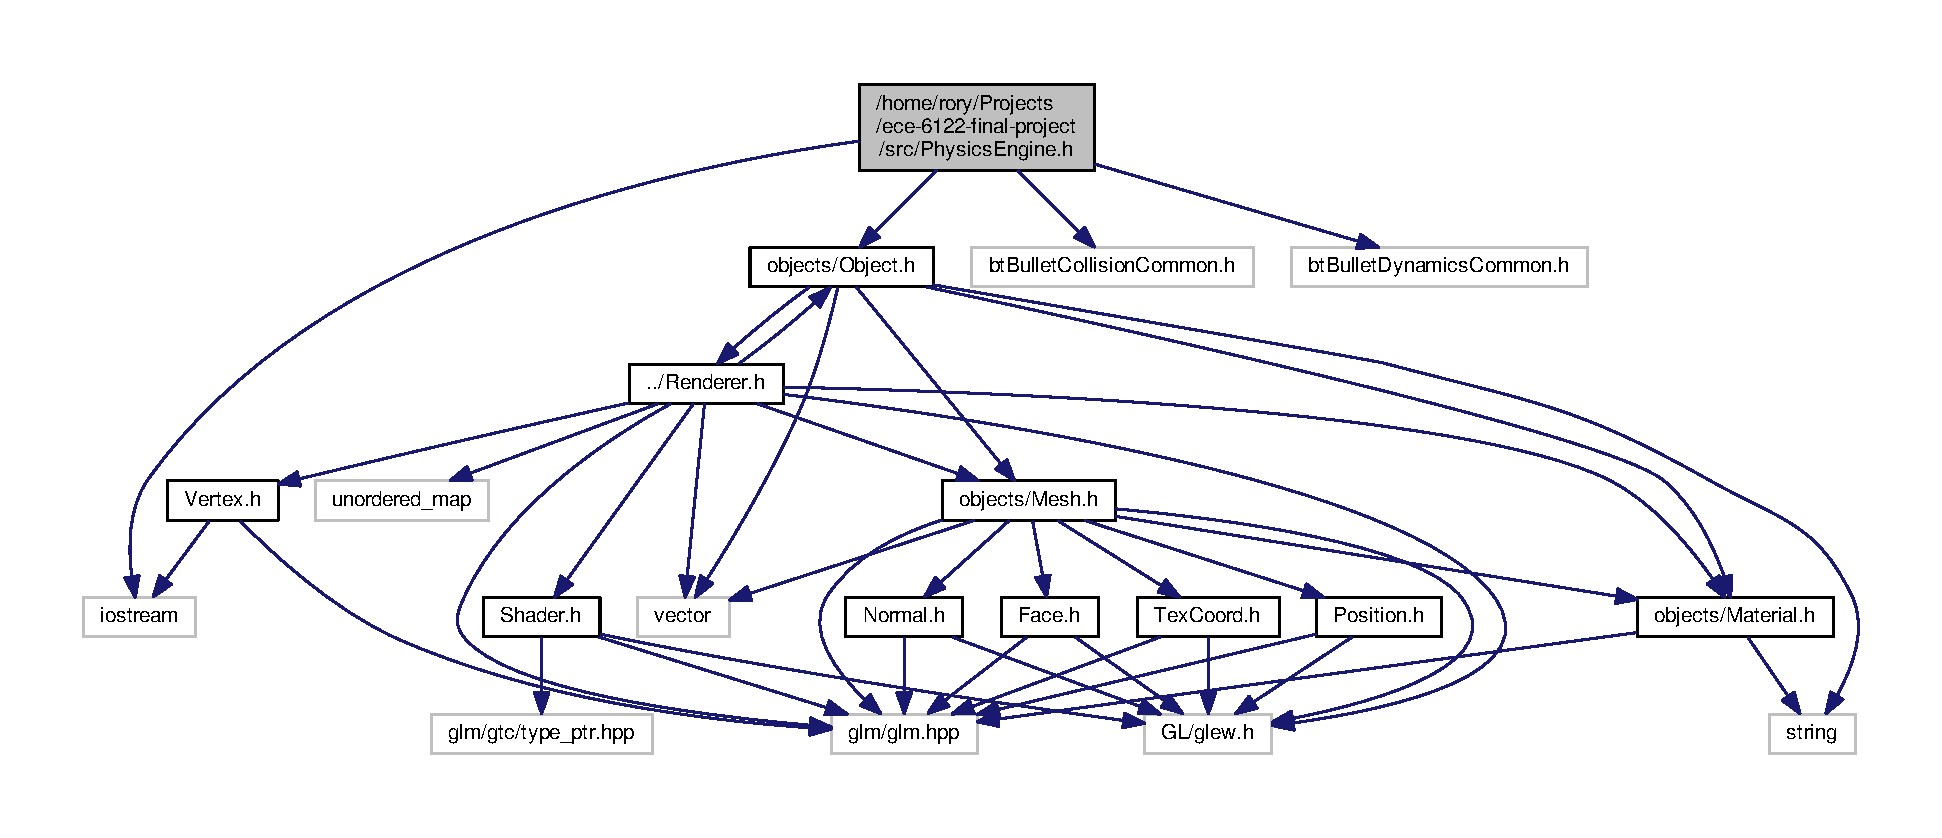
\includegraphics[width=350pt]{_physics_engine_8h__incl}
\end{center}
\end{figure}
This graph shows which files directly or indirectly include this file\+:
\nopagebreak
\begin{figure}[H]
\begin{center}
\leavevmode
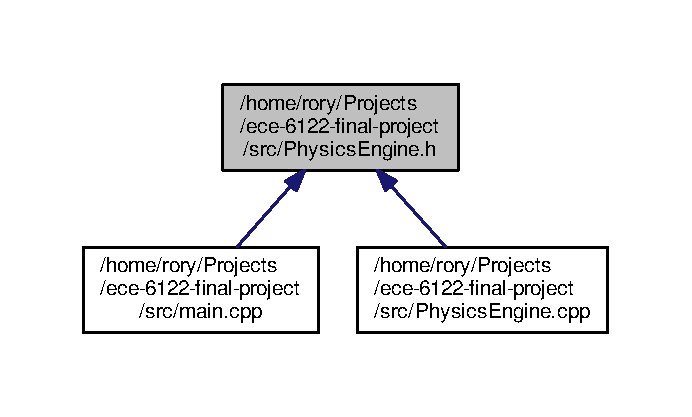
\includegraphics[width=332pt]{_physics_engine_8h__dep__incl}
\end{center}
\end{figure}
\subsection*{Classes}
\begin{DoxyCompactItemize}
\item 
class \hyperlink{class_physics_engine}{Physics\+Engine}
\end{DoxyCompactItemize}
\subsection*{Macros}
\begin{DoxyCompactItemize}
\item 
\#define \hyperlink{_physics_engine_8h_a17773d1969d6f5699a9317cfa2f89134}{D\+E\+F\+A\+U\+L\+T\+\_\+\+B\+O\+U\+N\+C\+I\+N\+E\+SS}~0.\+1f
\item 
\#define \hyperlink{_physics_engine_8h_aa6af90fbafcc281c7c546b1468369a9f}{D\+E\+F\+A\+U\+L\+T\+\_\+\+F\+R\+I\+C\+T\+I\+ON}~0.\+5f
\end{DoxyCompactItemize}


\subsection{Macro Definition Documentation}
\mbox{\Hypertarget{_physics_engine_8h_a17773d1969d6f5699a9317cfa2f89134}\label{_physics_engine_8h_a17773d1969d6f5699a9317cfa2f89134}} 
\index{Physics\+Engine.\+h@{Physics\+Engine.\+h}!D\+E\+F\+A\+U\+L\+T\+\_\+\+B\+O\+U\+N\+C\+I\+N\+E\+SS@{D\+E\+F\+A\+U\+L\+T\+\_\+\+B\+O\+U\+N\+C\+I\+N\+E\+SS}}
\index{D\+E\+F\+A\+U\+L\+T\+\_\+\+B\+O\+U\+N\+C\+I\+N\+E\+SS@{D\+E\+F\+A\+U\+L\+T\+\_\+\+B\+O\+U\+N\+C\+I\+N\+E\+SS}!Physics\+Engine.\+h@{Physics\+Engine.\+h}}
\subsubsection{\texorpdfstring{D\+E\+F\+A\+U\+L\+T\+\_\+\+B\+O\+U\+N\+C\+I\+N\+E\+SS}{DEFAULT\_BOUNCINESS}}
{\footnotesize\ttfamily \#define D\+E\+F\+A\+U\+L\+T\+\_\+\+B\+O\+U\+N\+C\+I\+N\+E\+SS~0.\+1f}



Definition at line 11 of file Physics\+Engine.\+h.

\mbox{\Hypertarget{_physics_engine_8h_aa6af90fbafcc281c7c546b1468369a9f}\label{_physics_engine_8h_aa6af90fbafcc281c7c546b1468369a9f}} 
\index{Physics\+Engine.\+h@{Physics\+Engine.\+h}!D\+E\+F\+A\+U\+L\+T\+\_\+\+F\+R\+I\+C\+T\+I\+ON@{D\+E\+F\+A\+U\+L\+T\+\_\+\+F\+R\+I\+C\+T\+I\+ON}}
\index{D\+E\+F\+A\+U\+L\+T\+\_\+\+F\+R\+I\+C\+T\+I\+ON@{D\+E\+F\+A\+U\+L\+T\+\_\+\+F\+R\+I\+C\+T\+I\+ON}!Physics\+Engine.\+h@{Physics\+Engine.\+h}}
\subsubsection{\texorpdfstring{D\+E\+F\+A\+U\+L\+T\+\_\+\+F\+R\+I\+C\+T\+I\+ON}{DEFAULT\_FRICTION}}
{\footnotesize\ttfamily \#define D\+E\+F\+A\+U\+L\+T\+\_\+\+F\+R\+I\+C\+T\+I\+ON~0.\+5f}



Definition at line 12 of file Physics\+Engine.\+h.


\hypertarget{_program_config_8h}{}\section{/home/rory/\+Projects/ece-\/6122-\/final-\/project/src/\+Program\+Config.h File Reference}
\label{_program_config_8h}\index{/home/rory/\+Projects/ece-\/6122-\/final-\/project/src/\+Program\+Config.\+h@{/home/rory/\+Projects/ece-\/6122-\/final-\/project/src/\+Program\+Config.\+h}}
{\ttfamily \#include $<$cstring$>$}\newline
{\ttfamily \#include $<$cstdio$>$}\newline
Include dependency graph for Program\+Config.\+h\+:
\nopagebreak
\begin{figure}[H]
\begin{center}
\leavevmode
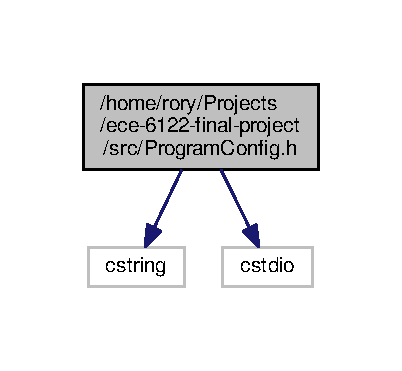
\includegraphics[width=193pt]{_program_config_8h__incl}
\end{center}
\end{figure}
This graph shows which files directly or indirectly include this file\+:
\nopagebreak
\begin{figure}[H]
\begin{center}
\leavevmode
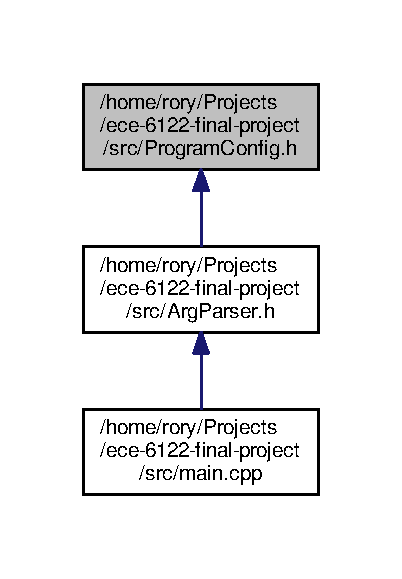
\includegraphics[width=193pt]{_program_config_8h__dep__incl}
\end{center}
\end{figure}
\subsection*{Classes}
\begin{DoxyCompactItemize}
\item 
struct \hyperlink{struct_program_config}{Program\+Config}
\end{DoxyCompactItemize}
\subsection*{Macros}
\begin{DoxyCompactItemize}
\item 
\#define \hyperlink{_program_config_8h_a3f8ed49c4045c1c273175f6205992687}{D\+E\+F\+A\+U\+L\+T\+\_\+\+M\+O\+V\+I\+E\+\_\+\+F\+I\+L\+E\+N\+A\+ME}~\char`\"{}movie.\+mpeg\char`\"{}
\end{DoxyCompactItemize}


\subsection{Macro Definition Documentation}
\mbox{\Hypertarget{_program_config_8h_a3f8ed49c4045c1c273175f6205992687}\label{_program_config_8h_a3f8ed49c4045c1c273175f6205992687}} 
\index{Program\+Config.\+h@{Program\+Config.\+h}!D\+E\+F\+A\+U\+L\+T\+\_\+\+M\+O\+V\+I\+E\+\_\+\+F\+I\+L\+E\+N\+A\+ME@{D\+E\+F\+A\+U\+L\+T\+\_\+\+M\+O\+V\+I\+E\+\_\+\+F\+I\+L\+E\+N\+A\+ME}}
\index{D\+E\+F\+A\+U\+L\+T\+\_\+\+M\+O\+V\+I\+E\+\_\+\+F\+I\+L\+E\+N\+A\+ME@{D\+E\+F\+A\+U\+L\+T\+\_\+\+M\+O\+V\+I\+E\+\_\+\+F\+I\+L\+E\+N\+A\+ME}!Program\+Config.\+h@{Program\+Config.\+h}}
\subsubsection{\texorpdfstring{D\+E\+F\+A\+U\+L\+T\+\_\+\+M\+O\+V\+I\+E\+\_\+\+F\+I\+L\+E\+N\+A\+ME}{DEFAULT\_MOVIE\_FILENAME}}
{\footnotesize\ttfamily \#define D\+E\+F\+A\+U\+L\+T\+\_\+\+M\+O\+V\+I\+E\+\_\+\+F\+I\+L\+E\+N\+A\+ME~\char`\"{}movie.\+mpeg\char`\"{}}



Definition at line 4 of file Program\+Config.\+h.


\hypertarget{_raytracer_8cpp}{}\section{/home/rory/\+Projects/ece-\/6122-\/final-\/project/src/raytracer/\+Raytracer.cpp File Reference}
\label{_raytracer_8cpp}\index{/home/rory/\+Projects/ece-\/6122-\/final-\/project/src/raytracer/\+Raytracer.\+cpp@{/home/rory/\+Projects/ece-\/6122-\/final-\/project/src/raytracer/\+Raytracer.\+cpp}}
{\ttfamily \#include \char`\"{}Raytracer.\+h\char`\"{}}\newline
{\ttfamily \#include \char`\"{}Sphere.\+h\char`\"{}}\newline
{\ttfamily \#include $<$stdlib.\+h$>$}\newline
{\ttfamily \#include $<$math.\+h$>$}\newline
{\ttfamily \#include $<$assert.\+h$>$}\newline
{\ttfamily \#include $<$fstream$>$}\newline
{\ttfamily \#include $<$vector$>$}\newline
{\ttfamily \#include $<$iostream$>$}\newline
{\ttfamily \#include $<$glm/glm.\+hpp$>$}\newline
Include dependency graph for Raytracer.\+cpp\+:
\nopagebreak
\begin{figure}[H]
\begin{center}
\leavevmode
\includegraphics[width=350pt]{_raytracer_8cpp__incl}
\end{center}
\end{figure}
\subsection*{Macros}
\begin{DoxyCompactItemize}
\item 
\#define \hyperlink{_raytracer_8cpp_a84517de5b8b5515dc6631fd07500751a}{M\+A\+X\+\_\+\+R\+A\+Y\+\_\+\+D\+E\+P\+TH}~25
\end{DoxyCompactItemize}
\subsection*{Functions}
\begin{DoxyCompactItemize}
\item 
float \hyperlink{_raytracer_8cpp_a874c09319b800d9eea74030236a3b4bc}{weight\+Distribution} (const float \&a, const float \&b, const float \&weight)
\item 
\hyperlink{_vector3_8h_af345ad77ba5e240c7ab72b4b2077e754}{Vector3f} \hyperlink{_raytracer_8cpp_ac0cc70e5f6a25d676cbcf2813d60c6a0}{trace} (const \hyperlink{_vector3_8h_af345ad77ba5e240c7ab72b4b2077e754}{Vector3f} \&ray\+Origin, const \hyperlink{_vector3_8h_af345ad77ba5e240c7ab72b4b2077e754}{Vector3f} \&ray\+Direction, const std\+::vector$<$ \hyperlink{class_sphere}{Sphere} $>$ \&spheres, const int \&depth)
\end{DoxyCompactItemize}


\subsection{Macro Definition Documentation}
\mbox{\Hypertarget{_raytracer_8cpp_a84517de5b8b5515dc6631fd07500751a}\label{_raytracer_8cpp_a84517de5b8b5515dc6631fd07500751a}} 
\index{Raytracer.\+cpp@{Raytracer.\+cpp}!M\+A\+X\+\_\+\+R\+A\+Y\+\_\+\+D\+E\+P\+TH@{M\+A\+X\+\_\+\+R\+A\+Y\+\_\+\+D\+E\+P\+TH}}
\index{M\+A\+X\+\_\+\+R\+A\+Y\+\_\+\+D\+E\+P\+TH@{M\+A\+X\+\_\+\+R\+A\+Y\+\_\+\+D\+E\+P\+TH}!Raytracer.\+cpp@{Raytracer.\+cpp}}
\subsubsection{\texorpdfstring{M\+A\+X\+\_\+\+R\+A\+Y\+\_\+\+D\+E\+P\+TH}{MAX\_RAY\_DEPTH}}
{\footnotesize\ttfamily \#define M\+A\+X\+\_\+\+R\+A\+Y\+\_\+\+D\+E\+P\+TH~25}



Definition at line 15 of file Raytracer.\+cpp.



\subsection{Function Documentation}
\mbox{\Hypertarget{_raytracer_8cpp_ac0cc70e5f6a25d676cbcf2813d60c6a0}\label{_raytracer_8cpp_ac0cc70e5f6a25d676cbcf2813d60c6a0}} 
\index{Raytracer.\+cpp@{Raytracer.\+cpp}!trace@{trace}}
\index{trace@{trace}!Raytracer.\+cpp@{Raytracer.\+cpp}}
\subsubsection{\texorpdfstring{trace()}{trace()}}
{\footnotesize\ttfamily \hyperlink{_vector3_8h_af345ad77ba5e240c7ab72b4b2077e754}{Vector3f} trace (\begin{DoxyParamCaption}\item[{const \hyperlink{_vector3_8h_af345ad77ba5e240c7ab72b4b2077e754}{Vector3f} \&}]{ray\+Origin,  }\item[{const \hyperlink{_vector3_8h_af345ad77ba5e240c7ab72b4b2077e754}{Vector3f} \&}]{ray\+Direction,  }\item[{const std\+::vector$<$ \hyperlink{class_sphere}{Sphere} $>$ \&}]{spheres,  }\item[{const int \&}]{depth }\end{DoxyParamCaption})}

The main trace function! It takes a standard ray as argument which is defined by its origin and direction. There is a test if this ray intersects any of the geometry in the scene (the geometry will be created later). If the ray intersects an object, the intersection point is computed, the normal at the intersection point is computed, and thus shade this point using this newly calculated information. Shading depends on the surface property of the primitive which is transparency, reflectiveness, diffuseablity. The function returns a color for the ray. If the ray intersects an object that is the color of the object at the intersection point, otherwise it returns the background color. 
\begin{DoxyParams}{Parameters}
{\em ray\+Origin} & T\+O\+DO Document \\
\hline
{\em ray\+Direction} & T\+O\+DO Document \\
\hline
{\em spheres} & T\+O\+DO Document \\
\hline
{\em depth} & T\+O\+DO Document \\
\hline
\end{DoxyParams}
\begin{DoxyReturn}{Returns}
T\+O\+DO Document 
\end{DoxyReturn}


Definition at line 46 of file Raytracer.\+cpp.

\mbox{\Hypertarget{_raytracer_8cpp_a874c09319b800d9eea74030236a3b4bc}\label{_raytracer_8cpp_a874c09319b800d9eea74030236a3b4bc}} 
\index{Raytracer.\+cpp@{Raytracer.\+cpp}!weight\+Distribution@{weight\+Distribution}}
\index{weight\+Distribution@{weight\+Distribution}!Raytracer.\+cpp@{Raytracer.\+cpp}}
\subsubsection{\texorpdfstring{weight\+Distribution()}{weightDistribution()}}
{\footnotesize\ttfamily float weight\+Distribution (\begin{DoxyParamCaption}\item[{const float \&}]{a,  }\item[{const float \&}]{b,  }\item[{const float \&}]{weight }\end{DoxyParamCaption})}

Helper function for color mixing based on weight 
\begin{DoxyParams}{Parameters}
{\em a} & T\+O\+DO Document \\
\hline
{\em b} & T\+O\+DO Document \\
\hline
{\em weight} & T\+O\+DO Document \\
\hline
\end{DoxyParams}
\begin{DoxyReturn}{Returns}
T\+O\+DO Document 
\end{DoxyReturn}


Definition at line 24 of file Raytracer.\+cpp.


\hypertarget{_raytracer_8h}{}\section{/home/rory/\+Projects/ece-\/6122-\/final-\/project/src/raytracer/\+Raytracer.h File Reference}
\label{_raytracer_8h}\index{/home/rory/\+Projects/ece-\/6122-\/final-\/project/src/raytracer/\+Raytracer.\+h@{/home/rory/\+Projects/ece-\/6122-\/final-\/project/src/raytracer/\+Raytracer.\+h}}
{\ttfamily \#include \char`\"{}Sphere.\+h\char`\"{}}\newline
{\ttfamily \#include \char`\"{}Vector3.\+h\char`\"{}}\newline
{\ttfamily \#include \char`\"{}../objects/\+Object.\+h\char`\"{}}\newline
{\ttfamily \#include $<$vector$>$}\newline
Include dependency graph for Raytracer.\+h\+:
\nopagebreak
\begin{figure}[H]
\begin{center}
\leavevmode
\includegraphics[width=350pt]{_raytracer_8h__incl}
\end{center}
\end{figure}
This graph shows which files directly or indirectly include this file\+:
\nopagebreak
\begin{figure}[H]
\begin{center}
\leavevmode
\includegraphics[width=350pt]{_raytracer_8h__dep__incl}
\end{center}
\end{figure}
\subsection*{Classes}
\begin{DoxyCompactItemize}
\item 
class \hyperlink{class_raytracer}{Raytracer}
\end{DoxyCompactItemize}

\hypertarget{_sphere_8h}{}\section{/home/rory/\+Projects/ece-\/6122-\/final-\/project/src/raytracer/\+Sphere.h File Reference}
\label{_sphere_8h}\index{/home/rory/\+Projects/ece-\/6122-\/final-\/project/src/raytracer/\+Sphere.\+h@{/home/rory/\+Projects/ece-\/6122-\/final-\/project/src/raytracer/\+Sphere.\+h}}
{\ttfamily \#include \char`\"{}Vector3.\+h\char`\"{}}\newline
Include dependency graph for Sphere.\+h\+:
\nopagebreak
\begin{figure}[H]
\begin{center}
\leavevmode
\includegraphics[width=199pt]{_sphere_8h__incl}
\end{center}
\end{figure}
This graph shows which files directly or indirectly include this file\+:
\nopagebreak
\begin{figure}[H]
\begin{center}
\leavevmode
\includegraphics[width=350pt]{_sphere_8h__dep__incl}
\end{center}
\end{figure}
\subsection*{Classes}
\begin{DoxyCompactItemize}
\item 
class \hyperlink{class_sphere}{Sphere}
\end{DoxyCompactItemize}

\hypertarget{_vector3_8h}{}\section{/home/rory/\+Projects/ece-\/6122-\/final-\/project/src/raytracer/\+Vector3.h File Reference}
\label{_vector3_8h}\index{/home/rory/\+Projects/ece-\/6122-\/final-\/project/src/raytracer/\+Vector3.\+h@{/home/rory/\+Projects/ece-\/6122-\/final-\/project/src/raytracer/\+Vector3.\+h}}
{\ttfamily \#include $<$cmath$>$}\newline
{\ttfamily \#include $<$iostream$>$}\newline
Include dependency graph for Vector3.\+h\+:
\nopagebreak
\begin{figure}[H]
\begin{center}
\leavevmode
\includegraphics[width=201pt]{_vector3_8h__incl}
\end{center}
\end{figure}
This graph shows which files directly or indirectly include this file\+:
\nopagebreak
\begin{figure}[H]
\begin{center}
\leavevmode
\includegraphics[width=350pt]{_vector3_8h__dep__incl}
\end{center}
\end{figure}
\subsection*{Classes}
\begin{DoxyCompactItemize}
\item 
class \hyperlink{class_vector3}{Vector3$<$ Tvalue $>$}
\end{DoxyCompactItemize}
\subsection*{Typedefs}
\begin{DoxyCompactItemize}
\item 
typedef \hyperlink{class_vector3}{Vector3}$<$ float $>$ \hyperlink{_vector3_8h_af345ad77ba5e240c7ab72b4b2077e754}{Vector3f}
\end{DoxyCompactItemize}


\subsection{Typedef Documentation}
\mbox{\Hypertarget{_vector3_8h_af345ad77ba5e240c7ab72b4b2077e754}\label{_vector3_8h_af345ad77ba5e240c7ab72b4b2077e754}} 
\index{Vector3.\+h@{Vector3.\+h}!Vector3f@{Vector3f}}
\index{Vector3f@{Vector3f}!Vector3.\+h@{Vector3.\+h}}
\subsubsection{\texorpdfstring{Vector3f}{Vector3f}}
{\footnotesize\ttfamily typedef \hyperlink{class_vector3}{Vector3}$<$float$>$ \hyperlink{_vector3_8h_af345ad77ba5e240c7ab72b4b2077e754}{Vector3f}}



Definition at line 64 of file Vector3.\+h.


\hypertarget{_renderer_8cpp}{}\section{/home/rory/\+Projects/ece-\/6122-\/final-\/project/src/\+Renderer.cpp File Reference}
\label{_renderer_8cpp}\index{/home/rory/\+Projects/ece-\/6122-\/final-\/project/src/\+Renderer.\+cpp@{/home/rory/\+Projects/ece-\/6122-\/final-\/project/src/\+Renderer.\+cpp}}
{\ttfamily \#include \char`\"{}Renderer.\+h\char`\"{}}\newline
{\ttfamily \#include \char`\"{}objects/\+Color.\+h\char`\"{}}\newline
{\ttfamily \#include $<$algorithm$>$}\newline
Include dependency graph for Renderer.\+cpp\+:
\nopagebreak
\begin{figure}[H]
\begin{center}
\leavevmode
\includegraphics[width=350pt]{_renderer_8cpp__incl}
\end{center}
\end{figure}

\hypertarget{_renderer_8h}{}\section{/home/rory/\+Projects/ece-\/6122-\/final-\/project/src/\+Renderer.h File Reference}
\label{_renderer_8h}\index{/home/rory/\+Projects/ece-\/6122-\/final-\/project/src/\+Renderer.\+h@{/home/rory/\+Projects/ece-\/6122-\/final-\/project/src/\+Renderer.\+h}}
{\ttfamily \#include \char`\"{}Vertex.\+h\char`\"{}}\newline
{\ttfamily \#include \char`\"{}Shader.\+h\char`\"{}}\newline
{\ttfamily \#include \char`\"{}objects/\+Material.\+h\char`\"{}}\newline
{\ttfamily \#include \char`\"{}objects/\+Object.\+h\char`\"{}}\newline
{\ttfamily \#include $<$G\+L/glew.\+h$>$}\newline
{\ttfamily \#include $<$glm/glm.\+hpp$>$}\newline
{\ttfamily \#include $<$vector$>$}\newline
{\ttfamily \#include $<$unordered\+\_\+map$>$}\newline
{\ttfamily \#include \char`\"{}objects/\+Mesh.\+h\char`\"{}}\newline
Include dependency graph for Renderer.\+h\+:
\nopagebreak
\begin{figure}[H]
\begin{center}
\leavevmode
\includegraphics[width=350pt]{_renderer_8h__incl}
\end{center}
\end{figure}
This graph shows which files directly or indirectly include this file\+:
\nopagebreak
\begin{figure}[H]
\begin{center}
\leavevmode
\includegraphics[width=350pt]{_renderer_8h__dep__incl}
\end{center}
\end{figure}
\subsection*{Classes}
\begin{DoxyCompactItemize}
\item 
class \hyperlink{class_renderer}{Renderer}
\end{DoxyCompactItemize}
\subsection*{Macros}
\begin{DoxyCompactItemize}
\item 
\#define \hyperlink{_renderer_8h_a1222715d70ab6ad1c82a6effafc04f50}{M\+E\+S\+H\+\_\+\+M\+A\+X\+\_\+\+I\+N\+D\+I\+C\+ES}~1000000
\item 
\#define \hyperlink{_renderer_8h_ab708ba001cad140d470df55643718f9a}{M\+E\+S\+H\+\_\+\+M\+A\+X\+\_\+\+B\+U\+F\+F\+E\+R\+\_\+\+B\+Y\+T\+ES}~1000000
\item 
\#define \hyperlink{_renderer_8h_aaa7dbbfc587f9c9270b26b71f6e52c9d}{S\+H\+A\+D\+E\+R\+\_\+\+I\+N\+D\+E\+X\+\_\+\+P\+O\+S\+I\+T\+I\+ON}~0
\item 
\#define \hyperlink{_renderer_8h_afb97290f0bc78c2373fdddd65f8c4385}{S\+H\+A\+D\+E\+R\+\_\+\+I\+N\+D\+E\+X\+\_\+\+UV}~1
\item 
\#define \hyperlink{_renderer_8h_a9f231c0b3172592598f8dbbca1108ab2}{S\+H\+A\+D\+E\+R\+\_\+\+I\+N\+D\+E\+X\+\_\+\+C\+O\+L\+OR}~2
\item 
\#define \hyperlink{_renderer_8h_af1814c4492cd4c2ddc46f0f7ad9dcbad}{S\+H\+A\+D\+E\+R\+\_\+\+I\+N\+D\+E\+X\+\_\+\+N\+O\+R\+M\+AL}~3
\end{DoxyCompactItemize}


\subsection{Macro Definition Documentation}
\mbox{\Hypertarget{_renderer_8h_ab708ba001cad140d470df55643718f9a}\label{_renderer_8h_ab708ba001cad140d470df55643718f9a}} 
\index{Renderer.\+h@{Renderer.\+h}!M\+E\+S\+H\+\_\+\+M\+A\+X\+\_\+\+B\+U\+F\+F\+E\+R\+\_\+\+B\+Y\+T\+ES@{M\+E\+S\+H\+\_\+\+M\+A\+X\+\_\+\+B\+U\+F\+F\+E\+R\+\_\+\+B\+Y\+T\+ES}}
\index{M\+E\+S\+H\+\_\+\+M\+A\+X\+\_\+\+B\+U\+F\+F\+E\+R\+\_\+\+B\+Y\+T\+ES@{M\+E\+S\+H\+\_\+\+M\+A\+X\+\_\+\+B\+U\+F\+F\+E\+R\+\_\+\+B\+Y\+T\+ES}!Renderer.\+h@{Renderer.\+h}}
\subsubsection{\texorpdfstring{M\+E\+S\+H\+\_\+\+M\+A\+X\+\_\+\+B\+U\+F\+F\+E\+R\+\_\+\+B\+Y\+T\+ES}{MESH\_MAX\_BUFFER\_BYTES}}
{\footnotesize\ttfamily \#define M\+E\+S\+H\+\_\+\+M\+A\+X\+\_\+\+B\+U\+F\+F\+E\+R\+\_\+\+B\+Y\+T\+ES~1000000}



Definition at line 15 of file Renderer.\+h.

\mbox{\Hypertarget{_renderer_8h_a1222715d70ab6ad1c82a6effafc04f50}\label{_renderer_8h_a1222715d70ab6ad1c82a6effafc04f50}} 
\index{Renderer.\+h@{Renderer.\+h}!M\+E\+S\+H\+\_\+\+M\+A\+X\+\_\+\+I\+N\+D\+I\+C\+ES@{M\+E\+S\+H\+\_\+\+M\+A\+X\+\_\+\+I\+N\+D\+I\+C\+ES}}
\index{M\+E\+S\+H\+\_\+\+M\+A\+X\+\_\+\+I\+N\+D\+I\+C\+ES@{M\+E\+S\+H\+\_\+\+M\+A\+X\+\_\+\+I\+N\+D\+I\+C\+ES}!Renderer.\+h@{Renderer.\+h}}
\subsubsection{\texorpdfstring{M\+E\+S\+H\+\_\+\+M\+A\+X\+\_\+\+I\+N\+D\+I\+C\+ES}{MESH\_MAX\_INDICES}}
{\footnotesize\ttfamily \#define M\+E\+S\+H\+\_\+\+M\+A\+X\+\_\+\+I\+N\+D\+I\+C\+ES~1000000}



Definition at line 14 of file Renderer.\+h.

\mbox{\Hypertarget{_renderer_8h_a9f231c0b3172592598f8dbbca1108ab2}\label{_renderer_8h_a9f231c0b3172592598f8dbbca1108ab2}} 
\index{Renderer.\+h@{Renderer.\+h}!S\+H\+A\+D\+E\+R\+\_\+\+I\+N\+D\+E\+X\+\_\+\+C\+O\+L\+OR@{S\+H\+A\+D\+E\+R\+\_\+\+I\+N\+D\+E\+X\+\_\+\+C\+O\+L\+OR}}
\index{S\+H\+A\+D\+E\+R\+\_\+\+I\+N\+D\+E\+X\+\_\+\+C\+O\+L\+OR@{S\+H\+A\+D\+E\+R\+\_\+\+I\+N\+D\+E\+X\+\_\+\+C\+O\+L\+OR}!Renderer.\+h@{Renderer.\+h}}
\subsubsection{\texorpdfstring{S\+H\+A\+D\+E\+R\+\_\+\+I\+N\+D\+E\+X\+\_\+\+C\+O\+L\+OR}{SHADER\_INDEX\_COLOR}}
{\footnotesize\ttfamily \#define S\+H\+A\+D\+E\+R\+\_\+\+I\+N\+D\+E\+X\+\_\+\+C\+O\+L\+OR~2}



Definition at line 19 of file Renderer.\+h.

\mbox{\Hypertarget{_renderer_8h_af1814c4492cd4c2ddc46f0f7ad9dcbad}\label{_renderer_8h_af1814c4492cd4c2ddc46f0f7ad9dcbad}} 
\index{Renderer.\+h@{Renderer.\+h}!S\+H\+A\+D\+E\+R\+\_\+\+I\+N\+D\+E\+X\+\_\+\+N\+O\+R\+M\+AL@{S\+H\+A\+D\+E\+R\+\_\+\+I\+N\+D\+E\+X\+\_\+\+N\+O\+R\+M\+AL}}
\index{S\+H\+A\+D\+E\+R\+\_\+\+I\+N\+D\+E\+X\+\_\+\+N\+O\+R\+M\+AL@{S\+H\+A\+D\+E\+R\+\_\+\+I\+N\+D\+E\+X\+\_\+\+N\+O\+R\+M\+AL}!Renderer.\+h@{Renderer.\+h}}
\subsubsection{\texorpdfstring{S\+H\+A\+D\+E\+R\+\_\+\+I\+N\+D\+E\+X\+\_\+\+N\+O\+R\+M\+AL}{SHADER\_INDEX\_NORMAL}}
{\footnotesize\ttfamily \#define S\+H\+A\+D\+E\+R\+\_\+\+I\+N\+D\+E\+X\+\_\+\+N\+O\+R\+M\+AL~3}



Definition at line 20 of file Renderer.\+h.

\mbox{\Hypertarget{_renderer_8h_aaa7dbbfc587f9c9270b26b71f6e52c9d}\label{_renderer_8h_aaa7dbbfc587f9c9270b26b71f6e52c9d}} 
\index{Renderer.\+h@{Renderer.\+h}!S\+H\+A\+D\+E\+R\+\_\+\+I\+N\+D\+E\+X\+\_\+\+P\+O\+S\+I\+T\+I\+ON@{S\+H\+A\+D\+E\+R\+\_\+\+I\+N\+D\+E\+X\+\_\+\+P\+O\+S\+I\+T\+I\+ON}}
\index{S\+H\+A\+D\+E\+R\+\_\+\+I\+N\+D\+E\+X\+\_\+\+P\+O\+S\+I\+T\+I\+ON@{S\+H\+A\+D\+E\+R\+\_\+\+I\+N\+D\+E\+X\+\_\+\+P\+O\+S\+I\+T\+I\+ON}!Renderer.\+h@{Renderer.\+h}}
\subsubsection{\texorpdfstring{S\+H\+A\+D\+E\+R\+\_\+\+I\+N\+D\+E\+X\+\_\+\+P\+O\+S\+I\+T\+I\+ON}{SHADER\_INDEX\_POSITION}}
{\footnotesize\ttfamily \#define S\+H\+A\+D\+E\+R\+\_\+\+I\+N\+D\+E\+X\+\_\+\+P\+O\+S\+I\+T\+I\+ON~0}



Definition at line 17 of file Renderer.\+h.

\mbox{\Hypertarget{_renderer_8h_afb97290f0bc78c2373fdddd65f8c4385}\label{_renderer_8h_afb97290f0bc78c2373fdddd65f8c4385}} 
\index{Renderer.\+h@{Renderer.\+h}!S\+H\+A\+D\+E\+R\+\_\+\+I\+N\+D\+E\+X\+\_\+\+UV@{S\+H\+A\+D\+E\+R\+\_\+\+I\+N\+D\+E\+X\+\_\+\+UV}}
\index{S\+H\+A\+D\+E\+R\+\_\+\+I\+N\+D\+E\+X\+\_\+\+UV@{S\+H\+A\+D\+E\+R\+\_\+\+I\+N\+D\+E\+X\+\_\+\+UV}!Renderer.\+h@{Renderer.\+h}}
\subsubsection{\texorpdfstring{S\+H\+A\+D\+E\+R\+\_\+\+I\+N\+D\+E\+X\+\_\+\+UV}{SHADER\_INDEX\_UV}}
{\footnotesize\ttfamily \#define S\+H\+A\+D\+E\+R\+\_\+\+I\+N\+D\+E\+X\+\_\+\+UV~1}



Definition at line 18 of file Renderer.\+h.


\hypertarget{_shader_8cpp}{}\section{/home/rory/\+Projects/ece-\/6122-\/final-\/project/src/\+Shader.cpp File Reference}
\label{_shader_8cpp}\index{/home/rory/\+Projects/ece-\/6122-\/final-\/project/src/\+Shader.\+cpp@{/home/rory/\+Projects/ece-\/6122-\/final-\/project/src/\+Shader.\+cpp}}
{\ttfamily \#include \char`\"{}Shader.\+h\char`\"{}}\newline
{\ttfamily \#include $<$string$>$}\newline
{\ttfamily \#include $<$vector$>$}\newline
{\ttfamily \#include $<$cstdio$>$}\newline
Include dependency graph for Shader.\+cpp\+:
\nopagebreak
\begin{figure}[H]
\begin{center}
\leavevmode
\includegraphics[width=350pt]{_shader_8cpp__incl}
\end{center}
\end{figure}
\subsection*{Functions}
\begin{DoxyCompactItemize}
\item 
std\+::string \hyperlink{_shader_8cpp_a931761b66c39b5cebcf889064ab4ee1c}{read\+\_\+file} (const char $\ast$filepath)
\end{DoxyCompactItemize}


\subsection{Function Documentation}
\mbox{\Hypertarget{_shader_8cpp_a931761b66c39b5cebcf889064ab4ee1c}\label{_shader_8cpp_a931761b66c39b5cebcf889064ab4ee1c}} 
\index{Shader.\+cpp@{Shader.\+cpp}!read\+\_\+file@{read\+\_\+file}}
\index{read\+\_\+file@{read\+\_\+file}!Shader.\+cpp@{Shader.\+cpp}}
\subsubsection{\texorpdfstring{read\+\_\+file()}{read\_file()}}
{\footnotesize\ttfamily std\+::string read\+\_\+file (\begin{DoxyParamCaption}\item[{const char $\ast$}]{filepath }\end{DoxyParamCaption})}

Returns the contents of the file at the specified path 
\begin{DoxyParams}{Parameters}
{\em filepath} & The path of the file to read \\
\hline
\end{DoxyParams}
\begin{DoxyReturn}{Returns}
Returns the contents of the file on success, else an empty string on error 
\end{DoxyReturn}


Definition at line 236 of file Shader.\+cpp.


\hypertarget{_shader_8h}{}\section{/home/rory/\+Projects/ece-\/6122-\/final-\/project/src/\+Shader.h File Reference}
\label{_shader_8h}\index{/home/rory/\+Projects/ece-\/6122-\/final-\/project/src/\+Shader.\+h@{/home/rory/\+Projects/ece-\/6122-\/final-\/project/src/\+Shader.\+h}}
{\ttfamily \#include $<$G\+L/glew.\+h$>$}\newline
{\ttfamily \#include $<$glm/glm.\+hpp$>$}\newline
{\ttfamily \#include $<$glm/gtc/type\+\_\+ptr.\+hpp$>$}\newline
Include dependency graph for Shader.\+h\+:
\nopagebreak
\begin{figure}[H]
\begin{center}
\leavevmode
\includegraphics[width=350pt]{_shader_8h__incl}
\end{center}
\end{figure}
This graph shows which files directly or indirectly include this file\+:
\nopagebreak
\begin{figure}[H]
\begin{center}
\leavevmode
\includegraphics[width=350pt]{_shader_8h__dep__incl}
\end{center}
\end{figure}
\subsection*{Classes}
\begin{DoxyCompactItemize}
\item 
class \hyperlink{class_shader}{Shader}
\end{DoxyCompactItemize}

\hypertarget{_text_writer_8cpp}{}\section{/home/rory/\+Projects/ece-\/6122-\/final-\/project/src/\+Text\+Writer.cpp File Reference}
\label{_text_writer_8cpp}\index{/home/rory/\+Projects/ece-\/6122-\/final-\/project/src/\+Text\+Writer.\+cpp@{/home/rory/\+Projects/ece-\/6122-\/final-\/project/src/\+Text\+Writer.\+cpp}}
{\ttfamily \#include \char`\"{}Text\+Writer.\+h\char`\"{}}\newline
{\ttfamily \#include $<$algorithm$>$}\newline
Include dependency graph for Text\+Writer.\+cpp\+:
\nopagebreak
\begin{figure}[H]
\begin{center}
\leavevmode
\includegraphics[width=350pt]{_text_writer_8cpp__incl}
\end{center}
\end{figure}
\subsection*{Classes}
\begin{DoxyCompactItemize}
\item 
struct \hyperlink{structpoint}{point}
\item 
struct \hyperlink{structatlas}{atlas}
\end{DoxyCompactItemize}
\subsection*{Macros}
\begin{DoxyCompactItemize}
\item 
\#define \hyperlink{_text_writer_8cpp_ac101c663138f79260b6d5ea00140fa22}{M\+A\+X\+W\+I\+D\+TH}~1024
\end{DoxyCompactItemize}


\subsection{Macro Definition Documentation}
\mbox{\Hypertarget{_text_writer_8cpp_ac101c663138f79260b6d5ea00140fa22}\label{_text_writer_8cpp_ac101c663138f79260b6d5ea00140fa22}} 
\index{Text\+Writer.\+cpp@{Text\+Writer.\+cpp}!M\+A\+X\+W\+I\+D\+TH@{M\+A\+X\+W\+I\+D\+TH}}
\index{M\+A\+X\+W\+I\+D\+TH@{M\+A\+X\+W\+I\+D\+TH}!Text\+Writer.\+cpp@{Text\+Writer.\+cpp}}
\subsubsection{\texorpdfstring{M\+A\+X\+W\+I\+D\+TH}{MAXWIDTH}}
{\footnotesize\ttfamily \#define M\+A\+X\+W\+I\+D\+TH~1024}



Definition at line 4 of file Text\+Writer.\+cpp.


\hypertarget{_text_writer_8h}{}\section{/home/rory/\+Projects/ece-\/6122-\/final-\/project/src/\+Text\+Writer.h File Reference}
\label{_text_writer_8h}\index{/home/rory/\+Projects/ece-\/6122-\/final-\/project/src/\+Text\+Writer.\+h@{/home/rory/\+Projects/ece-\/6122-\/final-\/project/src/\+Text\+Writer.\+h}}
{\ttfamily \#include \char`\"{}Shader.\+h\char`\"{}}\newline
{\ttfamily \#include $<$G\+L/glew.\+h$>$}\newline
{\ttfamily \#include $<$glm/gtc/matrix\+\_\+transform.\+hpp$>$}\newline
{\ttfamily \#include $<$string$>$}\newline
{\ttfamily \#include $<$freetype2/ft2build.\+h$>$}\newline
Include dependency graph for Text\+Writer.\+h\+:
\nopagebreak
\begin{figure}[H]
\begin{center}
\leavevmode
\includegraphics[width=350pt]{_text_writer_8h__incl}
\end{center}
\end{figure}
This graph shows which files directly or indirectly include this file\+:
\nopagebreak
\begin{figure}[H]
\begin{center}
\leavevmode
\includegraphics[width=324pt]{_text_writer_8h__dep__incl}
\end{center}
\end{figure}
\subsection*{Classes}
\begin{DoxyCompactItemize}
\item 
class \hyperlink{class_text_writer}{Text\+Writer}
\end{DoxyCompactItemize}
\subsection*{Macros}
\begin{DoxyCompactItemize}
\item 
\#define \hyperlink{_text_writer_8h_a9637a0724be7b808d4fe0010c21a930f}{V\+S\+\_\+\+F\+O\+N\+T\+\_\+\+P\+A\+TH}~\char`\"{}../shaders/vs\+\_\+font.\+glsl\char`\"{}
\item 
\#define \hyperlink{_text_writer_8h_af5dc9c45ada29cf021a27dc531cb4a80}{F\+S\+\_\+\+F\+O\+N\+T\+\_\+\+P\+A\+TH}~\char`\"{}../shaders/fs\+\_\+font.\+glsl\char`\"{}
\item 
\#define \hyperlink{_text_writer_8h_a3d544d6580b8b8a6703277cefe5ce915}{T\+T\+F\+\_\+\+P\+A\+TH}~\char`\"{}/usr/share/fonts/truetype/freefont/Free\+Mono\+Bold.\+ttf\char`\"{}
\end{DoxyCompactItemize}


\subsection{Macro Definition Documentation}
\mbox{\Hypertarget{_text_writer_8h_af5dc9c45ada29cf021a27dc531cb4a80}\label{_text_writer_8h_af5dc9c45ada29cf021a27dc531cb4a80}} 
\index{Text\+Writer.\+h@{Text\+Writer.\+h}!F\+S\+\_\+\+F\+O\+N\+T\+\_\+\+P\+A\+TH@{F\+S\+\_\+\+F\+O\+N\+T\+\_\+\+P\+A\+TH}}
\index{F\+S\+\_\+\+F\+O\+N\+T\+\_\+\+P\+A\+TH@{F\+S\+\_\+\+F\+O\+N\+T\+\_\+\+P\+A\+TH}!Text\+Writer.\+h@{Text\+Writer.\+h}}
\subsubsection{\texorpdfstring{F\+S\+\_\+\+F\+O\+N\+T\+\_\+\+P\+A\+TH}{FS\_FONT\_PATH}}
{\footnotesize\ttfamily \#define F\+S\+\_\+\+F\+O\+N\+T\+\_\+\+P\+A\+TH~\char`\"{}../shaders/fs\+\_\+font.\+glsl\char`\"{}}



Definition at line 12 of file Text\+Writer.\+h.

\mbox{\Hypertarget{_text_writer_8h_a3d544d6580b8b8a6703277cefe5ce915}\label{_text_writer_8h_a3d544d6580b8b8a6703277cefe5ce915}} 
\index{Text\+Writer.\+h@{Text\+Writer.\+h}!T\+T\+F\+\_\+\+P\+A\+TH@{T\+T\+F\+\_\+\+P\+A\+TH}}
\index{T\+T\+F\+\_\+\+P\+A\+TH@{T\+T\+F\+\_\+\+P\+A\+TH}!Text\+Writer.\+h@{Text\+Writer.\+h}}
\subsubsection{\texorpdfstring{T\+T\+F\+\_\+\+P\+A\+TH}{TTF\_PATH}}
{\footnotesize\ttfamily \#define T\+T\+F\+\_\+\+P\+A\+TH~\char`\"{}/usr/share/fonts/truetype/freefont/Free\+Mono\+Bold.\+ttf\char`\"{}}



Definition at line 13 of file Text\+Writer.\+h.

\mbox{\Hypertarget{_text_writer_8h_a9637a0724be7b808d4fe0010c21a930f}\label{_text_writer_8h_a9637a0724be7b808d4fe0010c21a930f}} 
\index{Text\+Writer.\+h@{Text\+Writer.\+h}!V\+S\+\_\+\+F\+O\+N\+T\+\_\+\+P\+A\+TH@{V\+S\+\_\+\+F\+O\+N\+T\+\_\+\+P\+A\+TH}}
\index{V\+S\+\_\+\+F\+O\+N\+T\+\_\+\+P\+A\+TH@{V\+S\+\_\+\+F\+O\+N\+T\+\_\+\+P\+A\+TH}!Text\+Writer.\+h@{Text\+Writer.\+h}}
\subsubsection{\texorpdfstring{V\+S\+\_\+\+F\+O\+N\+T\+\_\+\+P\+A\+TH}{VS\_FONT\_PATH}}
{\footnotesize\ttfamily \#define V\+S\+\_\+\+F\+O\+N\+T\+\_\+\+P\+A\+TH~\char`\"{}../shaders/vs\+\_\+font.\+glsl\char`\"{}}



Definition at line 11 of file Text\+Writer.\+h.


\hypertarget{_glm_utils_8h}{}\section{/home/rory/\+Projects/ece-\/6122-\/final-\/project/src/utils/\+Glm\+Utils.h File Reference}
\label{_glm_utils_8h}\index{/home/rory/\+Projects/ece-\/6122-\/final-\/project/src/utils/\+Glm\+Utils.\+h@{/home/rory/\+Projects/ece-\/6122-\/final-\/project/src/utils/\+Glm\+Utils.\+h}}
{\ttfamily \#include $<$glm/glm.\+hpp$>$}\newline
Include dependency graph for Glm\+Utils.\+h\+:
\nopagebreak
\begin{figure}[H]
\begin{center}
\leavevmode
\includegraphics[width=193pt]{_glm_utils_8h__incl}
\end{center}
\end{figure}
This graph shows which files directly or indirectly include this file\+:
\nopagebreak
\begin{figure}[H]
\begin{center}
\leavevmode
\includegraphics[width=193pt]{_glm_utils_8h__dep__incl}
\end{center}
\end{figure}
\subsection*{Functions}
\begin{DoxyCompactItemize}
\item 
glm\+::vec3 \& \hyperlink{_glm_utils_8h_af717b668d2e9dafdbe8468244ac991e8}{operator/} (glm\+::vec3 \&lhs, float rhs)
\end{DoxyCompactItemize}


\subsection{Function Documentation}
\mbox{\Hypertarget{_glm_utils_8h_af717b668d2e9dafdbe8468244ac991e8}\label{_glm_utils_8h_af717b668d2e9dafdbe8468244ac991e8}} 
\index{Glm\+Utils.\+h@{Glm\+Utils.\+h}!operator/@{operator/}}
\index{operator/@{operator/}!Glm\+Utils.\+h@{Glm\+Utils.\+h}}
\subsubsection{\texorpdfstring{operator/()}{operator/()}}
{\footnotesize\ttfamily glm\+::vec3\& operator/ (\begin{DoxyParamCaption}\item[{glm\+::vec3 \&}]{lhs,  }\item[{float}]{rhs }\end{DoxyParamCaption})}



Definition at line 6 of file Glm\+Utils.\+h.


\hypertarget{_image_loader_8cpp}{}\section{/home/rory/\+Projects/ece-\/6122-\/final-\/project/src/utils/\+Image\+Loader.cpp File Reference}
\label{_image_loader_8cpp}\index{/home/rory/\+Projects/ece-\/6122-\/final-\/project/src/utils/\+Image\+Loader.\+cpp@{/home/rory/\+Projects/ece-\/6122-\/final-\/project/src/utils/\+Image\+Loader.\+cpp}}
{\ttfamily \#include \char`\"{}Image\+Loader.\+h\char`\"{}}\newline
{\ttfamily \#include $<$Free\+Image.\+h$>$}\newline
Include dependency graph for Image\+Loader.\+cpp\+:
\nopagebreak
\begin{figure}[H]
\begin{center}
\leavevmode
\includegraphics[width=250pt]{_image_loader_8cpp__incl}
\end{center}
\end{figure}

\hypertarget{_image_loader_8h}{}\section{/home/rory/\+Projects/ece-\/6122-\/final-\/project/src/utils/\+Image\+Loader.h File Reference}
\label{_image_loader_8h}\index{/home/rory/\+Projects/ece-\/6122-\/final-\/project/src/utils/\+Image\+Loader.\+h@{/home/rory/\+Projects/ece-\/6122-\/final-\/project/src/utils/\+Image\+Loader.\+h}}
This graph shows which files directly or indirectly include this file\+:
\nopagebreak
\begin{figure}[H]
\begin{center}
\leavevmode
\includegraphics[width=348pt]{_image_loader_8h__dep__incl}
\end{center}
\end{figure}
\subsection*{Classes}
\begin{DoxyCompactItemize}
\item 
class \hyperlink{class_image_loader}{Image\+Loader}
\end{DoxyCompactItemize}

\hypertarget{_vertex_8cpp}{}\section{/home/rory/\+Projects/ece-\/6122-\/final-\/project/src/\+Vertex.cpp File Reference}
\label{_vertex_8cpp}\index{/home/rory/\+Projects/ece-\/6122-\/final-\/project/src/\+Vertex.\+cpp@{/home/rory/\+Projects/ece-\/6122-\/final-\/project/src/\+Vertex.\+cpp}}
{\ttfamily \#include \char`\"{}Vertex.\+h\char`\"{}}\newline
Include dependency graph for Vertex.\+cpp\+:
\nopagebreak
\begin{figure}[H]
\begin{center}
\leavevmode
\includegraphics[width=222pt]{_vertex_8cpp__incl}
\end{center}
\end{figure}
\subsection*{Functions}
\begin{DoxyCompactItemize}
\item 
std\+::ostream \& \hyperlink{_vertex_8cpp_afd56e29cf5b6f04143d7b30bf843183f}{operator$<$$<$} (std\+::ostream \&stream, const \hyperlink{struct_vertex}{Vertex} \&vertex)
\item 
bool \hyperlink{_vertex_8cpp_a84adec65fadc6634f512b9204bf60577}{operator==} (const \hyperlink{struct_vertex}{Vertex} \&lhs, const \hyperlink{struct_vertex}{Vertex} \&rhs)
\end{DoxyCompactItemize}


\subsection{Function Documentation}
\mbox{\Hypertarget{_vertex_8cpp_afd56e29cf5b6f04143d7b30bf843183f}\label{_vertex_8cpp_afd56e29cf5b6f04143d7b30bf843183f}} 
\index{Vertex.\+cpp@{Vertex.\+cpp}!operator$<$$<$@{operator$<$$<$}}
\index{operator$<$$<$@{operator$<$$<$}!Vertex.\+cpp@{Vertex.\+cpp}}
\subsubsection{\texorpdfstring{operator$<$$<$()}{operator<<()}}
{\footnotesize\ttfamily std\+::ostream\& operator$<$$<$ (\begin{DoxyParamCaption}\item[{std\+::ostream \&}]{stream,  }\item[{const \hyperlink{struct_vertex}{Vertex} \&}]{vertex }\end{DoxyParamCaption})}

Overload of the $<$$<$ operator for ease of printing the values 
\begin{DoxyParams}{Parameters}
{\em stream} & The ostream to write to (i.\+e. std\+::cout) \\
\hline
{\em vertex} & The vertex to print \\
\hline
\end{DoxyParams}
\begin{DoxyReturn}{Returns}
Returns the original ostream 
\end{DoxyReturn}


Definition at line 63 of file Vertex.\+cpp.

\mbox{\Hypertarget{_vertex_8cpp_a84adec65fadc6634f512b9204bf60577}\label{_vertex_8cpp_a84adec65fadc6634f512b9204bf60577}} 
\index{Vertex.\+cpp@{Vertex.\+cpp}!operator==@{operator==}}
\index{operator==@{operator==}!Vertex.\+cpp@{Vertex.\+cpp}}
\subsubsection{\texorpdfstring{operator==()}{operator==()}}
{\footnotesize\ttfamily bool operator== (\begin{DoxyParamCaption}\item[{const \hyperlink{struct_vertex}{Vertex} \&}]{lhs,  }\item[{const \hyperlink{struct_vertex}{Vertex} \&}]{rhs }\end{DoxyParamCaption})}



Definition at line 79 of file Vertex.\+cpp.


\hypertarget{_vertex_8h}{}\section{/home/rory/\+Projects/ece-\/6122-\/final-\/project/src/\+Vertex.h File Reference}
\label{_vertex_8h}\index{/home/rory/\+Projects/ece-\/6122-\/final-\/project/src/\+Vertex.\+h@{/home/rory/\+Projects/ece-\/6122-\/final-\/project/src/\+Vertex.\+h}}
{\ttfamily \#include $<$glm/glm.\+hpp$>$}\newline
{\ttfamily \#include $<$iostream$>$}\newline
Include dependency graph for Vertex.\+h\+:
\nopagebreak
\begin{figure}[H]
\begin{center}
\leavevmode
\includegraphics[width=222pt]{_vertex_8h__incl}
\end{center}
\end{figure}
This graph shows which files directly or indirectly include this file\+:
\nopagebreak
\begin{figure}[H]
\begin{center}
\leavevmode
\includegraphics[width=350pt]{_vertex_8h__dep__incl}
\end{center}
\end{figure}
\subsection*{Classes}
\begin{DoxyCompactItemize}
\item 
struct \hyperlink{struct_vertex}{Vertex}
\end{DoxyCompactItemize}
\subsection*{Functions}
\begin{DoxyCompactItemize}
\item 
std\+::ostream \& \hyperlink{_vertex_8h_afd56e29cf5b6f04143d7b30bf843183f}{operator$<$$<$} (std\+::ostream \&stream, const \hyperlink{struct_vertex}{Vertex} \&vertex)
\item 
bool \hyperlink{_vertex_8h_a84adec65fadc6634f512b9204bf60577}{operator==} (const \hyperlink{struct_vertex}{Vertex} \&lhs, const \hyperlink{struct_vertex}{Vertex} \&rhs)
\end{DoxyCompactItemize}


\subsection{Function Documentation}
\mbox{\Hypertarget{_vertex_8h_afd56e29cf5b6f04143d7b30bf843183f}\label{_vertex_8h_afd56e29cf5b6f04143d7b30bf843183f}} 
\index{Vertex.\+h@{Vertex.\+h}!operator$<$$<$@{operator$<$$<$}}
\index{operator$<$$<$@{operator$<$$<$}!Vertex.\+h@{Vertex.\+h}}
\subsubsection{\texorpdfstring{operator$<$$<$()}{operator<<()}}
{\footnotesize\ttfamily std\+::ostream\& operator$<$$<$ (\begin{DoxyParamCaption}\item[{std\+::ostream \&}]{stream,  }\item[{const \hyperlink{struct_vertex}{Vertex} \&}]{vertex }\end{DoxyParamCaption})}

Overload of the $<$$<$ operator for ease of printing the values 
\begin{DoxyParams}{Parameters}
{\em stream} & The ostream to write to (i.\+e. std\+::cout) \\
\hline
{\em vertex} & The vertex to print \\
\hline
\end{DoxyParams}
\begin{DoxyReturn}{Returns}
Returns the original ostream 
\end{DoxyReturn}


Definition at line 63 of file Vertex.\+cpp.

\mbox{\Hypertarget{_vertex_8h_a84adec65fadc6634f512b9204bf60577}\label{_vertex_8h_a84adec65fadc6634f512b9204bf60577}} 
\index{Vertex.\+h@{Vertex.\+h}!operator==@{operator==}}
\index{operator==@{operator==}!Vertex.\+h@{Vertex.\+h}}
\subsubsection{\texorpdfstring{operator==()}{operator==()}}
{\footnotesize\ttfamily bool operator== (\begin{DoxyParamCaption}\item[{const \hyperlink{struct_vertex}{Vertex} \&}]{lhs,  }\item[{const \hyperlink{struct_vertex}{Vertex} \&}]{rhs }\end{DoxyParamCaption})}



Definition at line 79 of file Vertex.\+cpp.


\hypertarget{_window_8cpp}{}\section{/home/rory/\+Projects/ece-\/6122-\/final-\/project/src/\+Window.cpp File Reference}
\label{_window_8cpp}\index{/home/rory/\+Projects/ece-\/6122-\/final-\/project/src/\+Window.\+cpp@{/home/rory/\+Projects/ece-\/6122-\/final-\/project/src/\+Window.\+cpp}}
{\ttfamily \#include \char`\"{}Window.\+h\char`\"{}}\newline
{\ttfamily \#include $<$string.\+h$>$}\newline
{\ttfamily \#include $<$cstdio$>$}\newline
Include dependency graph for Window.\+cpp\+:
\nopagebreak
\begin{figure}[H]
\begin{center}
\leavevmode
\includegraphics[width=350pt]{_window_8cpp__incl}
\end{center}
\end{figure}

\hypertarget{_window_8h}{}\section{/home/rory/\+Projects/ece-\/6122-\/final-\/project/src/\+Window.h File Reference}
\label{_window_8h}\index{/home/rory/\+Projects/ece-\/6122-\/final-\/project/src/\+Window.\+h@{/home/rory/\+Projects/ece-\/6122-\/final-\/project/src/\+Window.\+h}}
{\ttfamily \#include $<$G\+L/glew.\+h$>$}\newline
{\ttfamily \#include $<$G\+L\+F\+W/glfw3.\+h$>$}\newline
{\ttfamily \#include $<$glm/glm.\+hpp$>$}\newline
Include dependency graph for Window.\+h\+:
\nopagebreak
\begin{figure}[H]
\begin{center}
\leavevmode
\includegraphics[width=328pt]{_window_8h__incl}
\end{center}
\end{figure}
This graph shows which files directly or indirectly include this file\+:
\nopagebreak
\begin{figure}[H]
\begin{center}
\leavevmode
\includegraphics[width=324pt]{_window_8h__dep__incl}
\end{center}
\end{figure}
\subsection*{Classes}
\begin{DoxyCompactItemize}
\item 
class \hyperlink{class_window}{Window}
\end{DoxyCompactItemize}

%--- End generated contents ---

% Index
\backmatter
\newpage
\phantomsection
\clearemptydoublepage
\addcontentsline{toc}{chapter}{Index}
\printindex

\end{document}
